% =====================================================================
%  BÁO CÁO THỰC TẬP DỰ ÁN TỐT NGHIỆP - AlumVerse 2026
%  Trường Đại học Khoa học Tự nhiên, ĐHQG-HCM - Khoa Công nghệ Thông tin
% ---------------------------------------------------------------------
%  COMPILER: LuaLaTeX (Overleaf: Menu > Compiler > LuaLaTeX). XeLaTeX cũng chạy.
%  KHÔNG dùng pdfLaTeX (lỗi fontspec).
%  FONT: mặc định TeX Gyre Termes (tương thích Times New Roman, có sẵn Overleaf).
%        Muốn đúng Times New Roman: upload 4 tệp .ttf rồi bỏ chú thích dòng tương ứng.
%  QUY CÁCH: chữ 13pt (12pt x Scale 1.0833), giãn dòng 1.5,
%            lề trên 3cm, dưới 3.5cm, trái 3.5cm, phải 2cm, số trang giữa bên dưới.
% =====================================================================
\documentclass[12pt,a4paper,oneside]{report}

% ---------- Font & tiếng Việt ----------
\usepackage{fontspec}
\usepackage{polyglossia}
\setmainlanguage{vietnamese}
\setotherlanguage{english}
\setmainfont{TeX Gyre Termes}[Scale=1.0833]   % => 13pt hiệu dụng
% \setmainfont{Times New Roman}[Scale=1.0833]  % dùng dòng này nếu đã upload font

% ---------- Trang & lề ----------
\usepackage[a4paper,top=3cm,bottom=3.5cm,left=3.5cm,right=2cm]{geometry}
\usepackage{setspace}
\onehalfspacing
\usepackage{indentfirst}
\setlength{\parindent}{0pt}
\setlength{\parskip}{5pt}

% ---------- Gói dùng chung ----------
\usepackage{graphicx}
\graphicspath{{Pictures/}}
\usepackage{float}
\usepackage{array}
\usepackage{booktabs}
\usepackage{longtable}
\usepackage{multirow}
\usepackage{colortbl}
\usepackage{xcolor}
\usepackage{caption}
\usepackage{enumitem}
\usepackage{titlesec}
\usepackage{fancyhdr}
\usepackage{tocloft}
\usepackage{url}
\def\UrlBreaks{\do\/\do-\do\_\do\.\do\&\do\?\do\=}
\usepackage{tikz}
\usetikzlibrary{shapes.geometric,positioning,calc,fit,backgrounds,arrows,arrows.meta,shadows.blur}
\usepackage{pgfplots}
\pgfplotsset{compat=1.17}
\usepackage{subcaption}
\usepackage{pdflscape}
\usepackage{pdfpages}
\usepackage[hidelinks]{hyperref}

% ---------- Màu ----------
\definecolor{oldrow}{RGB}{223,238,244}   % nền dòng module kế thừa 2024
\definecolor{hdrblue}{RGB}{31,78,121}
\definecolor{phgray}{RGB}{247,247,247}
\definecolor{phline}{RGB}{150,150,150}

% ---------- Tiêu đề chương/mục (tối đa 3 cấp) ----------
\titleformat{\chapter}[hang]
  {\normalfont\bfseries\raggedright}
  {\fontsize{14}{21}\selectfont CHƯƠNG \thechapter:}
  {0.5em}
  {\fontsize{14}{21}\selectfont}
\titlespacing*{\chapter}{0pt}{-20pt}{8pt}
\titleformat{\section}{\normalfont\bfseries\fontsize{14}{18}\selectfont}{\thesection.}{0.6em}{}
\titlespacing*{\section}{0pt}{14pt}{7pt}
\titleformat{\subsection}{\normalfont\bfseries\fontsize{13}{17}\selectfont}{\thesubsection.}{0.6em}{}
\titlespacing*{\subsection}{0pt}{11pt}{5pt}
\setcounter{secnumdepth}{2}   % chỉ đánh số tới x.y.z (subsection)
\setcounter{tocdepth}{2}

% ---------- Số trang: giữa bên dưới ----------
\pagestyle{fancy}
\fancyhf{}
\fancyfoot[C]{\thepage}
\renewcommand{\headrulewidth}{0pt}
\fancypagestyle{plain}{\fancyhf{}\fancyfoot[C]{\thepage}\renewcommand{\headrulewidth}{0pt}}

% ---------- Caption ----------
\captionsetup[figure]{name=Hình,labelsep=colon,font=small,justification=centering}
\captionsetup[table]{name=Bảng,labelsep=colon,font=small,justification=centering}

% ---------- Ô giữ chỗ cho hình chưa có ----------
\newcommand{\phfig}[3]{%
\begin{figure}[H]\centering
\setlength{\fboxrule}{0.6pt}\setlength{\fboxsep}{10pt}%
\textcolor{phline}{\fbox{\begin{minipage}[c][#1][c]{0.86\textwidth}\centering
\color{black!70}\itshape\small #2
\end{minipage}}}
\caption{#3}
\end{figure}}
\newcommand{\phfigl}[4]{%
\begin{figure}[H]\centering
\setlength{\fboxrule}{0.6pt}\setlength{\fboxsep}{10pt}%
\textcolor{phline}{\fbox{\begin{minipage}[c][#1][c]{0.86\textwidth}\centering
\color{black!70}\itshape\small #2
\end{minipage}}}
\caption{#3}\label{#4}
\end{figure}}
\newcommand{\phtabl}[3]{%
\begin{table}[H]\centering
\setlength{\fboxrule}{0.6pt}\setlength{\fboxsep}{10pt}%
\textcolor{phline}{\fbox{\begin{minipage}[c][2.4cm][c]{0.86\textwidth}\centering
\color{black!70}\itshape\small #1
\end{minipage}}}
\caption{#2}\label{#3}
\end{table}}
\newcommand{\phtab}[2]{%
\begin{table}[H]\centering
\setlength{\fboxrule}{0.6pt}\setlength{\fboxsep}{10pt}%
\textcolor{phline}{\fbox{\begin{minipage}[c][2.4cm][c]{0.86\textwidth}\centering
\color{black!70}\itshape\small #1
\end{minipage}}}
\caption{#2}
\end{table}}

% ---------- Tên mục lục ----------
\addto\captionsvietnamese{%
  \renewcommand{\contentsname}{MỤC LỤC}
  \renewcommand{\listfigurename}{DANH MỤC HÌNH VẼ}
  \renewcommand{\listtablename}{DANH MỤC BẢNG BIỂU}
  \renewcommand{\bibname}{TÀI LIỆU THAM KHẢO}
  \renewcommand{\appendixname}{Phụ lục}
}


% ---------- Ký pháp UML use case ----------
\newcommand{\umlactor}[3]{%
\begin{scope}[shift={(#1,#2)}]
 \draw[thick] (0,0.46) circle (0.17);
 \draw[thick] (0,0.29) -- (0,-0.16);
 \draw[thick] (-0.26,0.12) -- (0.26,0.12);
 \draw[thick] (0,-0.16) -- (-0.22,-0.56);
 \draw[thick] (0,-0.16) -- (0.22,-0.56);
 \node[align=center,font=\small\bfseries,anchor=north,text width=30mm,inner sep=2pt] at (0,-0.64) {#3};
\end{scope}}

\begin{document}

% ═══════════════════════════════════════════════════════════
%  BÌA CHÍNH
% ═══════════════════════════════════════════════════════════
\begin{titlepage}
\begin{tikzpicture}[remember picture, overlay]
    \draw[line width=2.5pt]
        ($(current page.north west) + (3.2cm,-2.5cm)$)
        rectangle
        ($(current page.south east) + (-1.5cm,2.5cm)$);
\end{tikzpicture}
\begin{center}
{\fontsize{12}{18}\selectfont \textbf{TRƯỜNG ĐẠI HỌC KHOA HỌC TỰ NHIÊN}}\\[2pt]
{\fontsize{12}{18}\selectfont \textbf{KHOA CÔNG NGHỆ THÔNG TIN}}

\par\vspace{3cm}
{\fontsize{12}{18}\selectfont \textbf{LÂM TIẾN HUY - TRẦN TIẾN LỢI}}\\[3pt]
{\fontsize{12}{18}\selectfont \textbf{NGUYỄN THỊ THU NGÂN - NGUYỄN TRỌNG NHÂN}}\\[3pt]
{\fontsize{12}{18}\selectfont \textbf{KHA VĨNH THUẬN - TRẦN ĐỨC TÙNG}}

\par\vspace{3cm}
{\fontsize{15}{21.5}\selectfont\bfseries ALUMVERSE: CẢI TIẾN HỆ THỐNG KẾT NỐI SINH VIÊN\\[6pt]
VÀ CỰU SINH VIÊN TRƯỜNG ĐẠI HỌC KHOA HỌC TỰ NHIÊN, ĐHQG-HCM}

\par\vspace{0.4cm}
{\fontsize{12}{16}\selectfont\bfseries\itshape (Refactoring and Enhancing the Student-Alumni System for HCMUS)}

\par\vspace{3cm}
{\fontsize{12}{18}\selectfont\bfseries THỰC TẬP DỰ ÁN TỐT NGHIỆP CỬ NHÂN CNTT}\\[6pt]
{\fontsize{12}{18}\selectfont\bfseries CHƯƠNG TRÌNH CHẤT LƯỢNG CAO}
\vfill
{\fontsize{12}{18}\selectfont\bfseries TP. HỒ CHÍ MINH, THÁNG 08/2026}
\end{center}
\end{titlepage}

% ═══════════════════════════════════════════════════════════
%  BÌA PHỤ
% ═══════════════════════════════════════════════════════════
\newpage
\thispagestyle{empty}
\begin{tikzpicture}[remember picture, overlay]
    \draw[line width=2.5pt]
        ($(current page.north west) + (3.2cm,-2.5cm)$)
        rectangle
        ($(current page.south east) + (-1.5cm,2.5cm)$);
\end{tikzpicture}
\begin{center}
{\fontsize{12}{16}\selectfont \textbf{TRƯỜNG ĐẠI HỌC KHOA HỌC TỰ NHIÊN}}\\[2pt]
{\fontsize{12}{16}\selectfont \textbf{KHOA CÔNG NGHỆ THÔNG TIN}}

\par\vspace{1.5cm}
{\fontsize{12}{18}\selectfont \textbf{LÂM TIẾN HUY - 22127151}}\\[3pt]
{\fontsize{12}{18}\selectfont \textbf{TRẦN TIẾN LỢI - 22127240}}\\[3pt]
{\fontsize{12}{18}\selectfont \textbf{NGUYỄN THỊ THU NGÂN - 22127290}}\\[3pt]
{\fontsize{12}{18}\selectfont \textbf{NGUYỄN TRỌNG NHÂN - 22127306}}\\[3pt]
{\fontsize{12}{18}\selectfont \textbf{KHA VĨNH THUẬN - 22127408}}\\[3pt]
{\fontsize{12}{18}\selectfont \textbf{TRẦN ĐỨC TÙNG - 22127442}}

\par\vspace{2cm}
{\fontsize{15}{21.5}\selectfont\bfseries ALUMVERSE: CẢI TIẾN HỆ THỐNG KẾT NỐI SINH VIÊN\\[6pt]
VÀ CỰU SINH VIÊN TRƯỜNG ĐẠI HỌC KHOA HỌC TỰ NHIÊN, ĐHQG-HCM}

\par\vspace{0.4cm}
{\fontsize{12}{16}\selectfont\bfseries\itshape (Refactoring and Enhancing the Student-Alumni System for HCMUS)}

\par\vspace{1.5cm}
{\fontsize{12}{18}\selectfont\bfseries THỰC TẬP DỰ ÁN TỐT NGHIỆP CỬ NHÂN CNTT}\\[6pt]
{\fontsize{12}{18}\selectfont\bfseries CHƯƠNG TRÌNH CHẤT LƯỢNG CAO}

\par\vspace{1.5cm}
{\fontsize{12}{18}\selectfont
\textbf{GIẢNG VIÊN HƯỚNG DẪN}\\[4pt]
\textbf{THS. NGUYỄN LÊ HOÀNG DŨNG}\\[3pt]
\textbf{THS. HỒ TUẤN THANH}}
\vfill
{\fontsize{12}{18}\selectfont\bfseries TP. HỒ CHÍ MINH, THÁNG 08/2026}
\end{center}
\newpage

\pagenumbering{roman}
\setcounter{page}{1}

\chapter*{LỜI CẢM ƠN}
\addcontentsline{toc}{chapter}{LỜI CẢM ƠN}

Trước hết, Nhóm xin cảm ơn Khoa Công nghệ Thông tin và Trường Đại học Khoa học Tự nhiên đã tạo điều kiện để nhóm được thực hiện một đề tài gắn với nhu cầu thực tế của nhà trường, thay vì chỉ dừng lại ở một bài tập học thuật.

Tiếp theo, nhóm thực hiện xin gửi lời cảm ơn chân thành đến ThS. Hồ Tuấn Thanh và ThS. Nguyễn Lê Hoàng Dũng, hai giảng viên đã trực tiếp hướng dẫn nhóm trong suốt quá trình thực hiện đề tài. Sự định hướng của thầy về phạm vi đề tài, về cách lựa chọn kiến trúc phù hợp với quy mô bài toán, cùng những góp ý thẳng thắn ở từng buổi báo cáo tiến độ đã giúp nhóm nhiều lần điều chỉnh hướng đi đúng lúc, tránh được không ít quyết định kỹ thuật vội vàng.

Nhóm cũng xin cảm ơn nhóm sinh viên khóa 2020 đã thực hiện phiên bản AlumVerse 2024. Tài liệu phân tích, thiết kế và cấu trúc cơ sở dữ liệu mà nhóm khóa trước để lại là điểm tựa quan trọng, giúp nhóm rút ngắn đáng kể giai đoạn tìm hiểu nghiệp vụ và tập trung nguồn lực cho phần cải tiến.

Cuối cùng, nhóm xin cảm ơn các bạn sinh viên và anh chị cựu sinh viên đã dành thời gian tham gia khảo sát và góp ý cho sản phẩm. Những phản hồi đó là căn cứ trực tiếp để nhóm thiết kế nhiều tính năng trong hệ thống.

Do thời gian và kinh nghiệm còn hạn chế, báo cáo chắc chắn còn thiếu sót. Nhóm rất mong nhận được góp ý từ quý thầy cô để hoàn thiện hơn.

% ---------- ĐỀ CƯƠNG (chèn nguyên văn, không đánh số trang) ----------
\newpage
\addcontentsline{toc}{chapter}{ĐỀ CƯƠNG THỰC TẬP DỰ ÁN TỐT NGHIỆP}
% Các trang đề cương không đánh số và không tính vào số trang phần đầu:
% lưu số trang hiện tại, chèn nguyên văn, rồi khôi phục bộ đếm.
\newcounter{dcpage}\setcounter{dcpage}{\value{page}}
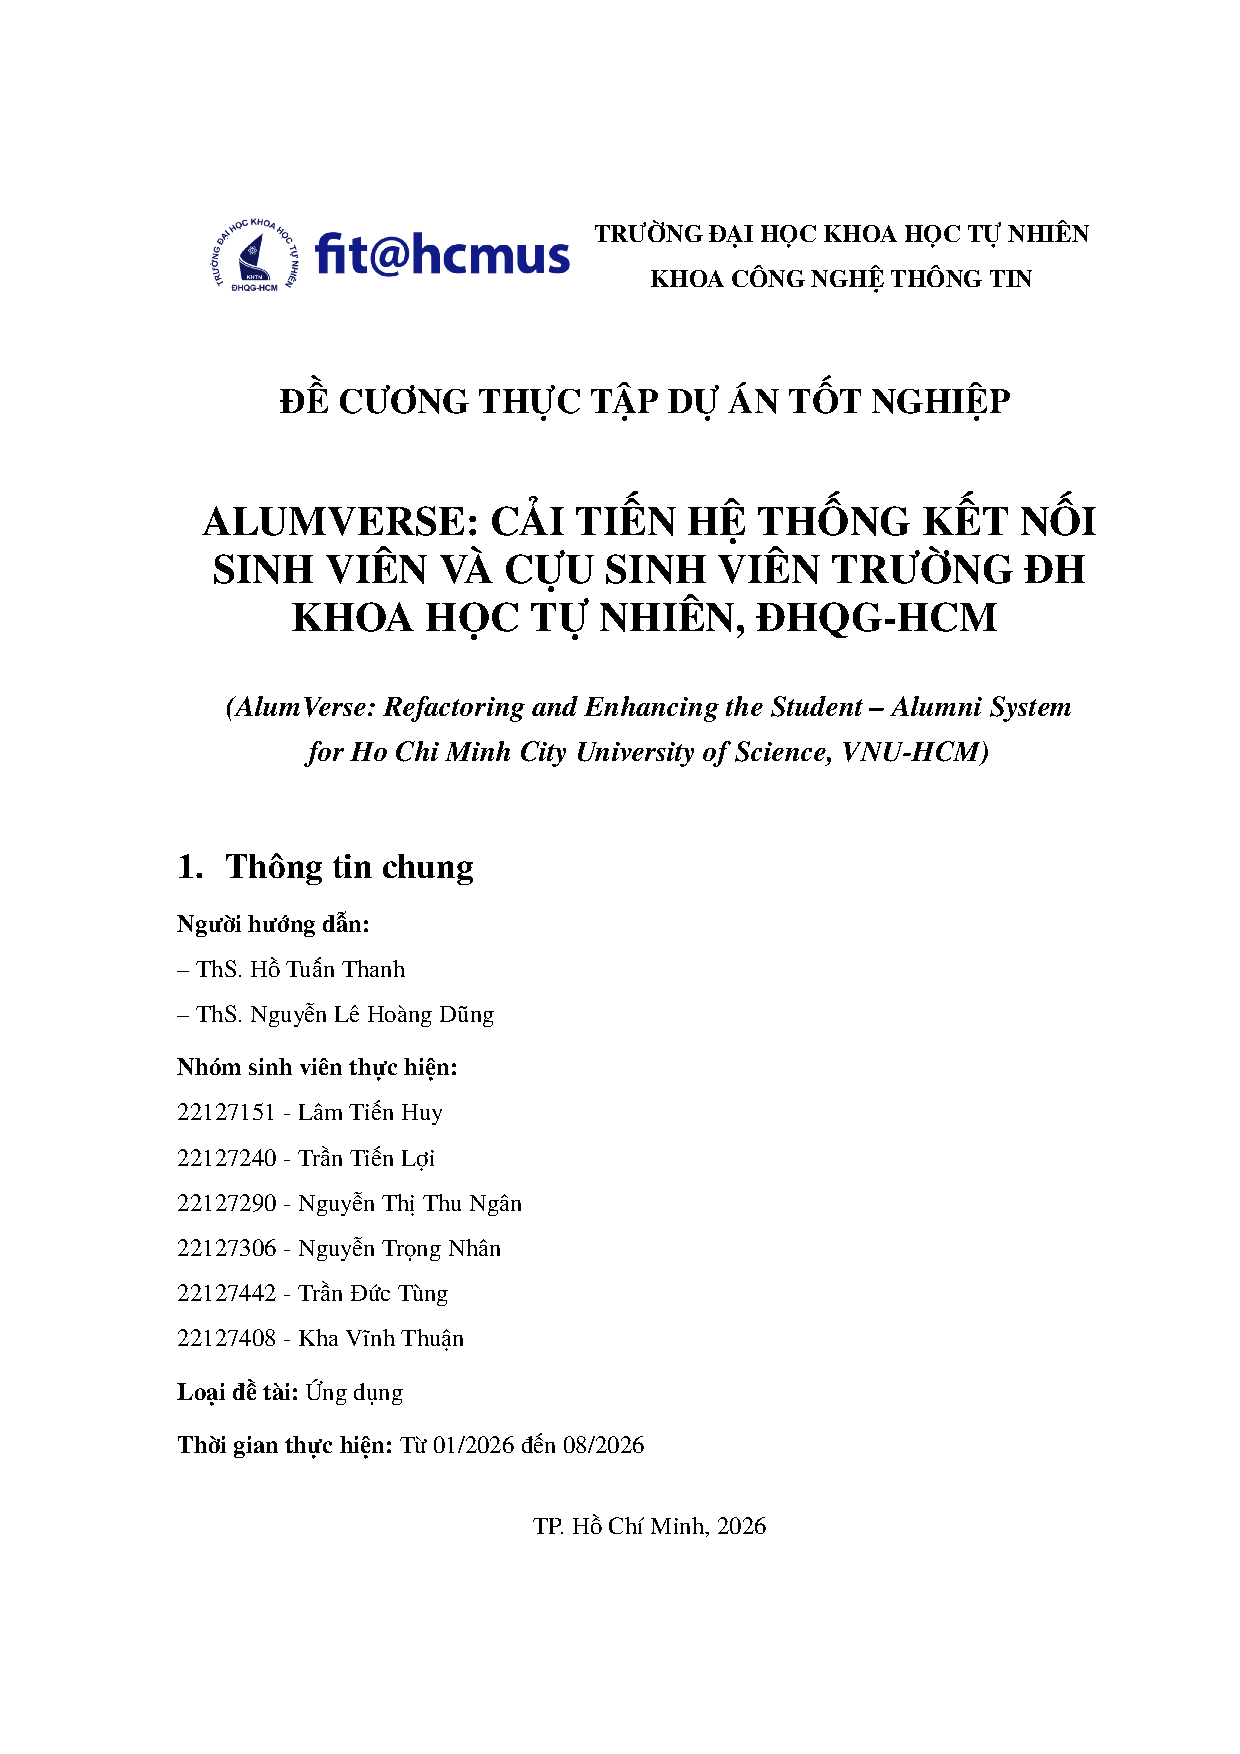
\includepdf[pages=-,pagecommand={\thispagestyle{empty}}]{AlumVerse_DeCuong_final.pdf}
\setcounter{page}{\value{dcpage}}

% ---------- MỤC LỤC ----------
\newpage
\renewcommand{\cfttoctitlefont}{\fontsize{14}{21}\selectfont\bfseries}
\renewcommand{\cftaftertoctitle}{\hfill}
\renewcommand{\cftloftitlefont}{\fontsize{14}{21}\selectfont\bfseries}
\renewcommand{\cftafterloftitle}{\hfill}
\renewcommand{\cftlottitlefont}{\fontsize{14}{21}\selectfont\bfseries}
\renewcommand{\cftafterlottitle}{\hfill}
\tableofcontents

\newpage
\listoffigures
\addcontentsline{toc}{chapter}{DANH MỤC HÌNH VẼ}

\newpage
\listoftables
\addcontentsline{toc}{chapter}{DANH MỤC BẢNG BIỂU}

% ---------- DANH MỤC VIẾT TẮT ----------
\newpage
\chapter*{DANH MỤC VIẾT TẮT VÀ THUẬT NGỮ}
\addcontentsline{toc}{chapter}{DANH MỤC VIẾT TẮT VÀ THUẬT NGỮ}

\renewcommand{\arraystretch}{1.3}
\begin{longtable}{|>{\raggedright\arraybackslash}p{3.2cm}|>{\raggedright\arraybackslash}p{11.3cm}|}
\hline
\textbf{Từ viết tắt / Thuật ngữ} & \textbf{Diễn giải} \\ \hline
\endfirsthead
\hline
\textbf{Từ viết tắt / Thuật ngữ} & \textbf{Diễn giải} \\ \hline
\endhead
API & Giao diện lập trình ứng dụng, tập hợp các điểm cuối cho phép các thành phần phần mềm trao đổi dữ liệu với nhau. \\ \hline
CI/CD & Quy trình tích hợp liên tục và triển khai liên tục, tự động hóa việc kiểm tra và đưa mã nguồn lên môi trường vận hành. \\ \hline
ERD & Sơ đồ thực thể và mối quan hệ, mô tả cấu trúc dữ liệu của hệ thống. \\ \hline
JWT & Chuẩn token dùng để truyền thông tin xác thực giữa client và máy chủ dưới dạng đã ký số. \\ \hline
Layered Architecture & Kiến trúc phân lớp, tổ chức mã nguồn thành các tầng có trách nhiệm tách biệt. \\ \hline
Modular Monolith & Kiến trúc trong đó hệ thống được triển khai như một ứng dụng duy nhất nhưng bên trong chia thành các module nghiệp vụ tách biệt. \\ \hline
Microservices & Kiến trúc chia ứng dụng thành nhiều dịch vụ nhỏ, triển khai độc lập, giao tiếp qua mạng. \\ \hline
Multi-tenant & Kiến trúc cho phép một hệ thống phục vụ đồng thời nhiều tổ chức với dữ liệu được cô lập. \\ \hline
OCR & Kỹ thuật nhận dạng ký tự quang học, trích xuất văn bản từ hình ảnh. \\ \hline
OTP & Mã dùng một lần, gửi qua email hoặc tin nhắn để xác thực người dùng. \\ \hline
R2DBC & Chuẩn kết nối cơ sở dữ liệu quan hệ theo cơ chế bất đồng bộ, không chặn luồng. \\ \hline
RAG & Kiến trúc kết hợp truy hồi tài liệu với mô hình ngôn ngữ để sinh câu trả lời có dẫn nguồn. \\ \hline
RBAC & Cơ chế phân quyền dựa trên vai trò của người dùng. \\ \hline
Reactive Programming & Mô hình lập trình xử lý dữ liệu theo luồng, bất đồng bộ và không chặn luồng. \\ \hline
SSE & Cơ chế cho phép máy chủ đẩy dữ liệu liên tục về trình duyệt trên một kết nối một chiều. \\ \hline
UAT & Thử nghiệm chấp nhận, do người dùng thực hiện nhằm xác nhận hệ thống đáp ứng nhu cầu thực tế. \\ \hline
WebSocket & Giao thức truyền dữ liệu hai chiều theo thời gian thực giữa client và máy chủ. \\ \hline
\end{longtable}
\renewcommand{\arraystretch}{1}

% ---------- TÓM TẮT ----------
\newpage
\chapter*{TÓM TẮT}
\addcontentsline{toc}{chapter}{TÓM TẮT}

Mạng lưới cựu sinh viên là nguồn lực chiến lược của các cơ sở giáo dục đại học, nhưng phần lớn nền tảng kết nối hiện nay, bao gồm cả phiên bản AlumVerse 2024 của Trường Đại học Khoa học Tự nhiên, được xây dựng theo mô hình mạng xã hội thuần túy nên tỉ lệ tương tác thực chất rất thấp và chưa khai thác được vai trò nghề nghiệp của cựu sinh viên. Bên cạnh đó, việc áp dụng kiến trúc Microservices quá sớm so với quy mô bài toán đã để lại khoản nợ kỹ thuật lớn, khiến chi phí triển khai và vận hành tăng cao.

Đề tài thực hiện cải tiến hệ thống AlumVerse theo hai hướng song song là tái thiết kế kiến trúc kỹ thuật và nâng cấp giá trị nghiệp vụ, đồng thời mở rộng hệ thống thành nền tảng đa đơn vị dùng chung cho nhiều khoa.

Về phương pháp, nhóm kế thừa kết quả phân tích, thiết kế và cấu trúc cơ sở dữ liệu của phiên bản 2024 nhưng xây dựng lại toàn bộ mã nguồn theo kiến trúc Modular Monolith kết hợp Layered trên nền Spring WebFlux và R2DBC, áp dụng mô hình Reactive Programming để xử lý bất đồng bộ. Hệ thống được phát triển đồng bộ trên web bằng React và trên di động bằng Flutter dùng chung một tầng API, với các luồng nghiệp vụ trọng tâm gồm chương trình cố vấn có cấu trúc kèm cơ chế chống trùng lịch, cổng việc làm và học liệu, gây quỹ có đối soát tự động qua webhook theo cơ chế idempotent, diễn đàn nghề nghiệp, và trợ lý ảo áp dụng kiến trúc RAG. Chất lượng được bảo đảm bằng kiểm thử đơn vị cho tầng nghiệp vụ, kiểm thử chức năng theo kịch bản người dùng và giám sát vận hành.

Kết quả, hệ thống hiện thực 86 tính năng thuộc 15 module trên 45 controller với 364 điểm cuối, trong đó 80 tính năng đã hoàn thiện, cùng 215 hàm kiểm thử đơn vị và 15 test case chức năng được tài liệu hóa; cơ chế cô lập dữ liệu đa đơn vị được kiểm chứng qua các kịch bản nhiều tổ chức.

Đề tài cho thấy việc lựa chọn kiến trúc phù hợp với quy mô thực tế, thay vì chạy theo kiến trúc phức tạp, mang lại hiệu quả rõ rệt về chi phí vận hành và khả năng bảo trì. Sản phẩm có thể triển khai cho các khoa thuộc Trường Đại học Khoa học Tự nhiên và cung cấp một khung tính năng có khả năng tái sử dụng cho các đơn vị đào tạo khác.

% ═══════════════════════════════════════════════════════════
%  PHẦN NỘI DUNG - ĐÁNH SỐ Ả-RẬP TỪ CHƯƠNG 1
% ═══════════════════════════════════════════════════════════
\newpage
\pagenumbering{arabic}
\setcounter{page}{1}

% ─────────────────────── CHƯƠNG 1 ───────────────────────
\chapter{MỞ ĐẦU}

\section{Đặt vấn đề}

Theo các nghiên cứu về vai trò của cựu sinh viên tại trường đại học \cite{obeng,unisel}, cựu sinh viên là nguồn tài nguyên quan trọng, có thể đóng góp trở lại cho nhà trường ở nhiều vai trò khác nhau như làm hình mẫu truyền cảm hứng cho sinh viên, cố vấn nghề nghiệp, chia sẻ chuyên môn, giới thiệu việc làm, đóng góp tài chính và góp phần xây dựng uy tín của nhà trường. Vì vậy, một hệ thống kết nối cựu sinh viên hiệu quả không chỉ giúp mọi người giữ liên lạc, mà còn giúp nhà trường khai thác được những giá trị mà các thế hệ đi trước có thể mang lại.

Tuy nhiên, phần lớn các nền tảng kết nối cựu sinh viên hiện nay được xây dựng giống như một mạng xã hội thu nhỏ, nơi người dùng chủ yếu vào xem và theo dõi thông tin nhưng rất ít khi tương tác thật sự. Thực tế quan sát tại nhiều nhóm và trang cộng đồng cựu sinh viên cho thấy số lượt tương tác trên mỗi bài đăng thường rất thấp so với quy mô thành viên. Những số liệu này được trình bày và phân tích chi tiết ở Chương 2, và đều cho thấy một điểm chung: mô hình đòi hỏi người dùng phải tương tác thường xuyên như mạng xã hội không phù hợp với cựu sinh viên, vốn là nhóm người dùng ít khi truy cập và hiếm khi tương tác công khai.

Hệ thống AlumVerse phiên bản 2024 \cite{alumverse}, sản phẩm của nhóm sinh viên khóa 2020 tại Trường Đại học Khoa học Tự nhiên, cũng được xây dựng theo hướng này. Hệ thống tập trung vào các chức năng mang tính nội dung và giao tiếp xã hội như tin tức, sự kiện, nhóm cộng đồng, nhắn tin và diễn đàn hỏi đáp, nhưng chưa có những tính năng tạo ra giá trị nghề nghiệp rõ ràng cho người dùng. Bên cạnh đó, hệ thống 2024 được xây dựng theo kiến trúc Microservices, vốn là một cách tổ chức phức tạp và tốn kém khi vận hành, không thực sự phù hợp với quy mô của một nền tảng cộng đồng phi lợi nhuận trong trường đại học.

Để khắc phục những hạn chế trên, một hệ thống kết nối cựu sinh viên hiệu quả cần đáp ứng tốt nhu cầu của ba nhóm người dùng chính. Về phía nhà trường, các đơn vị quản lý ở cấp trường và cấp khoa cần quản lý dữ liệu sinh viên và cựu sinh viên một cách có hệ thống, đồng thời thống kê tỉ lệ việc làm của sinh viên tốt nghiệp để phục vụ công tác báo cáo theo quy định của Bộ Giáo dục và Đào tạo \cite{moet}. Về phía cựu sinh viên, họ có nhu cầu kết nối lại với bạn bè cũ, tham gia các sự kiện gắn kết, tìm kiếm cơ hội việc làm và học tập suốt đời. Về phía sinh viên, nhu cầu nổi bật là giải đáp các vấn đề về việc học, định hướng lộ trình nghề nghiệp và được cố vấn từ người đi trước. Nhiều nghiên cứu đã khẳng định giá trị tích cực của hoạt động cố vấn đối với quá trình định hướng và chuyển tiếp nghề nghiệp của sinh viên \cite{nabi}. Đồng thời, nhu cầu tìm kiếm người cố vấn ngày càng tăng và mô hình kết nối giữa người cố vấn và người được cố vấn đã trở nên phổ biến, trải rộng nhiều ngành nghề, trên cả các nền tảng quốc tế \cite{adplist} lẫn các cộng đồng nghề nghiệp tại Việt Nam \cite{mentori}. Những nhu cầu này được phân tích chi tiết ở Chương 2.

Đề tài này kế thừa hệ thống AlumVerse 2024 và tập trung cải tiến theo hai hướng song song. Một mặt, nhóm tái thiết kế phần kỹ thuật để hệ thống đơn giản hơn, ổn định hơn và ít tốn chi phí hơn khi vận hành. Mặt khác, nhóm thay đổi trọng tâm của sản phẩm: thay vì cố gắng tạo ra một mạng xã hội có nhiều lượt tương tác, hệ thống tập trung vào những giá trị thiết thực mà cựu sinh viên và sinh viên thật sự cần, những giá trị vẫn có ích ngay cả khi người dùng chỉ thỉnh thoảng truy cập. Nói cách khác, AlumVerse 2026 vừa khắc phục hạn chế của phiên bản 2024, vừa đáp ứng nhu cầu khác nhau của các nhóm người dùng nêu trên. Đây là định hướng xuyên suốt của đề tài.

\section{Mục tiêu đề tài}

Đề tài tập trung cải tiến hệ thống AlumVerse theo hai hướng chính, cũng là hai nhóm đóng góp của nhóm thực hiện về mặt kỹ thuật và nghiệp vụ.

Hướng thứ nhất là tái thiết kế kỹ thuật. Nhóm chuyển hệ thống từ kiến trúc Microservices với chín dịch vụ Spring Boot, Eureka, API Gateway và MySQL sang kiến trúc Modular Monolith kết hợp Layered trên nền Spring WebFlux, R2DBC và PostgreSQL. Việc chuyển đổi này không chỉ khắc phục các tính năng còn lỗi hoặc chậm mà còn tối ưu hóa hiệu năng, khả năng bảo trì và đặc biệt là tài nguyên phần cứng, từ đó hạ đáng kể chi phí vận hành cho một nền tảng phi lợi nhuận của trường đại học.

Hướng thứ hai là nâng cao giá trị nghiệp vụ và trải nghiệm người dùng. Nhóm hiện thực hóa các tính năng giúp phát huy vai trò của cựu sinh viên, đồng thời xây dựng khung tính năng có khả năng tái sử dụng cao thông qua mô hình Multi-tenant. Các nhóm tính năng trọng tâm bao gồm chương trình cố vấn có cấu trúc, cơ hội việc làm và học tập suốt đời, gây quỹ minh bạch, diễn đàn nghề nghiệp, khảo sát phục vụ thống kê việc làm và trợ lý ảo.

Cụ thể, đề tài hướng đến năm mục tiêu sau:

\begin{enumerate}[label=(\arabic*),leftmargin=1.4cm,itemsep=2pt]
\item Khảo sát nhu cầu người dùng và phân tích hiện trạng hệ thống AlumVerse 2024, từ đó xác định khoảng trống và các vấn đề cần giải quyết.
\item Nghiên cứu, đánh giá và lựa chọn kiến trúc phần mềm phù hợp nhằm giải quyết các rào cản về hiệu năng của hệ thống cũ, đồng thời đáp ứng yêu cầu triển khai đa đơn vị và tối ưu chi phí.
\item Phân tích, thiết kế và triển khai các tính năng theo từng nhóm nghiệp vụ, bảo đảm có căn cứ rõ ràng để đánh giá mức độ hoàn thành.
\item Phát triển ứng dụng web trên nền React và ứng dụng di động trên nền Flutter, dùng chung một hệ thống API.
\item Kiểm chứng hiệu quả của kiến trúc mới thông qua đánh giá hiệu năng và đối chiếu với các hạn chế kỹ thuật đã được ghi nhận ở hệ thống 2024.
\end{enumerate}

\section{Đối tượng và phạm vi nghiên cứu}

\subsection{Đối tượng nghiên cứu}

Đối tượng nghiên cứu cốt lõi của đề tài là các quy trình nghiệp vụ nhằm kết nối giá trị giữa sinh viên và cựu sinh viên, cùng với kiến trúc phần mềm đáp ứng được sự linh hoạt của các quy trình đó.

Do kế thừa và phát triển từ một hệ thống đã có sẵn, đề tài tiếp tục phục vụ các nhóm người dùng đã được định hình từ phiên bản 2024, bao gồm sinh viên và cựu sinh viên của Trường Đại học Khoa học Tự nhiên; đội ngũ cán bộ và quản trị viên ở cấp khoa và cấp trường, phụ trách quản lý nội dung, tổ chức sự kiện, xác minh danh tính và điều phối các chương trình; và khách vãng lai chưa đăng nhập với quyền truy cập giới hạn nhằm mở rộng khả năng tiếp cận thông tin công khai.

\subsection{Phạm vi nghiên cứu}

Đề tài bao trùm toàn bộ chu trình phát triển sản phẩm với các giới hạn kỹ thuật cụ thể sau.

Về hệ thống phần mềm, nhóm xây dựng backend, ứng dụng web chạy tốt trên nhiều kích thước màn hình bằng React, cùng ứng dụng di động độc lập bằng Flutter; tất cả các nền tảng dùng chung một hệ thống API.

Về hạ tầng và dữ liệu, hệ thống sử dụng PostgreSQL làm hệ quản trị cơ sở dữ liệu, đóng gói và triển khai thông qua Docker Compose và Nginx.

Về kiến trúc đa đơn vị, hệ thống áp dụng mô hình Multi-tenant ở mức chia sẻ cơ sở dữ liệu và chia sẻ lược đồ, phân tách dữ liệu giữa các khoa thông qua cột định danh \texttt{organization\_id}.

\subsection{Giới hạn và các nội dung chủ động loại trừ}

Khác với việc cắt giảm chức năng do thiếu hụt nguồn lực, đề tài chủ động loại bỏ và giới hạn một số cấu trúc kỹ thuật từng có ở phiên bản 2024 nhằm bám sát nguyên tắc thiết kế tinh gọn, hạ chi phí vận hành và phù hợp với thực tiễn nghiệp vụ.

Thứ nhất, hệ thống không phân tách cơ sở dữ liệu vật lý cho từng khoa. Mô hình Multi-tenant được triển khai ở mức chia sẻ cơ sở dữ liệu. Vì các khoa cùng trực thuộc sự quản lý tập trung của nhà trường và tái sử dụng chung một bộ khung nghiệp vụ, việc gộp các dịch vụ về một ứng dụng duy nhất và dùng chung cơ sở dữ liệu giúp loại bỏ sự cồng kềnh của hạ tầng, tối ưu chi phí mà vẫn bảo đảm tính cô lập dữ liệu ở mức logic.

Thứ hai, hệ thống loại bỏ cơ chế phân quyền động. Phiên bản 2024 cho phép tạo và sửa quyền truy cập linh động theo từng vai trò qua giao diện. Thực tế vận hành cho thấy tệp người dùng của một nền tảng cựu sinh viên là cố định, gồm sinh viên, cựu sinh viên, quản trị cấp khoa và quản trị toàn hệ thống. Việc tinh gọn bằng tập quyền cố định giúp tăng tốc độ truy vấn, loại bỏ các thao tác kết nối nhiều bảng không cần thiết và tránh tình trạng thiết kế phức tạp quá mức mà không tạo ra giá trị khác biệt cho người dùng cuối.

\section{Cấu trúc báo cáo}

Phần còn lại của báo cáo được tổ chức thành năm chương. Chương 2 trình bày cơ sở lý thuyết, các công nghệ nền tảng và khảo sát hiện trạng, bao gồm phân tích hệ thống 2024, kết quả khảo sát người dùng và đề xuất hướng giải quyết. Chương 3 trình bày quá trình phân tích yêu cầu và thiết kế hệ thống, gồm tác nhân, yêu cầu chức năng, kiến trúc, cơ sở dữ liệu và giao diện đa nền tảng. Chương 4 mô tả môi trường triển khai, quy trình phát triển của nhóm và cách xây dựng các luồng nghiệp vụ quan trọng. Chương 5 trình bày quá trình thử nghiệm và đánh giá, gồm kiểm thử chức năng, đánh giá mức độ hoàn thành, đánh giá hiệu năng và đối chiếu với hệ thống 2024. Chương 6 tổng kết các kết quả đã đạt được, nhìn nhận những hạn chế còn tồn tại và đề xuất định hướng phát triển trong tương lai.

% ─────────────────────── CHƯƠNG 2 ───────────────────────
\chapter{CƠ SỞ LÝ THUYẾT VÀ HIỆN TRẠNG}

Chương này trình bày cơ sở lý thuyết và công nghệ nền tảng làm căn cứ cho các quyết định kỹ thuật của đề tài, phân tích vai trò của cựu sinh viên và nhu cầu của các nhóm người dùng, khảo sát các hệ thống liên quan, và phân tích hiện trạng hệ thống AlumVerse phiên bản 2024. Trên cơ sở đó, chương xác định các khoảng trống cần giải quyết và đề xuất định hướng giải pháp cho phiên bản 2026.

\section{Cơ sở lý thuyết và công nghệ nền tảng}

\subsection{Tái thiết kế và xử lý nợ kỹ thuật}

Nợ kỹ thuật là khái niệm chỉ những chi phí phát sinh trong tương lai do việc ưu tiên các giải pháp phát triển nhanh thay vì một thiết kế bền vững lâu dài \cite{cunningham,fowlerref}. Tại hệ thống AlumVerse phiên bản 2024, nợ kỹ thuật xuất phát chủ yếu từ việc áp dụng kiến trúc Microservices quá sớm so với quy mô bài toán, dẫn đến sự phụ thuộc phức tạp giữa các dịch vụ và làm tăng đáng kể chi phí triển khai lẫn vận hành.

Qua đánh giá hiện trạng, nhóm nhận định việc chỉnh sửa trực tiếp trên nền tảng cũ sẽ không giải quyết được triệt để các nút thắt về hiệu năng, bởi nguyên nhân nằm ở lựa chọn kiến trúc chứ không nằm ở từng đoạn mã cụ thể. Đồng thời, do không trực tiếp tiếp nhận mã nguồn của khóa trước, nhóm quyết định phát triển mới hoàn toàn. Thay vì tái sử dụng mã nguồn, nhóm kế thừa các tài sản phân tích cốt lõi từ tài liệu của khóa trước \cite{alumverse}, bao gồm đặc tả tính năng, kiến trúc nghiệp vụ và cấu trúc cơ sở dữ liệu. Đây là phần phản ánh đúng bài toán kết nối đặc thù tại Trường Đại học Khoa học Tự nhiên nên vẫn giữ nguyên giá trị.

Trên nền tảng kế thừa đó, toàn bộ mã nguồn được xây dựng lại theo kiến trúc Modular Monolith. Cơ sở dữ liệu được tái thiết kế trên PostgreSQL, kết hợp giữa việc chuẩn hóa lược đồ cũ và mở rộng cho các nhóm tính năng mới. Giao tiếp giữa các tầng ứng dụng được quy chuẩn hóa và chuyển hoàn toàn sang mô hình xử lý bất đồng bộ.

Như vậy, từ khóa refactoring trong tên đề tài cần được hiểu là tái thiết kế ở cấp độ kiến trúc, được hiện thực hóa bằng việc xây dựng lại hệ thống dựa trên khung phân tích đã có, chứ không phải tinh chỉnh mã nguồn theo cách hiểu truyền thống của thuật ngữ này.

\subsection{Kiến trúc Modular Monolith và Layered}

Microservices \cite{microservices} chia một ứng dụng thành nhiều dịch vụ nhỏ, độc lập, giao tiếp qua mạng. Cách tổ chức này phù hợp với hệ thống quy mô rất lớn và nhiều đội phát triển song song, nhưng làm tăng đáng kể độ phức tạp khi triển khai, giám sát và gỡ lỗi ở các dự án quy mô vừa.

Modular Monolith giữ hệ thống là một ứng dụng duy nhất khi triển khai, bên trong chia thành các module nghiệp vụ tách biệt với ranh giới trách nhiệm rõ ràng. Kết hợp với kiến trúc Layered \cite{poeaa}, mỗi module được tổ chức theo các lớp controller, service, dao, entity và dto. Cách tổ chức này vẫn giữ được sự tách bạch trách nhiệm của Microservices nhưng loại bỏ chi phí vận hành của một hệ phân tán, đồng thời bảo toàn khả năng tách thành dịch vụ độc lập về sau nếu quy mô thực sự đòi hỏi.

Đề cương ban đầu dự kiến áp dụng Clean Architecture \cite{clean} với các tầng use-case, port và adapter. Thực tế triển khai cho thấy chi phí ánh xạ dữ liệu giữa các tầng và chi phí viết kiểm thử tăng đáng kể so với lợi ích thu được ở quy mô đề tài. Nhóm điều chỉnh sang Modular Monolith kết hợp Layered nhằm phù hợp với nguồn lực và tiến độ mà vẫn bảo đảm khả năng bảo trì, mở rộng. Quyết định điều chỉnh này được ghi nhận trong Báo cáo tiến độ.

\subsection{Reactive Programming}

Mô hình Reactive Programming được đặc trưng bởi bốn tính chất cốt lõi là phản hồi nhanh, có khả năng phục hồi, co giãn linh hoạt và hướng thông điệp \cite{reactive}. Spring WebFlux hiện thực hóa mô hình này thông qua thư viện Project Reactor với hai kiểu dữ liệu Mono và Flux, cho phép xử lý yêu cầu theo cơ chế bất đồng bộ và không chặn luồng. Ở tầng truy cập dữ liệu, R2DBC tương tác với cơ sở dữ liệu quan hệ theo cùng cơ chế bất đồng bộ, thay thế cho phương thức kết nối đồng bộ truyền thống.

Nhờ cơ chế không chặn luồng, hệ thống duy trì được đồng thời số lượng lớn kết nối mà chỉ tiêu tốn một lượng luồng xử lý tối thiểu. Đặc điểm này đặc biệt quan trọng với các tính năng đòi hỏi luồng dữ liệu duy trì liên tục như nhắn tin thời gian thực và trợ lý ảo trả lời theo dòng. Sự kết hợp giữa Spring WebFlux và R2DBC nhằm giải quyết nút thắt về tài nguyên khi lưu lượng truy cập tăng đột biến, vốn là hạn chế của mô hình Servlet đồng bộ ở phiên bản 2024.

Đổi lại, kiến trúc này đi kèm rào cản học tập cao hơn và chi phí gỡ lỗi lớn hơn do vết gọi hàm không còn tuyến tính. Nhóm chấp nhận sự đánh đổi này để bám sát định hướng tối ưu hóa hiệu năng và tài nguyên phần cứng đã đề ra.

\subsection{Kiến trúc Multi-tenant}

Kiến trúc đa đơn vị phục vụ nhiều tổ chức trên cùng một nền tảng có ba phương pháp quản lý dữ liệu: mỗi đơn vị một cơ sở dữ liệu vật lý riêng; dùng chung cơ sở dữ liệu nhưng tách biệt lược đồ cho từng đơn vị; hoặc dùng chung cả cơ sở dữ liệu lẫn lược đồ và phân biệt dữ liệu thông qua một cột định danh \cite{multitenant}. Ba phương pháp phản ánh sự đánh đổi trực tiếp giữa mức độ cô lập dữ liệu và chi phí vận hành.

Hệ thống AlumVerse lựa chọn phương pháp thứ ba, phân tách dữ liệu của từng đơn vị thông qua cột định danh \texttt{organization\_id}. Ở tầng giao diện, mỗi tổ chức được nhận diện qua đường dẫn riêng, ví dụ \texttt{alumverse.hcmus.edu.vn/fit}. Ở tầng máy chủ, định danh tổ chức được nhúng trực tiếp vào token xác thực và đóng vai trò điều kiện lọc bắt buộc ở mọi truy vấn, thay vì tin tưởng giá trị do phía client gửi lên.

Lựa chọn này phù hợp với quy mô hiện tại của dự án. Các khoa cùng trực thuộc sự quản lý tập trung của nhà trường và tái sử dụng chung một bộ khung nghiệp vụ, nên mức cô lập logic đã đáp ứng yêu cầu, trong khi việc tách cơ sở dữ liệu vật lý cho từng đơn vị sẽ làm chi phí vận hành tăng lên mà không tạo thêm giá trị tương xứng.

\subsection{Retrieval-Augmented Generation}

Các mô hình ngôn ngữ lớn sinh câu trả lời dựa trên tri thức đã học trong quá trình huấn luyện. Cách vận hành này bộc lộ ba hạn chế khi áp dụng vào hệ thống thông tin của một tổ chức cụ thể: mô hình không biết các tài liệu nội bộ chưa từng xuất hiện trong dữ liệu huấn luyện; tri thức của mô hình bị đóng băng tại thời điểm huấn luyện; và mô hình có xu hướng sinh ra câu trả lời nghe hợp lý nhưng sai sự thật khi không đủ thông tin.

Retrieval-Augmented Generation là kiến trúc bổ sung một bước truy hồi thông tin trước bước sinh câu trả lời nhằm khắc phục các hạn chế trên \cite{rag}. Quy trình gồm hai giai đoạn. Giai đoạn nạp dữ liệu tách tài liệu thành các đoạn văn bản ngắn, chuyển mỗi đoạn thành một vector biểu diễn ngữ nghĩa thông qua mô hình embedding, rồi lưu vào cơ sở dữ liệu vector. Giai đoạn trả lời chuyển câu hỏi của người dùng thành vector theo cùng mô hình embedding, tìm những đoạn có độ tương đồng ngữ nghĩa cao nhất, sắp xếp lại kết quả theo mức độ liên quan nếu cần, rồi đưa các đoạn này vào ngữ cảnh của lời nhắc để mô hình ngôn ngữ sinh câu trả lời.

Kiến trúc này mang lại ba lợi ích phù hợp với bài toán của đề tài. Thứ nhất, tri thức của trợ lý ảo được cập nhật bằng cách bổ sung tài liệu vào kho dữ liệu, không cần huấn luyện lại mô hình. Thứ hai, câu trả lời bị ràng buộc trong phạm vi tài liệu đã truy hồi nên giảm đáng kể hiện tượng bịa đặt thông tin. Thứ ba, hệ thống có thể dẫn nguồn tài liệu cho từng câu trả lời, giúp người dùng kiểm chứng.

Cần phân biệt hai cách ứng dụng mô hình ngôn ngữ trong AlumVerse. Trợ lý ảo FitBot áp dụng kiến trúc RAG vì phải trả lời dựa trên kho tài liệu riêng của nhà trường và cần dẫn được nguồn. Ngược lại, các tác vụ như trích xuất kỹ năng từ mô tả chuyên môn, trích xuất thông tin từ hồ sơ năng lực, làm sạch kết quả nhận dạng ký tự quang học, kiểm duyệt nội dung và tự động gắn thẻ bài viết không cần truy hồi tài liệu, nên được hiện thực bằng lời gọi mô hình ngôn ngữ trực tiếp với đầu ra có cấu trúc. Chi tiết hiện thực của cả hai nhóm được trình bày ở Chương 4.

\section{Phân tích vai trò của cựu sinh viên và nhu cầu các nhóm người dùng}

\subsection{Vai trò của cựu sinh viên đối với nhà trường}

Các nghiên cứu về vai trò của cựu sinh viên chỉ ra rằng cựu sinh viên có thể đóng góp cho nhà trường ở nhiều vai trò khác nhau, bao gồm làm hình mẫu truyền cảm hứng, cố vấn nghề nghiệp, đóng góp chuyên môn, hỗ trợ phát triển nghề nghiệp cho thế hệ sau, tham gia tuyển dụng, đóng góp tài chính và góp phần xây dựng uy tín của nhà trường. Bảy vai trò này là cơ sở để xác định các nhóm tính năng hướng giá trị của AlumVerse, thay vì chỉ dừng lại ở các chức năng tương tác xã hội.

\subsection{Nhu cầu của nhóm quản trị}

Ở cấp trường và cấp khoa, các đơn vị quản lý cần một công cụ để quản lý hồ sơ sinh viên và cựu sinh viên một cách có hệ thống, xác minh danh tính và phân nhóm theo khoa, theo khóa, thay cho cách lưu trữ rời rạc trên mạng xã hội hoặc bảng tính.

Việc thống kê tỉ lệ sinh viên có việc làm sau khi tốt nghiệp là một nhu cầu có cơ sở pháp lý. Theo quy định của Bộ Giáo dục và Đào tạo, các cơ sở giáo dục đại học phải khảo sát, công khai và báo cáo tình hình việc làm của sinh viên sau một năm tốt nghiệp; báo cáo được nộp trước ngày 31 tháng 12 hằng năm và là một trong những căn cứ để xác định chỉ tiêu tuyển sinh. Một nền tảng kết nối cựu sinh viên có thể hỗ trợ trực tiếp nhu cầu này thông qua việc quản lý dữ liệu theo khóa, phát phiếu khảo sát và tổng hợp thông tin việc làm. Đây là căn cứ để AlumVerse xây dựng module khảo sát như một nhóm tính năng độc lập, chứ không chỉ là chức năng phụ trợ.

Nhà trường cũng cần một kênh chính thức để truyền thông tin tức, tổ chức sự kiện, vinh danh thành tích và tiếp nhận đóng góp, gây quỹ một cách minh bạch.

\subsection{Nhu cầu của nhóm cựu sinh viên}

Cựu sinh viên có nhu cầu kết nối lại với bạn bè cũ, ôn lại kỷ niệm và mở rộng quan hệ nghề nghiệp. Họ cũng mong muốn tham gia các sự kiện gắn kết định kỳ, đôi khi đi kèm mô hình hội viên có thu phí và quyền lợi tương ứng. Chương trình RMIT Active Hub của Trường Đại học RMIT Việt Nam là một ví dụ: cựu sinh viên đóng phí theo học kỳ để sử dụng cơ sở vật chất, dịch vụ và câu lạc bộ, qua đó duy trì kết nối với trường (Hình \ref{fig:rmit}) \cite{rmit}.

\begin{figure}[H]\centering
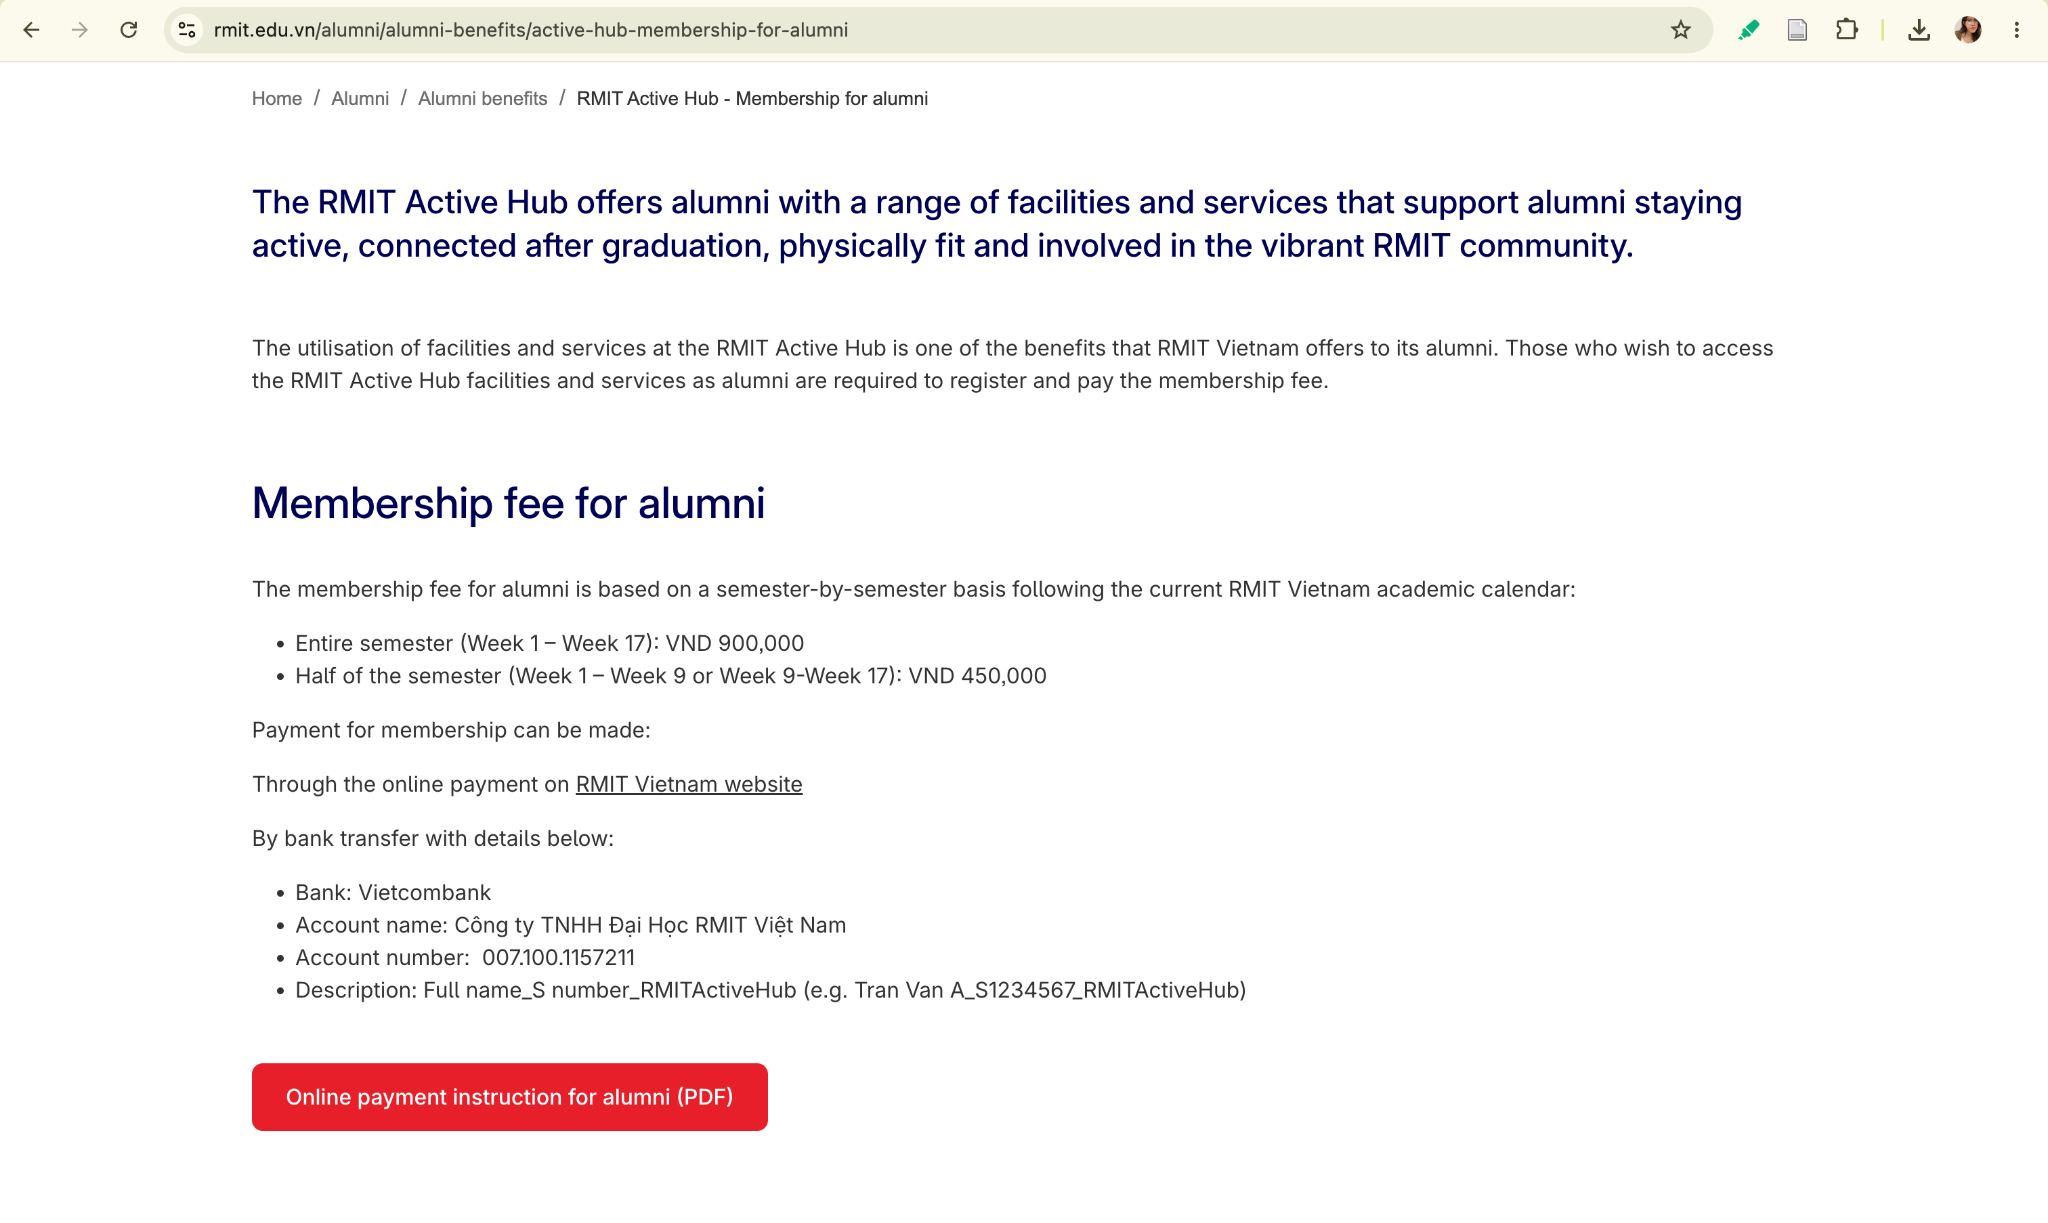
\includegraphics[width=0.90\textwidth,keepaspectratio]{hinh-2-1_rmit-active-hub}
\caption{Trang quyền lợi hội viên của chương trình RMIT Active Hub}
\label{fig:rmit}
\end{figure}

Mô hình hội viên trả phí gắn với cơ sở vật chất phù hợp với các trường có hạ tầng lớn và khó áp dụng cho phần lớn trường đại học công lập tại Việt Nam. Ở các trường công lập, hoạt động gắn kết cựu sinh viên chủ yếu xoay quanh các sự kiện gặp mặt. Tại Khoa Công nghệ Thông tin, Trường Đại học Khoa học Tự nhiên, các hoạt động này gồm ngày hội cựu sinh viên, giải thể thao truyền thống, câu lạc bộ cựu sinh viên, các buổi seminar chia sẻ kinh nghiệm và quỹ học bổng hỗ trợ sinh viên (Hình \ref{fig:fit}) \cite{fithcmus}. AlumVerse hướng theo mô hình này và phục vụ các nhu cầu đó qua module sự kiện, mạng lưới kết nối, cố vấn và gây quỹ, thay vì mô hình hội viên trả phí.

\begin{figure}[H]\centering
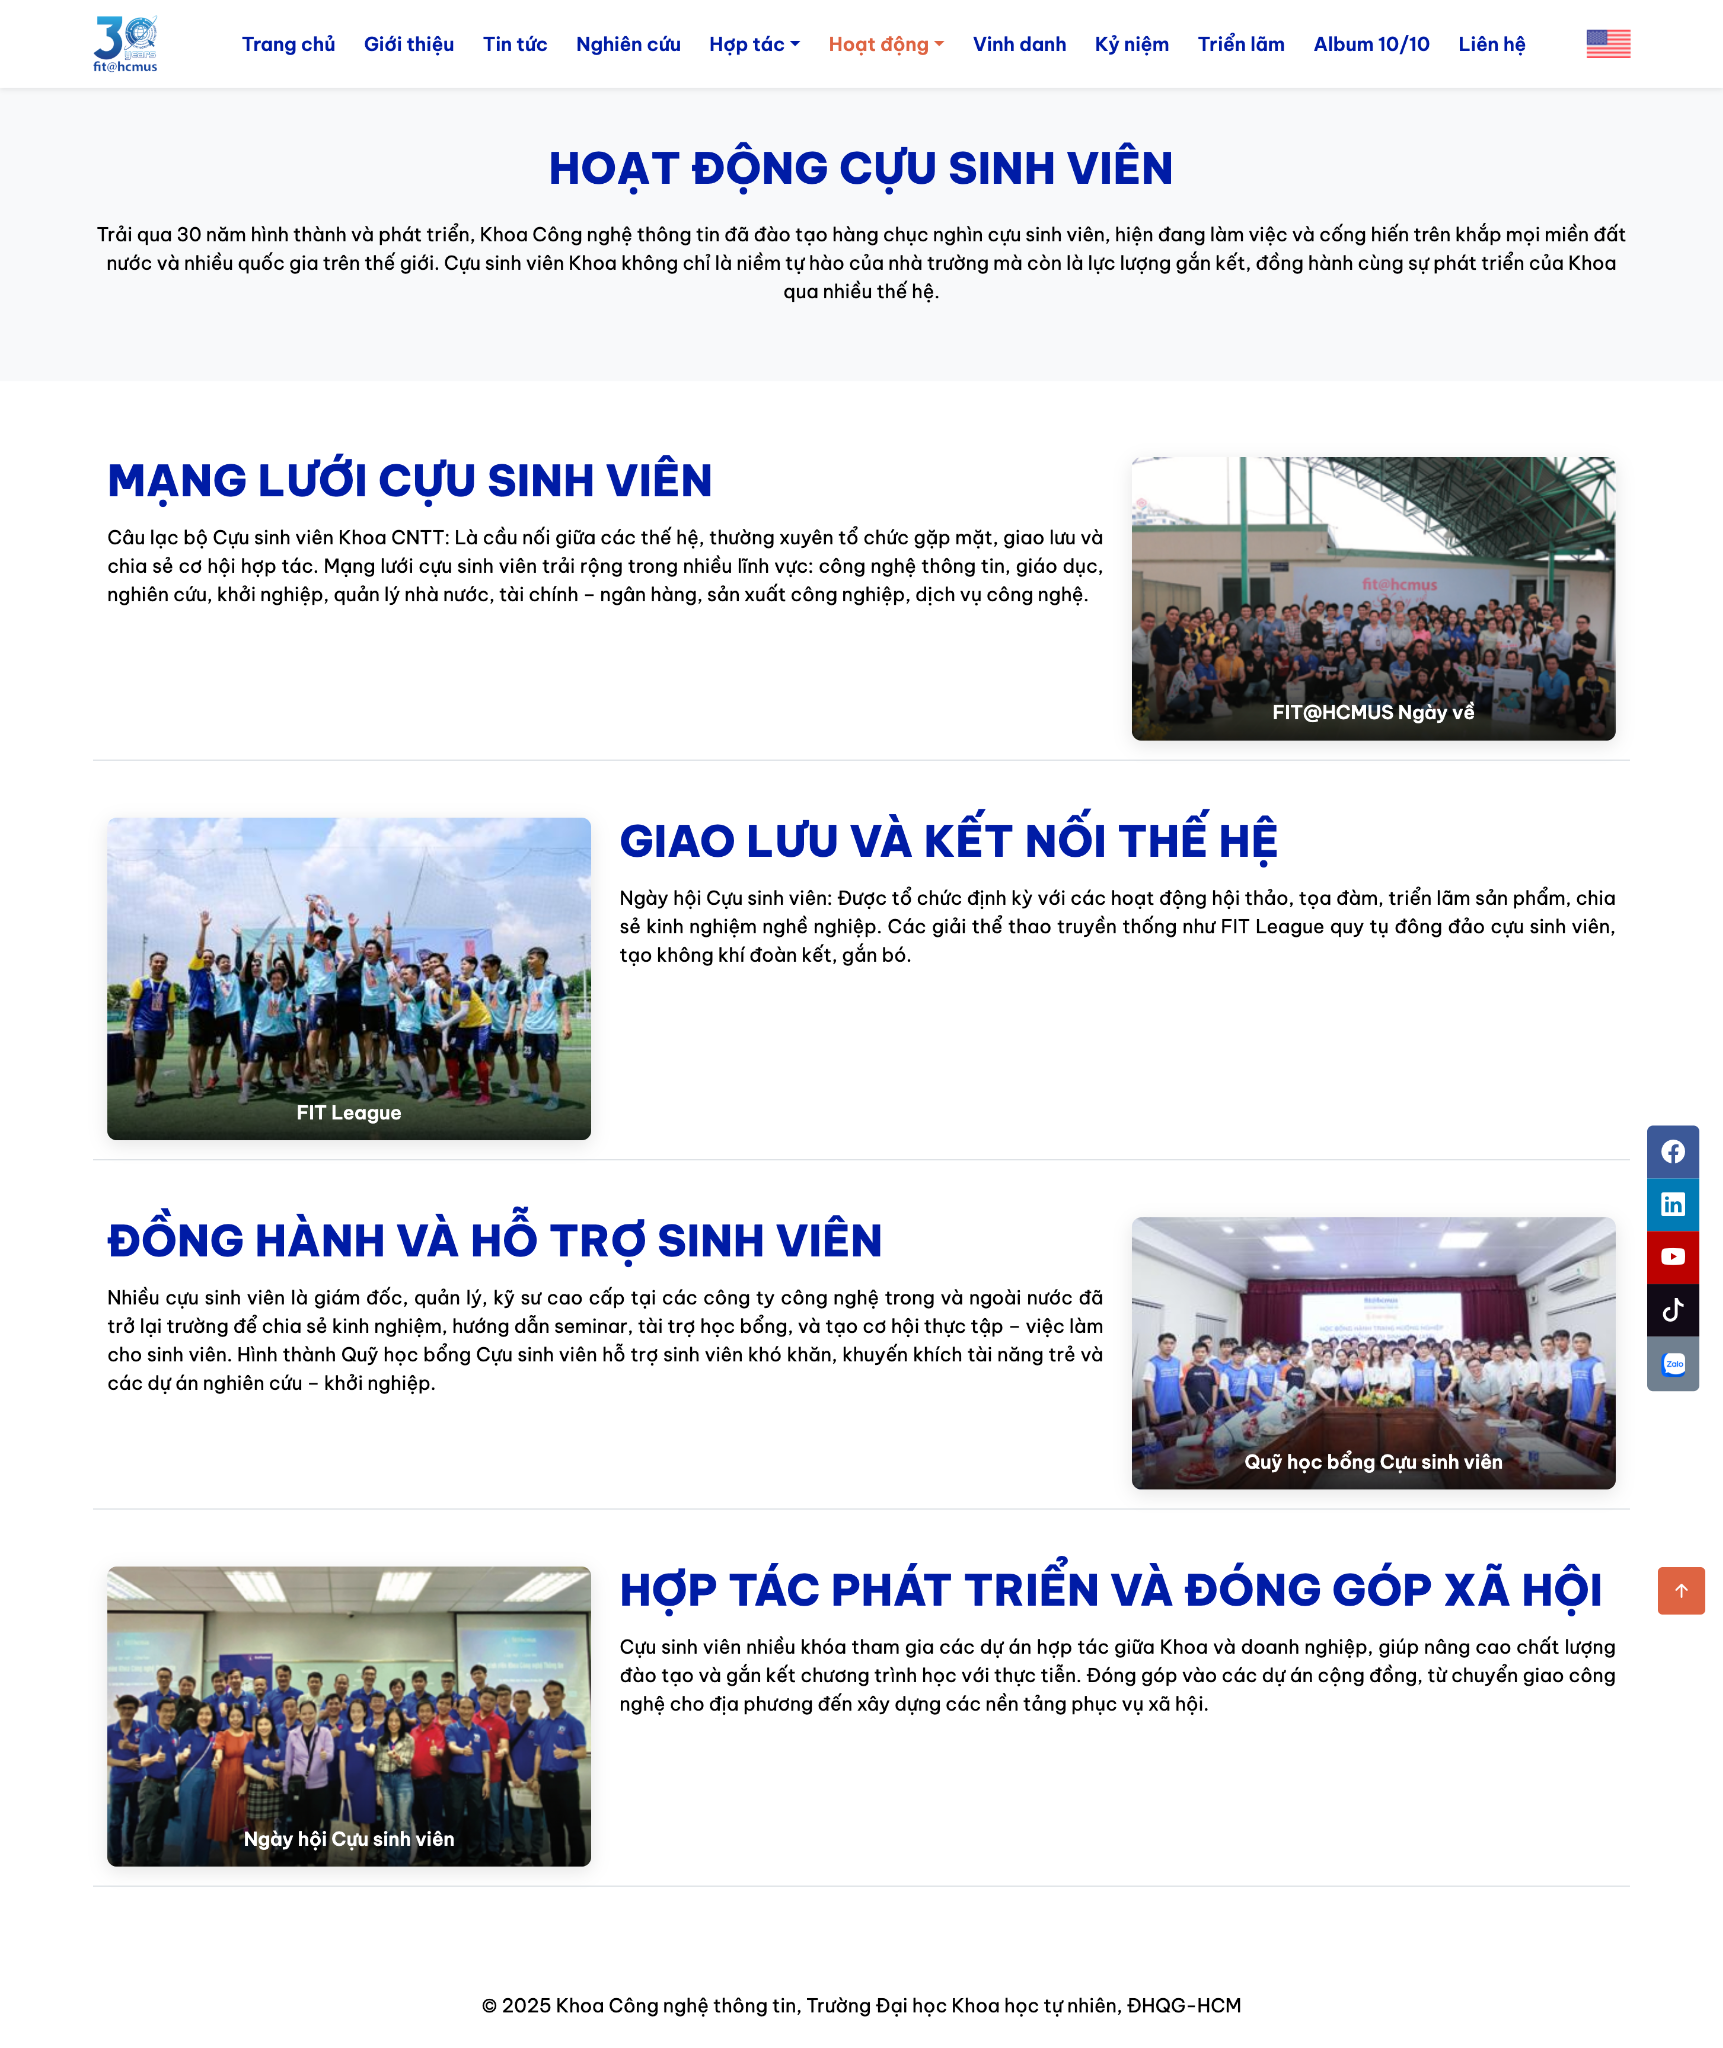
\includegraphics[width=0.90\textwidth,keepaspectratio]{hinh-2-2_fit-hcmus-alumni}
\caption{Trang hoạt động cựu sinh viên của Khoa Công nghệ Thông tin}
\label{fig:fit}
\end{figure}

Bên cạnh nhu cầu gắn kết, cựu sinh viên còn quan tâm đến cơ hội việc làm, giới thiệu việc làm và học tập suốt đời thông qua chia sẻ kỹ năng, khóa học và thông tin học sau đại học.

\subsection{Nhu cầu của nhóm sinh viên}

Sinh viên đang theo học có nhu cầu lớn trong việc được giải đáp học thuật, định hướng lộ trình nghề nghiệp và tìm kiếm sự dẫn dắt từ thế hệ đi trước. Một báo cáo tổng quan phân tích 73 nghiên cứu khoa học đã khẳng định hoạt động cố vấn có tác động tích cực đến quá trình lựa chọn nghề nghiệp và bước chuyển tiếp từ giảng đường sang thị trường lao động của sinh viên.

Trên thực tế, mô hình ghép cặp cố vấn đã chứng minh được hiệu quả và được ứng dụng rộng rãi. Ở quy mô toàn cầu, nền tảng ADPList thu hút hơn 40.000 chuyên gia đến từ trên 140 quốc gia (Hình \ref{fig:adplist}).

\begin{figure}[H]\centering
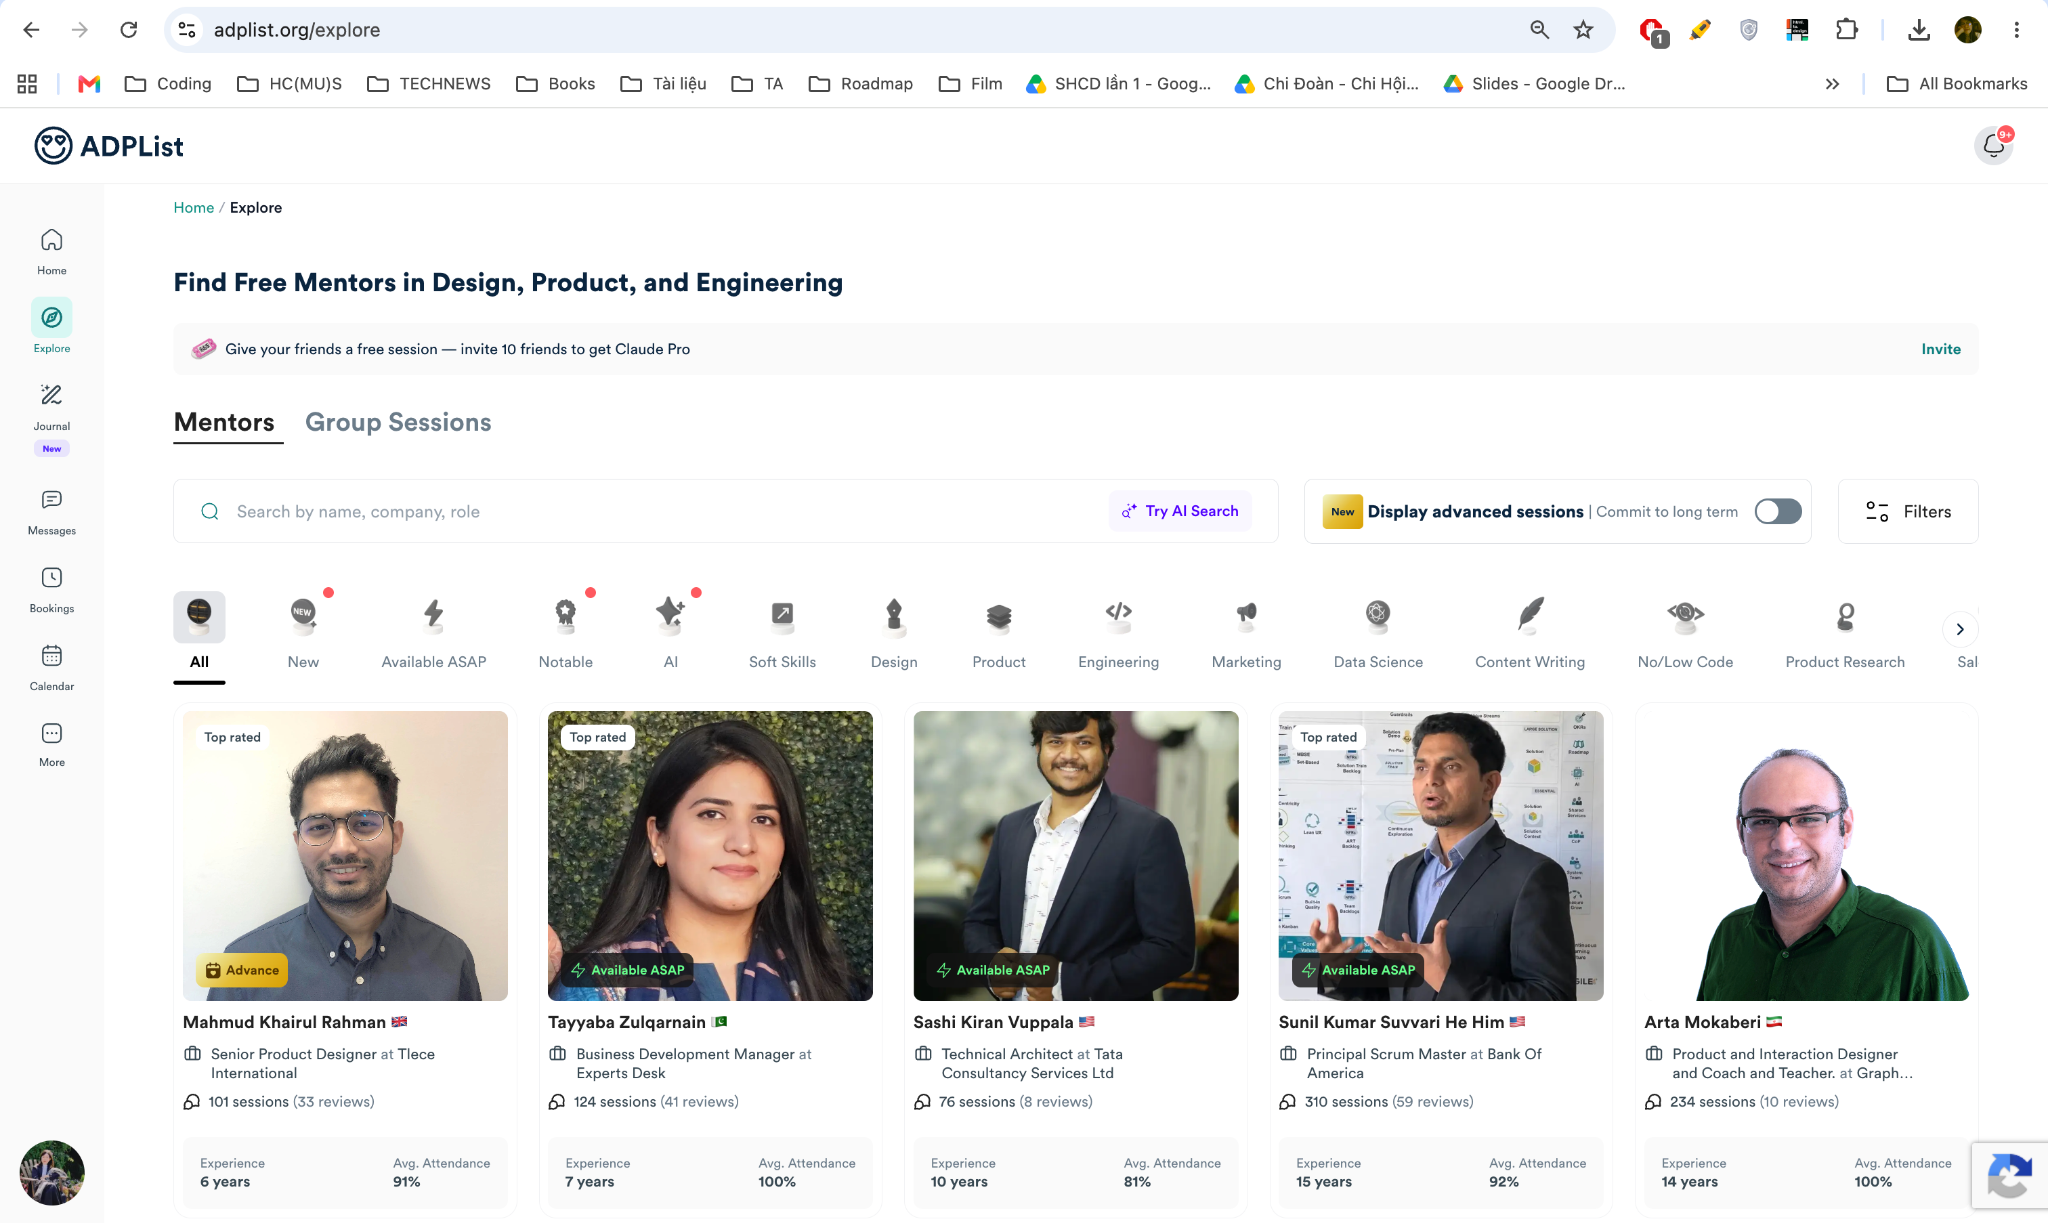
\includegraphics[width=0.90\textwidth,keepaspectratio]{hinh-2-3_adplist}
\caption{Giao diện nền tảng ADPList}
\label{fig:adplist}
\end{figure}

Tại Việt Nam, mô hình này vận hành sôi nổi qua nhiều nền tảng và cộng đồng nghề nghiệp. Tiêu biểu trong số đó là Mentori.vn (Hình \ref{fig:mentori}), với luồng nghiệp vụ tổ chức rất sát với định hướng mà nhóm hướng tới. Hệ thống AlumVerse tham khảo trải nghiệm người dùng diện rộng từ ADPList và bám sát mô hình luồng nghiệp vụ của Mentori.vn.

\begin{figure}[H]\centering
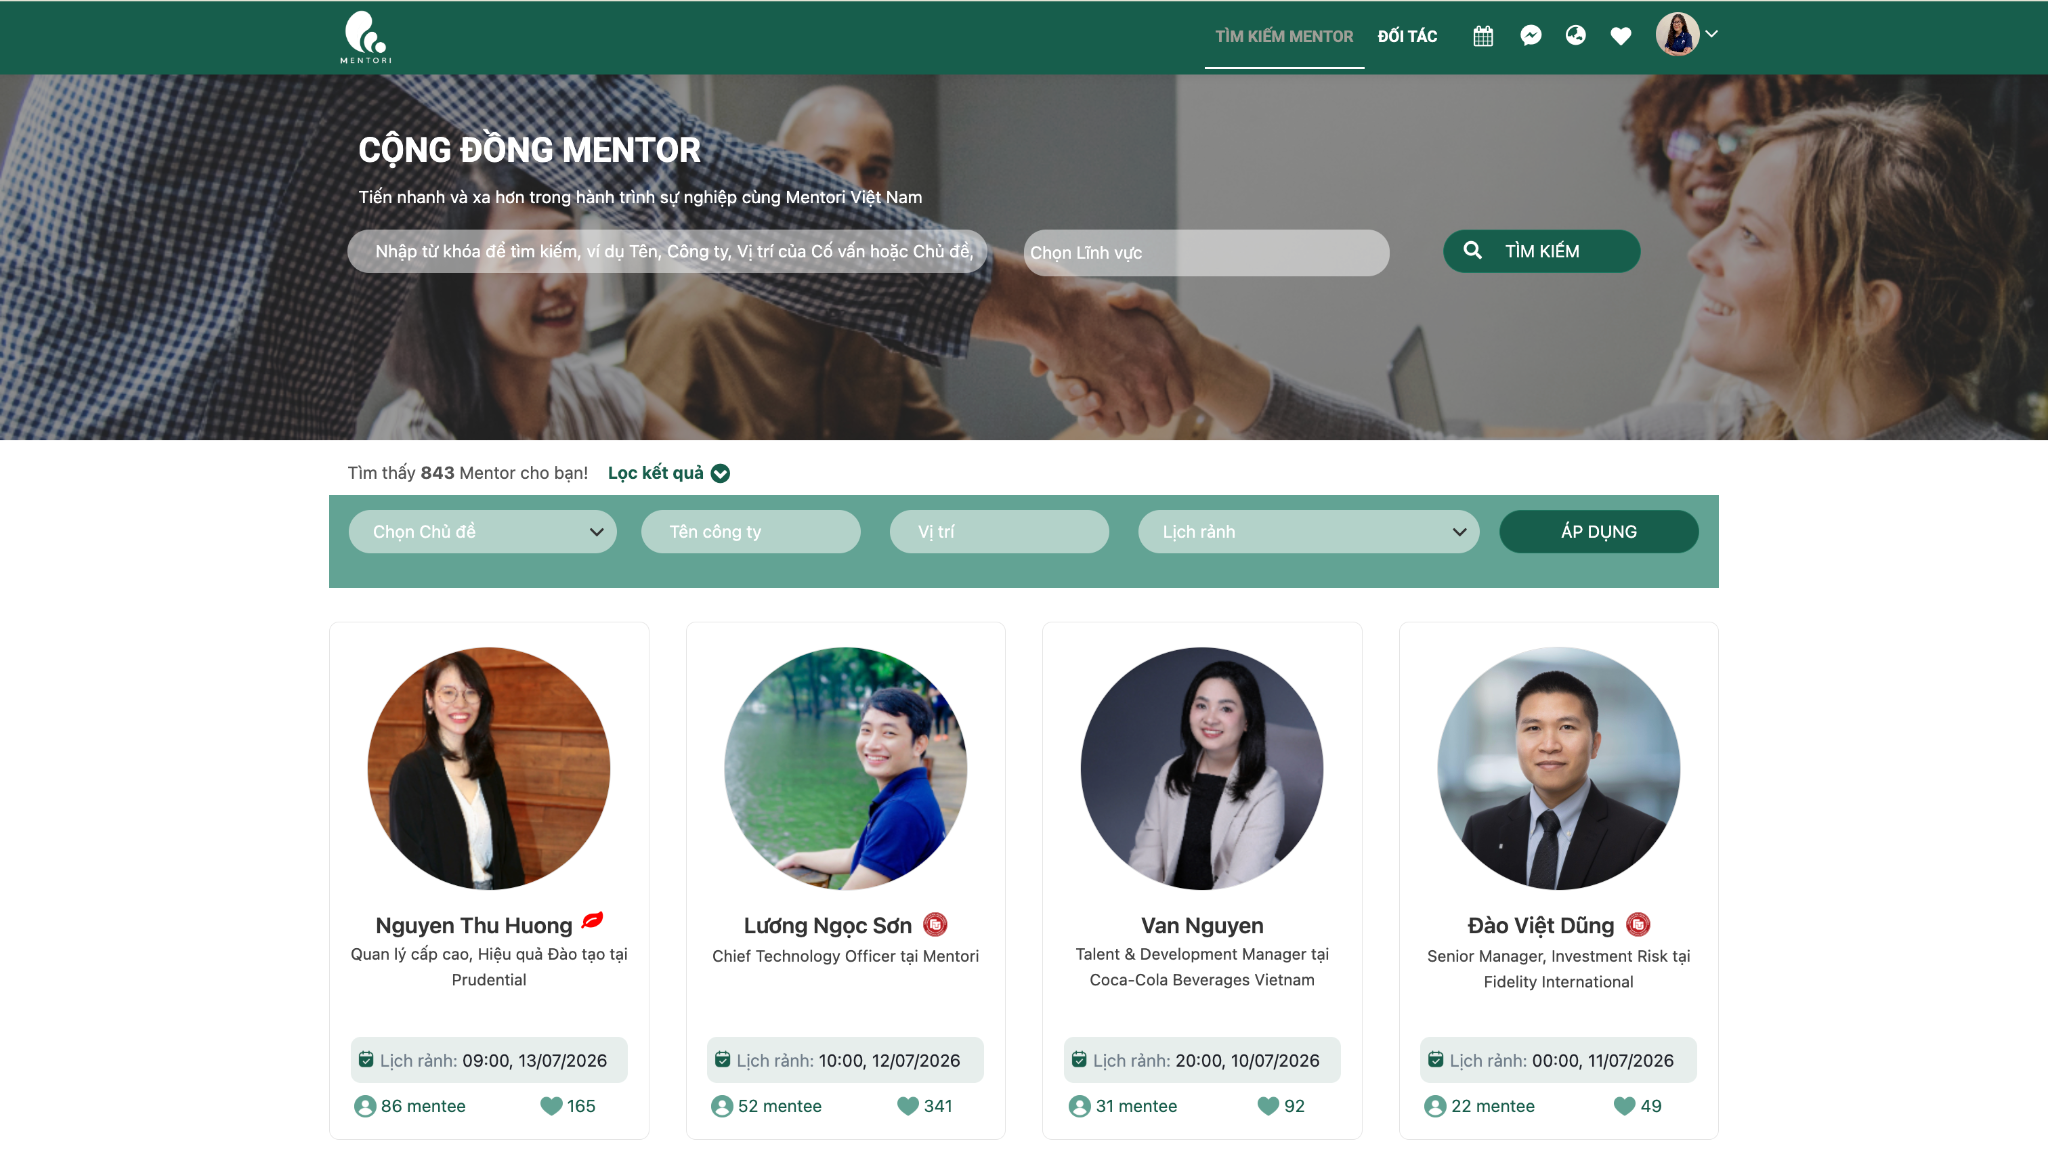
\includegraphics[width=0.90\textwidth,keepaspectratio]{hinh-2-4_mentori}
\caption{Giao diện nền tảng Mentori.vn}
\label{fig:mentori}
\end{figure}

Khoảng trống kỹ năng hiện nay càng làm bộc lộ rõ nhu cầu được cố vấn. Một khảo sát trên 3.000 sinh viên cho thấy 42\% chưa có việc làm do không đáp ứng được yêu cầu tuyển dụng, và 61\% sinh viên đã đi làm vẫn tự nhận thấy sự thiếu hụt về kỹ năng chuyên môn \cite{skillgap}.

\subsection{Khảo sát nhu cầu tại Trường Đại học Khoa học Tự nhiên}

Để kiểm chứng các nhu cầu trên trong bối cảnh cụ thể của nhà trường, nhóm đã thực hiện một khảo sát trực tuyến với sinh viên và cựu sinh viên, thu được 90 phản hồi hợp lệ, trong đó có 55 sinh viên năm ba và năm tư, 19 sinh viên năm nhất và năm hai, cùng 16 cựu sinh viên. Do quy mô mẫu còn khiêm tốn và nghiêng về nhóm sinh viên, kết quả khảo sát được sử dụng như một khảo sát thăm dò định hướng, không nhằm mục đích suy rộng thống kê.

\renewcommand{\arraystretch}{1.25}
{\small
\begin{longtable}{|>{\raggedright\arraybackslash}p{7.4cm}|c|c|}
\caption{Mức độ quan tâm của người tham gia khảo sát theo từng nhóm nhu cầu (thang 1 đến 5)}\label{tab:survey}\\
\hline \textbf{Hạng mục nhu cầu (sinh viên năm 3--4, n = 55)} & \textbf{Điểm trung bình} & \textbf{Số rất quan tâm} \\ \hline
\endfirsthead
\multicolumn{3}{l}{\itshape\small (tiếp theo trang trước)}\\[2pt]
\hline \textbf{Hạng mục nhu cầu (sinh viên năm 3--4, n = 55)} & \textbf{Điểm trung bình} & \textbf{Số rất quan tâm} \\ \hline
\endhead
\hline \multicolumn{3}{r}{\itshape\small (còn tiếp)}\\
\endfoot
\hline
\endlastfoot
Tiếp cận cơ hội nghề nghiệp & 4,38 & 30 \\ \hline
Diễn đàn hỏi đáp theo chủ đề & 4,29 & 25 \\ \hline
Tìm người cố vấn trong ngành & 4,27 & 28 \\ \hline
Cơ hội học tập sau đại học & 4,11 & 22 \\ \hline
Trang thông tin quỹ và học bổng & 3,98 & 18 \\ \hline
Chia sẻ khóa học cho sinh viên & 3,93 & 16 \\ \hline
Sự kiện kết nối nghề nghiệp & 3,87 & 16 \\ \hline
Trợ lý ảo hỗ trợ thông tin trường và khoa & 3,84 & 17 \\ \hline
\end{longtable}
}
\renewcommand{\arraystretch}{1}

\begin{figure}[H]\centering
\begin{tikzpicture}
\begin{axis}[
 width=13cm,height=7.4cm,
 xbar, xmin=0, xmax=5,
 bar width=8pt,
 font=\footnotesize,
 xlabel={Điểm trung bình (thang 1 đến 5)},
 symbolic y coords={Trợ lý ảo thông tin,Sự kiện kết nối,Chia sẻ khóa học,Quỹ và học bổng,Học tập sau đại học,Tìm người cố vấn,Diễn đàn hỏi đáp,Cơ hội nghề nghiệp},
 ytick=data, y dir=reverse,
 nodes near coords, nodes near coords style={font=\scriptsize},
 enlarge y limits=0.08,
 grid=major, grid style={dashed,gray!30},
]
\addplot[fill=blue!45,draw=blue!60] coordinates {
 (4.38,Cơ hội nghề nghiệp) (4.29,Diễn đàn hỏi đáp) (4.27,Tìm người cố vấn)
 (4.11,Học tập sau đại học) (3.98,Quỹ và học bổng) (3.93,Chia sẻ khóa học)
 (3.87,Sự kiện kết nối) (3.84,Trợ lý ảo thông tin)};
\end{axis}
\end{tikzpicture}
\caption{Mức độ quan tâm của sinh viên năm ba và năm tư theo các hạng mục (n = 55)}
\label{fig:surveychart}
\end{figure}

Ở nhóm sinh viên năm ba và năm tư, hai hạng mục được quan tâm nhất là tiếp cận cơ hội nghề nghiệp và tìm kiếm người cố vấn trong ngành; khoảng 85\% sinh viên nhóm này mong muốn tham gia hoạt động cố vấn. Kết quả này thống nhất với các phân tích lý thuyết ở những mục trước.

Một điểm đáng chú ý là sự lệch pha giữa cung và cầu: nhu cầu được cố vấn của sinh viên rất cao, nhưng phần lớn cựu sinh viên còn dè dặt khi được hỏi về khả năng đảm nhận vai trò người cố vấn. Nhận xét này là căn cứ trực tiếp để thiết kế các tính năng làm giảm rào cản cho người cố vấn, cụ thể là cho phép lưu nháp hồ sơ, tự động gợi ý thẻ kỹ năng và quản lý lịch linh hoạt. Tương tự, về xác minh danh tính, người tham gia có xu hướng dè dặt khi phải cung cấp giấy tờ tùy thân, do đó hệ thống thiết kế quy trình xác minh cho phép che bớt thông tin nhạy cảm trên giấy tờ.

\section{Khảo sát các hệ thống liên quan}

\subsection{Các nền tảng cựu sinh viên}

Kế thừa quá trình khảo sát của báo cáo AlumVerse 2024, nhóm xem xét một số nền tảng kết nối cựu sinh viên tiêu biểu. Hệ thống BKA Alumni của Trường Đại học Bách khoa Thành phố Hồ Chí Minh có nhiều tính năng tương tác kiểu mạng xã hội nhưng thiếu mục vinh danh cựu sinh viên tiêu biểu. Hệ thống RMIT Vietnam Alumni cho phép đăng ký sự kiện và có mục tư vấn, nhưng chỉ phát triển trên nền web và hạn chế tương tác giữa các cựu sinh viên. Hệ thống IoBM Alumni có tính năng tìm việc và tạo câu chuyện, nhưng thiếu mục tin tức và vinh danh. Hệ thống Oxford Alumni cho phép đăng ký sự kiện và tham gia nhiều nhóm, nhưng cũng chỉ phát triển trên nền web và hạn chế trao đổi giữa các thành viên.

Điểm chung của các nền tảng này là mạnh về truyền thông một chiều và quản lý sự kiện, nhưng yếu ở các luồng tạo giá trị hai chiều giữa cựu sinh viên và sinh viên.

\subsection{Ánh xạ tính năng với nền tảng tham khảo và vai trò cựu sinh viên}

Mỗi nhóm tính năng mở rộng của AlumVerse đều được nghiên cứu và tinh chỉnh từ một hoặc nhiều nền tảng thực tế, đồng thời được đối chiếu ngược lại với bảy vai trò của cựu sinh viên đã nêu ở mục 2.2. Bảng \ref{tab:mapping} tổng hợp toàn bộ phép ánh xạ này.

Về cố vấn, nhóm tham khảo luồng nghiệp vụ từ Mentori.vn và ADPList; các chu trình đăng ký hồ sơ, ghép cặp, đặt lịch hẹn và đánh giá phản hồi được thiết kế bám sát Mentori.vn. Về gây quỹ, thiết kế trang chiến dịch và cơ chế minh bạch lịch sử đóng góp được tham chiếu từ UEH Alumni và GlobalGiving. Về diễn đàn nghề nghiệp, cấu trúc phân tầng chuyên mục được học hỏi từ các cộng đồng chuyên môn và nền tảng hỏi đáp học thuật. Về sự kiện và hội viên, quy trình phát hành vé và cấp phát quyền lợi lấy cảm hứng từ RMIT Active Hub cùng các hệ thống phân phối vé điện tử phổ biến. Về cơ hội học tập và việc làm, cấu trúc bài đăng tuyển dụng và quản lý khóa học được xây dựng dựa trên các cổng việc làm và hệ thống quản lý học liệu trực tuyến.

\begin{figure}[H]\centering
\begin{subfigure}{0.46\textwidth}\centering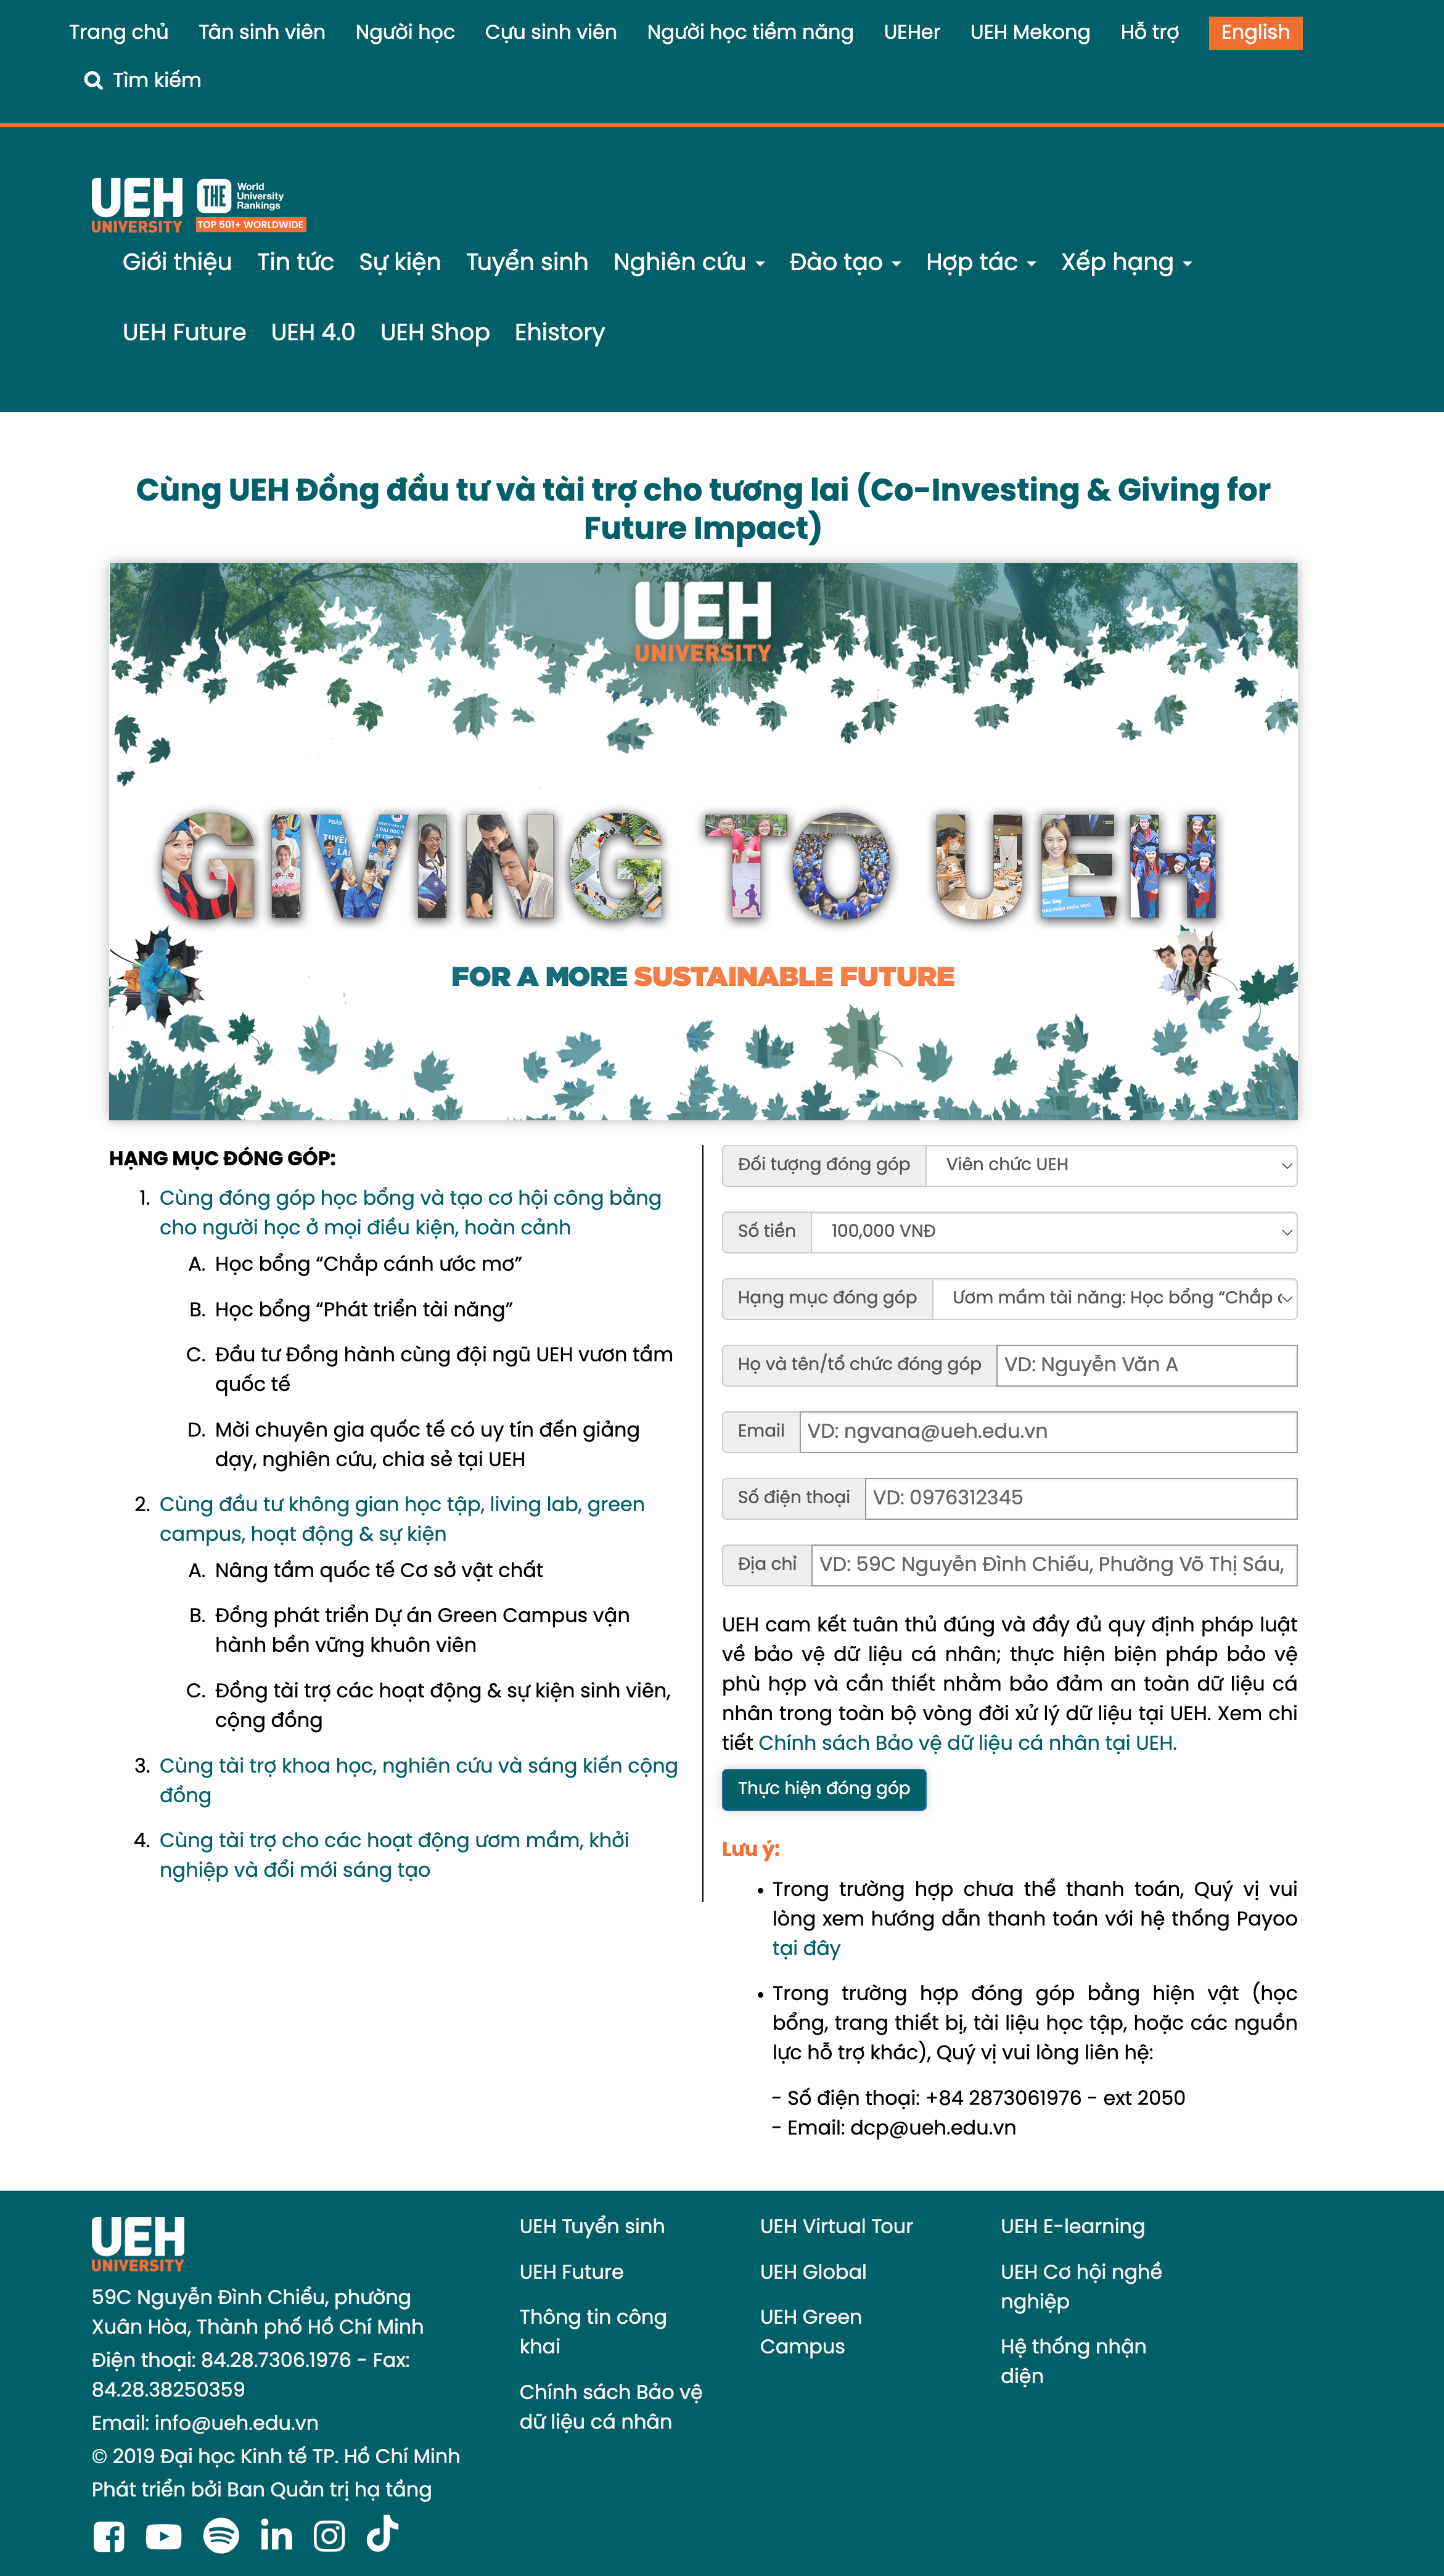
\includegraphics[width=\linewidth]{ref-gayquy-ueh}\caption{Trang gây quỹ tham chiếu}\end{subfigure}\hfill
\begin{subfigure}{0.46\textwidth}\centering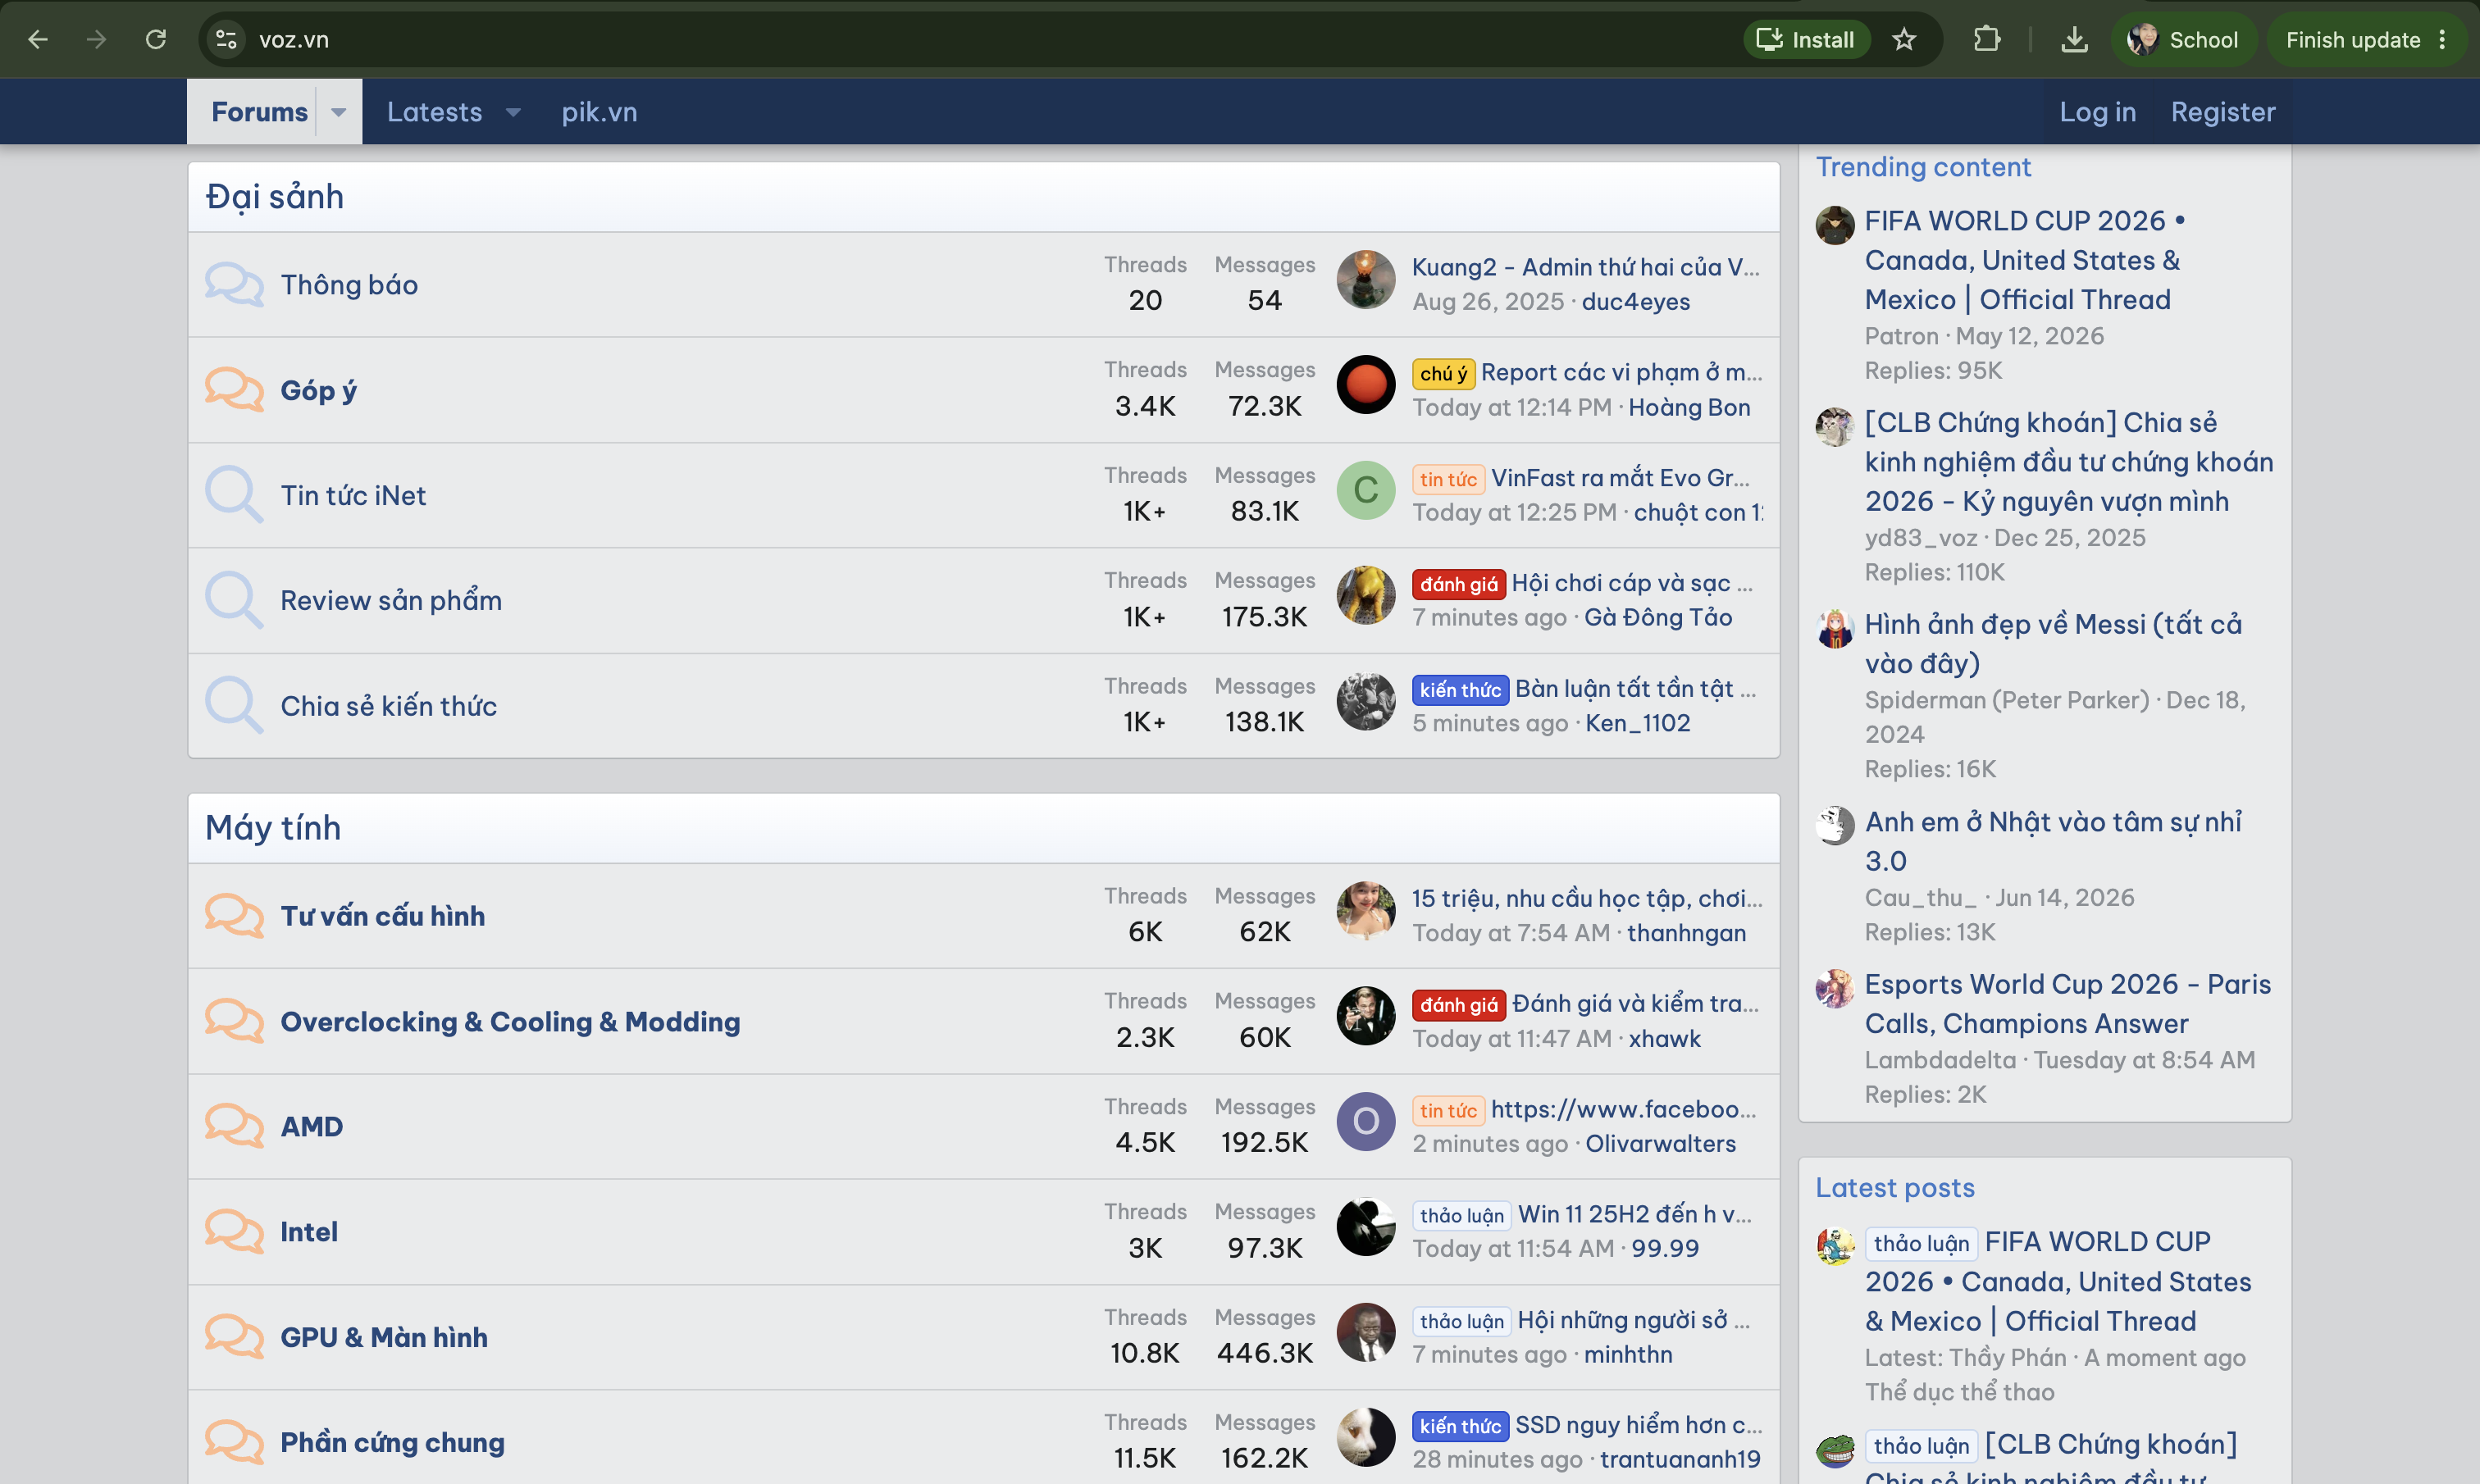
\includegraphics[width=\linewidth]{ref-diendan-voz}\caption{Diễn đàn tham chiếu}\end{subfigure}
\vspace{6pt}
\begin{subfigure}{0.46\textwidth}\centering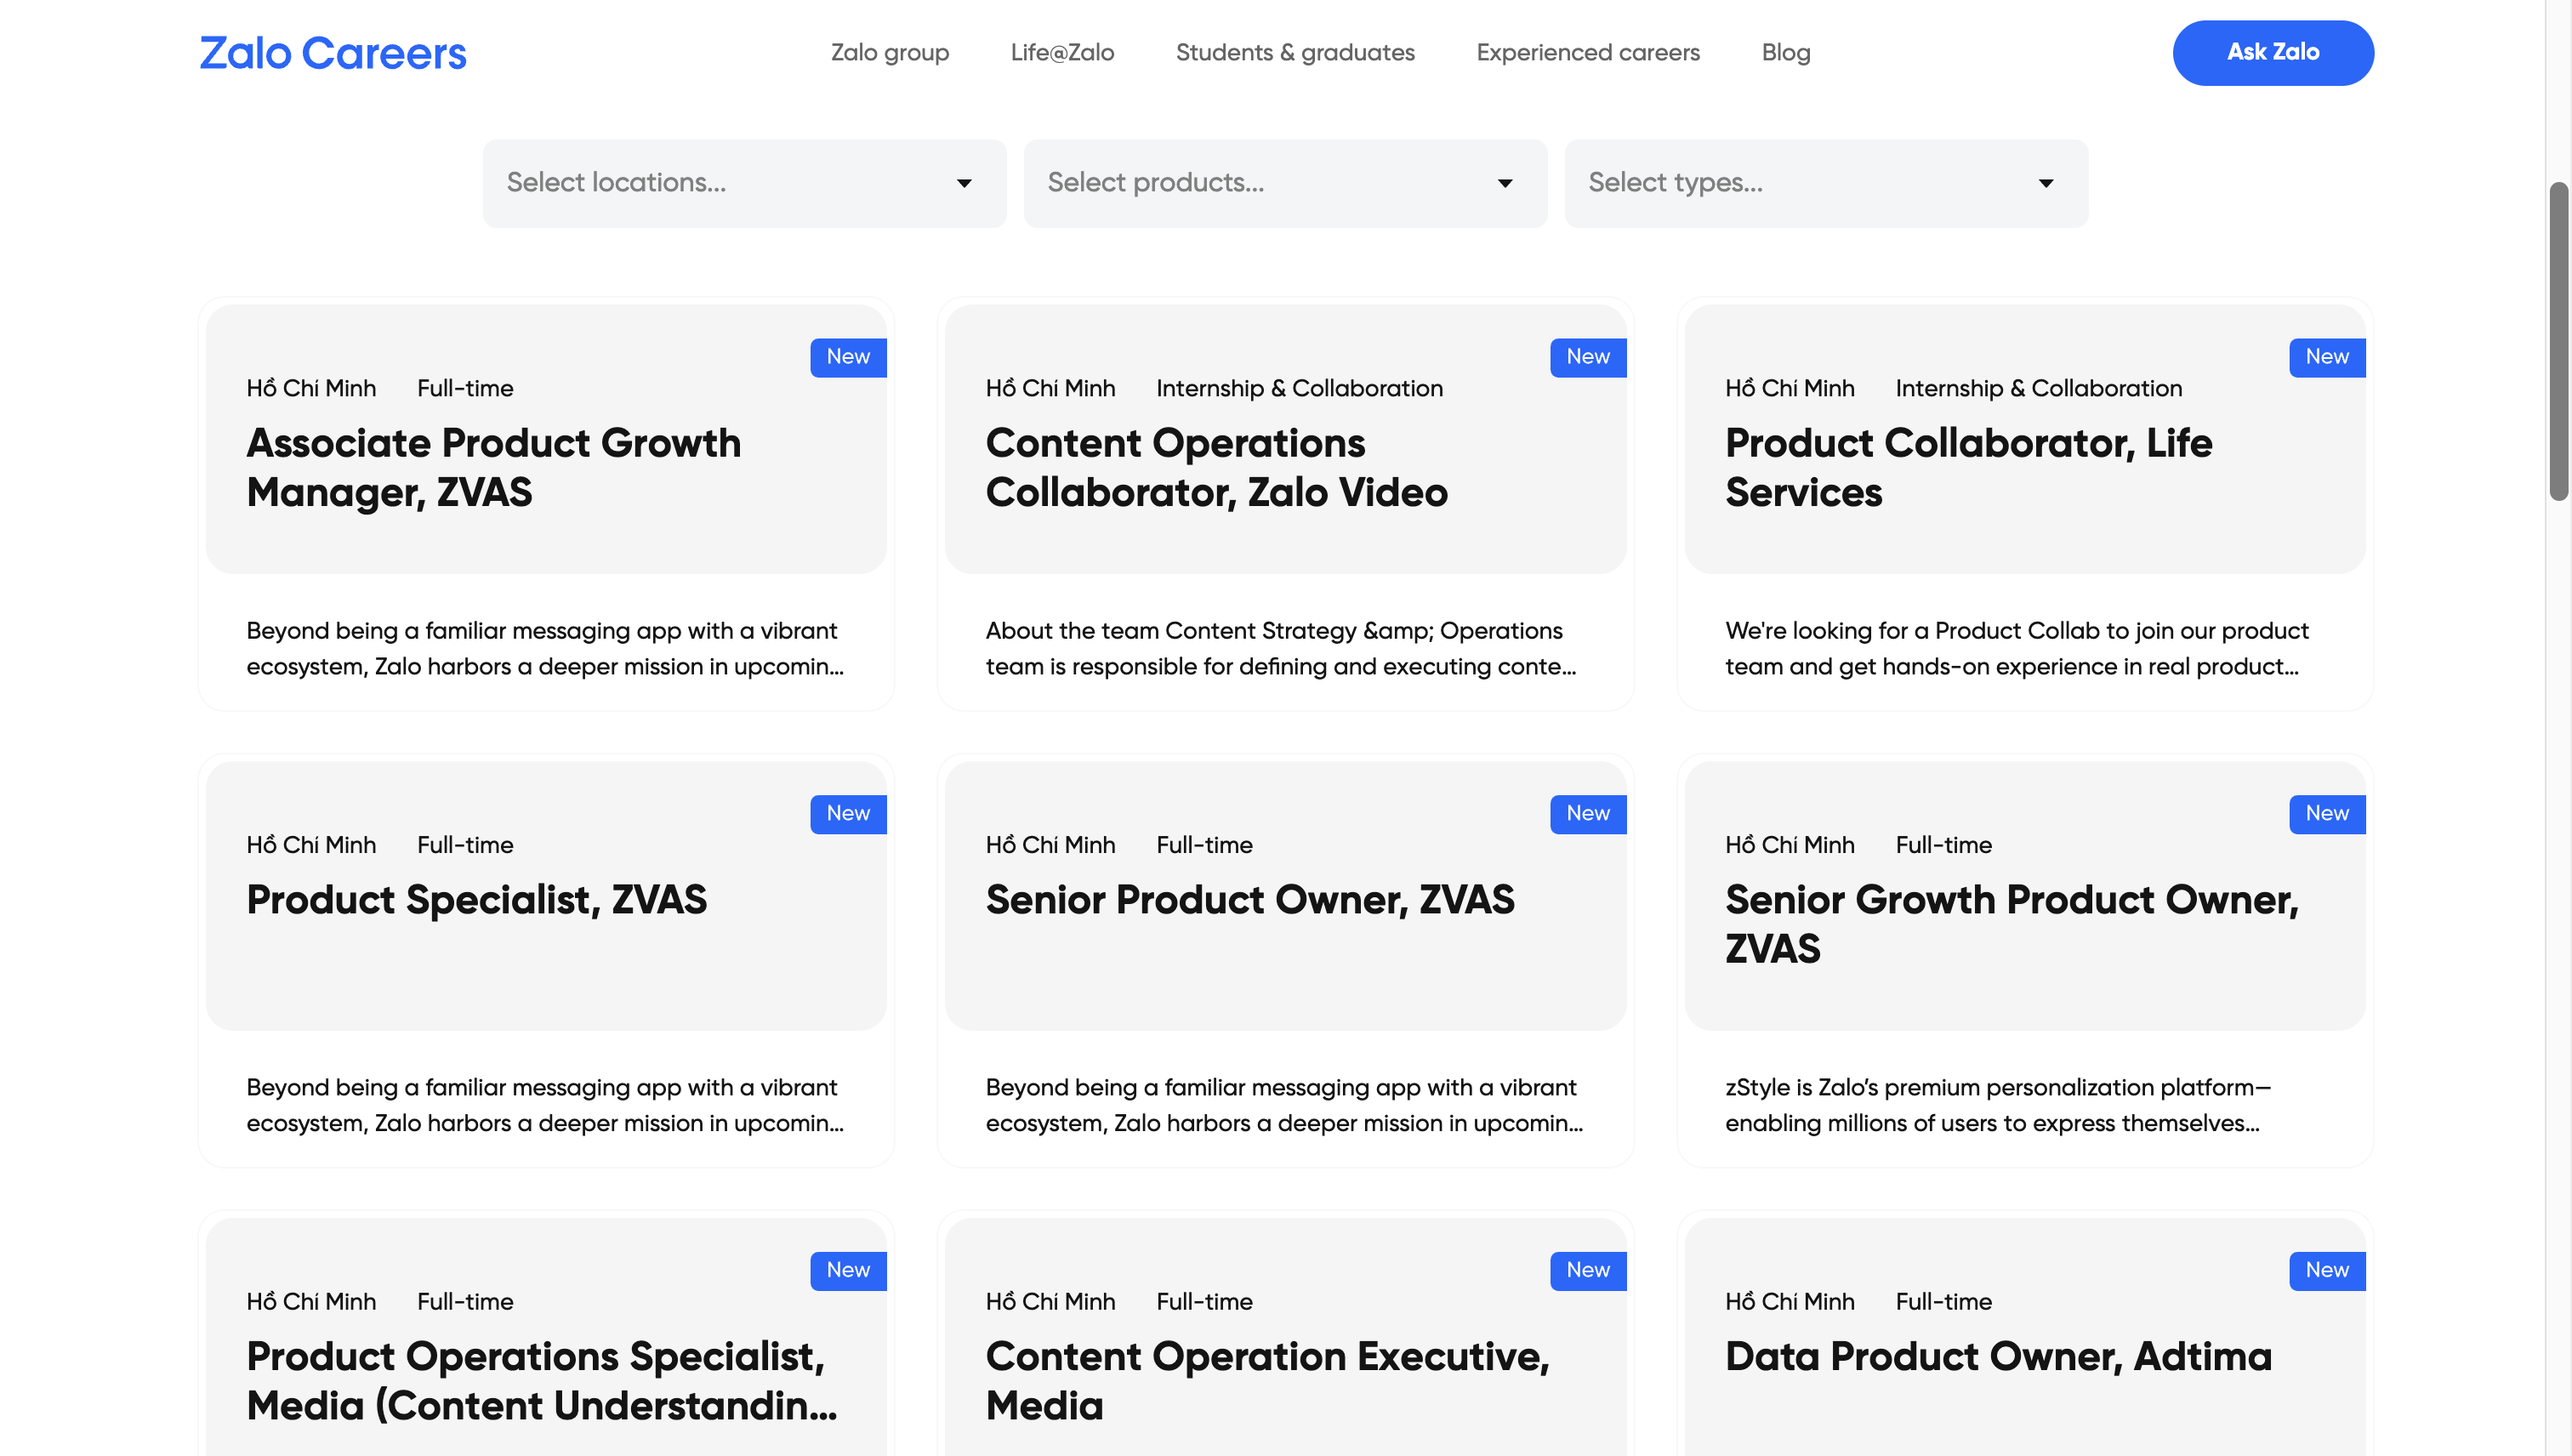
\includegraphics[width=\linewidth]{ref-vieclam-zalo}\caption{Cổng việc làm tham chiếu}\end{subfigure}
\caption{Một số nền tảng tham chiếu cho các nhóm tính năng gây quỹ, diễn đàn và việc làm}
\label{fig:refplatforms}
\end{figure}

\renewcommand{\arraystretch}{1.2}
\begin{longtable}{|>{\raggedright\arraybackslash}p{2.9cm}|>{\raggedright\arraybackslash}p{3.3cm}|>{\raggedright\arraybackslash}p{4.4cm}|>{\raggedright\arraybackslash}p{4.0cm}|}
\caption{Ánh xạ các nhóm tính năng của AlumVerse với nền tảng tham chiếu và vai trò cựu sinh viên}\label{tab:mapping}\\
\hline \textbf{Nhóm tính năng} & \textbf{Nền tảng tham chiếu} & \textbf{Yếu tố kế thừa} & \textbf{Vai trò được phục vụ} \\ \hline
\endfirsthead
\hline \textbf{Nhóm tính năng} & \textbf{Nền tảng tham chiếu} & \textbf{Yếu tố kế thừa} & \textbf{Vai trò được phục vụ} \\ \hline
\endhead
Cố vấn & Mentori.vn, ADPList & Chu trình đăng ký hồ sơ, ghép cặp theo kỹ năng, đặt lịch, đánh giá sau buổi & Cố vấn nghề nghiệp; hỗ trợ thế hệ sau \\ \hline
Gây quỹ & UEH Alumni, GlobalGiving & Trang chiến dịch, minh bạch lịch sử đóng góp, mục tiêu và tiến độ & Đóng góp tài chính cho nhà trường \\ \hline
Diễn đàn nghề nghiệp & Cộng đồng chuyên môn trực tuyến & Cấu trúc phân tầng chuyên mục, bình chọn và kiểm duyệt & Chia sẻ chuyên môn; giải đáp cho sinh viên \\ \hline
Sự kiện và hội viên & RMIT Active Hub, hệ thống vé điện tử & Quy trình đăng ký, phát hành vé, cấp phát quyền lợi & Gắn kết cộng đồng; xây dựng uy tín \\ \hline
Việc làm và học liệu & Cổng việc làm, hệ thống học liệu & Cấu trúc bài đăng tuyển dụng, phân loại khóa học & Giới thiệu việc làm; tham gia tuyển dụng \\ \hline
Vinh danh thành tích & Nền tảng cựu sinh viên tiêu biểu & Hồ sơ chân dung, câu chuyện nghề nghiệp & Hình mẫu truyền cảm hứng \\ \hline
\end{longtable}
\renewcommand{\arraystretch}{1}

\subsection{Mô hình mạng xã hội thuần túy và mô hình hướng giá trị}

Một đặc điểm chung của các nền tảng vận hành theo hướng mạng xã hội là tỉ lệ tương tác thực chất trên mỗi bài đăng rất thấp so với quy mô thành viên. Bảng \ref{tab:engagement} tổng hợp quan sát của nhóm về một số cộng đồng cựu sinh viên, cho thấy tỉ lệ tương tác ước lượng chỉ dao động trong một khoảng rất nhỏ. Cần lưu ý đây là số liệu quan sát của các cộng đồng khác, được dùng để minh họa cho xu hướng chung của mô hình mạng xã hội, không phải số liệu của riêng AlumVerse.

\renewcommand{\arraystretch}{1.25}
{\small
\begin{longtable}{|>{\raggedright\arraybackslash}p{6.4cm}|r|r|r|}
\caption{Tỉ lệ tương tác ước lượng của một số cộng đồng cựu sinh viên}\label{tab:engagement}\\
\hline \textbf{Cộng đồng} & \textbf{Thành viên} & \textbf{Tương tác TB} & \textbf{Tỉ lệ} \\ \hline
\endfirsthead
\multicolumn{4}{l}{\itshape\small (tiếp theo trang trước)}\\[2pt]
\hline \textbf{Cộng đồng} & \textbf{Thành viên} & \textbf{Tương tác TB} & \textbf{Tỉ lệ} \\ \hline
\endhead
\hline \multicolumn{4}{r}{\itshape\small (còn tiếp)}\\
\endfoot
\hline
\endlastfoot
Cựu SV và SV Đại học Sư phạm Kỹ thuật & 138.000 & 5--18 & 0,009--0,013\% \\ \hline
UEH Alumni & 9.600 & 12 & 0,12\% \\ \hline
Cựu SV Đại học Luật & 6.100 & 8 & 0,13\% \\ \hline
Cựu SV Đại học Kiến trúc & 15.000 & 23 & 0,15\% \\ \hline
Cựu SV Khoa Khoa học và Công nghệ Vật liệu & 2.700 & 9 & 0,33\% \\ \hline
\end{longtable}
}
\renewcommand{\arraystretch}{1}

Từ quan sát này, nhóm rút ra một nguyên tắc thiết kế cốt lõi cho AlumVerse: thay vì đặt mục tiêu tạo ra lượng tương tác thường xuyên như mạng xã hội, hệ thống tập trung vào những giá trị thiết thực có ích ngay cả khi người dùng chỉ truy cập không thường xuyên, chẳng hạn đặt lịch cố vấn, tìm kiếm cơ hội việc làm hay đóng góp cho một quỹ học bổng.

Theo nguyên tắc này, các tính năng mang tính tương tác như nhắn tin và diễn đàn không phải là mục đích cuối cùng của hệ thống, mà đóng vai trò công cụ hỗ trợ cho hoạt động cố vấn và kết nối nghề nghiệp. Để nhắn tin riêng, người dùng cần được chấp nhận yêu cầu kết nối trước. Diễn đàn được tổ chức theo chủ đề nghề nghiệp và học tập thay vì là một dòng thời gian tự do. Cách giới hạn có chủ đích này phân biệt AlumVerse với một mạng xã hội công cộng, và giữ cho các tính năng tương tác luôn phục vụ mục tiêu tạo giá trị của hệ thống.

\section{Phân tích hệ thống AlumVerse 2024}

\subsection{Kiến trúc và công nghệ}

Theo báo cáo AlumVerse 2024, hệ thống được xây dựng theo kiến trúc Microservices, với phần backend gồm chín dịch vụ Spring Boot, đăng ký dịch vụ qua Eureka và định tuyến qua API Gateway. Phần web được phát triển bằng Next.js, phần di động bằng Flutter. Cơ sở dữ liệu sử dụng MySQL với Spring Data JPA; hình ảnh được lưu trên Google Cloud Storage và thông báo đẩy được gửi qua Firebase Cloud Messaging. Đây là điểm xuất phát kỹ thuật để đối chiếu với các quyết định tái thiết kế của phiên bản 2026.

\begin{figure}[H]\centering
\begin{tikzpicture}[font=\footnotesize,
 box/.style={draw,rounded corners=2pt,align=center,inner sep=3pt},
 svc/.style={box,fill=red!8,minimum height=6mm,minimum width=20mm},
 ar/.style={-{Latex[length=2mm]},thick}]
\node[box,fill=blue!8,minimum width=26mm] (w) {Web (Next.js)};
\node[box,fill=blue!8,right=10mm of w,minimum width=26mm] (m) {Mobile (Flutter)};
\node[box,fill=gray!12,below=8mm of $(w)!0.5!(m)$,minimum width=44mm] (gw) {API Gateway};
\node[box,fill=yellow!14,right=16mm of gw,align=center] (eu) {Eureka\\ (service registry)};
\node[svc,below=20mm of gw.south west,anchor=north west] (s1) {Dịch vụ 1};
\node[svc,right=3mm of s1] (s2) {Dịch vụ 2};
\node[svc,right=3mm of s2] (s3) {\ldots};
\node[svc,right=3mm of s3] (s4) {Dịch vụ 9};
\begin{scope}[on background layer]
\node[draw,dashed,rounded corners,fill=red!3,fit={(s1) (s4)},inner sep=3mm] (grp) {};
\end{scope}
\node[font=\footnotesize\bfseries,anchor=south east] at ([yshift=1.5mm]grp.north east)
 {Chín dịch vụ Spring Boot độc lập};
\node[cylinder,shape border rotate=90,draw,fill=gray!12,minimum height=8mm,minimum width=22mm,
 below=9mm of grp] (db) {MySQL};
\draw[ar] (w) -- (gw); \draw[ar] (m) -- (gw);
\draw[ar] (gw.south) -- ([xshift=-32mm]grp.north);
\draw[ar,dashed] (eu.south) -- ([xshift=32mm]grp.north);
\draw[ar,dashed] (gw) -- (eu);
\draw[ar] (grp) -- (db);
\end{tikzpicture}
\caption{Sơ đồ tổng quan kiến trúc Microservices của hệ thống AlumVerse 2024}
\label{fig:arch2024}
\end{figure}

\renewcommand{\arraystretch}{1.25}
{\small
\begin{longtable}{|>{\raggedright\arraybackslash}p{3.6cm}|>{\raggedright\arraybackslash}p{4.9cm}|>{\raggedright\arraybackslash}p{4.9cm}|}
\caption{So sánh kiến trúc và công nghệ giữa AlumVerse 2024 và phiên bản 2026}\label{tab:compare2024}\\
\hline \textbf{Hạng mục} & \textbf{AlumVerse 2024} & \textbf{AlumVerse 2026} \\ \hline
\endfirsthead
\multicolumn{3}{l}{\itshape\small (tiếp theo trang trước)}\\[2pt]
\hline \textbf{Hạng mục} & \textbf{AlumVerse 2024} & \textbf{AlumVerse 2026} \\ \hline
\endhead
\hline \multicolumn{3}{r}{\itshape\small (còn tiếp)}\\
\endfoot
\hline
\endlastfoot
Kiến trúc & Microservices, chín dịch vụ & Modular Monolith kết hợp Layered \\ \hline
Điều phối dịch vụ & Eureka và API Gateway & Không cần, một ứng dụng duy nhất \\ \hline
Mô hình xử lý & Đồng bộ, chặn luồng & Bất đồng bộ, không chặn luồng \\ \hline
Framework backend & Spring Boot với Spring MVC & Spring Boot với Spring WebFlux \\ \hline
Truy cập dữ liệu & Spring Data JPA & R2DBC \\ \hline
Cơ sở dữ liệu & MySQL & PostgreSQL \\ \hline
Đa đơn vị & Không hỗ trợ & Chia sẻ cơ sở dữ liệu theo \texttt{organization\_id} \\ \hline
Ứng dụng web & Next.js & React với Vite \\ \hline
Ứng dụng di động & Flutter & Flutter \\ \hline
Lưu trữ tệp & Google Cloud Storage & Lưu trữ nội bộ qua Nginx \\ \hline
Thông báo & Firebase Cloud Messaging & Thông báo trong ứng dụng và đẩy thời gian thực \\ \hline
Kiểm thử tự động & Chưa triển khai & 215 hàm kiểm thử tầng nghiệp vụ \\ \hline
\end{longtable}
}
\renewcommand{\arraystretch}{1}

\subsection{Phạm vi chức năng và mô hình dữ liệu}

Bảng so sánh chức năng trong báo cáo 2024 liệt kê chín tính năng cốt lõi, gồm hỗ trợ đa nền tảng, quản lý vai trò và phân quyền, đăng ký tham gia sự kiện, gương thành công, tư vấn và cố vấn, tạo nhóm, đăng bài trong nhóm, nhắn tin và tìm kiếm cựu sinh viên. Toàn bộ các tính năng này thuộc nhóm nội dung và kết nối xã hội, chưa có tính năng nào tạo ra giá trị nghề nghiệp hay tài chính đo lường được. Riêng tính năng tư vấn và cố vấn của bản 2024 mới chỉ ở mức một bài đăng kèm bình chọn ý kiến và bình luận, chưa có cơ chế đặt lịch hẹn hay theo dõi tiến độ như một chương trình cố vấn có cấu trúc.

Về dữ liệu, lược đồ của hệ thống 2024 được tổ chức quanh tám nhóm thực thể, gồm người dùng, vai trò, tin tức, sự kiện, gương thành công, tư vấn, nhóm và nhắn tin. Không có nhóm bảng nào dành cho gây quỹ, việc làm, học liệu hay khảo sát, cho thấy hệ thống chưa được thiết kế để phục vụ các nhóm giá trị này.

\begin{figure}[H]\centering
\begin{tikzpicture}[font=\footnotesize,
 e/.style={draw,rounded corners=2pt,fill=red!7,minimum height=7mm,minimum width=24mm,align=center}]
\node[e] (a) at (0,0) {Người dùng};
\node[e] (b) at (3,0) {Vai trò};
\node[e] (c) at (6,0) {Tin tức};
\node[e] (d) at (9,0) {Sự kiện};
\node[e] (f) at (0,-1) {Gương thành công};
\node[e] (g) at (3,-1) {Tư vấn};
\node[e] (h) at (6,-1) {Nhóm};
\node[e] (i) at (9,-1) {Nhắn tin};
\begin{scope}[on background layer]
\node[draw,dashed,rounded corners,fill=red!2,fit={(a)(i)},inner sep=3.5mm] (bx) {};
\end{scope}
\node[font=\scriptsize\itshape,below=1mm of bx,text width=110mm,align=center]
 {Không có nhóm bảng nào cho gây quỹ, việc làm, học liệu hay khảo sát};
\end{tikzpicture}
\caption{Các nhóm thực thể trong lược đồ cơ sở dữ liệu của hệ thống AlumVerse 2024}
\label{fig:erd2024}
\end{figure}

\subsection{Nợ kỹ thuật và hạn chế vận hành}

Báo cáo 2024 ghi nhận một số hạn chế đáng chú ý về mặt vận hành. Thời gian phản hồi của máy chủ khi triển khai trực tuyến khá chậm, mất khoảng sáu giây cho mỗi lượt gọi lấy danh sách, một phần do khó khăn trong việc triển khai kiến trúc Microservices và do phải chọn khu vực máy chủ ở xa. Hệ thống cũng chưa kịp triển khai kiểm thử tự động, và mới chỉ hỗ trợ nhắn tin cá nhân, chưa có nhắn tin nhóm.

Những hạn chế này là động lực trực tiếp cho hai trụ cột tái thiết kế kỹ thuật và cải tiến nghiệp vụ của phiên bản 2026. Cần lưu ý rằng nhóm không tiếp nhận mã nguồn của phiên bản 2024, nên các số liệu nêu trên được trích dẫn từ báo cáo của khóa trước chứ không phải kết quả đo lại của nhóm.

\subsection{Tính năng kế thừa và loại bỏ có chủ đích}

Phiên bản 2026 kế thừa các luồng đã được kiểm chứng của bản 2024, như tin tức, sự kiện, nhắn tin và xác minh cựu sinh viên, đồng thời thực hiện một số thay đổi có chủ đích.

Tính năng nhóm cộng đồng kèm bài đăng của bản 2024 được thay bằng diễn đàn có cấu trúc kết hợp mạng lưới kết nối. Cơ chế tạo và chỉnh sửa vai trò linh hoạt qua giao diện được thay bằng tập vai trò cố định gắn với định danh tổ chức; ở quy mô một nền tảng cựu sinh viên, tệp người dùng là cố định nên đây là lựa chọn giúp giảm độ phức tạp và tăng tốc độ truy vấn, chứ không phải một thiếu sót về phạm vi. Cơ chế thông báo đẩy qua dịch vụ ngoài cũng được điều chỉnh thành thông báo trong ứng dụng.

\section{Khoảng trống và đề xuất định hướng giải pháp}

Tổng hợp từ phân tích nhu cầu người dùng, khảo sát các hệ thống liên quan và phân tích hiện trạng bản 2024, nhóm xác định bốn định hướng cho phiên bản 2026.

Thứ nhất, giữ lại và hoàn thiện các luồng nghiệp vụ đã được kiểm chứng.

Thứ hai, đơn giản hóa kiến trúc triển khai để giảm chi phí vận hành, thông qua việc chuyển sang kiến trúc Modular Monolith kết hợp Layered trên nền Reactive Programming.

Thứ ba, bổ sung các nhóm tính năng tạo giá trị thực, gồm cố vấn có cấu trúc, cơ hội học tập và việc làm, gây quỹ minh bạch, diễn đàn nghề nghiệp, khảo sát và thống kê việc làm, trợ lý ảo, cùng mô hình Multi-tenant cho phép mỗi đơn vị có một cổng kết nối riêng.

Thứ tư, chuẩn hóa danh mục tính năng để làm căn cứ thống nhất cho việc phân tích yêu cầu, phân công công việc và đánh giá mức độ hoàn thành.

Sau quá trình rà soát và hợp nhất, danh mục tính năng của phiên bản 2026 gồm 86 tính năng thuộc 15 module, trong đó 8 module kế thừa từ phiên bản 2024 và 7 module hoàn toàn mới. Danh sách đầy đủ kèm mô tả từng tính năng được trình bày ở Phụ lục A. Phần minh họa giao diện và chi tiết triển khai được trình bày trong Chương 3 và Chương 4, còn số liệu đánh giá mức độ hoàn thành được trình bày trong Chương 5.

Định hướng đơn giản hóa kiến trúc không chỉ dừng ở cách tổ chức mã nguồn, mà còn đi kèm các thực hành bảo đảm chất lượng như kiểm thử tự động cho tầng nghiệp vụ, tích hợp và triển khai liên tục, cùng giám sát vận hành. Các nội dung này được trình bày ở Chương 4 và Chương 5.

Nhìn tổng thể, AlumVerse ưu tiên tối đa hóa lợi ích thiết thực trong từng lần truy cập của người dùng thay vì cố gắng mô phỏng mức độ tương tác bề mặt của các nền tảng mạng xã hội đại chúng. Những định hướng chiến lược này đóng vai trò kim chỉ nam và sẽ được đặc tả thành các yêu cầu hệ thống chi tiết trong chương tiếp theo.

% ─────────────────────── CHƯƠNG 3 ───────────────────────
\chapter{PHÂN TÍCH YÊU CẦU VÀ THIẾT KẾ HỆ THỐNG}

Chương này trình bày quá trình phân tích yêu cầu và thiết kế hệ thống AlumVerse 2026, gồm mục tiêu hệ thống, đặc tả tác nhân và yêu cầu chức năng, kiến trúc nghiệp vụ đa tổ chức, thiết kế kiến trúc phần mềm, thiết kế cơ sở dữ liệu và thiết kế giao diện đa nền tảng.

\section{Phân tích yêu cầu}

\subsection{Mục tiêu hệ thống}

Bài toán mà hệ thống cần giải quyết là tạo ra một kênh kết nối giữa sinh viên, cựu sinh viên và nhà trường, trong đó mỗi lần truy cập của người dùng đều mang lại một giá trị cụ thể. Đây là điểm khác biệt căn bản so với cách tiếp cận mạng xã hội của phiên bản trước, vốn đòi hỏi người dùng phải quay lại thường xuyên mới tạo ra giá trị.

Đối tượng sử dụng gồm ba nhóm chính. Sinh viên đang theo học cần định hướng nghề nghiệp, tìm người cố vấn, tiếp cận cơ hội việc làm và học liệu. Cựu sinh viên cần kết nối lại với cộng đồng, tham gia sự kiện, đóng góp cho nhà trường và chia sẻ kinh nghiệm. Đội ngũ quản trị ở cấp khoa và cấp trường cần quản lý dữ liệu người dùng, kiểm duyệt nội dung, tổ chức sự kiện, vận hành các chiến dịch gây quỹ và thực hiện nghĩa vụ thống kê việc làm.

Về yêu cầu chức năng, hệ thống phải bao phủ đầy đủ các luồng nghiệp vụ đã kế thừa từ phiên bản 2024 đồng thời bổ sung các nhóm tính năng tạo giá trị mới. Về yêu cầu phi chức năng, hệ thống phải xử lý được nhiều kết nối đồng thời, cô lập dữ liệu giữa các đơn vị, bảo đảm an toàn ở mức xác thực và phân quyền, và duy trì khả năng bảo trì lâu dài.

\subsection{Đặc tả tác nhân}

Hệ thống phục vụ năm nhóm tác nhân với phạm vi quyền hạn khác nhau.

Khách vãng lai là người dùng chưa đăng nhập, chỉ xem được nội dung công khai như tin tức, giới thiệu khoa và danh sách sự kiện, đồng thời có thể thực hiện đăng ký hoặc đăng nhập.

Sinh viên là người dùng đã đăng nhập với vai trò đang theo học, có quyền quản lý hồ sơ cá nhân, tham gia diễn đàn, đăng ký sự kiện, gửi yêu cầu kết nối và nhắn tin, đăng ký làm người được cố vấn, và đóng góp cho các quỹ.

Cựu sinh viên có toàn bộ quyền của sinh viên, bổ sung thêm quyền đăng ký làm người cố vấn, đăng tin tuyển dụng, chia sẻ học liệu và tham gia xác minh chéo cho cựu sinh viên khác.

Quản trị viên cấp khoa quản lý toàn bộ nội dung và người dùng trong phạm vi khoa mình phụ trách, gồm kiểm duyệt bài viết, tổ chức sự kiện, duyệt hồ sơ cố vấn, xác minh danh tính và vận hành quỹ của khoa.

Quản trị viên cấp trường có phạm vi toàn hệ thống, bổ sung quyền khởi tạo và cấu hình đơn vị mới, cấp tài khoản quản trị khoa, quản lý mô hình AI và theo dõi giám sát vận hành.

Ở mức mã nguồn, hệ thống dùng một tập vai trò cố định kết hợp với cột định danh tổ chức để phân biệt phạm vi quản trị, thay cho cơ chế tạo và sửa vai trò linh hoạt của phiên bản 2024. Cách này giảm độ phức tạp và đủ dùng ở quy mô một nền tảng cựu sinh viên.

Quan hệ giữa năm tác nhân được mô hình hóa bằng quan hệ khái quát hóa của UML, trình bày ở Hình \ref{fig:ucactors}. Trên nhánh người dùng, Sinh viên kế thừa Khách vãng lai và Cựu sinh viên kế thừa Sinh viên; trên nhánh quản trị, Quản trị trường kế thừa Quản trị khoa. Nhờ quan hệ kế thừa, mỗi sơ đồ use case của một tác nhân chỉ cần trình bày phần use case bổ sung của riêng tác nhân đó, tránh lặp lại toàn bộ danh sách ở mọi sơ đồ.

Các Hình \ref{fig:ucguest} đến \ref{fig:ucsadmin2} trình bày sơ đồ use case tách riêng cho từng tác nhân, vẽ theo ký pháp UML với ranh giới hệ thống, nhóm use case theo phân hệ nghiệp vụ và các quan hệ $\ll$include$\gg$, $\ll$extend$\gg$.

Danh sách use case trong các sơ đồ này bao phủ toàn bộ danh mục 86 tính năng ở Phụ lục A theo nguyên tắc sau. Những tính năng cùng phục vụ một mục tiêu của người dùng được gộp thành một use case, ví dụ nhóm tính năng vé điện tử và xem vé của tôi. Ngược lại, bốn tính năng thuộc về hạ tầng chứ không phải mục tiêu mà tác nhân chủ động theo đuổi thì không xuất hiện dưới dạng use case, gồm phân quyền theo vai trò, ngữ cảnh đa đơn vị, dịch vụ lưu trữ và phục vụ tệp, và kênh sự kiện thời gian thực. Bốn tính năng này là điều kiện nền cho các use case khác và đã được mô tả ở mục 3.2.2 và Chương 4.

Do số lượng use case của một số tác nhân khá lớn, sơ đồ của tác nhân Sinh viên được tách làm ba hình và sơ đồ của tác nhân Quản trị viên cấp khoa được tách làm hai hình, nhằm giữ kích thước chữ trong sơ đồ đủ lớn để đọc trên bản in. Với hai tác nhân có quan hệ kế thừa là Cựu sinh viên và Quản trị viên cấp trường, sơ đồ chỉ trình bày phần use case bổ sung của riêng tác nhân đó; toàn bộ use case của tác nhân cha được kế thừa và không vẽ lại.

\renewcommand{\arraystretch}{1.2}
\begin{longtable}{|>{\raggedright\arraybackslash}p{3.0cm}|>{\raggedright\arraybackslash}p{5.2cm}|>{\raggedright\arraybackslash}p{6.3cm}|}
\caption{Đặc tả các tác nhân và phạm vi dữ liệu}\label{tab:actors}\\
\hline \textbf{Tác nhân} & \textbf{Phạm vi dữ liệu} & \textbf{Nhóm quyền tiêu biểu} \\ \hline
\endfirsthead
\hline \textbf{Tác nhân} & \textbf{Phạm vi dữ liệu} & \textbf{Nhóm quyền tiêu biểu} \\ \hline
\endhead
Khách vãng lai & Chỉ nội dung công khai & Xem tin tức, giới thiệu, sự kiện; đăng ký; đăng nhập \\ \hline
Sinh viên & Trong phạm vi tổ chức đang tham gia & Quản lý hồ sơ; diễn đàn; đăng ký sự kiện; yêu cầu kết nối và nhắn tin; đăng ký được cố vấn; đóng góp quỹ \\ \hline
Cựu sinh viên & Trong phạm vi tổ chức đang tham gia & Toàn bộ quyền của sinh viên; đăng ký làm người cố vấn; đăng tin tuyển dụng; chia sẻ học liệu; xác minh chéo \\ \hline
Quản trị khoa & Giới hạn theo định danh tổ chức của khoa & Kiểm duyệt nội dung; tổ chức sự kiện; duyệt hồ sơ cố vấn; xác minh danh tính; vận hành quỹ của khoa \\ \hline
Quản trị trường & Toàn hệ thống & Toàn bộ quyền quản trị khoa; khởi tạo và cấu hình đơn vị; cấp tài khoản quản trị; quản lý mô hình AI; giám sát vận hành \\ \hline
\end{longtable}
\renewcommand{\arraystretch}{1}

\begin{figure}[H]\centering
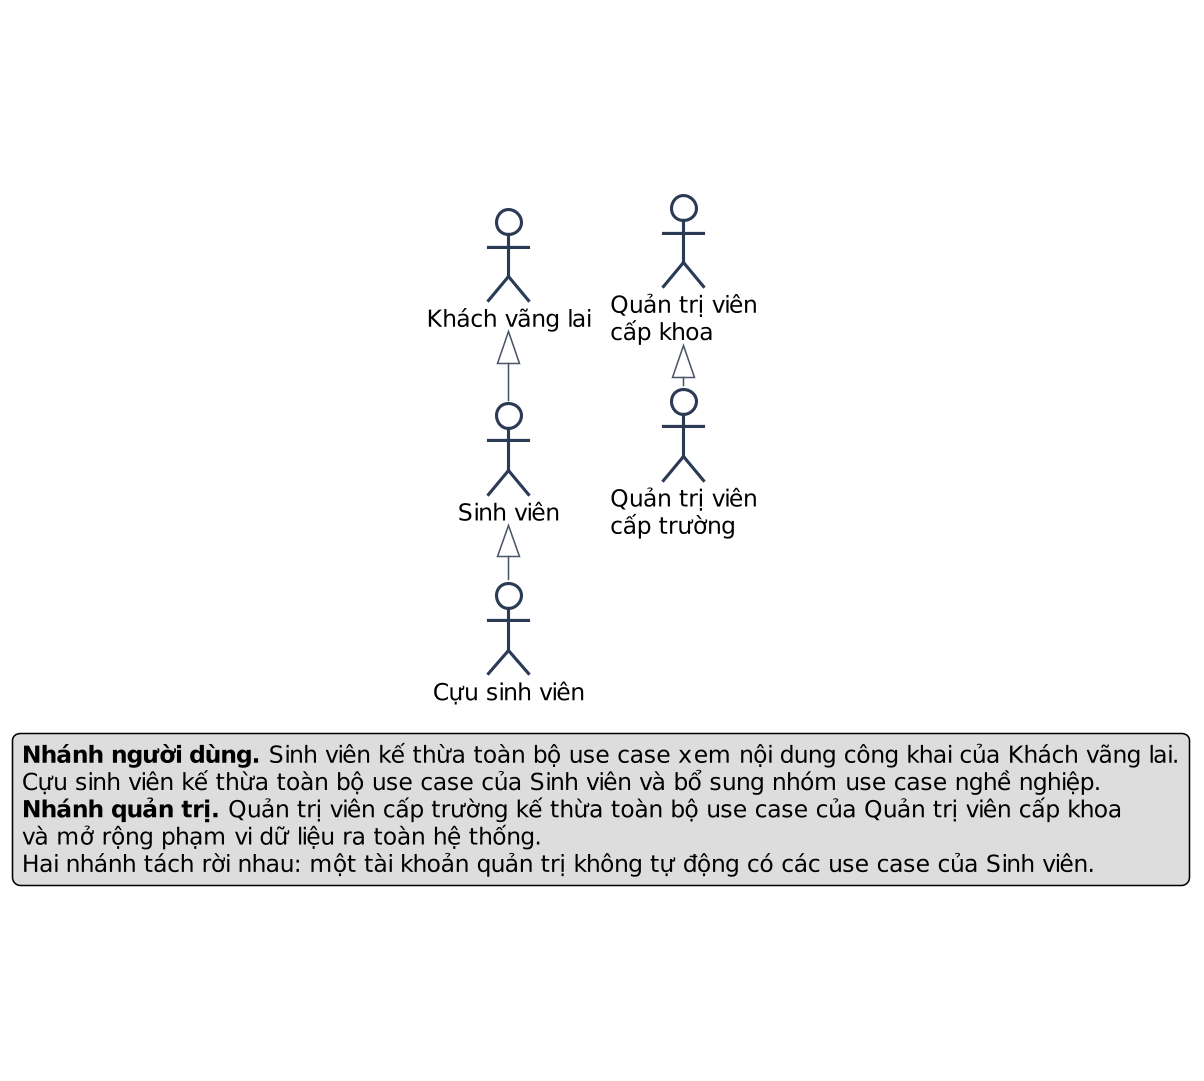
\includegraphics[width=\textwidth,height=0.84\textheight,keepaspectratio]{uc0-actors}
\caption{Quan hệ khái quát hóa giữa các tác nhân của hệ thống}
\label{fig:ucactors}
\end{figure}

\begin{figure}[H]\centering
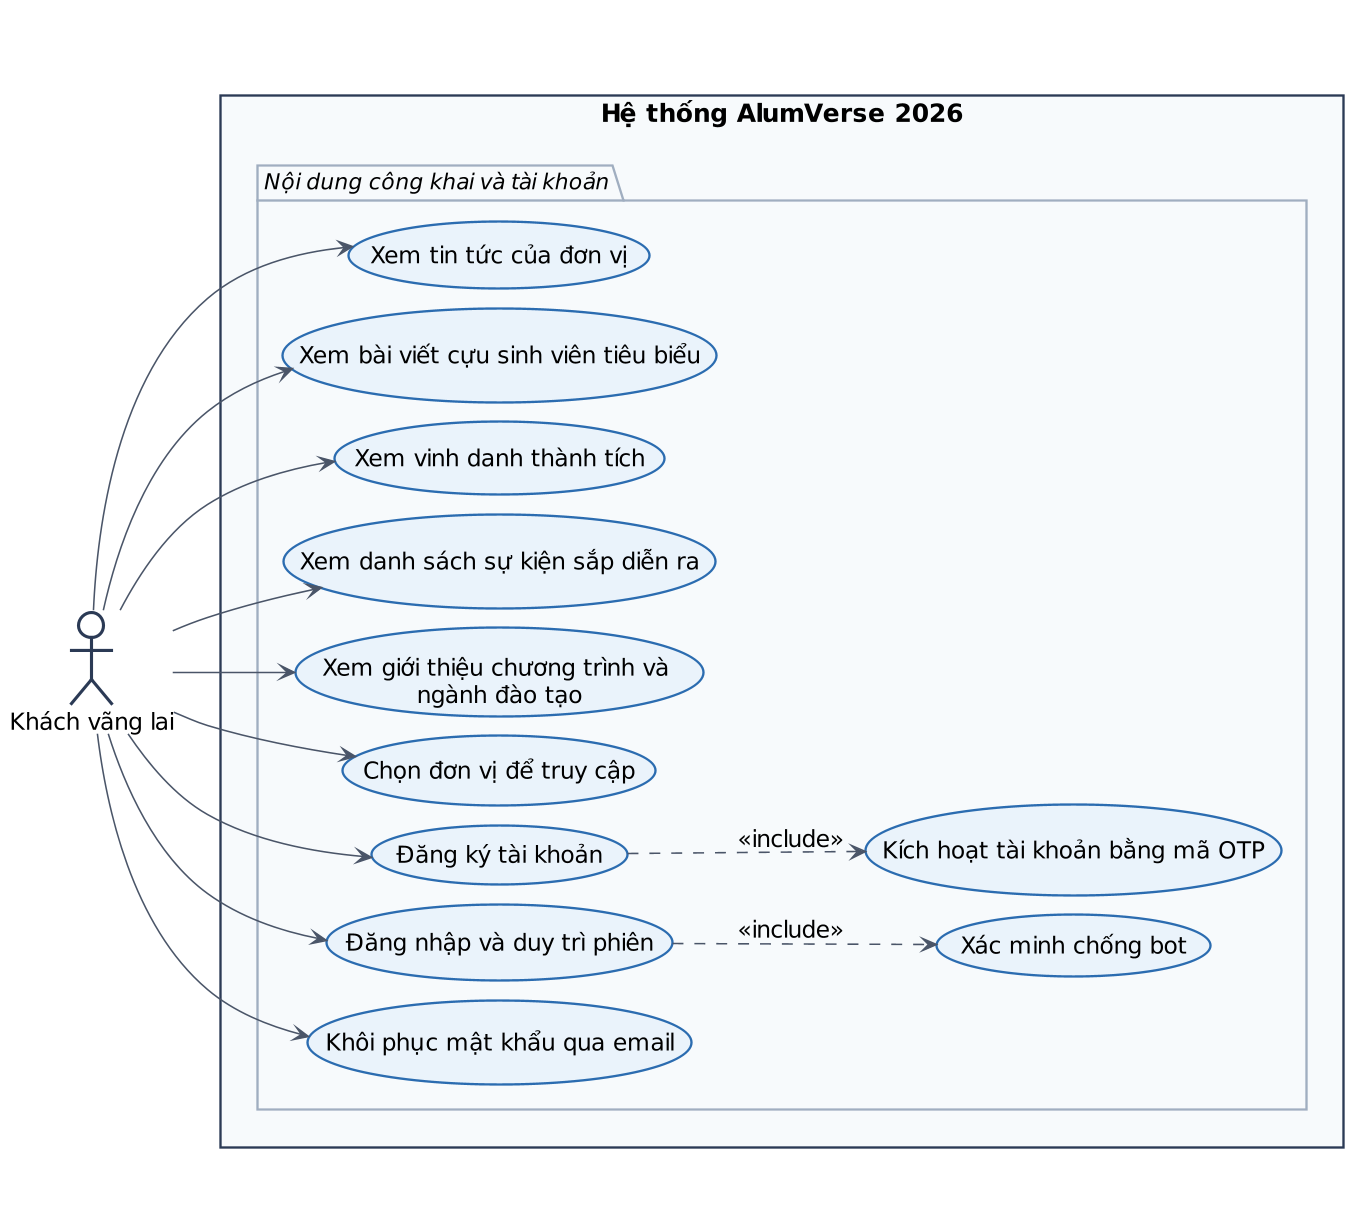
\includegraphics[width=\textwidth,height=0.84\textheight,keepaspectratio]{uc1-guest}
\caption{Sơ đồ use case của tác nhân Khách vãng lai}
\label{fig:ucguest}
\end{figure}

\begin{figure}[H]\centering
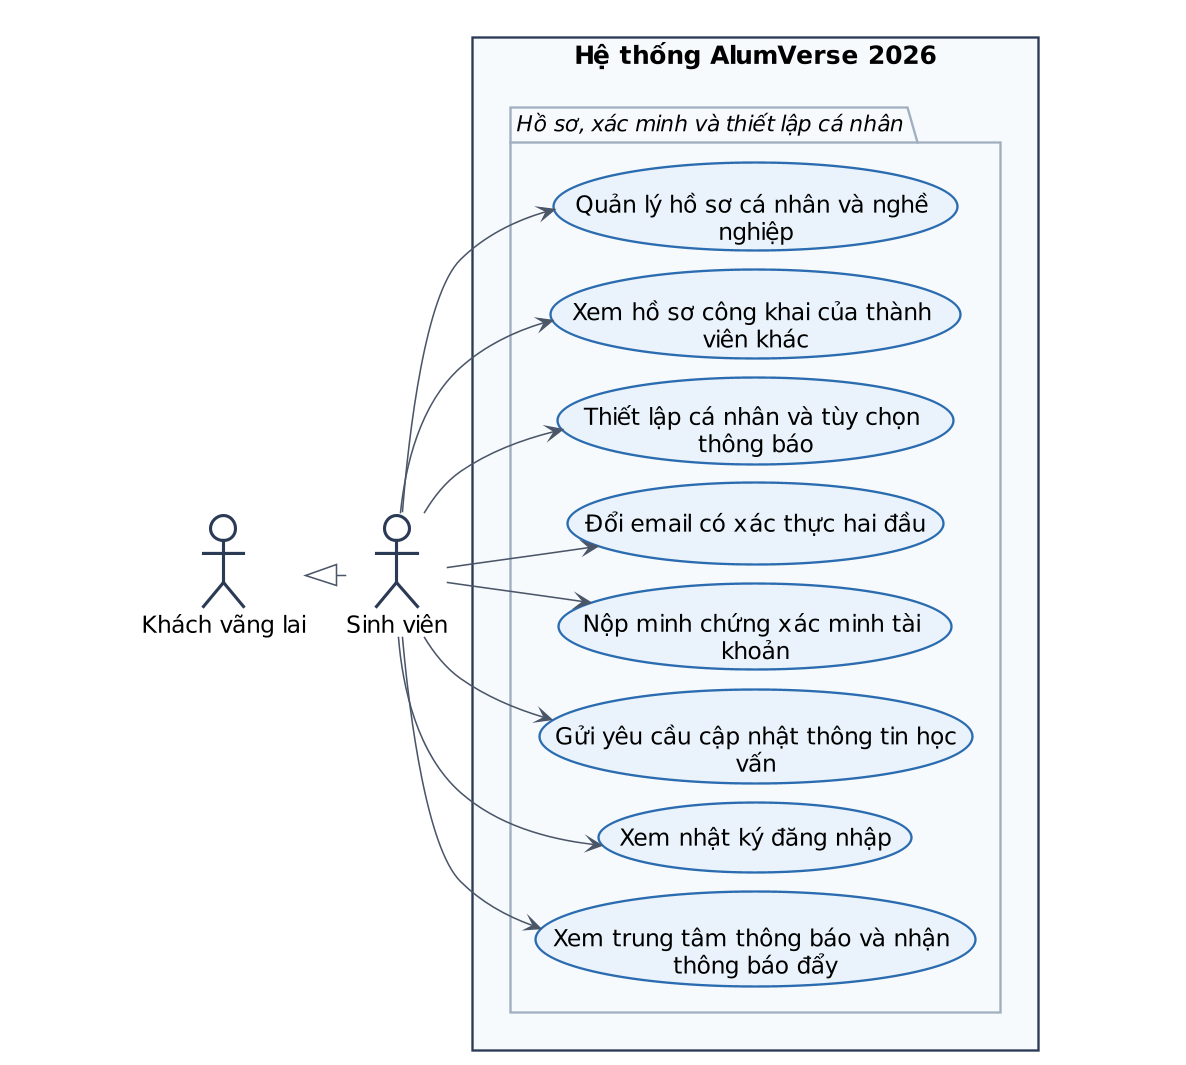
\includegraphics[width=\textwidth,height=0.84\textheight,keepaspectratio]{uc2a-student}
\caption{Sơ đồ use case của tác nhân Sinh viên: hồ sơ, xác minh và thiết lập cá nhân}
\label{fig:ucstudent}
\end{figure}

\begin{figure}[H]\centering
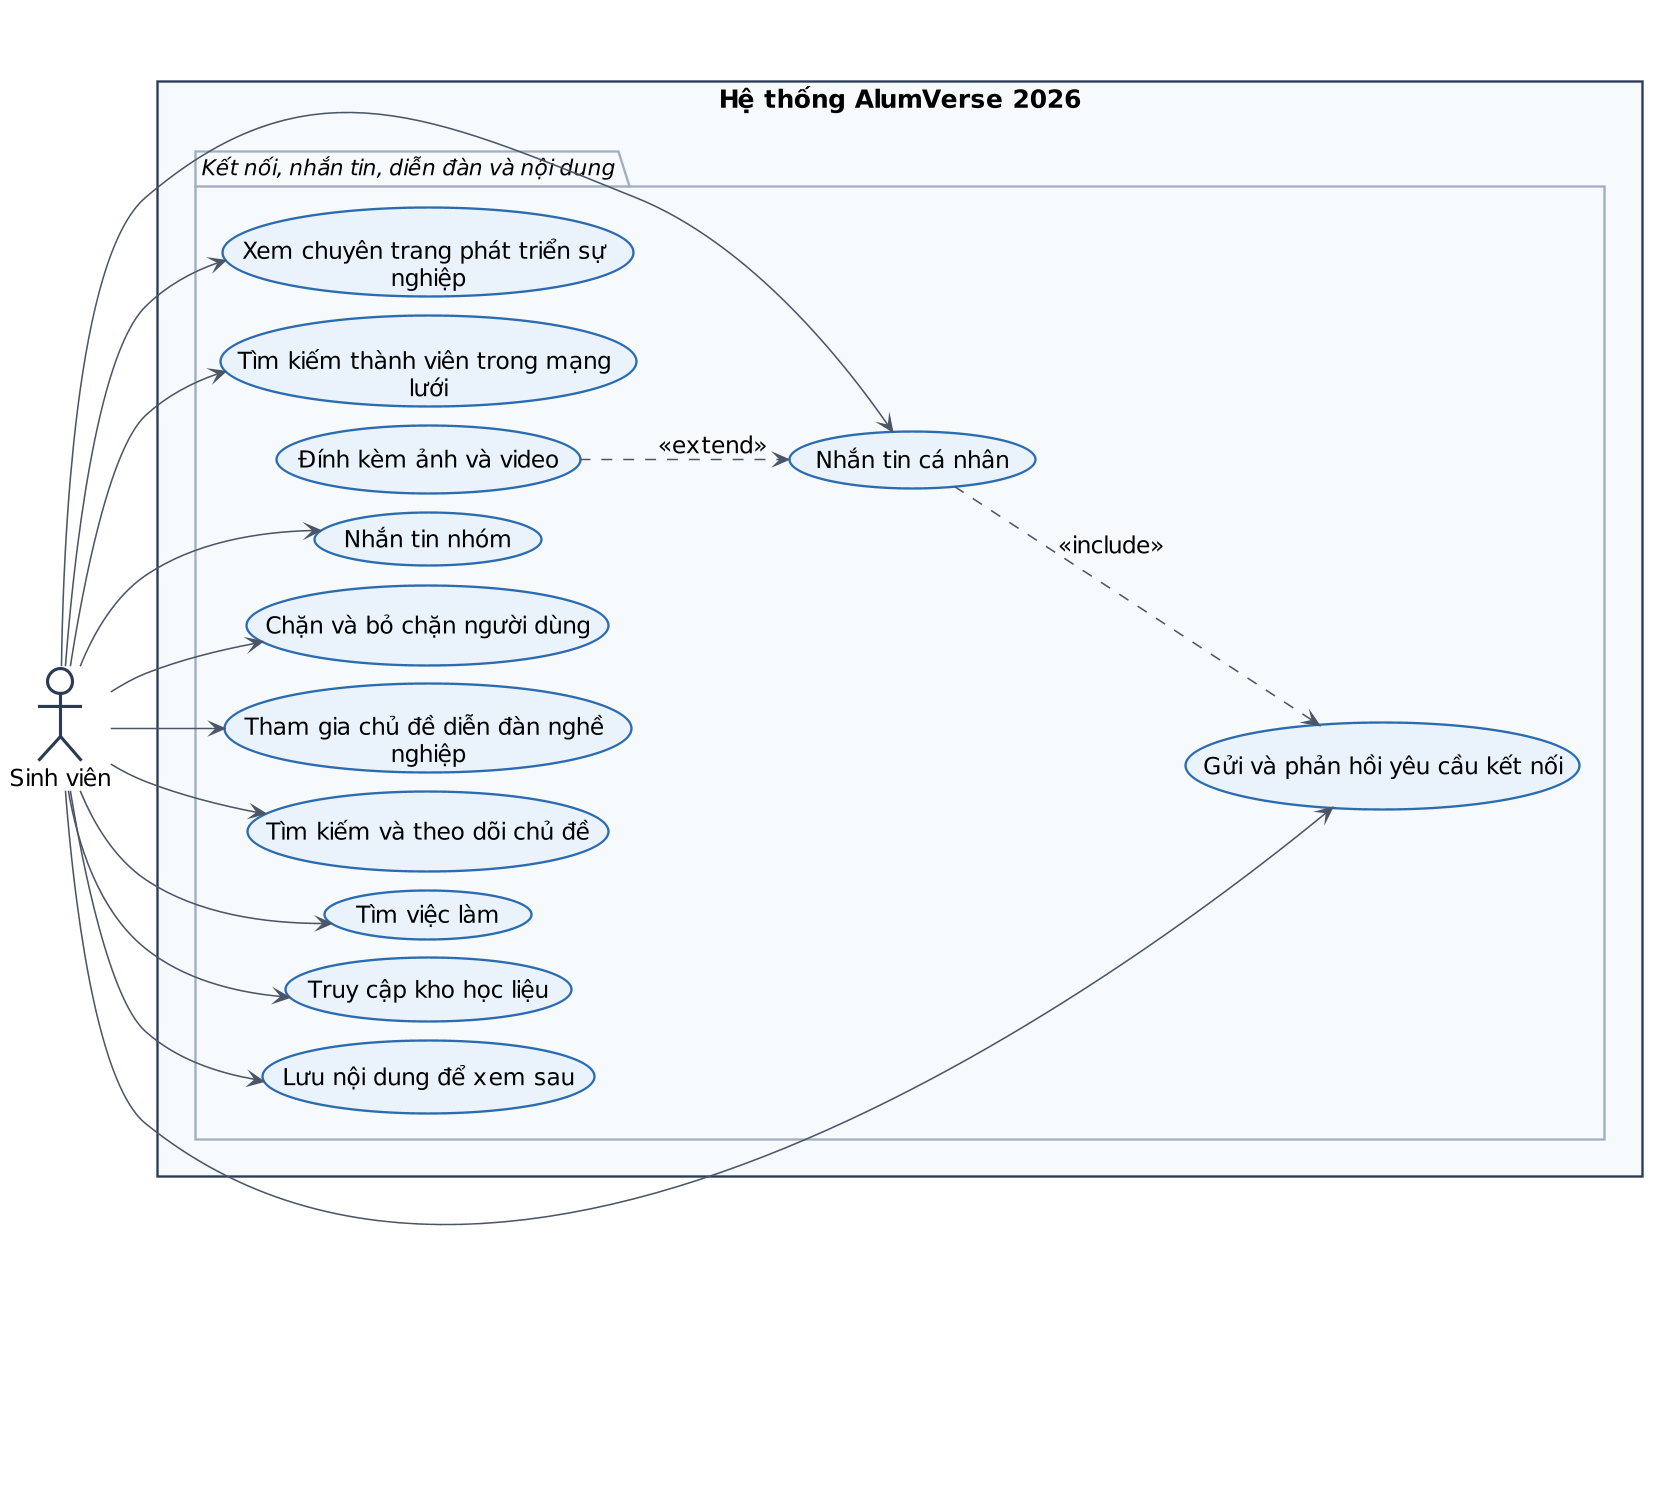
\includegraphics[width=\textwidth,height=0.84\textheight,keepaspectratio]{uc2b-student}
\caption{Sơ đồ use case của tác nhân Sinh viên: kết nối, nhắn tin, diễn đàn và nội dung}
\label{fig:ucstudent2}
\end{figure}

\begin{figure}[H]\centering
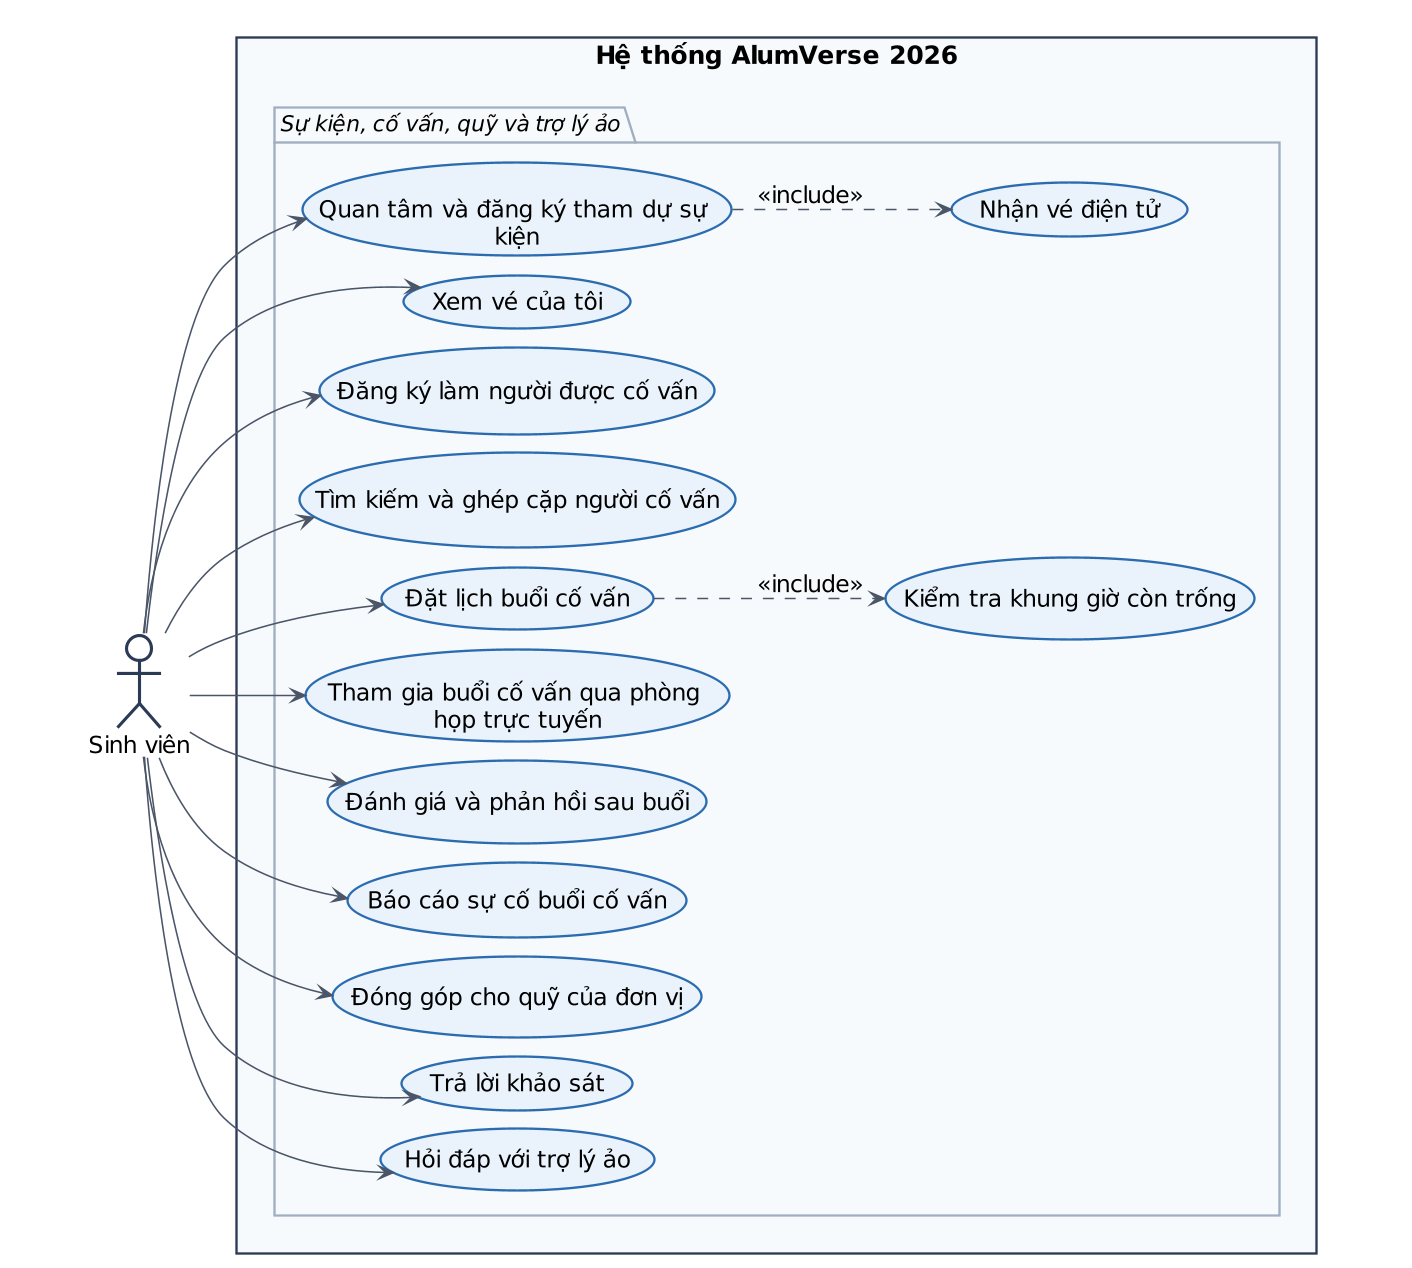
\includegraphics[width=\textwidth,height=0.84\textheight,keepaspectratio]{uc2c-student}
\caption{Sơ đồ use case của tác nhân Sinh viên: sự kiện, cố vấn, quỹ và trợ lý ảo}
\label{fig:ucstudent3}
\end{figure}

\begin{figure}[H]\centering
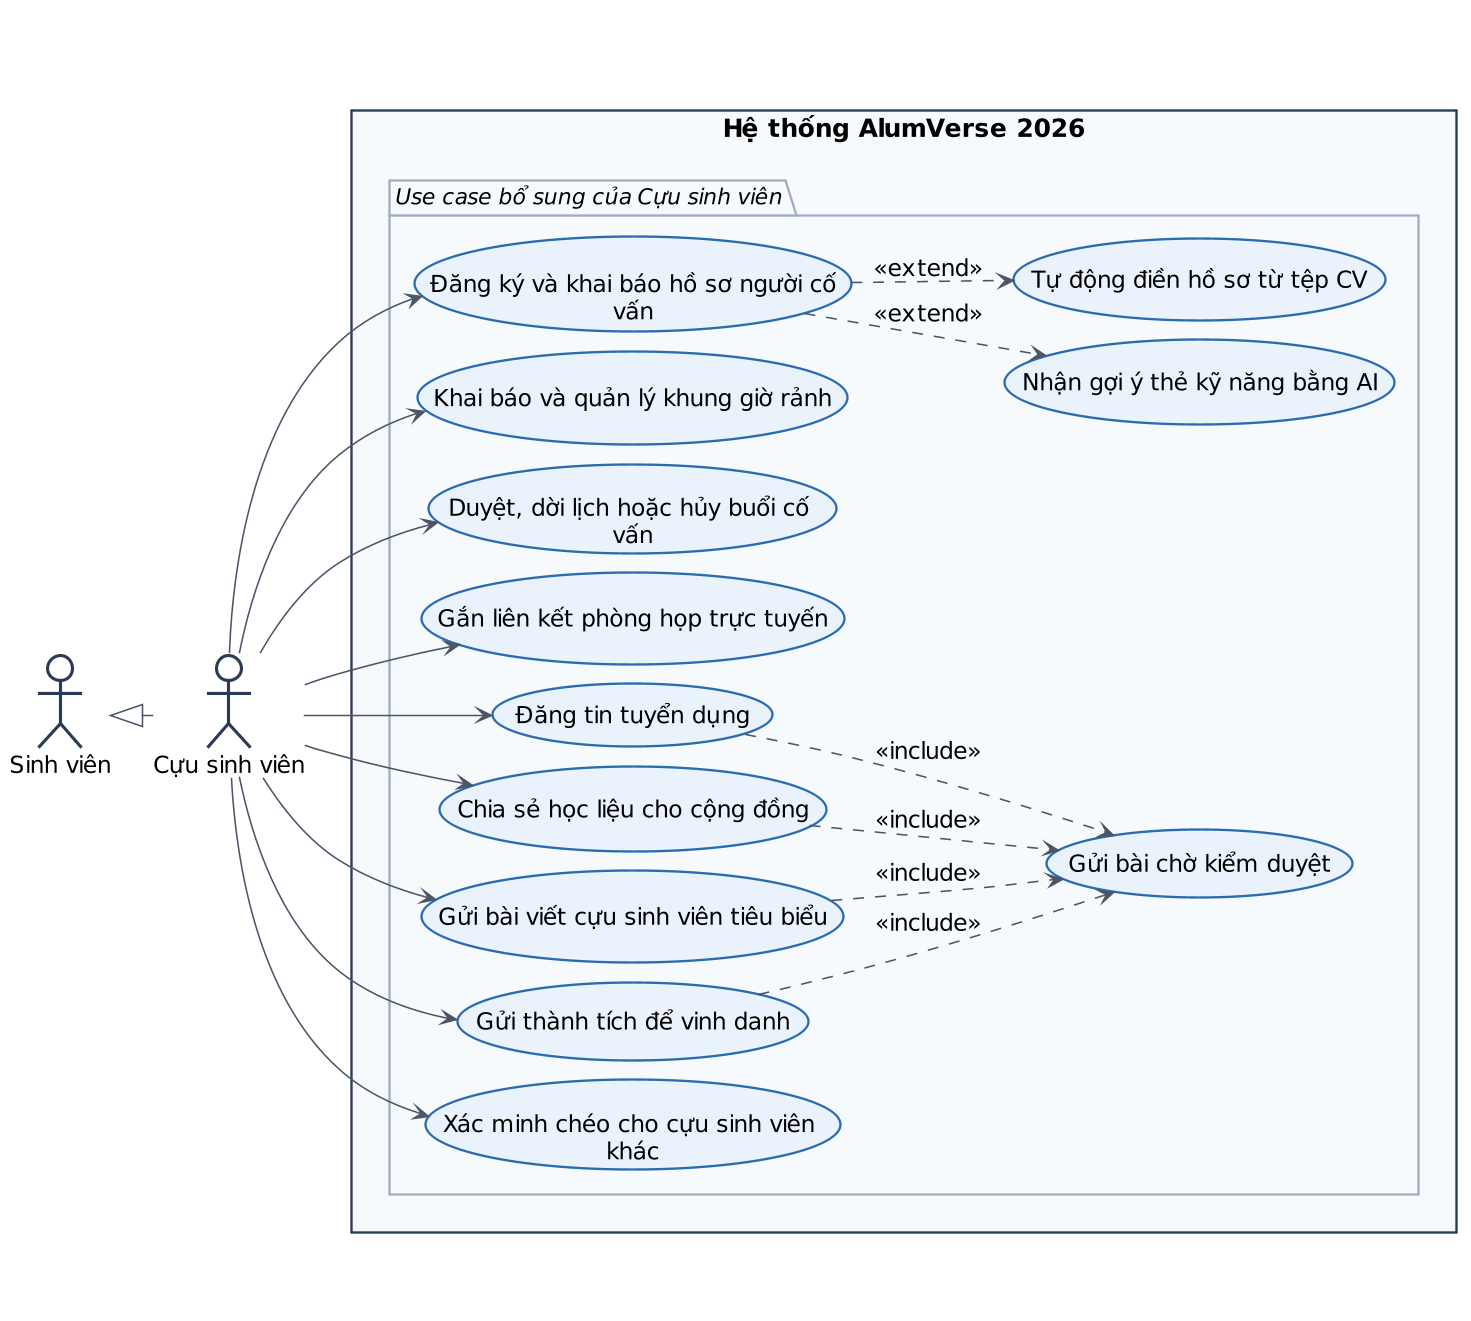
\includegraphics[width=\textwidth,height=0.84\textheight,keepaspectratio]{uc3-alumni}
\caption{Sơ đồ use case bổ sung của tác nhân Cựu sinh viên}
\label{fig:ucalumni}
\end{figure}

\begin{figure}[H]\centering
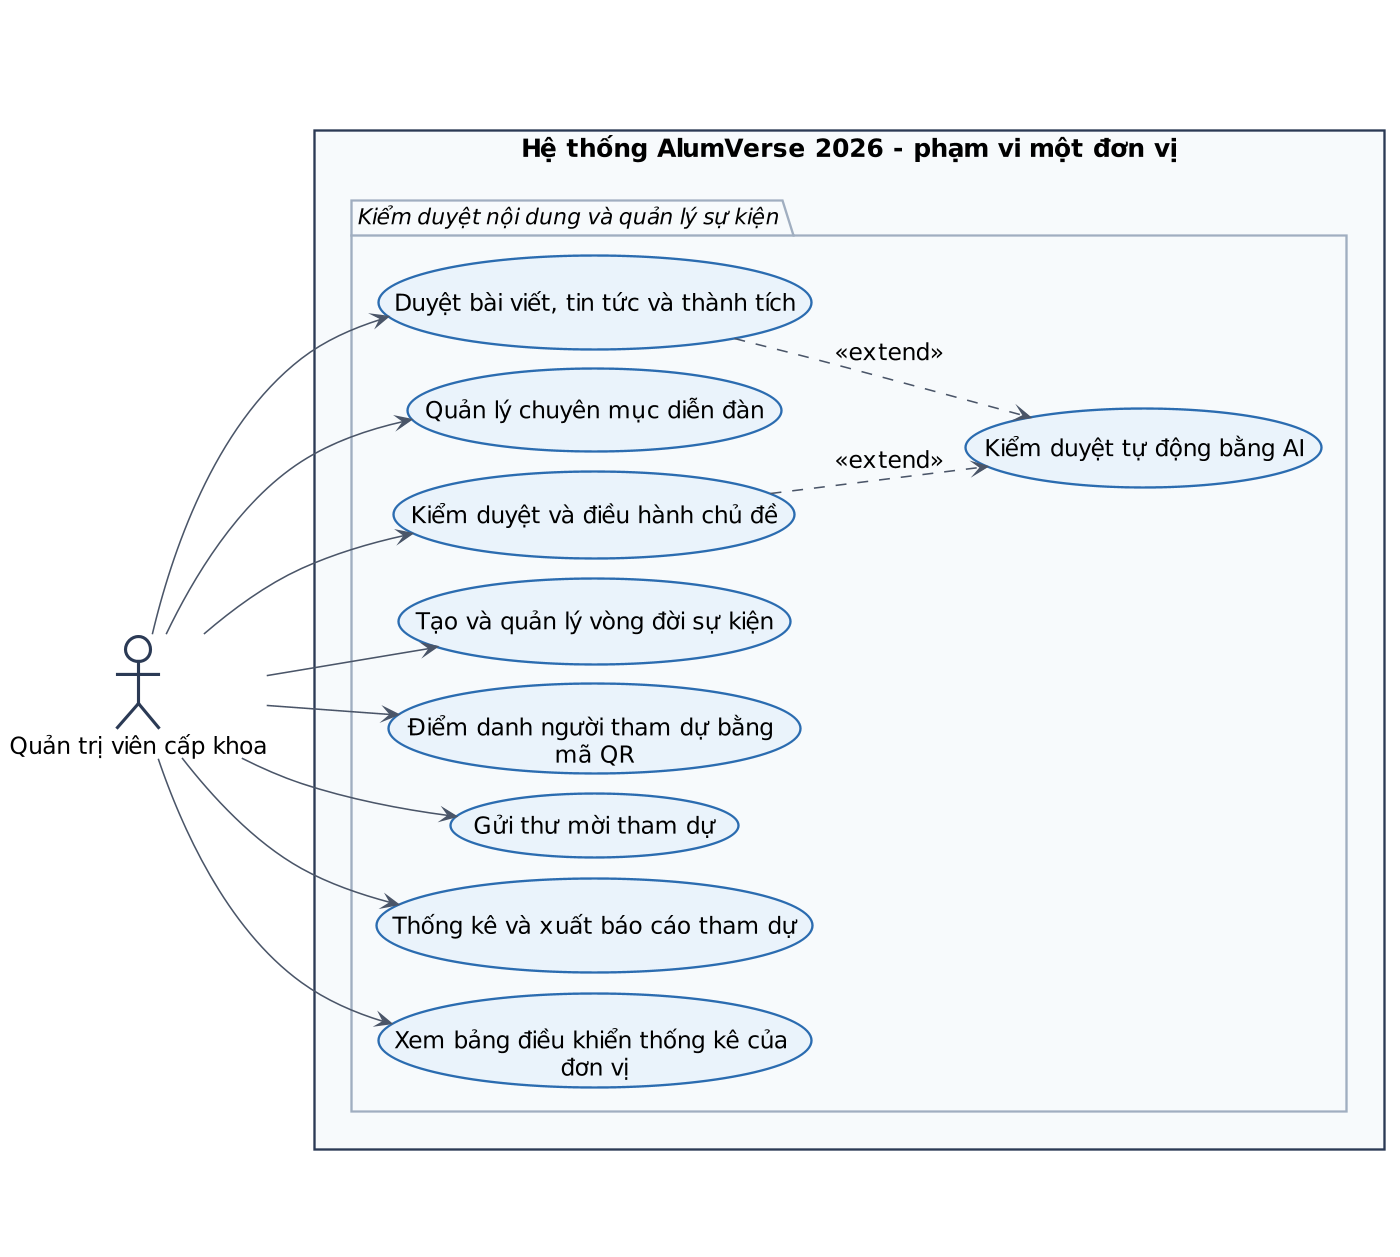
\includegraphics[width=\textwidth,height=0.84\textheight,keepaspectratio]{uc4a-facultyadmin}
\caption{Sơ đồ use case của tác nhân Quản trị viên cấp khoa: kiểm duyệt nội dung và quản lý sự kiện}
\label{fig:ucfadmin}
\end{figure}

\begin{figure}[H]\centering
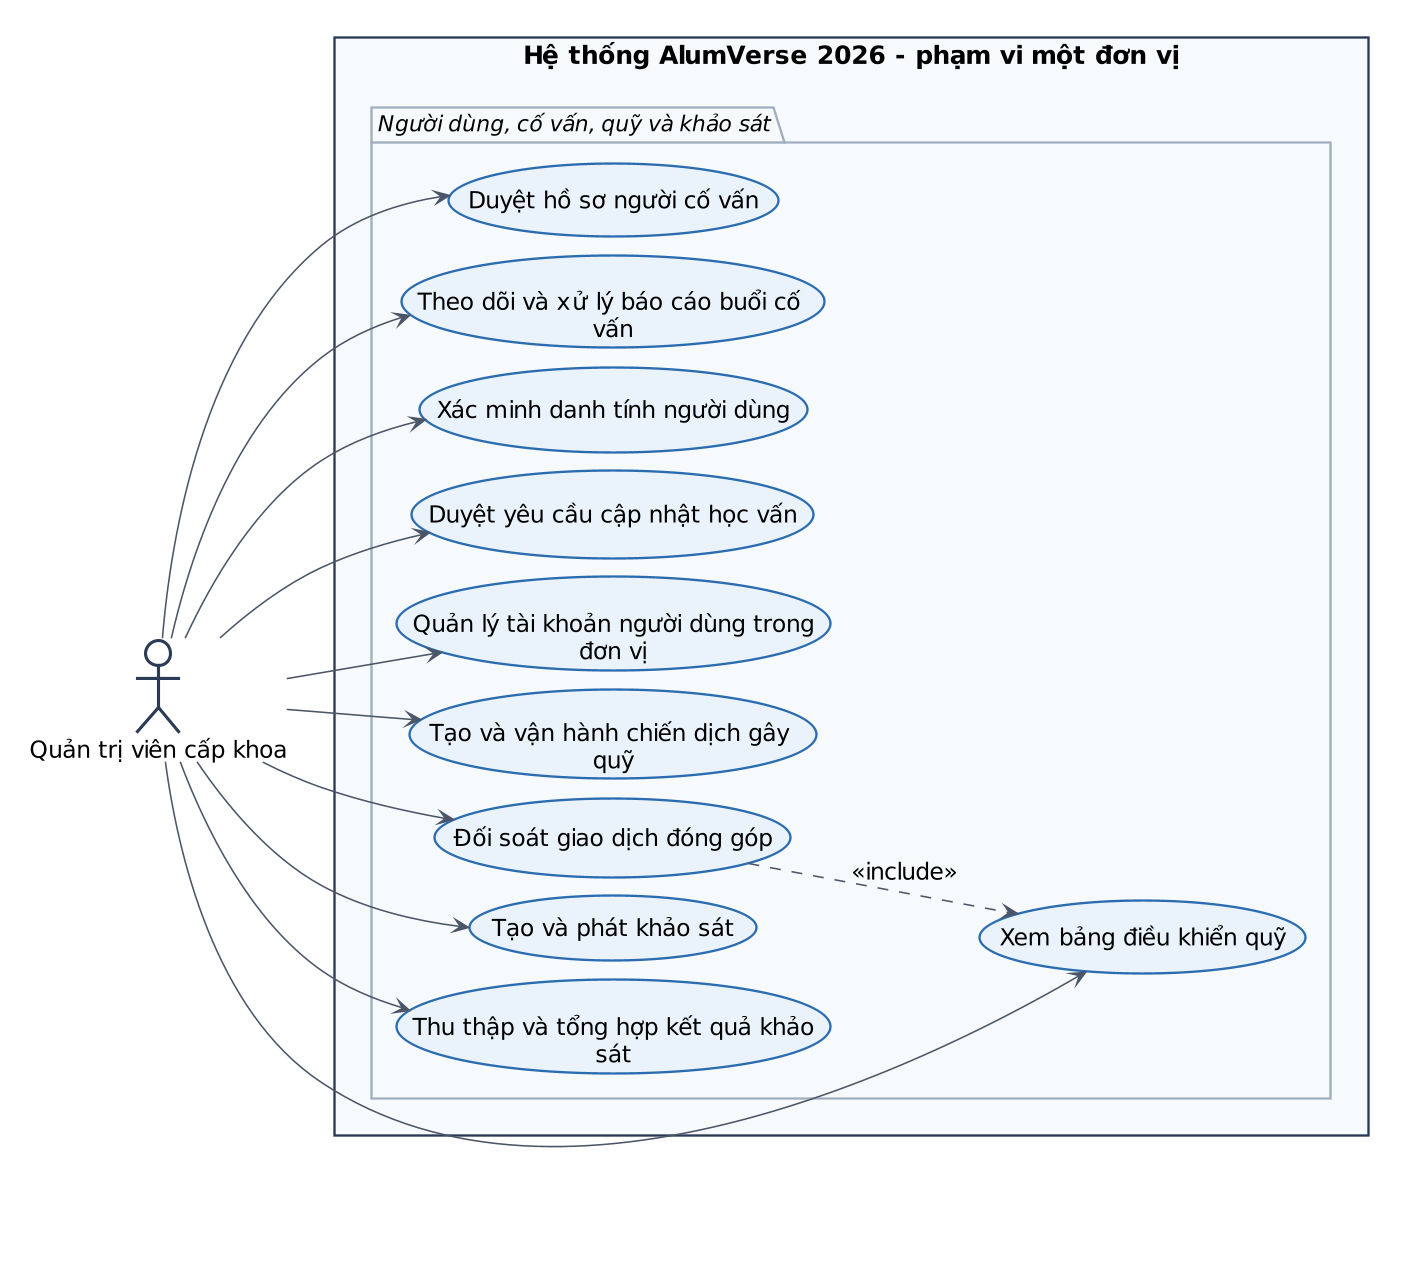
\includegraphics[width=\textwidth,height=0.84\textheight,keepaspectratio]{uc4b-facultyadmin}
\caption{Sơ đồ use case của tác nhân Quản trị viên cấp khoa: người dùng, cố vấn, quỹ và khảo sát}
\label{fig:ucfadmin2}
\end{figure}

\begin{figure}[H]\centering
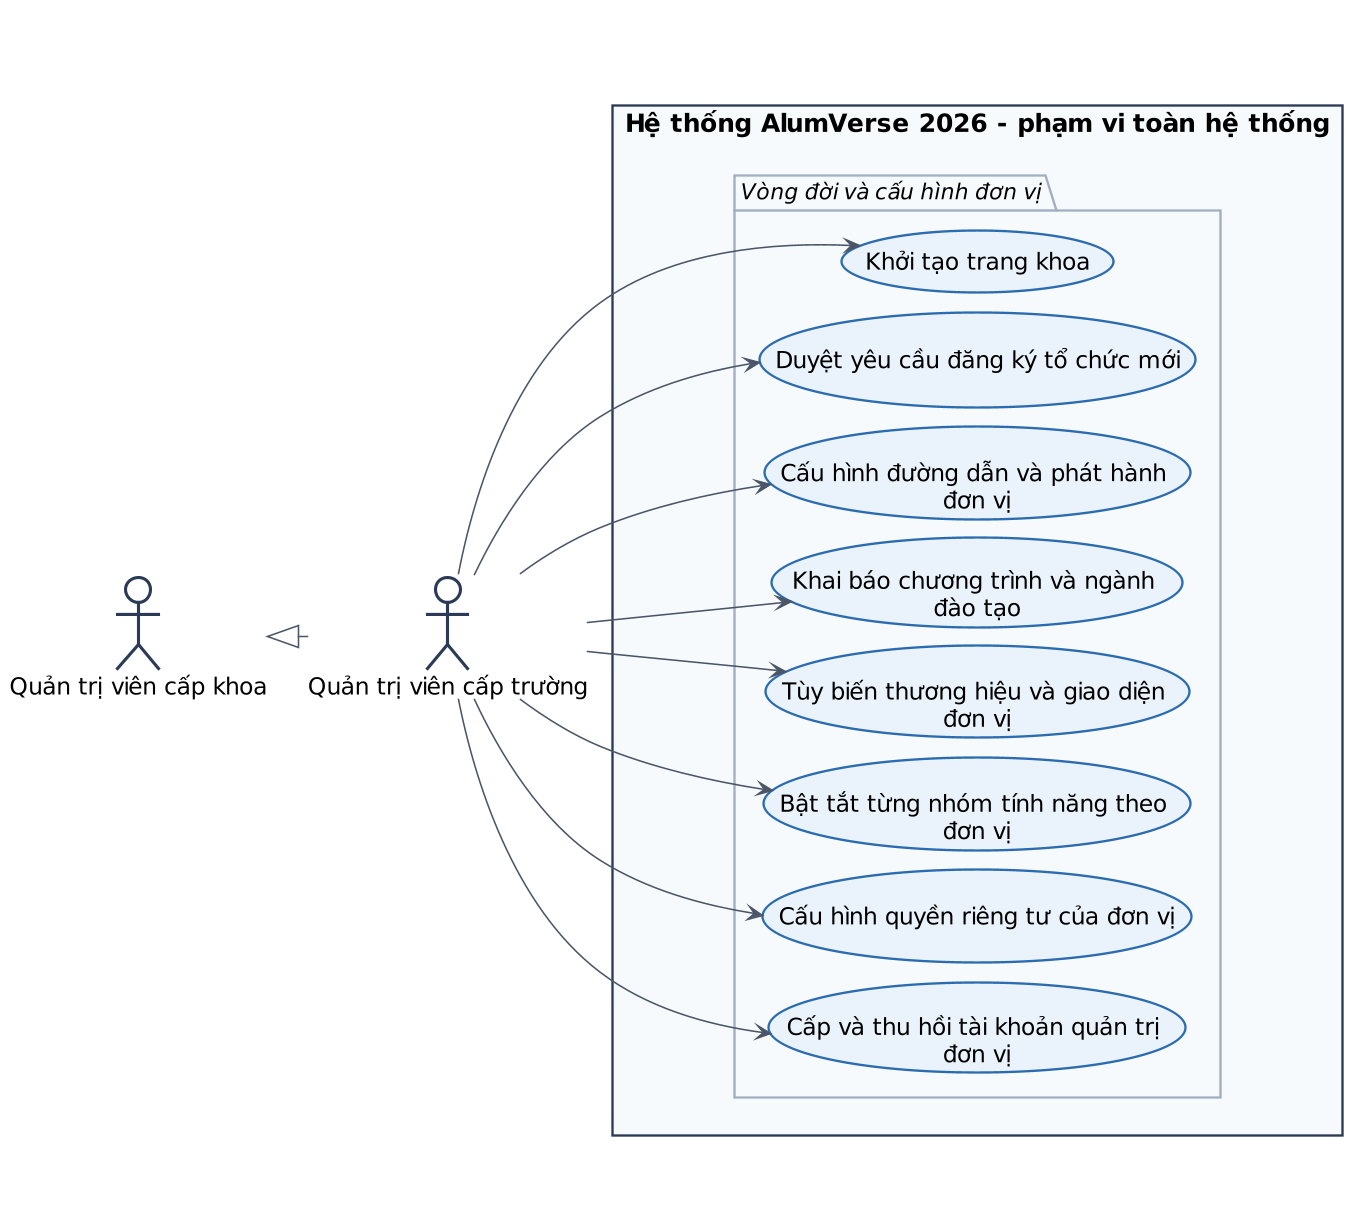
\includegraphics[width=\textwidth,height=0.84\textheight,keepaspectratio]{uc5a-schooladmin}
\caption{Sơ đồ use case bổ sung của tác nhân Quản trị viên cấp trường: vòng đời và cấu hình đơn vị}
\label{fig:ucsadmin}
\end{figure}

\begin{figure}[H]\centering
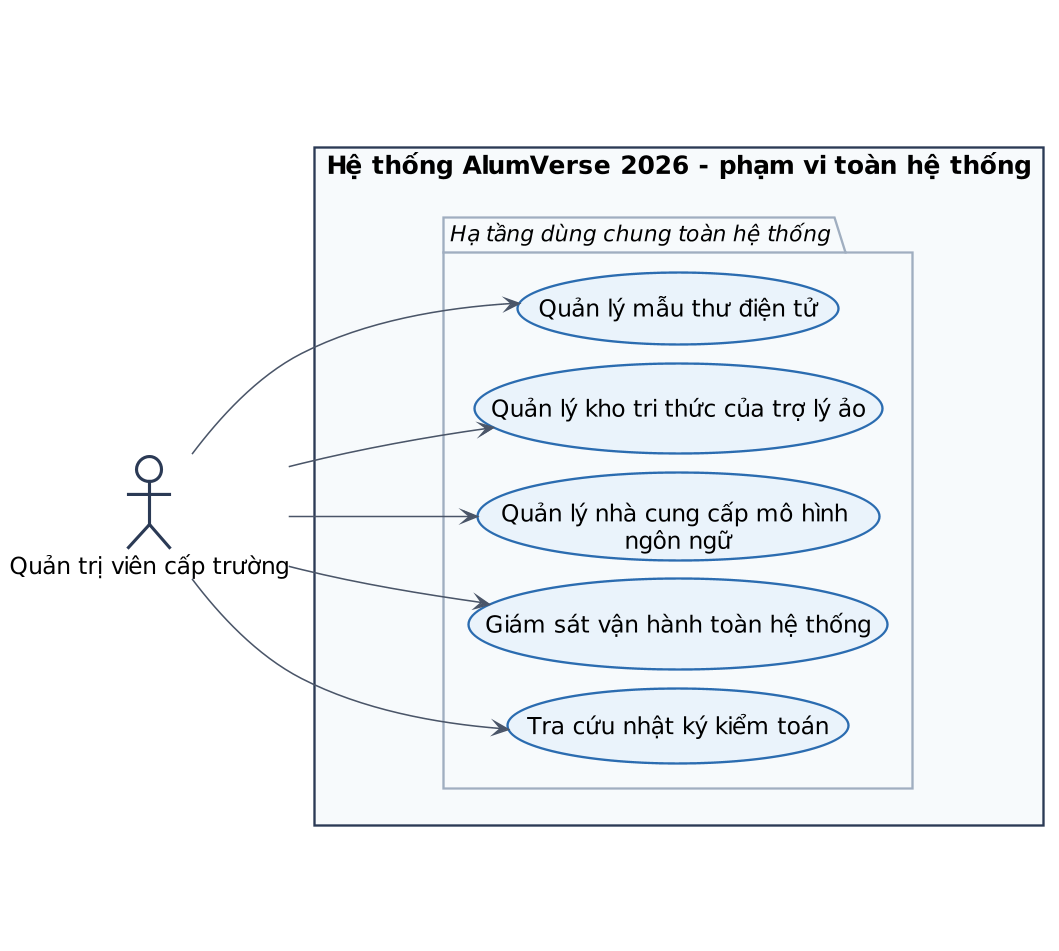
\includegraphics[width=\textwidth,height=0.84\textheight,keepaspectratio]{uc5b-schooladmin}
\caption{Sơ đồ use case bổ sung của tác nhân Quản trị viên cấp trường: hạ tầng dùng chung}
\label{fig:ucsadmin2}
\end{figure}

\subsection{Yêu cầu chức năng}

Danh mục tính năng của hệ thống gồm 86 tính năng thuộc 15 module, là kết quả của quá trình rà soát và hợp nhất từ danh sách theo dõi ban đầu. Quá trình rà soát loại bỏ những mục vốn chỉ là ràng buộc kiểm tra dữ liệu hoặc chi tiết hiện thực, đồng thời gộp các mục nhỏ vào tính năng cha để mỗi dòng trong danh mục thực sự tương ứng với một năng lực mà người dùng cảm nhận được.

Danh mục này là căn cứ thống nhất cho ba việc: phân tích yêu cầu ở chương này, phân công công việc trong nhóm, và đánh giá mức độ hoàn thành ở Chương 5. Danh sách đầy đủ kèm mô tả của từng tính năng được trình bày ở Phụ lục A.

\renewcommand{\arraystretch}{1.25}
{\small
\begin{longtable}{|c|>{\raggedright\arraybackslash}p{7.6cm}|c|c|}
\caption{Các module chức năng và số lượng tính năng}\label{tab:modules}\\
\hline \textbf{STT} & \textbf{Module} & \textbf{Nguồn gốc} & \textbf{Số tính năng} \\ \hline
\endfirsthead
\multicolumn{4}{l}{\itshape\small (tiếp theo trang trước)}\\[2pt]
\hline \textbf{STT} & \textbf{Module} & \textbf{Nguồn gốc} & \textbf{Số tính năng} \\ \hline
\endhead
\hline \multicolumn{4}{r}{\itshape\small (còn tiếp)}\\
\endfoot
\hline
\endlastfoot
1 & Xác thực và phân quyền & Kế thừa 2024 & 12 \\ \hline
2 & Hồ sơ người dùng & Kế thừa 2024 & 3 \\ \hline
3 & Nội dung: tin tức, việc làm, học liệu, vinh danh & Kế thừa 2024 & 8 \\ \hline
4 & Sự kiện & Kế thừa 2024 & 7 \\ \hline
5 & Nhắn tin và mạng lưới kết nối & Kế thừa 2024 & 8 \\ \hline
6 & Diễn đàn & Kế thừa 2024 & 7 \\ \hline
7 & Thông báo & Kế thừa 2024 & 3 \\ \hline
8 & Giao diện và trang công khai & Kế thừa 2024 & 4 \\ \hline
9 & Tổ chức và đa đơn vị & Mới 2026 & 8 \\ \hline
10 & Cố vấn & Mới 2026 & 10 \\ \hline
11 & Gây quỹ & Mới 2026 & 5 \\ \hline
12 & Khảo sát & Mới 2026 & 2 \\ \hline
13 & Trợ lý ảo và ứng dụng AI & Mới 2026 & 4 \\ \hline
14 & Nền tảng dùng chung & Mới 2026 & 3 \\ \hline
15 & Ứng dụng di động & Mới 2026 & 2 \\ \hline
\multicolumn{3}{|r|}{\textbf{Tổng cộng}} & \textbf{86} \\ \hline
\end{longtable}
}
\renewcommand{\arraystretch}{1}

\subsection{Đặc tả use case tiêu biểu}

Hệ thống đặc tả sâu các luồng use case mang tính trọng tâm, là những luồng vừa có giá trị nghiệp vụ cao vừa chứa ràng buộc kỹ thuật phức tạp.

Luồng đăng ký tài khoản kèm kích hoạt bằng mã dùng một lần bảo đảm mỗi tài khoản gắn với một địa chỉ thư điện tử có thật. Luồng khởi tạo hồ sơ người cố vấn được thiết kế theo biểu mẫu nhiều bước có lưu nháp, kèm bước gọi mô hình ngôn ngữ để gợi ý thẻ kỹ năng từ phần mô tả chuyên môn, nhằm giảm rào cản cho người cố vấn như phân tích ở Chương 2. Luồng đặt lịch cố vấn và đánh giá phản hồi chứa ràng buộc chống trùng lịch khi nhiều người cùng đặt một khung giờ. Luồng đóng góp quỹ qua mã QR đi kèm cơ chế đối soát tự động bảo đảm không cộng trùng tiền khi cổng thanh toán gửi lại thông báo nhiều lần. Luồng nhắn tin riêng bắt buộc phải thông qua bước chấp nhận yêu cầu kết nối nhằm chống tin nhắn rác.

\renewcommand{\arraystretch}{1.2}
\begin{longtable}{|>{\raggedright\arraybackslash}p{3.0cm}|>{\raggedright\arraybackslash}p{2.4cm}|>{\raggedright\arraybackslash}p{4.4cm}|>{\raggedright\arraybackslash}p{4.6cm}|}
\caption{Đặc tả một số use case tiêu biểu}\label{tab:usecasespec}\\
\hline \textbf{Use case} & \textbf{Tác nhân} & \textbf{Luồng chính} & \textbf{Ràng buộc và ngoại lệ} \\ \hline
\endfirsthead
\hline \textbf{Use case} & \textbf{Tác nhân} & \textbf{Luồng chính} & \textbf{Ràng buộc và ngoại lệ} \\ \hline
\endhead
Đăng ký và kích hoạt & Khách vãng lai & Nhập thông tin, nhận mã một lần qua thư điện tử, nhập mã để kích hoạt & Mã có thời hạn; nhập sai quá số lần phải yêu cầu lại \\ \hline
Khởi tạo hồ sơ người cố vấn & Cựu sinh viên & Điền biểu mẫu nhiều bước có lưu nháp, hệ thống gợi ý thẻ kỹ năng, gửi duyệt & Chỉ tài khoản đã xác minh; quản trị có thể yêu cầu bổ sung \\ \hline
Đặt lịch cố vấn & Sinh viên & Chọn người cố vấn, chọn khung giờ còn trống, gửi yêu cầu & Từ chối nếu khung giờ đã được đặt trong lúc thao tác \\ \hline
Đóng góp quỹ & Sinh viên, Cựu sinh viên & Chọn chiến dịch, nhận mã QR có định danh riêng, chuyển khoản & Thông báo lặp từ cổng thanh toán bị bỏ qua, không cộng trùng \\ \hline
Nhắn tin riêng & Sinh viên, Cựu sinh viên & Gửi yêu cầu kết nối kèm tin nhắn đầu, chờ chấp nhận, mở hội thoại & Không thể nhắn nếu chưa được chấp nhận hoặc đã bị chặn \\ \hline
\end{longtable}
\renewcommand{\arraystretch}{1}

\subsection{Yêu cầu phi chức năng}

Hệ thống hướng tới bốn nhóm yêu cầu phi chức năng chính.

Về hiệu năng, toàn bộ chuỗi xử lý phải vận hành theo cơ chế bất đồng bộ, không chặn luồng, nhằm phục vụ nhiều kết nối đồng thời với lượng tài nguyên tối thiểu, đặc biệt với các tính năng duy trì kết nối lâu dài như nhắn tin thời gian thực và trợ lý ảo.

Về khả năng phục vụ nhiều đơn vị, hệ thống phải hỗ trợ nhiều khoa trên cùng một lần triển khai, với dữ liệu được cô lập chặt chẽ và không có khả năng rò rỉ chéo giữa các đơn vị.

Về bảo mật, hệ thống phải bảo đảm xác thực bằng token có thời hạn, phân quyền theo vai trò và phạm vi tổ chức, chống truy cập tự động bằng công cụ kiểm tra người dùng thật, chống chèn mã vào câu truy vấn và giới hạn tần suất truy cập với các điểm cuối nhạy cảm.

Về khả năng bảo trì, mã nguồn phải được tổ chức thành các module có ranh giới rõ ràng, mỗi module tuân theo kiến trúc phân lớp thống nhất, kèm kiểm thử tự động cho tầng nghiệp vụ để bảo vệ hành vi hệ thống khi thay đổi.

\section{Kiến trúc nghiệp vụ đa tổ chức}

\subsection{Mô hình đa tổ chức}

Điểm khác biệt lớn nhất về mặt kiến trúc nghiệp vụ giữa phiên bản 2026 và phiên bản 2024 là hệ thống được thiết kế để phục vụ nhiều đơn vị trên cùng một lần triển khai, thay vì mỗi khoa phải vận hành một ứng dụng riêng.

Mỗi tổ chức trong hệ thống là một thực thể độc lập có cấu hình riêng, bao gồm tên và đường dẫn định danh, logo và bộ nhận diện thương hiệu, nội dung giới thiệu đơn vị, danh mục ngành và chương trình đào tạo, cấu hình bật tắt từng nhóm tính năng, và danh sách tài khoản quản trị thuộc phạm vi đơn vị đó. Cấu hình bật tắt tính năng cho phép mỗi khoa lựa chọn nhóm tính năng phù hợp với nhu cầu thực tế thay vì buộc phải dùng trọn bộ.

Một người dùng có thể thuộc về nhiều tổ chức, phản ánh thực tế một cựu sinh viên có thể học nhiều chương trình ở các khoa khác nhau. Khi người dùng chuyển đổi tổ chức đang xem, hệ thống cấp lại ngữ cảnh làm việc tương ứng và toàn bộ dữ liệu hiển thị được lọc theo tổ chức mới.

\begin{figure}[H]\centering
\begin{tikzpicture}[font=\footnotesize,
 b/.style={draw,rounded corners=2pt,align=center,inner sep=3pt},
 org/.style={b,fill=green!10,minimum height=9mm,text width=26mm},
 usr/.style={b,fill=blue!8,minimum height=7mm,text width=22mm},
 ar/.style={-{Latex[length=2mm]},thick}]
\node[b,fill=gray!10,minimum height=8mm,text width=44mm] (sys) at (4.4,2.0)
 {Một lần triển khai duy nhất\\ \scriptsize alumverse.hcmus.edu.vn};
\node[org] (o1) at (0,0.2)   {Khoa A\\ \scriptsize /fit};
\node[org] (o2) at (4.4,0.2) {Khoa B\\ \scriptsize /math};
\node[org] (o3) at (8.8,0.2) {Khoa C\\ \scriptsize /chem};
\node[b,fill=yellow!14,text width=48mm,align=left,font=\scriptsize] (cfg) at (4.4,-2.0)
 {Mỗi tổ chức có riêng: logo và bộ nhận diện, nội dung giới thiệu, ngành đào tạo, cấu hình bật tắt tính năng, tài khoản quản trị};
\node[usr] (u) at (0,-4.9) {Người dùng};
\node[b,fill=orange!10,text width=46mm,align=left,font=\scriptsize] (multi) at (6.4,-4.9)
 {Một người dùng có thể thuộc nhiều tổ chức; khi chuyển tổ chức, toàn bộ dữ liệu hiển thị được lọc lại theo tổ chức mới};
\draw[ar] (sys) -- (o1); \draw[ar] (sys) -- (o2); \draw[ar] (sys) -- (o3);
\draw[ar,dashed] (o2) -- (cfg);
\draw[ar] (u) -- (o1.south);
\draw[ar,dashed] (u) -- (multi);
\end{tikzpicture}
\caption{Mô hình đa tổ chức của hệ thống AlumVerse 2026}
\label{fig:multiorg}
\end{figure}

\subsection{Cô lập dữ liệu và phân quyền theo tổ chức}

Cơ chế cô lập dữ liệu là yêu cầu bảo mật quan trọng nhất của mô hình đa đơn vị. Hệ thống áp dụng ba lớp bảo vệ chồng lên nhau.

Lớp thứ nhất nằm ở mô hình dữ liệu. Mọi bảng nghiệp vụ đều mang cột định danh tổ chức, và mọi câu truy vấn đọc hay ghi đều bắt buộc kèm điều kiện lọc theo cột này.

Lớp thứ hai nằm ở tầng xác thực. Khi người dùng đăng nhập, định danh tổ chức được nhúng trực tiếp vào token cùng với định danh người dùng và vai trò. Nhờ đó, phạm vi tổ chức đi kèm mọi yêu cầu mà không cần truyền riêng.

Lớp thứ ba nằm ở tầng nghiệp vụ. Hệ thống luôn lấy định danh tổ chức từ token đã ký thay vì tin tưởng giá trị do phía giao diện gửi lên. Đây là điểm mấu chốt: nếu chấp nhận định danh tổ chức từ phía client, một tài khoản quản trị khoa hoàn toàn có thể sửa tham số để thao tác trên dữ liệu của khoa khác.

Về phân quyền, hệ thống kết hợp vai trò với phạm vi tổ chức. Hai tài khoản cùng mang vai trò quản trị nhưng thuộc hai tổ chức khác nhau sẽ thao tác trên hai tập dữ liệu hoàn toàn tách biệt. Riêng vai trò quản trị cấp trường có phạm vi bao trùm toàn hệ thống.

\begin{figure}[H]\centering
\begin{tikzpicture}[font=\footnotesize,node distance=7mm,
 b/.style={draw,rounded corners=2pt,align=center,inner sep=3pt,minimum height=7mm,text width=34mm},
 ar/.style={-{Latex[length=2mm]},thick}]
\node[b,fill=blue!8] (req) {Yêu cầu từ giao diện\\ \scriptsize kèm token đã ký};
\node[b,fill=yellow!14,below=of req] (jwt) {Token chứa userId, vai trò\\ và \texttt{organization\_id}};
\node[b,fill=green!10,below=of jwt] (ctx) {Trích xuất từ ngữ cảnh\\ bảo mật phản ứng};
\node[b,fill=green!10,below=of ctx] (svc) {Tầng nghiệp vụ};
\node[b,fill=orange!10,below=of svc] (dao) {Truy vấn luôn kèm\\ \texttt{WHERE organization\_id = ?}};
\node[cylinder,shape border rotate=90,draw,fill=gray!12,minimum height=8mm,minimum width=26mm,below=7mm of dao] (db) {PostgreSQL};
\node[b,fill=red!8,right=12mm of jwt,text width=36mm] (bad)
 {\texttt{organization\_id} do client gửi lên\\ \textit{bị bỏ qua hoàn toàn}};
\draw[ar] (req)--(jwt); \draw[ar] (jwt)--(ctx); \draw[ar] (ctx)--(svc);
\draw[ar] (svc)--(dao); \draw[ar] (dao)--(db);
\draw[-{Latex[length=2mm]},thick,red!60,dashed] (bad) -- (jwt);
\node[right=4mm of dao,font=\scriptsize,align=left,text width=30mm]
 {Điều kiện lọc là bắt buộc ở mọi truy vấn đọc và ghi};
\end{tikzpicture}
\caption{Cơ chế lọc dữ liệu theo định danh tổ chức}
\label{fig:orgfilter}
\end{figure}

\subsection{Các phân hệ chức năng chính}

Hệ thống được chia thành mười hai phân hệ nghiệp vụ, mỗi phân hệ có ranh giới trách nhiệm rõ ràng.

Phân hệ xác thực chịu trách nhiệm đăng ký, đăng nhập, kích hoạt, khôi phục mật khẩu và cấp phát token. Phân hệ quản lý người dùng phụ trách hồ sơ cá nhân, học vấn, quá trình công tác và quy trình xác minh danh tính. Phân hệ quản lý tổ chức phụ trách khởi tạo, cấu hình và vận hành từng đơn vị. Phân hệ nội dung quản lý tin tức, bài viết cựu sinh viên tiêu biểu, thành tích, tin tuyển dụng và học liệu. Phân hệ sự kiện phụ trách vòng đời sự kiện từ tạo, đăng ký, phát hành vé đến điểm danh và thống kê. Phân hệ nhắn tin phụ trách hội thoại cá nhân, hội thoại nhóm và truyền tin thời gian thực. Phân hệ diễn đàn quản lý chuyên mục, chủ đề, bài thảo luận và kiểm duyệt. Phân hệ gây quỹ phụ trách chiến dịch, đóng góp và đối soát giao dịch. Phân hệ cố vấn phụ trách hồ sơ người cố vấn, ghép cặp, đặt lịch và đánh giá. Phân hệ khảo sát phụ trách tạo biểu mẫu, thu thập và tổng hợp kết quả. Phân hệ thông báo phụ trách thông báo trong ứng dụng và đẩy thời gian thực. Phân hệ trợ lý ảo phụ trách hỏi đáp dựa trên kho tài liệu của nhà trường.

\section{Thiết kế kiến trúc hệ thống}

\subsection{Kiến trúc tổng thể}

Backend là một ứng dụng Spring Boot duy nhất, được tổ chức theo kiến trúc Modular Monolith với mười ba module nghiệp vụ tương ứng các package: \texttt{auth}, \texttt{user}, \texttt{organization}, \texttt{admin}, \texttt{article}, \texttt{event}, \texttt{forum}, \texttt{fundraising}, \texttt{mentorship}, \texttt{chat}, \texttt{survey}, \texttt{config} và \texttt{shared}.

Cần phân biệt hai cách phân nhóm đang cùng tồn tại trong báo cáo. Mười lăm module ở Bảng \ref{tab:modules} là cách phân nhóm theo góc nhìn nghiệp vụ và tính năng, phục vụ việc theo dõi tiến độ. Mười ba module ở đây là cách tổ chức mã nguồn theo package. Hai cách phân nhóm không trùng khớp một đối một vì một số nhóm tính năng như giao diện công khai hay ứng dụng di động không tương ứng với một package backend riêng.

Mỗi module tuân theo kiến trúc Layered với luồng xử lý thống nhất: yêu cầu đi vào controller, controller kiểm tra dữ liệu đầu vào và gọi service, service xử lý nghiệp vụ và gọi lớp truy cập dữ liệu, lớp này truy xuất PostgreSQL thông qua R2DBC. Việc bắt buộc mọi module tuân theo cùng một cấu trúc tầng giúp một thành viên có thể đọc hiểu module do người khác viết mà không cần làm quen lại từ đầu.

Cách chia module theo nghiệp vụ mang lại hai lợi ích thực tế cho một nhóm sáu người. Thứ nhất, nó giảm đáng kể xung đột khi hợp nhất mã nguồn, vì mỗi thành viên làm việc chủ yếu trong phạm vi package của mình. Thứ hai, nó giữ lại khả năng tách một module thành dịch vụ độc lập về sau nếu quy mô hệ thống thực sự đòi hỏi, mà không phải viết lại từ đầu. Cần nhấn mạnh rằng đây là một tùy chọn được bảo lưu chứ không phải mục tiêu của đề tài, bởi phân tích ở Chương 2 đã chỉ ra kiến trúc phân tán không phù hợp với quy mô hiện tại.

\begin{figure}[H]\centering
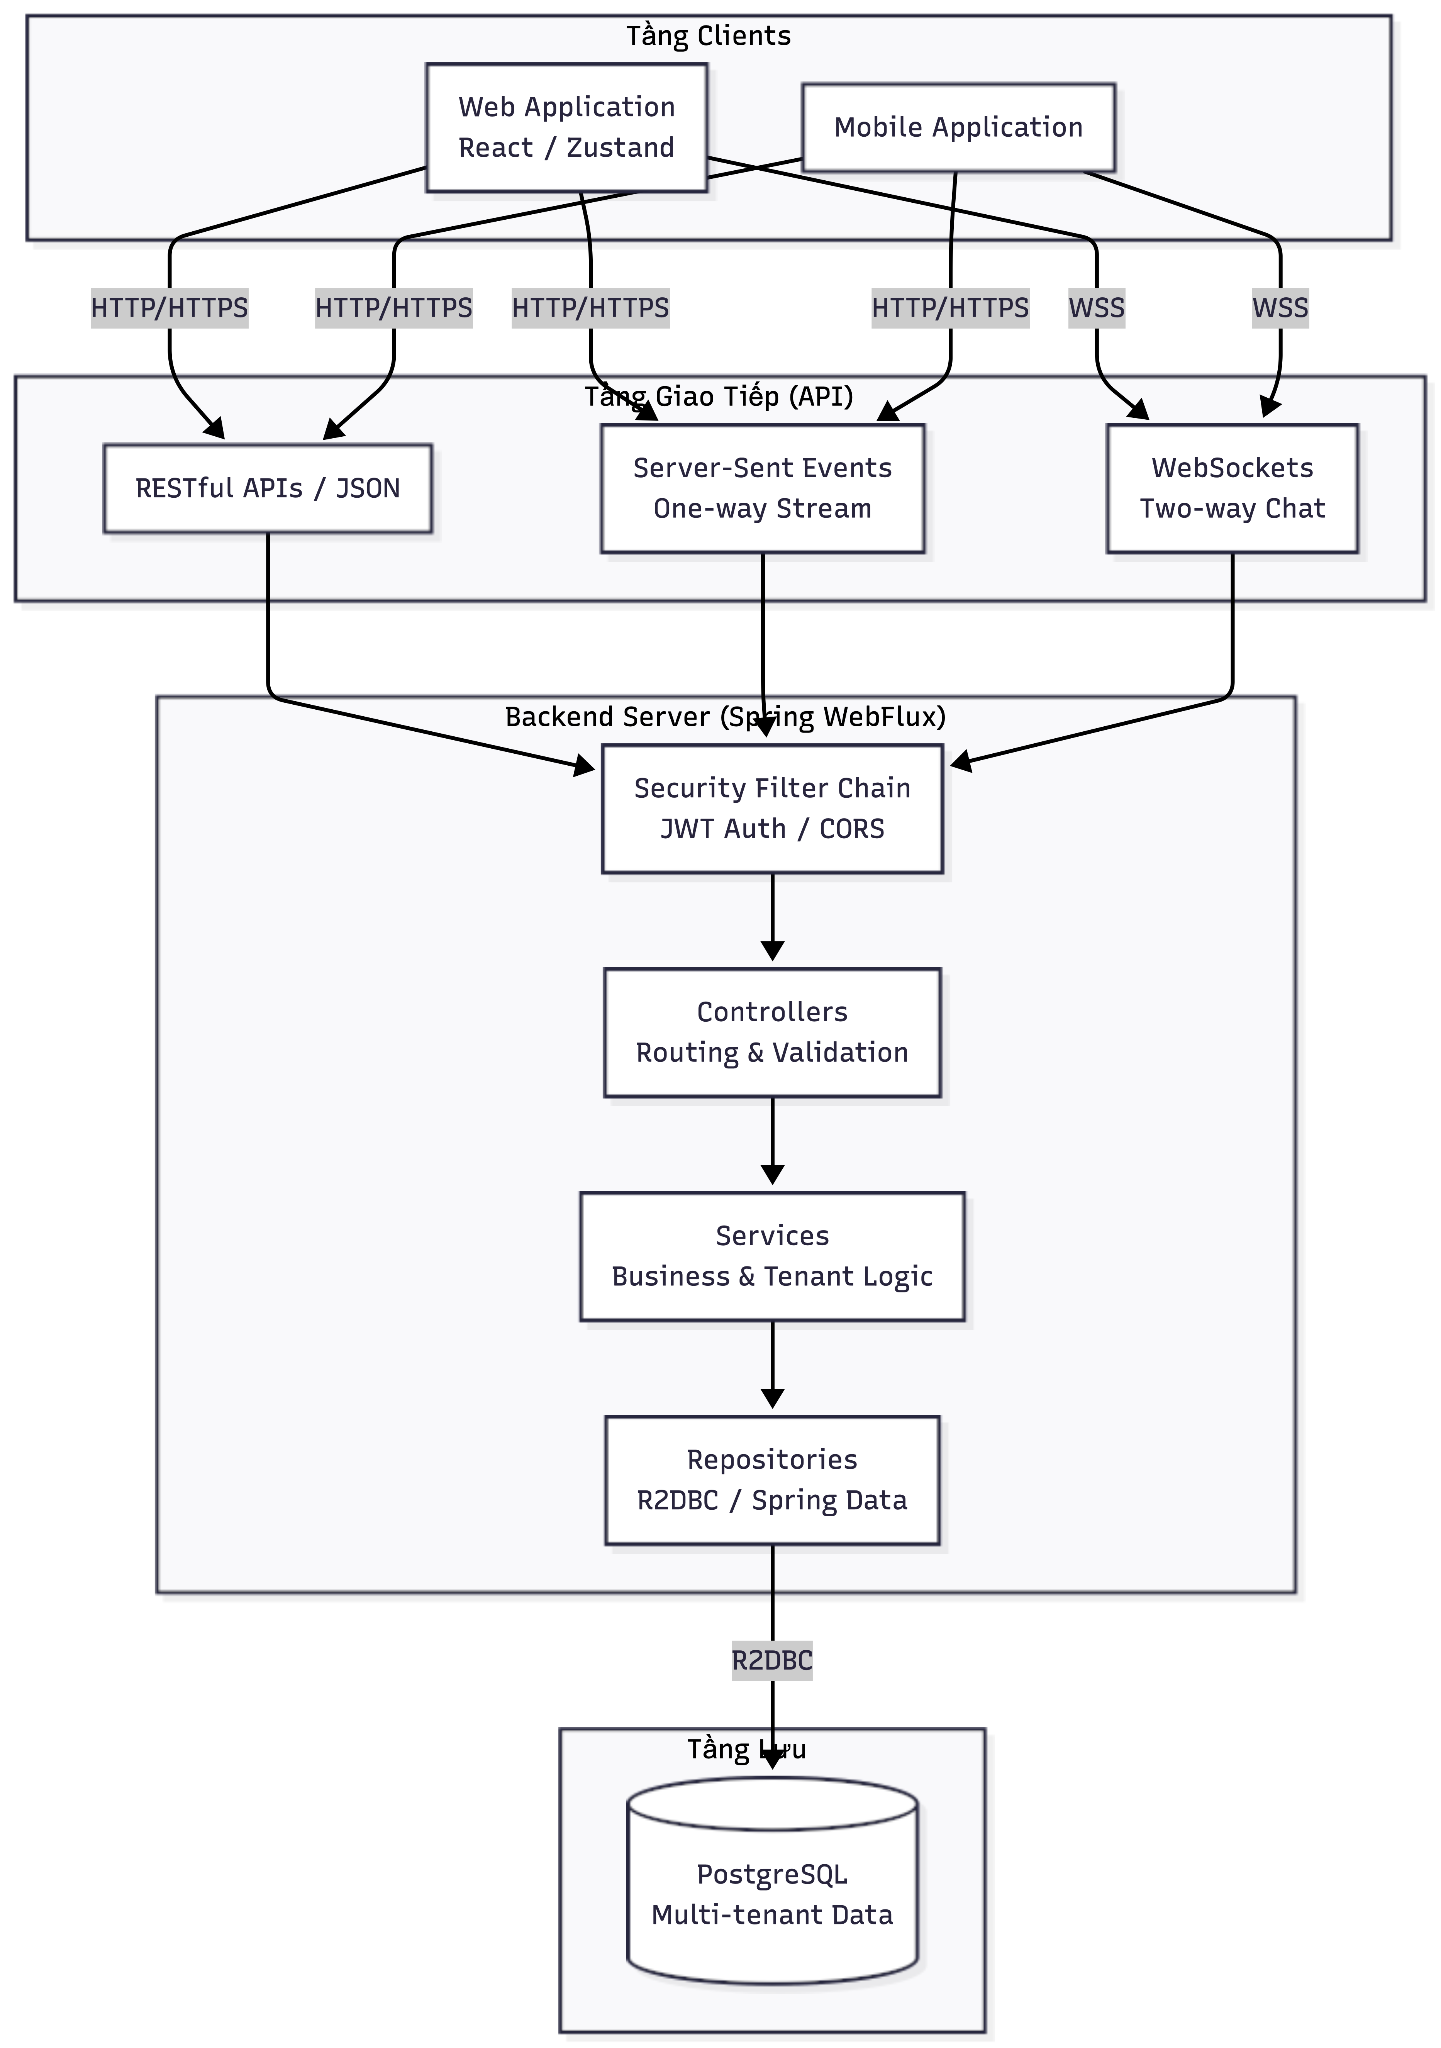
\includegraphics[width=0.78\textwidth,keepaspectratio]{sd-kien-truc-3tang}
\caption{Kiến trúc tổng thể của hệ thống AlumVerse 2026}
\label{fig:arch2026}
\end{figure}

\renewcommand{\arraystretch}{1.2}
\begin{longtable}{|>{\raggedright\arraybackslash}p{3.0cm}|>{\raggedright\arraybackslash}p{11.5cm}|}
\caption{Các module mã nguồn và trách nhiệm}\label{tab:packages}\\
\hline \textbf{Module} & \textbf{Trách nhiệm} \\ \hline
\endfirsthead
\hline \textbf{Module} & \textbf{Trách nhiệm} \\ \hline
\endhead
\texttt{auth} & Đăng ký, đăng nhập, kích hoạt, khôi phục mật khẩu, cấp và thu hồi token \\ \hline
\texttt{user} & Hồ sơ cá nhân, học vấn, quá trình công tác, xác minh danh tính \\ \hline
\texttt{organization} & Khởi tạo và cấu hình đơn vị, đường dẫn riêng, bật tắt tính năng \\ \hline
\texttt{admin} & Điều phối tác vụ quản trị trên nhiều phân hệ, bảng điều khiển, nhật ký \\ \hline
\texttt{article} & Tin tức, bài viết cựu sinh viên tiêu biểu, thành tích, việc làm, học liệu \\ \hline
\texttt{event} & Vòng đời sự kiện, đăng ký tham dự, vé điện tử, điểm danh, thống kê \\ \hline
\texttt{forum} & Chuyên mục, chủ đề, bài thảo luận, kiểm duyệt \\ \hline
\texttt{chat} & Hội thoại cá nhân và nhóm, yêu cầu kết nối, mạng lưới, chặn người dùng \\ \hline
\texttt{mentorship} & Hồ sơ người cố vấn, ghép cặp, khung giờ, buổi cố vấn, phản hồi \\ \hline
\texttt{fundraising} & Chiến dịch, khoản đóng góp, tài khoản thụ hưởng, đối soát giao dịch \\ \hline
\texttt{survey} & Biểu mẫu khảo sát, thu thập và tổng hợp phản hồi \\ \hline
\texttt{config} & Cấu hình Spring, bảo mật, kết nối thời gian thực, mô hình ngôn ngữ \\ \hline
\texttt{shared} & Thực thể dùng chung, đối tượng truyền dữ liệu, ngoại lệ, tác vụ định kỳ, tiện ích \\ \hline
\end{longtable}
\renewcommand{\arraystretch}{1}

\subsection{Thiết kế backend}

Tầng backend được xây dựng trên Spring Boot với Spring WebFlux thay cho Spring MVC. Toàn bộ điểm cuối được khai báo theo phong cách REST, trả về kiểu dữ liệu phản ứng thay vì đối tượng đồng bộ.

Về bảo mật, hệ thống dùng Spring Security cấu hình theo chuỗi bộ lọc phản ứng. Token được cấp theo cặp gồm token truy cập thời hạn ngắn và token làm mới thời hạn dài, trong đó token truy cập mang theo định danh người dùng, vai trò và định danh tổ chức.

Điểm khác biệt quan trọng của môi trường phản ứng nằm ở cách lưu trữ ngữ cảnh bảo mật. Trong mô hình đồng bộ truyền thống, thông tin xác thực được lưu theo luồng xử lý. Trong mô hình phản ứng, một yêu cầu có thể được xử lý bởi nhiều luồng khác nhau nên cách lưu này không còn đúng. Hệ thống phải lấy thông tin xác thực từ ngữ cảnh phản ứng gắn với chuỗi xử lý. Nhóm đã xây dựng một lớp tiện ích dùng chung để trích xuất định danh người dùng, vai trò và định danh tổ chức từ ngữ cảnh này theo cách hoàn toàn không chặn luồng, tránh việc mỗi service tự viết lại logic trích xuất và dễ sai sót.

\subsection{Luồng xử lý bất đồng bộ}

Hệ thống loại bỏ hoàn toàn các lệnh gọi đồng bộ trong chuỗi xử lý chính. Toàn bộ đường đi từ controller đến lớp truy cập dữ liệu vận hành dựa trên hai kiểu dữ liệu phản ứng, một kiểu biểu diễn giá trị đơn và một kiểu biểu diễn dãy giá trị.

Một hệ quả kỹ thuật quan trọng của việc dùng R2DBC là chuẩn này không hỗ trợ nạp dữ liệu quan hệ theo cơ chế trì hoãn như các thư viện ánh xạ đối tượng truyền thống. Khi cần ghép dữ liệu từ nhiều bảng, nhóm phải viết câu truy vấn tường minh rồi tự ghép kết quả bằng các toán tử phản ứng. Cách làm này đòi hỏi nhiều công sức hơn nhưng đổi lại giúp kiểm soát chính xác số lần truy vấn xuống cơ sở dữ liệu, tránh được vấn đề phát sinh truy vấn ngoài ý muốn thường gặp ở cơ chế nạp trì hoãn.

Về giao dịch, hệ thống sử dụng bộ quản lý giao dịch dành riêng cho R2DBC để bảo đảm các thao tác ghi nhiều bảng vẫn giữ được tính toàn vẹn trong môi trường bất đồng bộ.

\subsection{Thiết kế máy trạng thái cho lịch cố vấn}

Đặt lịch cố vấn là luồng nghiệp vụ có ràng buộc chặt nhất trong hệ thống, vì nhiều người được cố vấn có thể cùng lúc đặt một khung giờ của cùng một người cố vấn. Nếu không kiểm soát, hệ thống sẽ tạo ra hai lịch hẹn trùng nhau và người cố vấn phải tự xử lý hậu quả.

Mỗi khung giờ rảnh do người cố vấn khai báo được mô hình hóa như một thực thể có trạng thái. Khung giờ khởi tạo ở trạng thái còn trống. Khi một yêu cầu đặt lịch được chấp nhận, khung giờ chuyển sang trạng thái đã được đặt. Buổi cố vấn tương ứng đi qua vòng đời gồm chờ xác nhận, đã được duyệt, hoàn thành hoặc bị hủy; khi buổi bị hủy, khung giờ được trả về trạng thái còn trống.

Để kiểm soát tình huống hai yêu cầu cùng đến trong khoảng thời gian ngắn, hệ thống áp dụng hai biện pháp. Biện pháp thứ nhất là truy vấn kiểm tra chồng lấn thời gian, xác định xem khung giờ yêu cầu có giao với lịch hẹn nào đã tồn tại hay không; truy vấn này được cung cấp qua một điểm cuối riêng để giao diện cảnh báo người dùng trước khi xác nhận. Biện pháp thứ hai nằm trong chính thao tác đặt lịch: toàn bộ nghiệp vụ được bọc trong một giao dịch, trong đó hệ thống đọc bản ghi khung giờ, kiểm tra khung giờ vẫn ở trạng thái còn trống, kiểm tra thời điểm bắt đầu chưa trôi qua và người đặt không phải chính người cố vấn, rồi mới chuyển khung giờ sang trạng thái đã đặt và ghi bản ghi buổi cố vấn. Giao dịch bảo đảm hai thao tác ghi này hoặc cùng thành công hoặc cùng bị hủy bỏ.

Cần nêu rõ giới hạn của thiết kế hiện tại. Việc kiểm tra trạng thái và thao tác ghi được thực hiện tuần tự ở tầng ứng dụng, nên về bản chất đây vẫn là mô hình kiểm tra rồi hành động. Ở mức tải thực tế của một khoa, khoảng cách giữa hai bước là rất nhỏ và chưa ghi nhận trường hợp trùng lịch nào trong quá trình thử nghiệm. Tuy nhiên, để loại trừ triệt để tranh chấp khi hai yêu cầu xen vào đúng giữa hai bước, quyết định cuối cùng cần được đẩy xuống tầng cơ sở dữ liệu, bằng cập nhật có điều kiện theo trạng thái hoặc bằng ràng buộc duy nhất trên khung giờ, vì đó là nơi duy nhất bảo đảm được tính nguyên tử. Đây là hạng mục củng cố đã được nhóm nhận diện và trình bày ở mục hướng phát triển.

\begin{figure}[H]\centering
\begin{tikzpicture}[font=\footnotesize,
 st/.style={draw,rounded corners=3pt,fill=blue!8,minimum height=8mm,minimum width=26mm,align=center},
 ar/.style={-{Latex[length=2mm]},thick}]
\node[st,fill=green!12] (av) at (0,0) {Khung giờ\\ CÒN TRỐNG};
\node[st] (bk) at (6.4,0) {Khung giờ\\ ĐÃ ĐƯỢC ĐẶT};
\node[st] (pd) at (6.4,-1.8) {Buổi cố vấn\\ CHỜ XÁC NHẬN};
\node[st] (ap) at (6.4,-3.4) {ĐÃ DUYỆT};
\node[st] (cp) at (4.2,-5.0) {HOÀN THÀNH};
\node[st,fill=red!8] (cx) at (8.6,-5.0) {ĐÃ HỦY};
\draw[ar] (av) -- node[above,font=\scriptsize,align=center]{đặt lịch thành công} (bk);
\draw[ar] (bk) -- (pd);
\draw[ar] (pd) -- node[right,font=\scriptsize]{người cố vấn duyệt} (ap);
\draw[ar] (ap) -- (cp);
\draw[ar] (ap) -- (cx);
\draw[ar,dashed] (cx.south) -- ++(0,-0.7) -| node[pos=0.22,below,font=\scriptsize]{hủy buổi: trả khung giờ về còn trống} (-2.6,0) -- (av.west);
\node[draw,dotted,rounded corners,inner sep=2.5mm,align=left,font=\scriptsize,text width=44mm] at (1.3,-2.6)
 {Thao tác đặt lịch nằm trong một giao dịch: đọc khung giờ, xác nhận còn trống và chưa trôi qua, rồi mới chuyển trạng thái và ghi buổi cố vấn.};
\end{tikzpicture}
\caption{Máy trạng thái của khung giờ và vòng đời buổi cố vấn}
\label{fig:statemachine}
\end{figure}

\section{Thiết kế cơ sở dữ liệu}

\subsection{Sơ đồ thực thể và các nhóm bảng}

Lược đồ cơ sở dữ liệu được quy hoạch thành các nhóm bảng bám sát module nghiệp vụ, gồm nhóm danh tính và tổ chức, nhóm xác minh, nhóm nội dung, nhóm sự kiện, nhóm cố vấn, nhóm diễn đàn, nhóm gây quỹ, nhóm nhắn tin, nhóm khảo sát và nhóm quản trị.

So với tám nhóm thực thể của phiên bản 2024, lược đồ phiên bản 2026 được mở rộng đáng kể với các nhóm bảng phục vụ gây quỹ, việc làm, học liệu, khảo sát và chương trình cố vấn có cấu trúc. Cột định danh tổ chức xuất hiện xuyên suốt tại các bảng nghiệp vụ nhằm bảo đảm cơ chế cô lập dữ liệu theo từng khoa.

\begin{figure}[H]\centering
\begin{tikzpicture}[font=\footnotesize,
 e/.style={draw,rounded corners=2pt,minimum height=7.5mm,minimum width=25mm,align=center},
 old/.style={e,fill=blue!8}, new/.style={e,fill=green!10}]
\node[old] (a) at (0,0) {Danh tính\\ và Tổ chức};
\node[old] (b) at (3.1,0) {Nội dung};
\node[old] (c) at (6.2,0) {Sự kiện};
\node[old] (d) at (9.3,0) {Nhắn tin};
\node[old] (e1) at (0,-1.25) {Diễn đàn};
\node[new] (f) at (3.1,-1.25) {Cố vấn};
\node[new] (g) at (6.2,-1.25) {Gây quỹ};
\node[new] (h) at (9.3,-1.25) {Khảo sát};
\node[new] (i) at (1.55,-2.5) {Xác minh};
\node[new] (j) at (4.65,-2.5) {Quản trị};
\node[draw,fill=yellow!16,rounded corners,minimum height=7.5mm,text width=40mm,align=center] (k) at (8.3,-2.5)
 {\texttt{organization\_id} xuyên suốt mọi bảng nghiệp vụ};
\begin{scope}[on background layer]
\node[draw,dashed,rounded corners,fit={(a)(d)(i)(k)},inner sep=3.5mm] (bx) {};
\end{scope}
\node[font=\scriptsize,below=1mm of bx,align=center]
 {\tikz\node[old,minimum width=6mm,minimum height=3mm,inner sep=1pt]{};\ kế thừa từ 2024 \qquad
  \tikz\node[new,minimum width=6mm,minimum height=3mm,inner sep=1pt]{};\ bổ sung ở 2026};
\end{tikzpicture}
\caption{Sơ đồ thực thể cốt lõi của AlumVerse 2026}
\label{fig:erd2026}
\end{figure}

\renewcommand{\arraystretch}{1.2}
\begin{longtable}{|>{\raggedright\arraybackslash}p{3.4cm}|>{\raggedright\arraybackslash}p{11.1cm}|}
\caption{Các nhóm bảng chính trong cơ sở dữ liệu}\label{tab:tables}\\
\hline \textbf{Nhóm bảng} & \textbf{Nội dung lưu trữ} \\ \hline
\endfirsthead
\hline \textbf{Nhóm bảng} & \textbf{Nội dung lưu trữ} \\ \hline
\endhead
Danh tính và tổ chức & Tài khoản, vai trò, thông tin tổ chức, quan hệ người dùng với tổ chức \\ \hline
Xác minh & Yêu cầu xác minh, minh chứng, kết quả duyệt, xác minh chéo \\ \hline
Nội dung & Tin tức, bài viết cựu sinh viên, thành tích, tin tuyển dụng, học liệu, mục đã lưu \\ \hline
Sự kiện & Sự kiện, đăng ký tham dự, vé điện tử, lịch sử điểm danh \\ \hline
Cố vấn & Hồ sơ người cố vấn và người được cố vấn, khung giờ, buổi cố vấn, phản hồi \\ \hline
Diễn đàn & Chuyên mục, chủ đề, bài thảo luận, lượt bày tỏ cảm xúc, báo cáo vi phạm \\ \hline
Gây quỹ & Chiến dịch, khoản đóng góp, tài khoản thụ hưởng, trạng thái giao dịch \\ \hline
Nhắn tin & Nhóm hội thoại, thành viên, tin nhắn, yêu cầu kết nối, danh sách chặn \\ \hline
Khảo sát & Biểu mẫu, câu hỏi, phản hồi của người tham gia \\ \hline
Quản trị & Nhật ký đăng nhập, cấu hình mô hình AI, mẫu thư điện tử, thông báo \\ \hline
\end{longtable}
\renewcommand{\arraystretch}{1}
Toàn bộ bảng nghiệp vụ đều mang cột định danh tổ chức để phục vụ cơ chế cô lập dữ liệu.

\subsection{Chiến lược đánh chỉ mục và tối ưu cho mô hình đa đơn vị}

Do mọi truy vấn nghiệp vụ đều kèm điều kiện lọc theo định danh tổ chức, cột này trở thành thành phần bắt buộc trong hầu hết chỉ mục. Nhóm áp dụng nguyên tắc đặt định danh tổ chức ở vị trí đầu trong chỉ mục ghép, sau đó mới đến các cột thường dùng để lọc hoặc sắp xếp như thời điểm tạo hoặc trạng thái. Cách sắp xếp này giúp cơ sở dữ liệu thu hẹp phạm vi quét ngay từ bước đầu.

Hệ thống cũng tận dụng một số kiểu dữ liệu nâng cao của PostgreSQL. Kiểu dữ liệu bán cấu trúc được dùng cho các trường có cấu trúc thay đổi như nội dung cấu hình tổ chức hoặc dữ liệu kèm theo của thông báo, giúp tránh phải tách thêm bảng phụ hoặc bổ sung một hệ quản trị dữ liệu phi quan hệ chỉ để phục vụ vài trường.

\subsection{Quản lý lược đồ và migration}

Cấu trúc cơ sở dữ liệu được phiên bản hóa thông qua các tập lệnh SQL đánh dấu theo ngày, cho phép tái lập lược đồ từ đầu và theo dõi được lịch sử thay đổi trong vòng đời phát triển.

Hệ thống hiện chưa tích hợp công cụ tự động hóa migration chuyên dụng. Việc áp dụng các tập lệnh vẫn thực hiện thủ công theo thứ tự thời gian. Đây là một hạn chế đã được nhận diện và được xếp vào danh mục hướng phát triển ở Chương 6.

\section{Thiết kế giao diện và luồng đa nền tảng}

\subsection{Giao diện web}

Ứng dụng web được xây dựng bằng React với công cụ đóng gói Vite. Giao diện sử dụng thư viện thành phần Material UI được tinh chỉnh qua một hệ thống chủ đề nội bộ, cho phép mỗi tổ chức áp dụng bộ nhận diện riêng mà không phải sửa mã giao diện.

Về quản lý trạng thái, hệ thống tách bạch hai loại trạng thái khác nhau. Trạng thái giao diện phía client như phiên đăng nhập, chủ đề màu và ngôn ngữ được quản lý bằng một thư viện quản lý trạng thái tối giản. Dữ liệu lấy từ máy chủ được ủy thác hoàn toàn cho một thư viện chuyên về đồng bộ dữ liệu, đảm nhiệm việc lưu đệm, làm mới và vô hiệu hóa bộ đệm sau các thao tác thay đổi dữ liệu. Sự phân tách này giúp tránh việc dồn mọi thứ vào một cây trạng thái toàn cục cồng kềnh, đồng thời giảm đáng kể số lần gọi lại máy chủ cho cùng một dữ liệu.

Các tuyến đường được bảo vệ dựa trên token và vai trò, trong đó tuyến quản trị còn kiểm tra thêm phạm vi tổ chức của tài khoản. Giao diện được thiết kế đáp ứng theo ba nhóm điểm ngắt. Ở màn hình rộng, nội dung trải thành lưới nhiều cột và thanh điều hướng hiển thị đầy đủ. Ở màn hình trung bình, lưới thu về số cột ít hơn và thanh điều hướng gom vào một ngăn kéo trượt. Ở màn hình hẹp, toàn bộ nội dung xếp thành một cột duy nhất và các hộp thoại chuyển sang dạng chiếm trọn màn hình. Hình \ref{fig:responsive} minh họa cùng một trang ở ba nhóm kích thước này.

\begin{figure}[H]\centering
\begin{subfigure}{\textwidth}\centering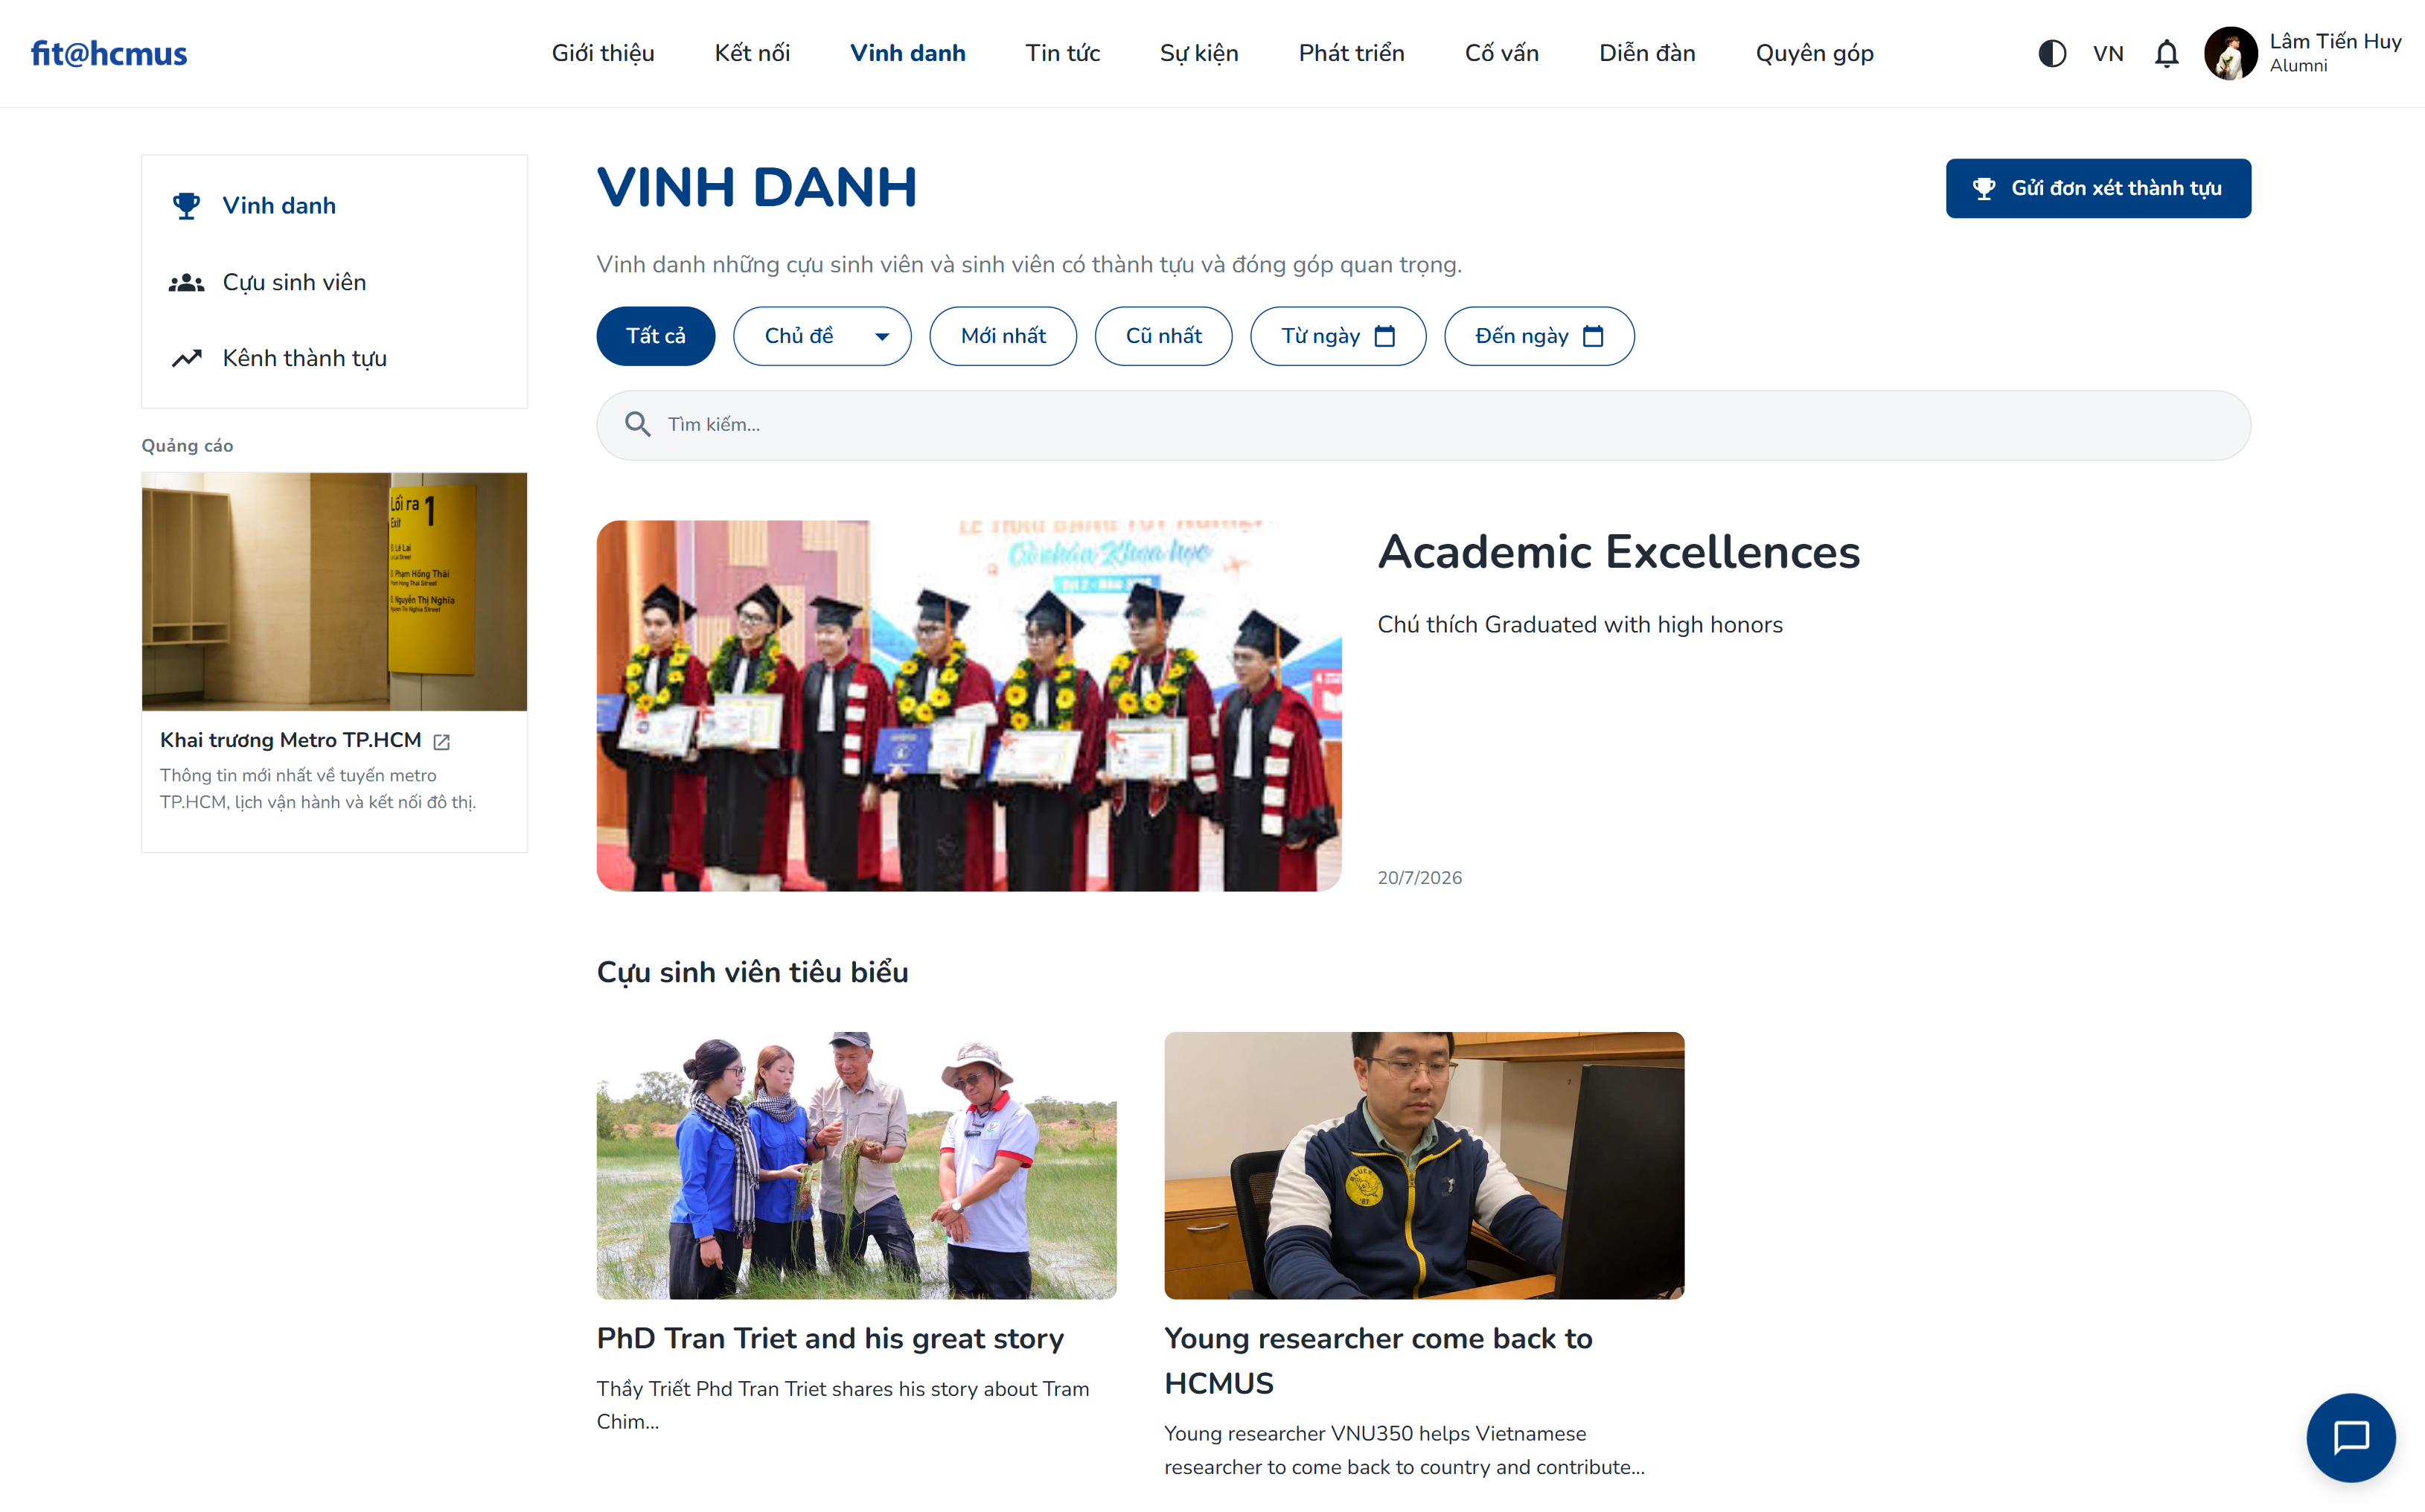
\includegraphics[width=\linewidth]{rwd-vinhdanh-desktop}\caption{Màn hình rộng: lưới nhiều cột, thanh điều hướng trải ngang}\end{subfigure}
\vspace{10pt}
\begin{subfigure}{0.545\textwidth}\centering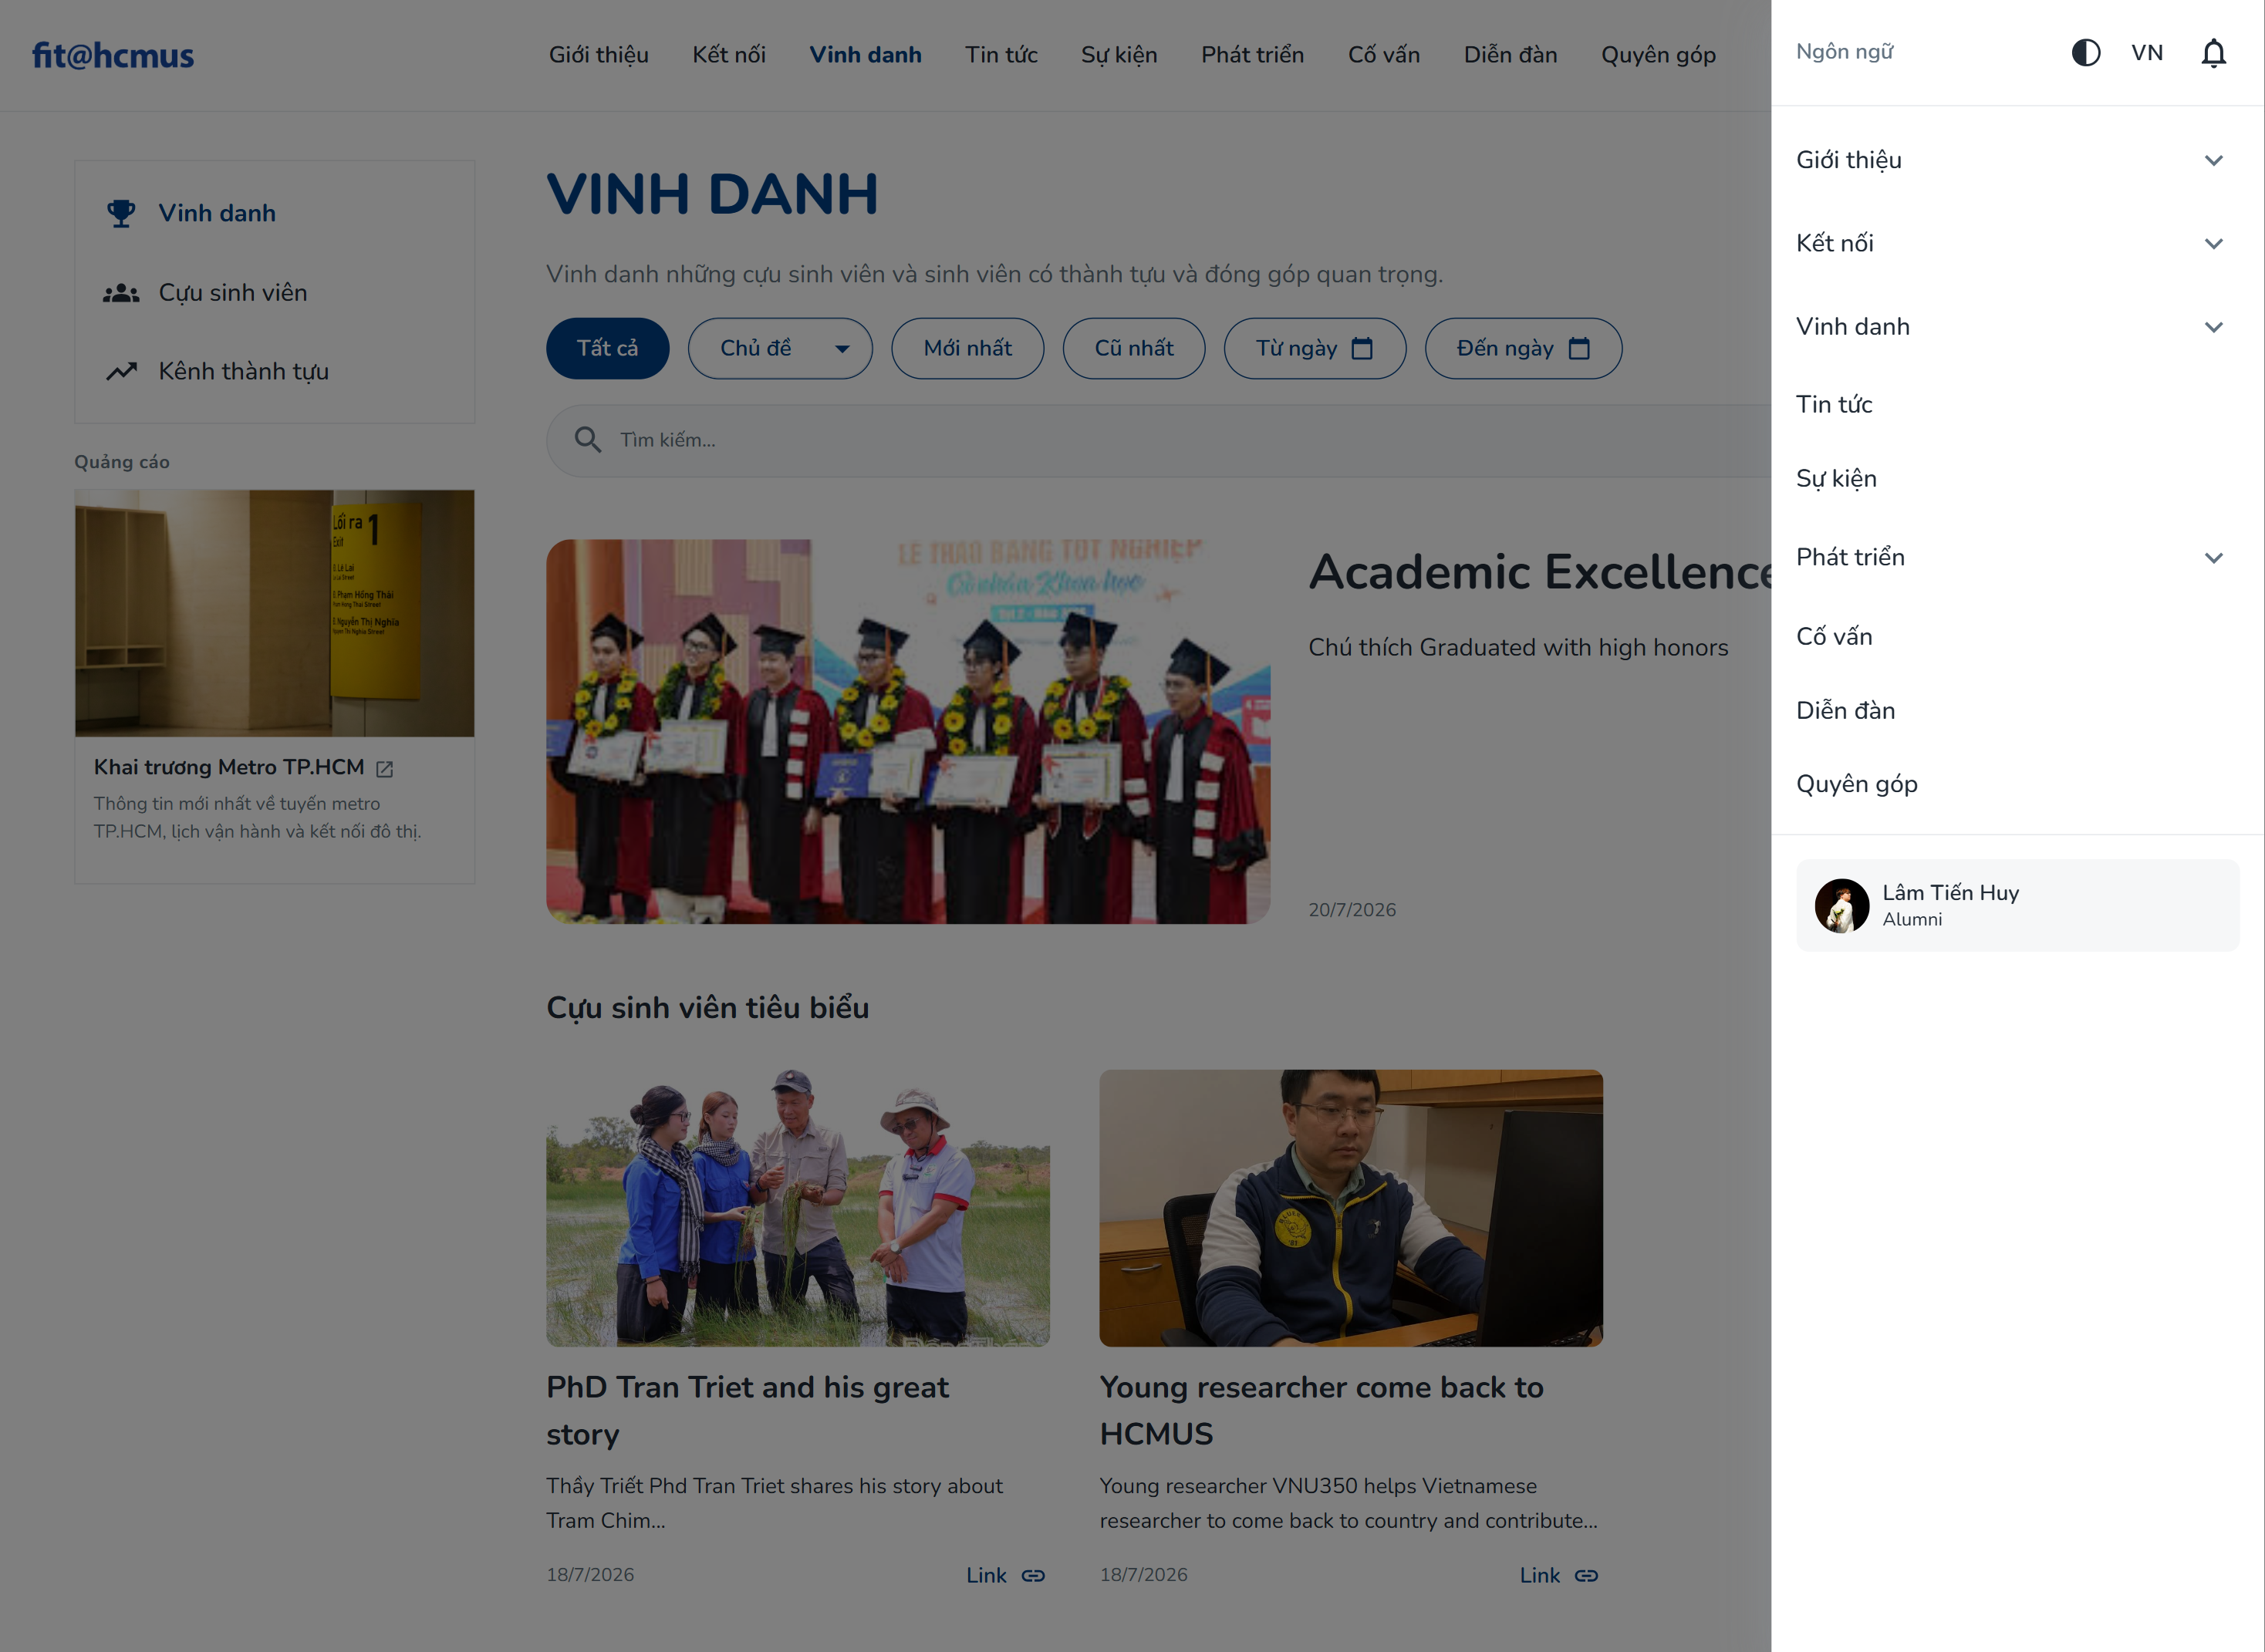
\includegraphics[width=\linewidth]{rwd-vinhdanh-tablet}\caption{Màn hình trung bình: lưới thu về ít cột, điều hướng gom vào ngăn kéo}\end{subfigure}\hfill
\begin{subfigure}{0.235\textwidth}\centering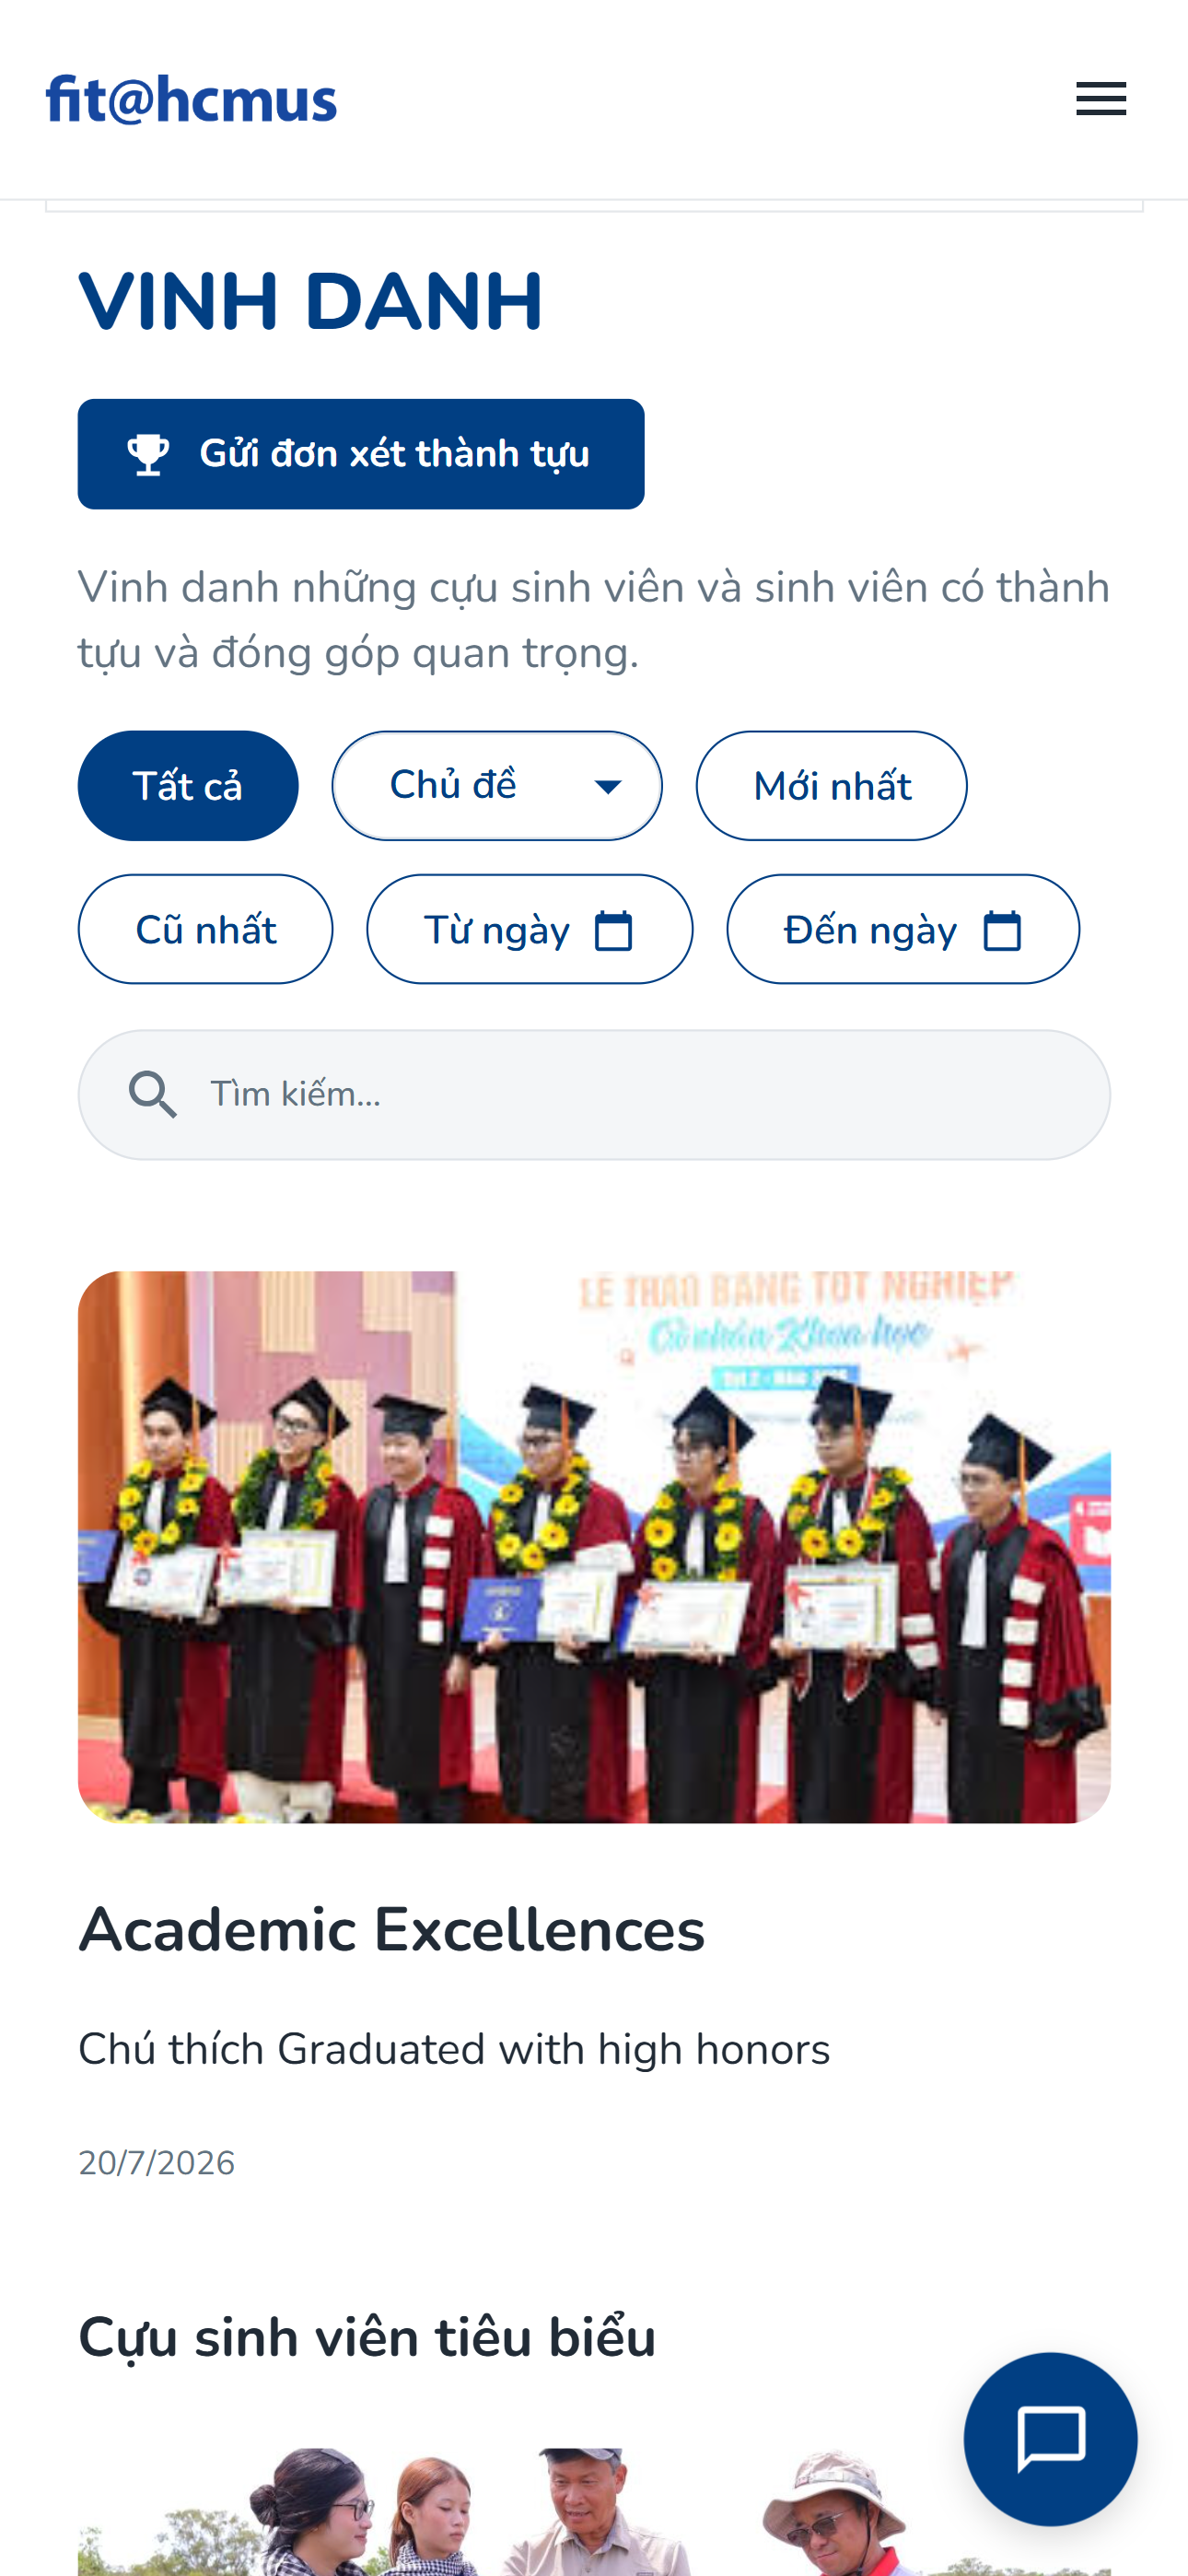
\includegraphics[width=\linewidth]{rwd-vinhdanh-mobile}\caption{Màn hình hẹp: một cột}\end{subfigure}
\caption{Cùng một trang vinh danh thành tích hiển thị trên ba nhóm kích thước màn hình}
\label{fig:responsive}
\end{figure}

\begin{figure}[H]\centering
\begin{subfigure}{\textwidth}\centering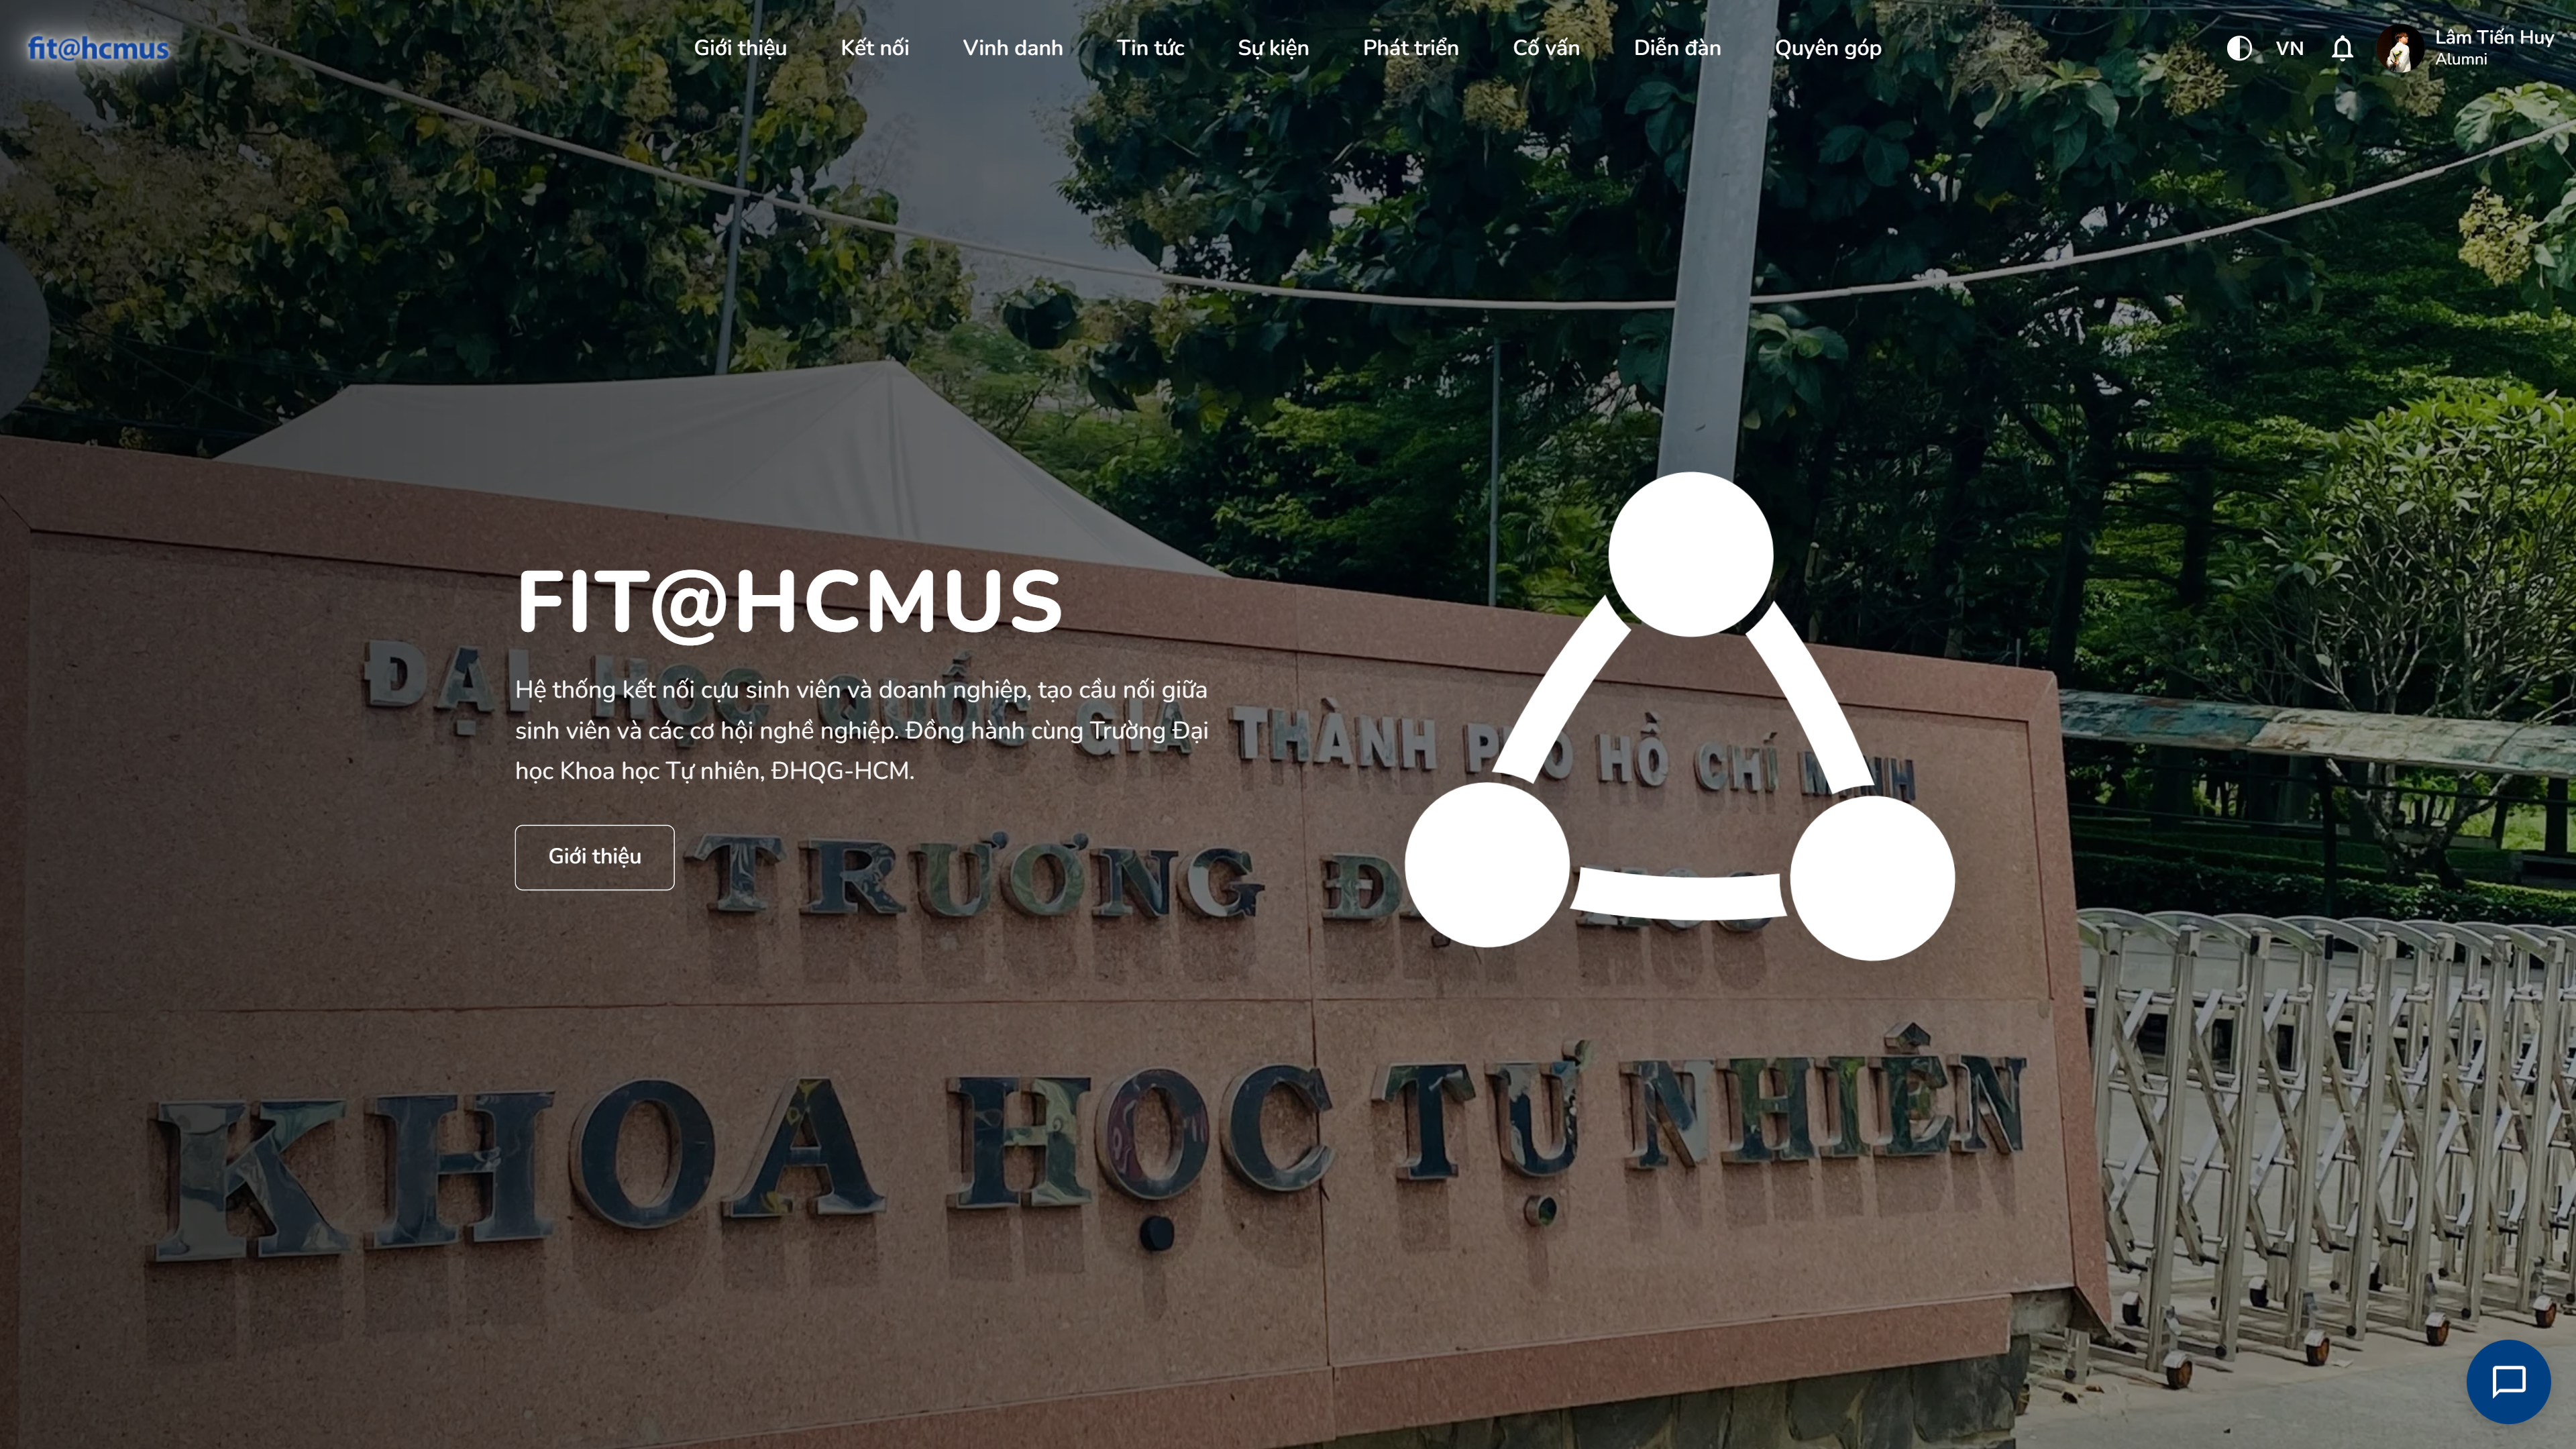
\includegraphics[width=\linewidth]{web-trang-chu}\caption{Trang chủ của một đơn vị}\end{subfigure}
\vspace{10pt}
\begin{subfigure}{\textwidth}\centering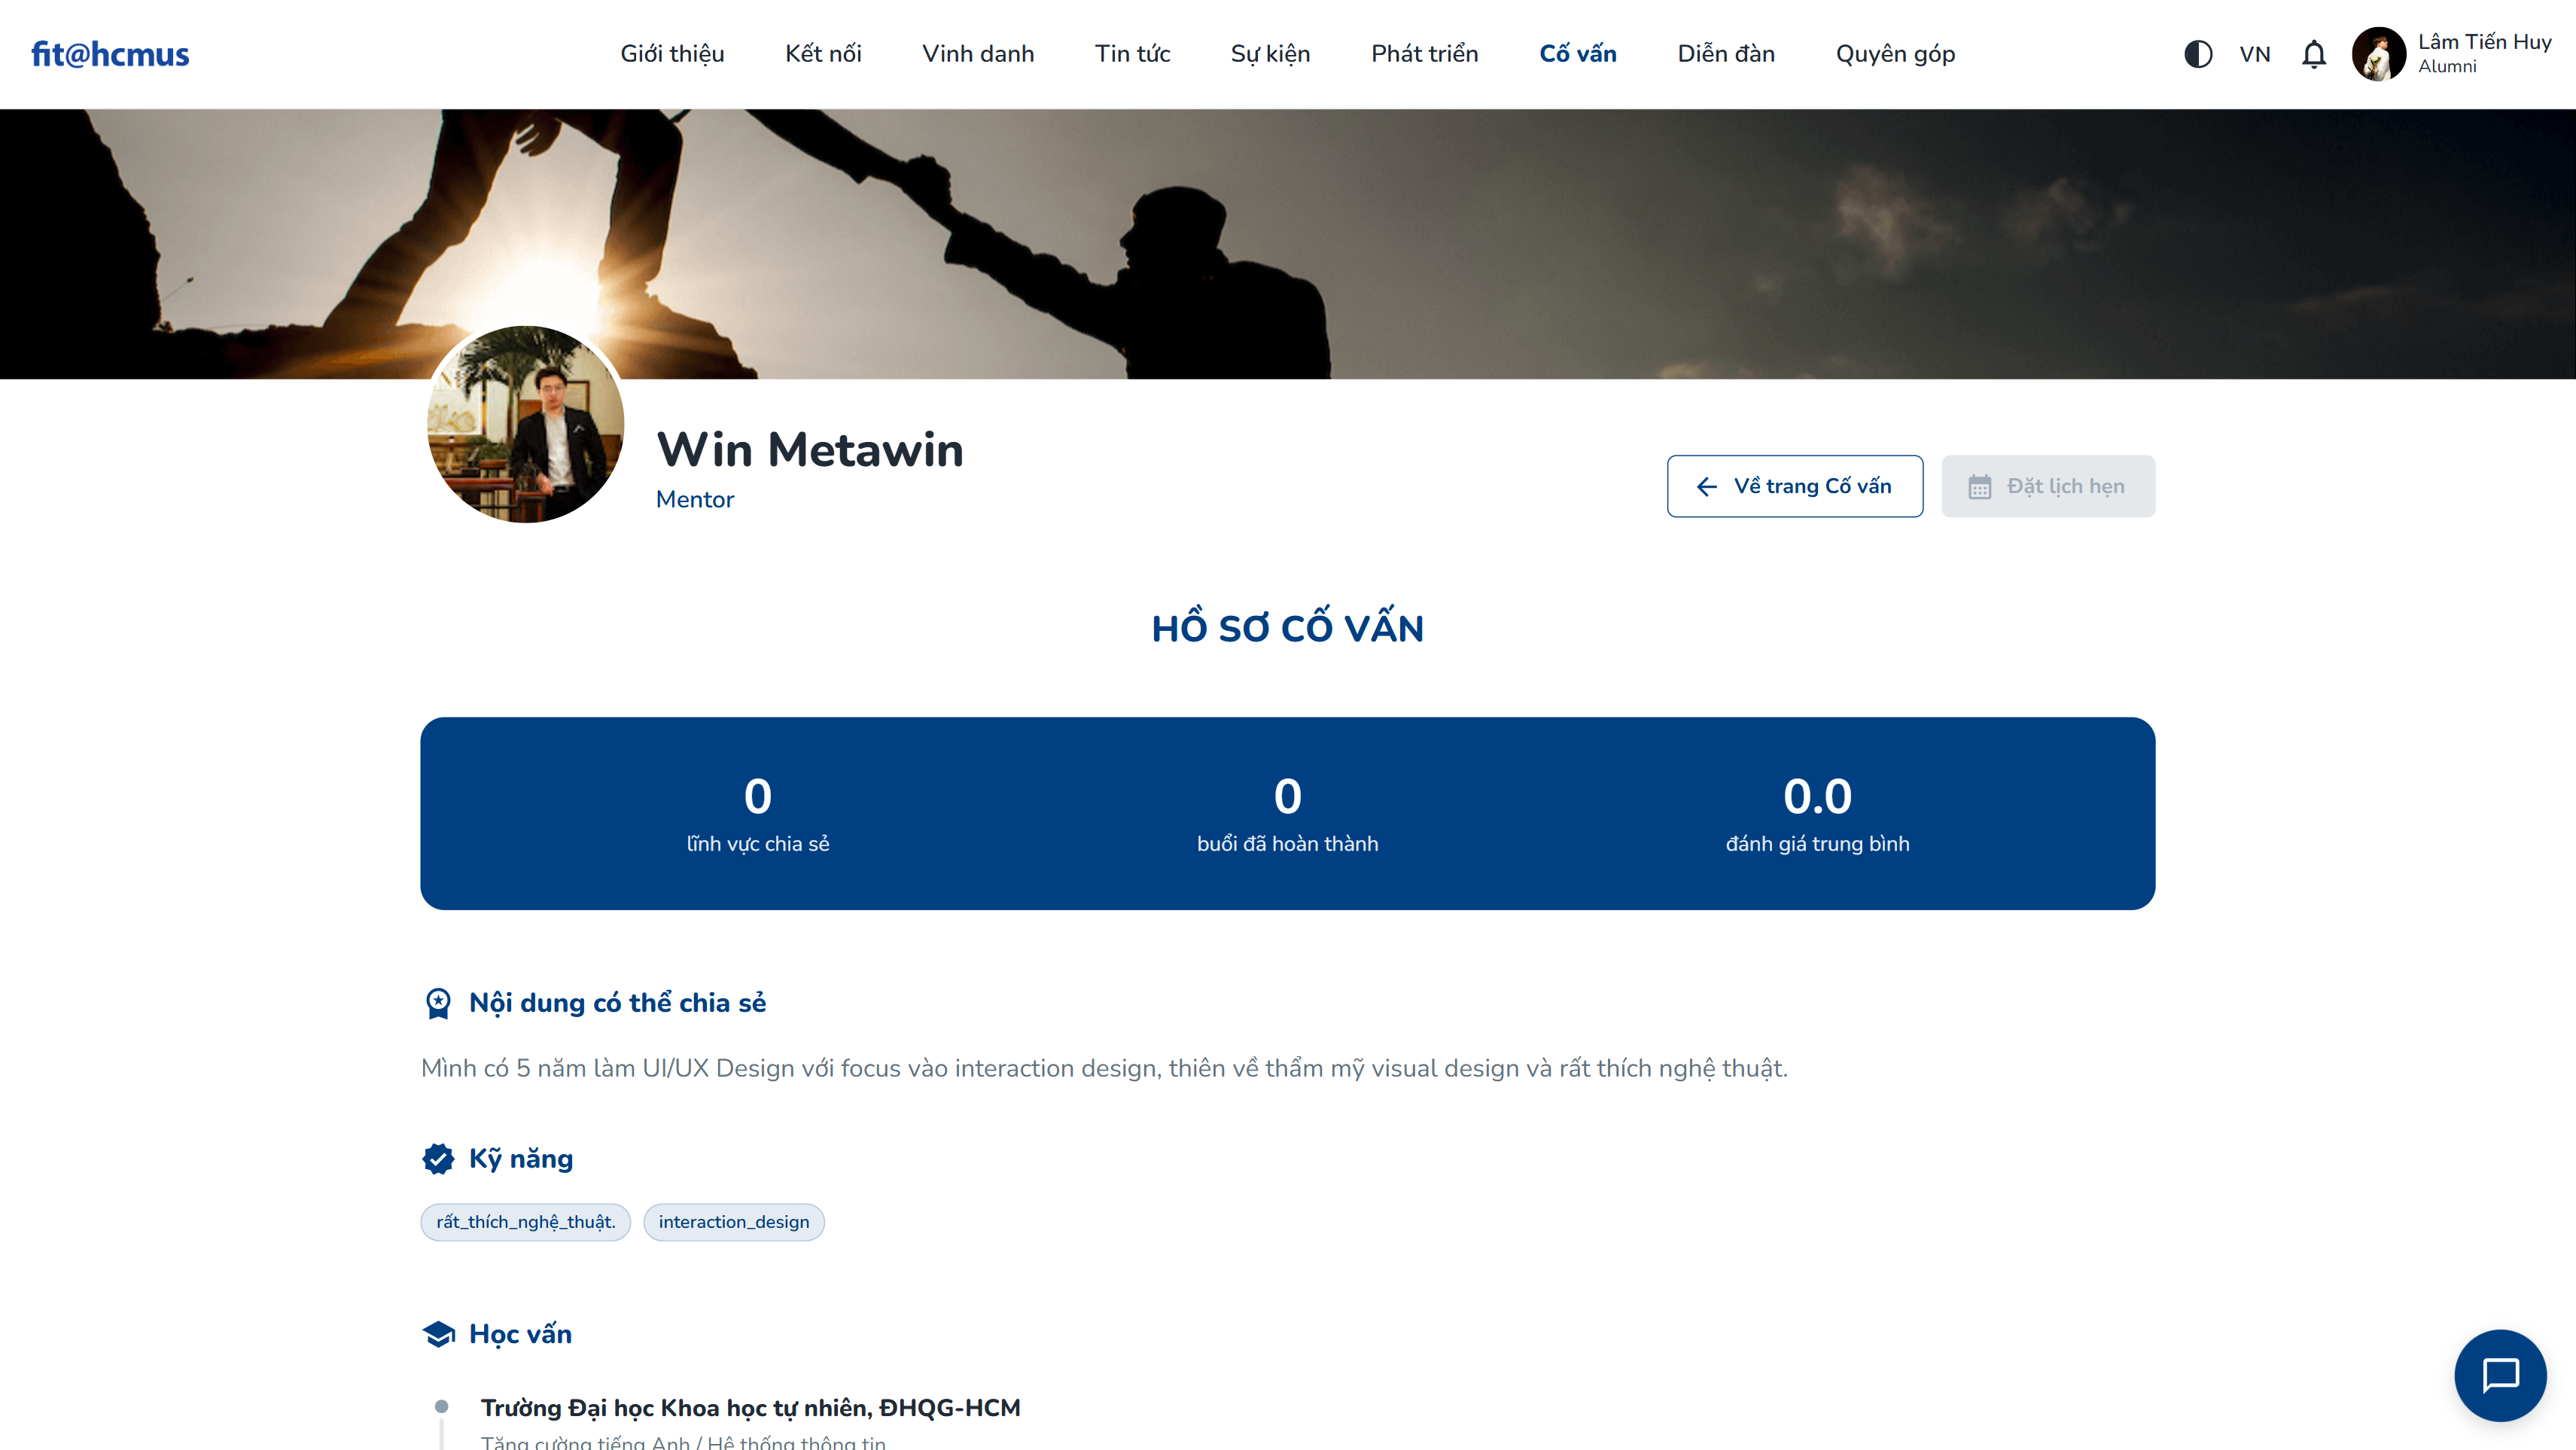
\includegraphics[width=\linewidth]{web-co-van}\caption{Danh sách người cố vấn}\end{subfigure}
\caption{Màn hình trang chủ và danh sách người cố vấn trên ứng dụng web}
\label{fig:webscreens}
\end{figure}

\begin{figure}[H]\centering
\begin{subfigure}{\textwidth}\centering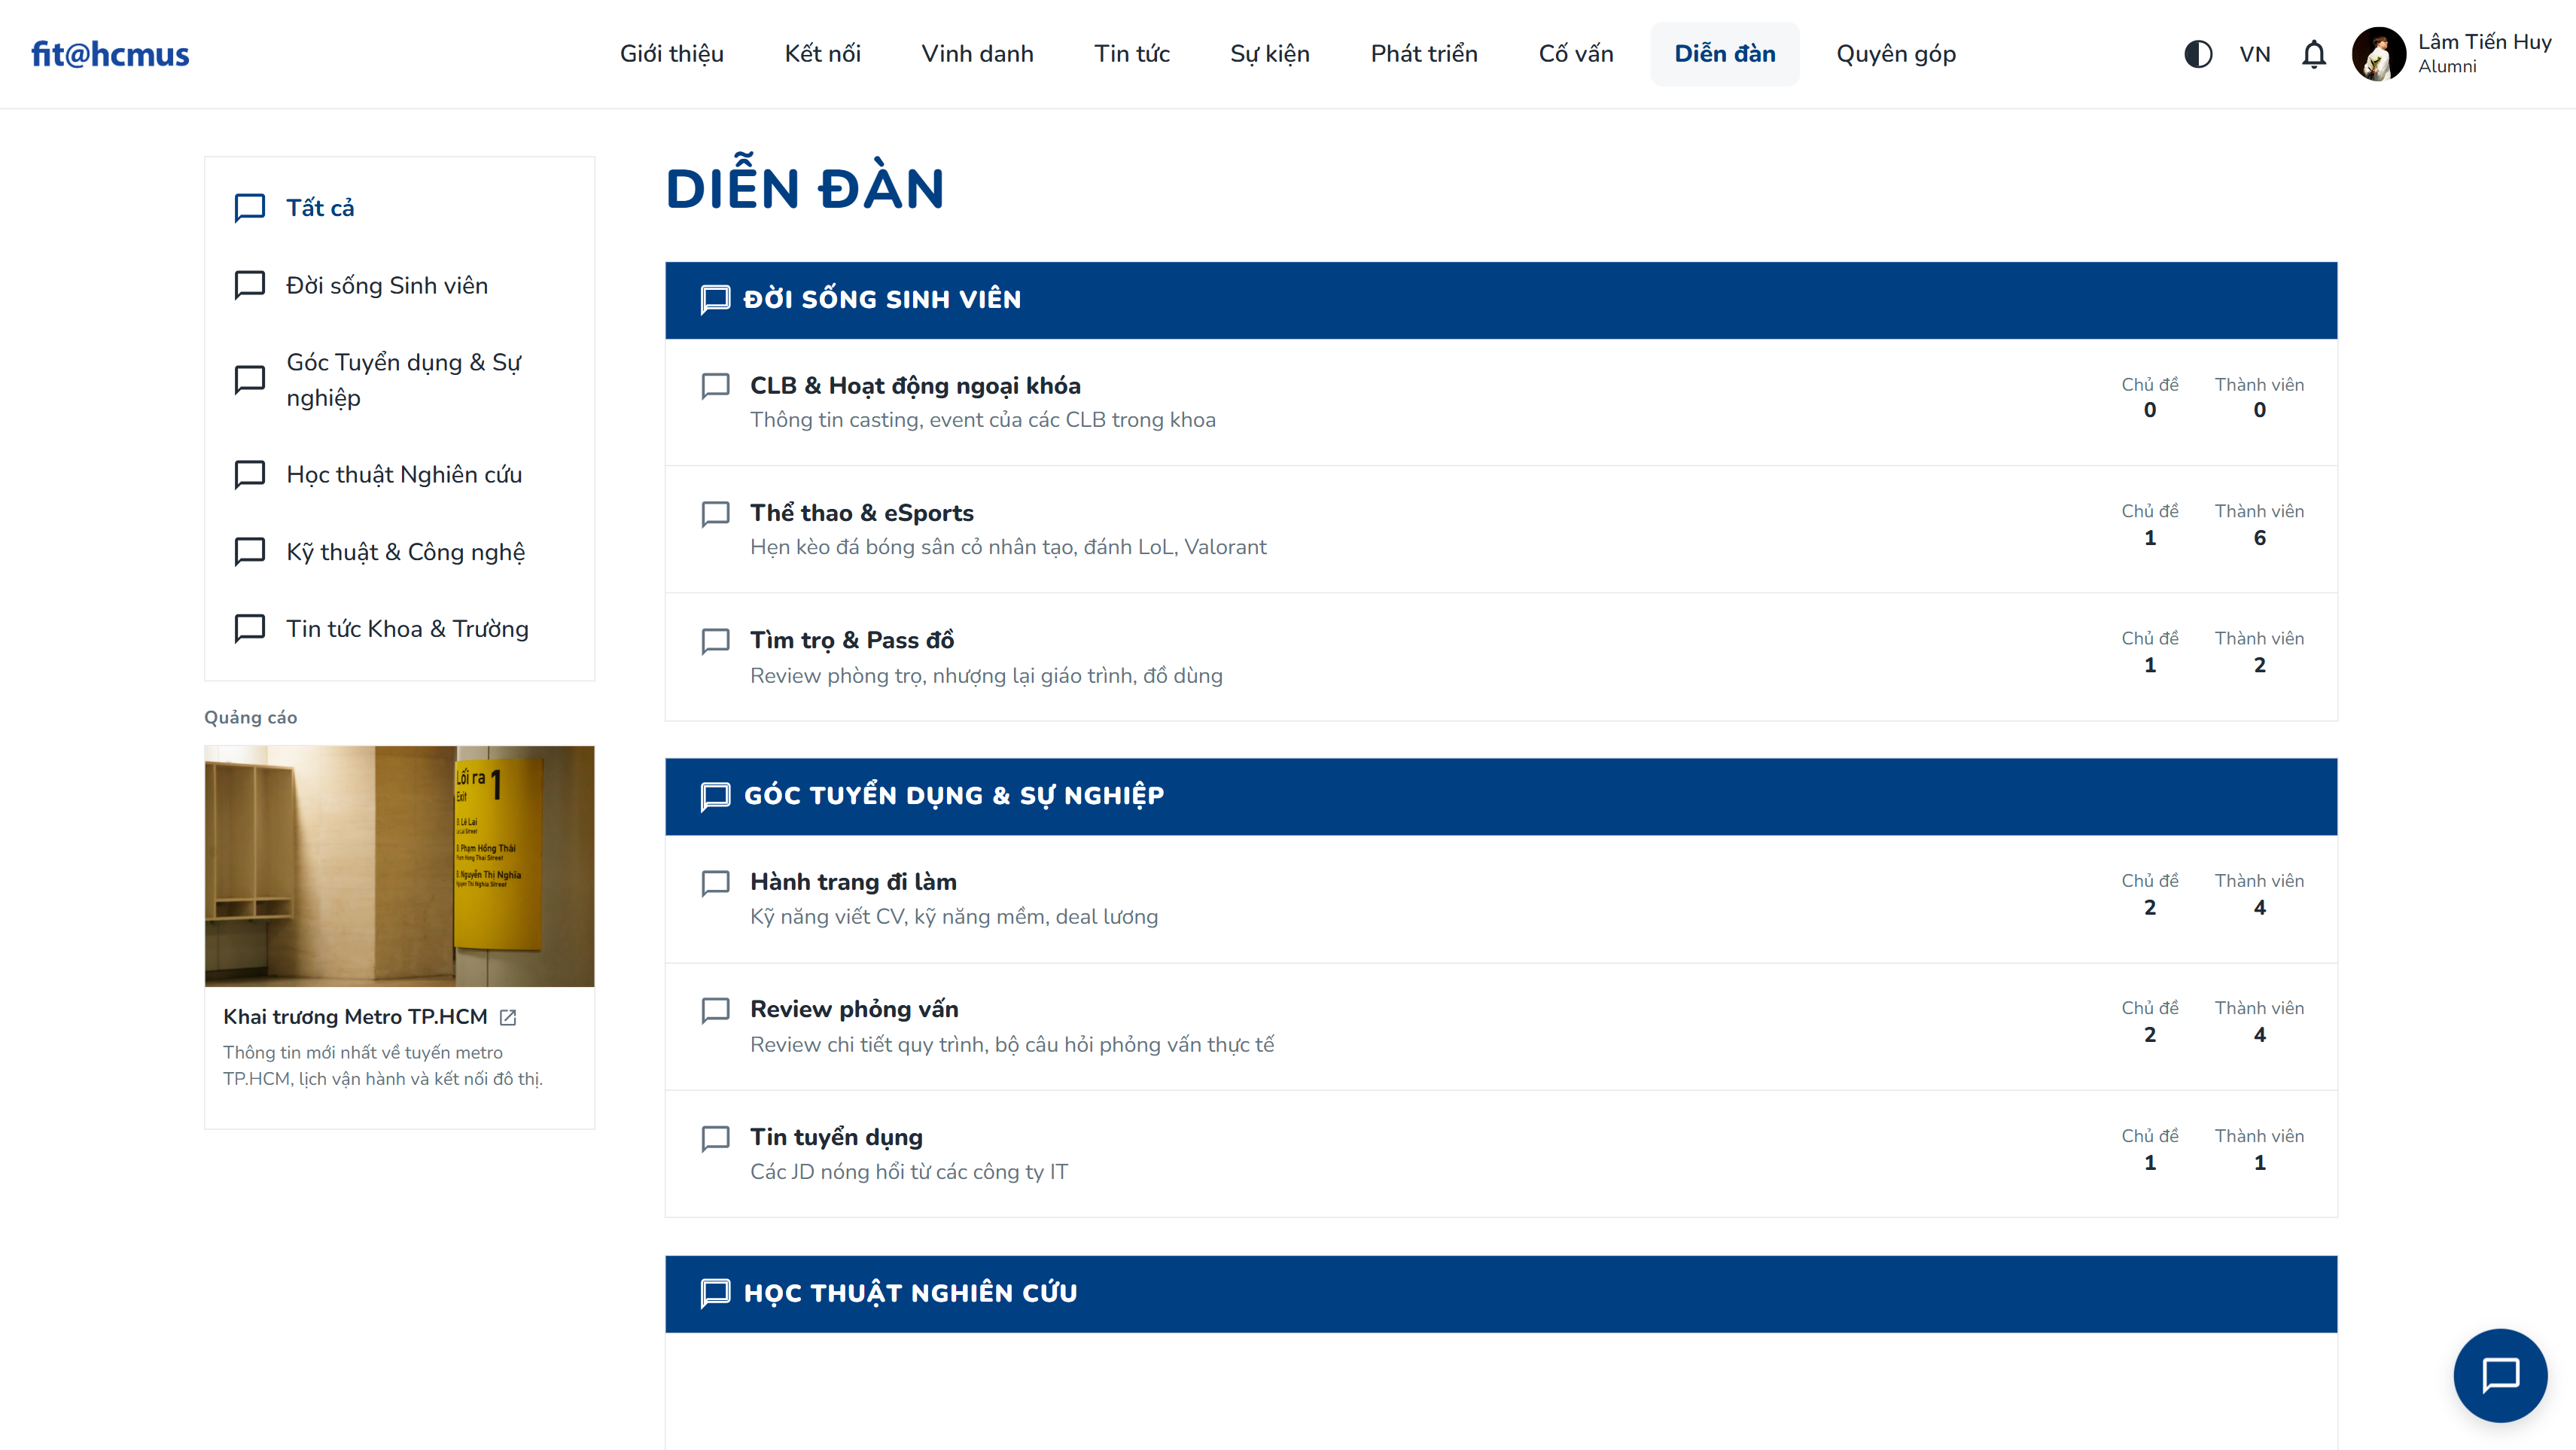
\includegraphics[width=\linewidth]{web-dien-dan}\caption{Diễn đàn nghề nghiệp}\end{subfigure}
\vspace{10pt}
\begin{subfigure}{\textwidth}\centering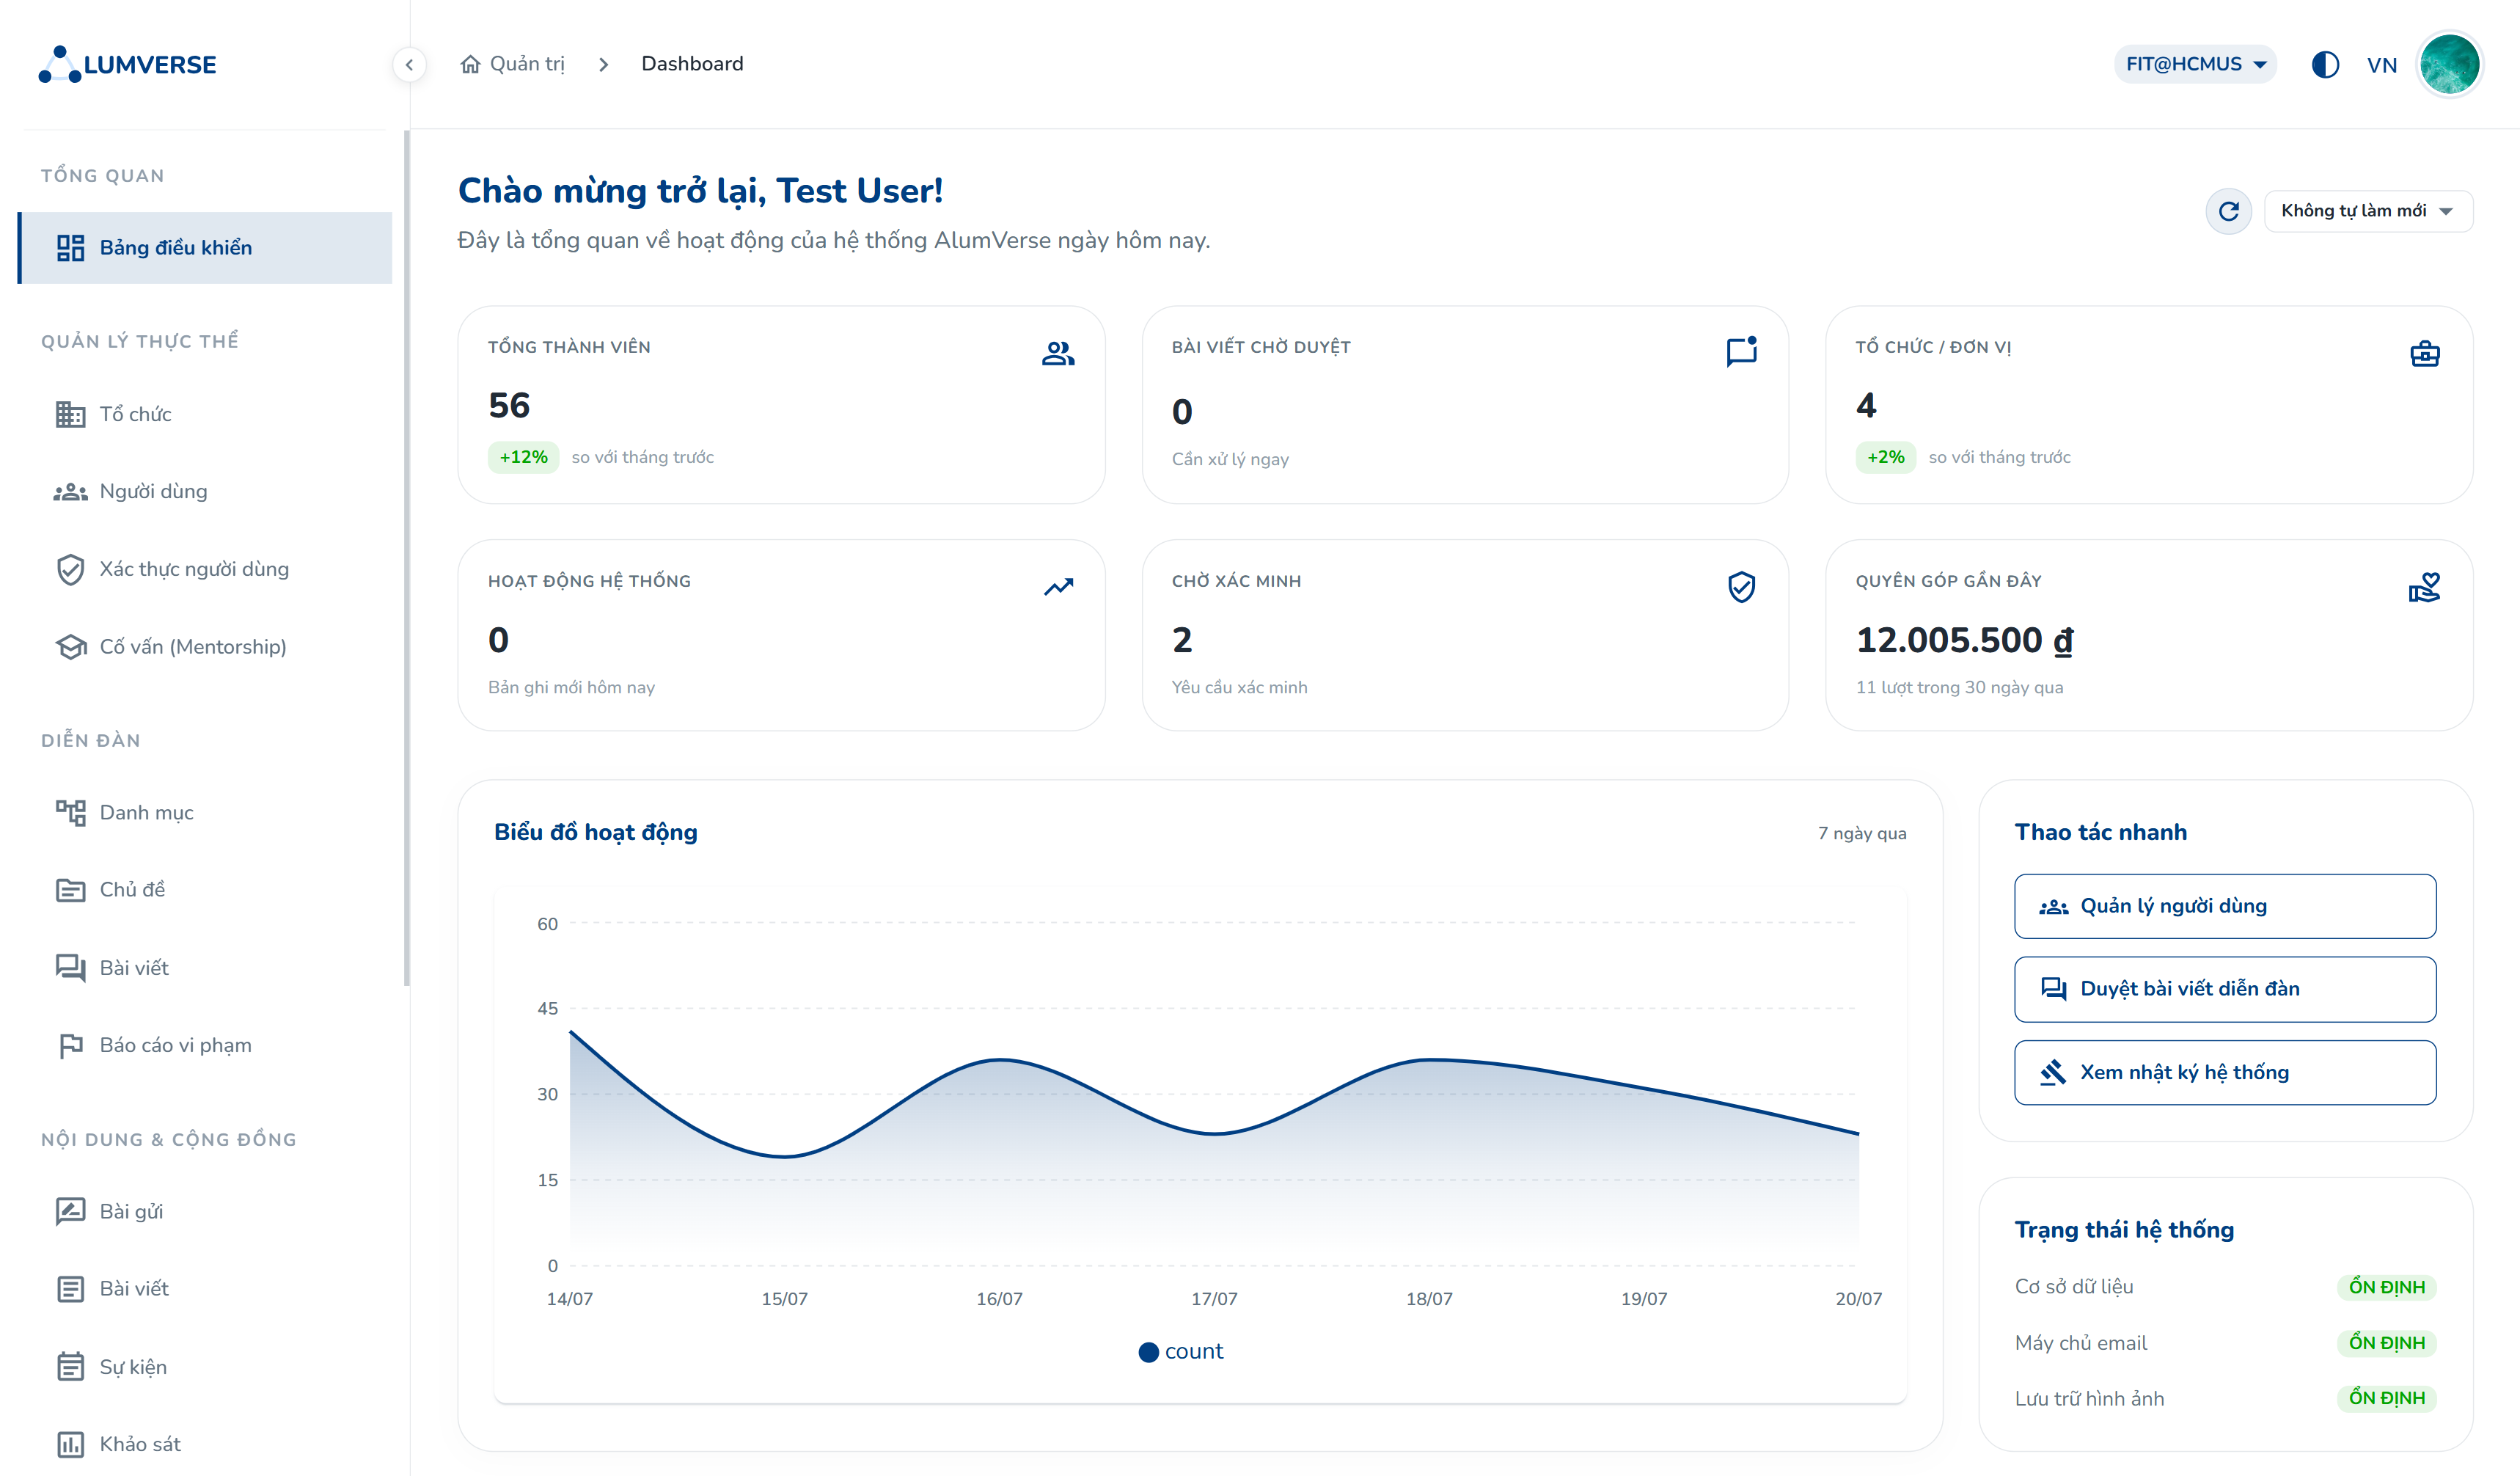
\includegraphics[width=\linewidth]{web-admin-dashboard}\caption{Bảng điều khiển quản trị đơn vị}\end{subfigure}
\caption{Màn hình diễn đàn và bảng điều khiển quản trị trên ứng dụng web}
\label{fig:webscreens2}
\end{figure}

\subsection{Ứng dụng di động}

Ứng dụng di động được xây dựng bằng Flutter, dùng chung tầng API với ứng dụng web nên toàn bộ nghiệp vụ được thống nhất ở một nơi duy nhất, tránh tình trạng hai nền tảng hiểu khác nhau về cùng một quy tắc.

Ứng dụng quản lý trạng thái bằng Riverpod, điều hướng bằng go\_router và gọi API bằng Dio. Do đặc thù thiết bị di động, ứng dụng ưu tiên các luồng nghiệp vụ thường dùng khi di chuyển như xem tin tức và sự kiện, nhắn tin, nhận thông báo, và đặc biệt là điểm danh sự kiện bằng mã QR dành cho đội ngũ giáo vụ.

\begin{figure}[H]\centering
\begin{subfigure}{0.315\textwidth}\centering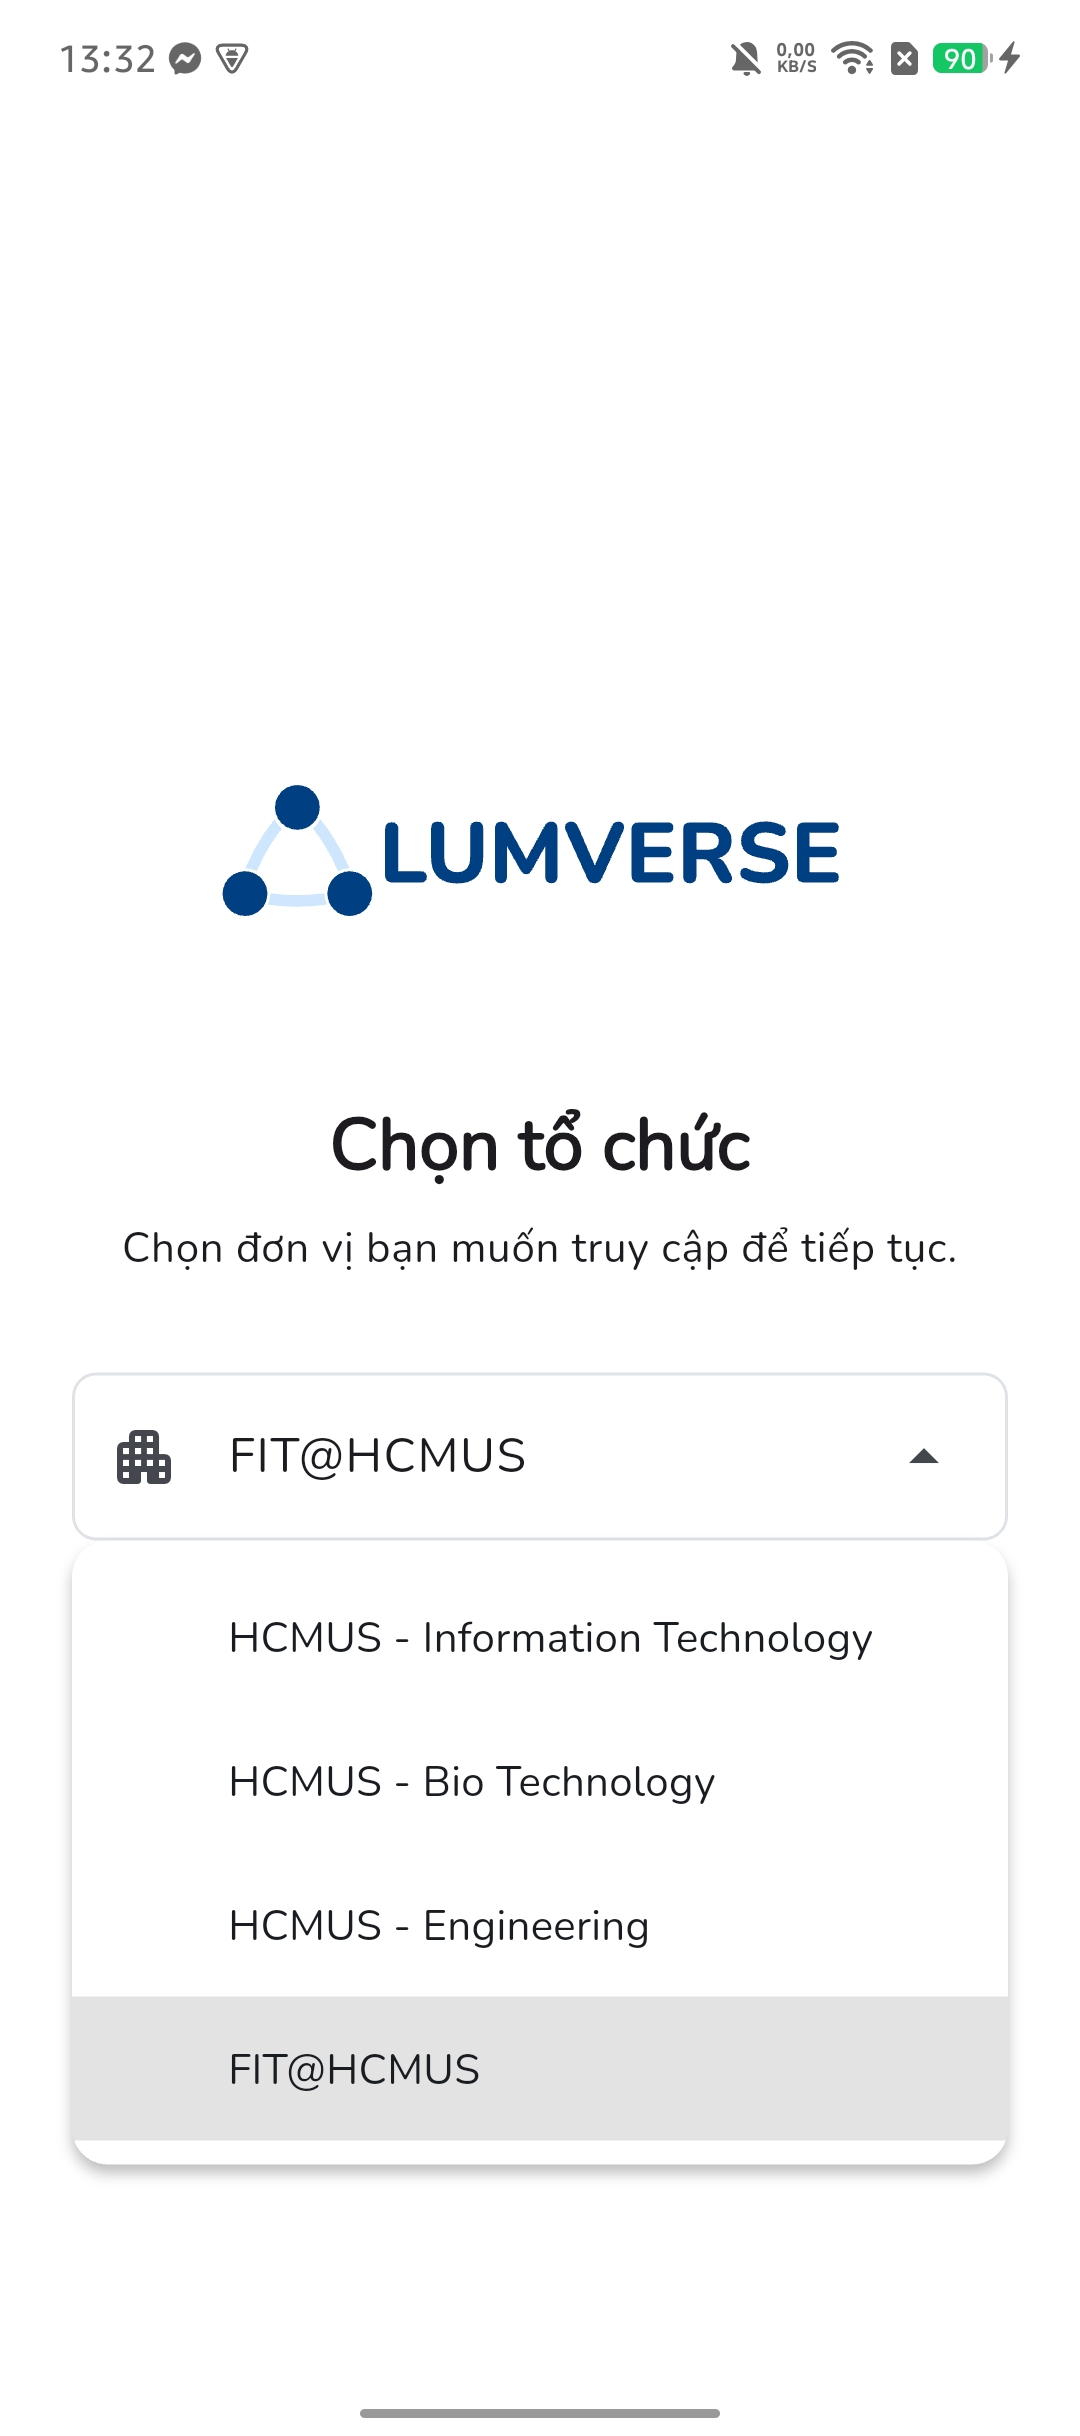
\includegraphics[width=\linewidth]{mob-01-chon-to-chuc}\caption{Chọn đơn vị}\end{subfigure}\hfill
\begin{subfigure}{0.315\textwidth}\centering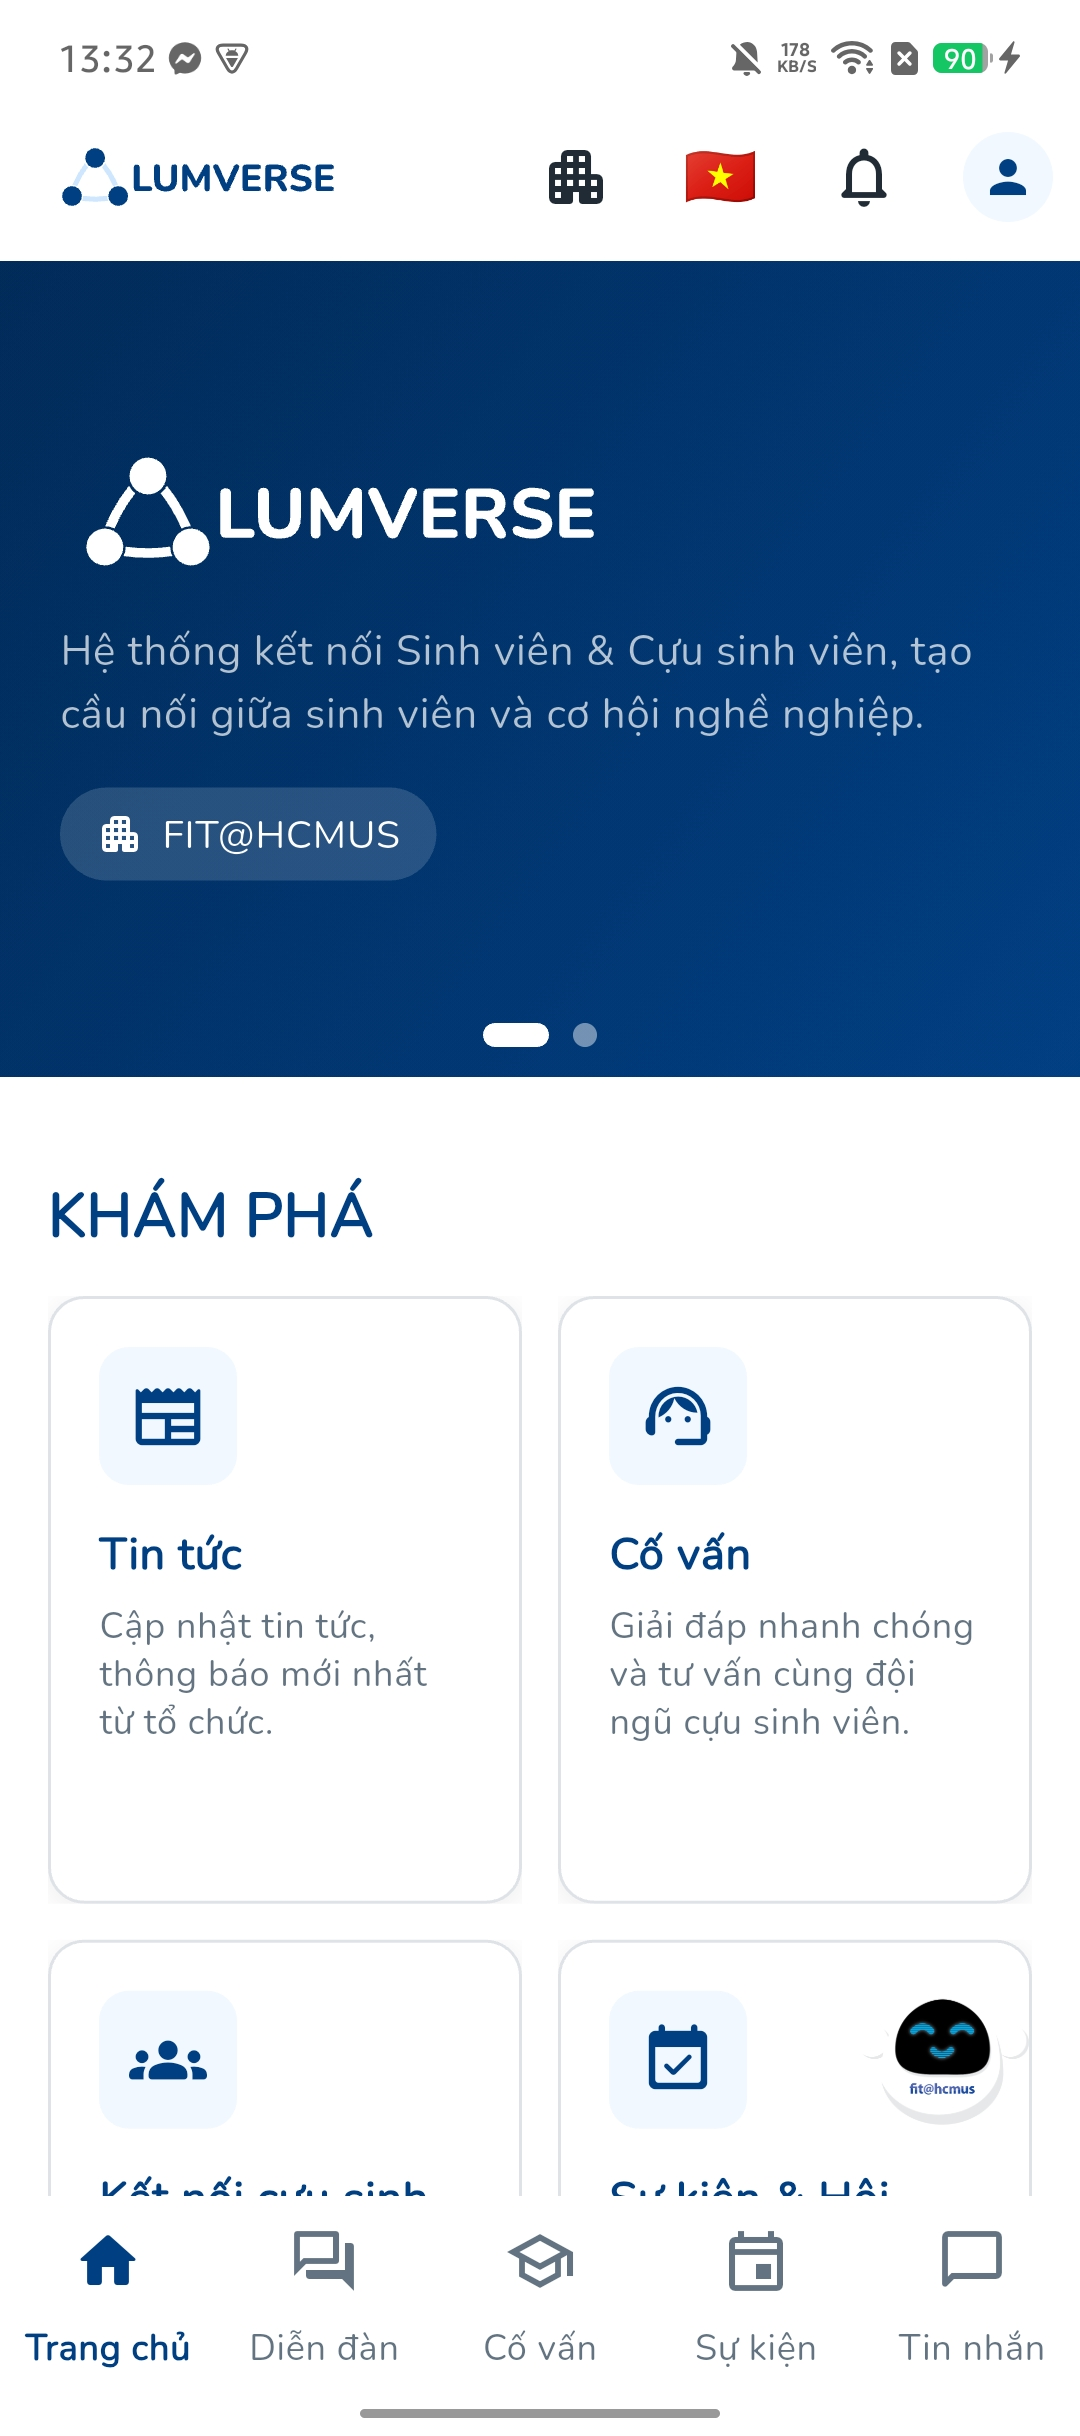
\includegraphics[width=\linewidth]{mob-02-trang-chu}\caption{Trang chủ}\end{subfigure}\hfill
\begin{subfigure}{0.315\textwidth}\centering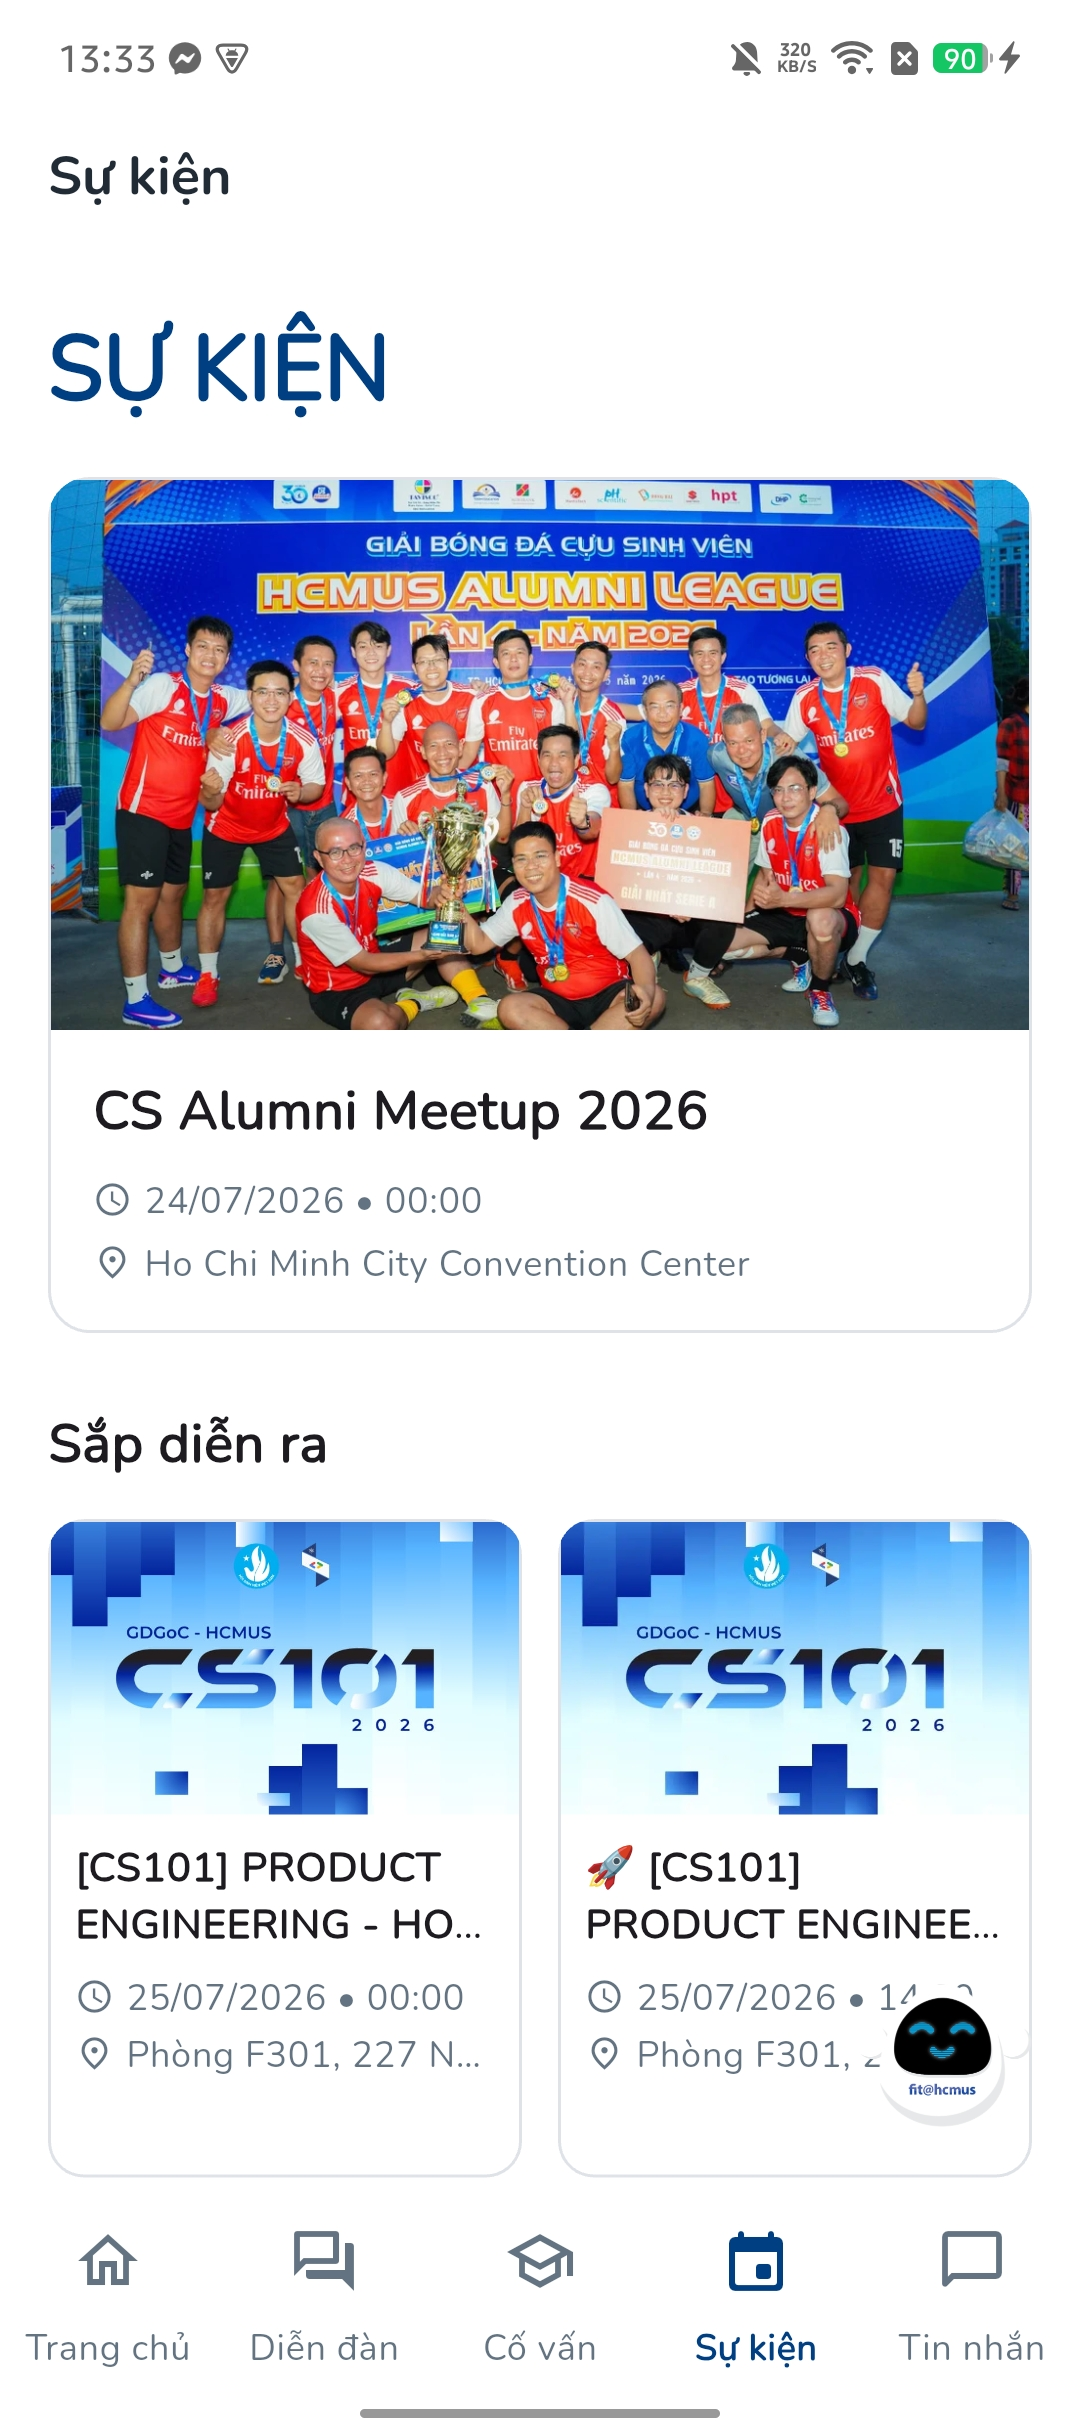
\includegraphics[width=\linewidth]{mob-04-su-kien}\caption{Danh sách sự kiện}\end{subfigure}
\caption{Màn hình chọn đơn vị, trang chủ và danh sách sự kiện trên ứng dụng di động}
\label{fig:mobilescreens}
\end{figure}

\begin{figure}[H]\centering
\begin{subfigure}{0.315\textwidth}\centering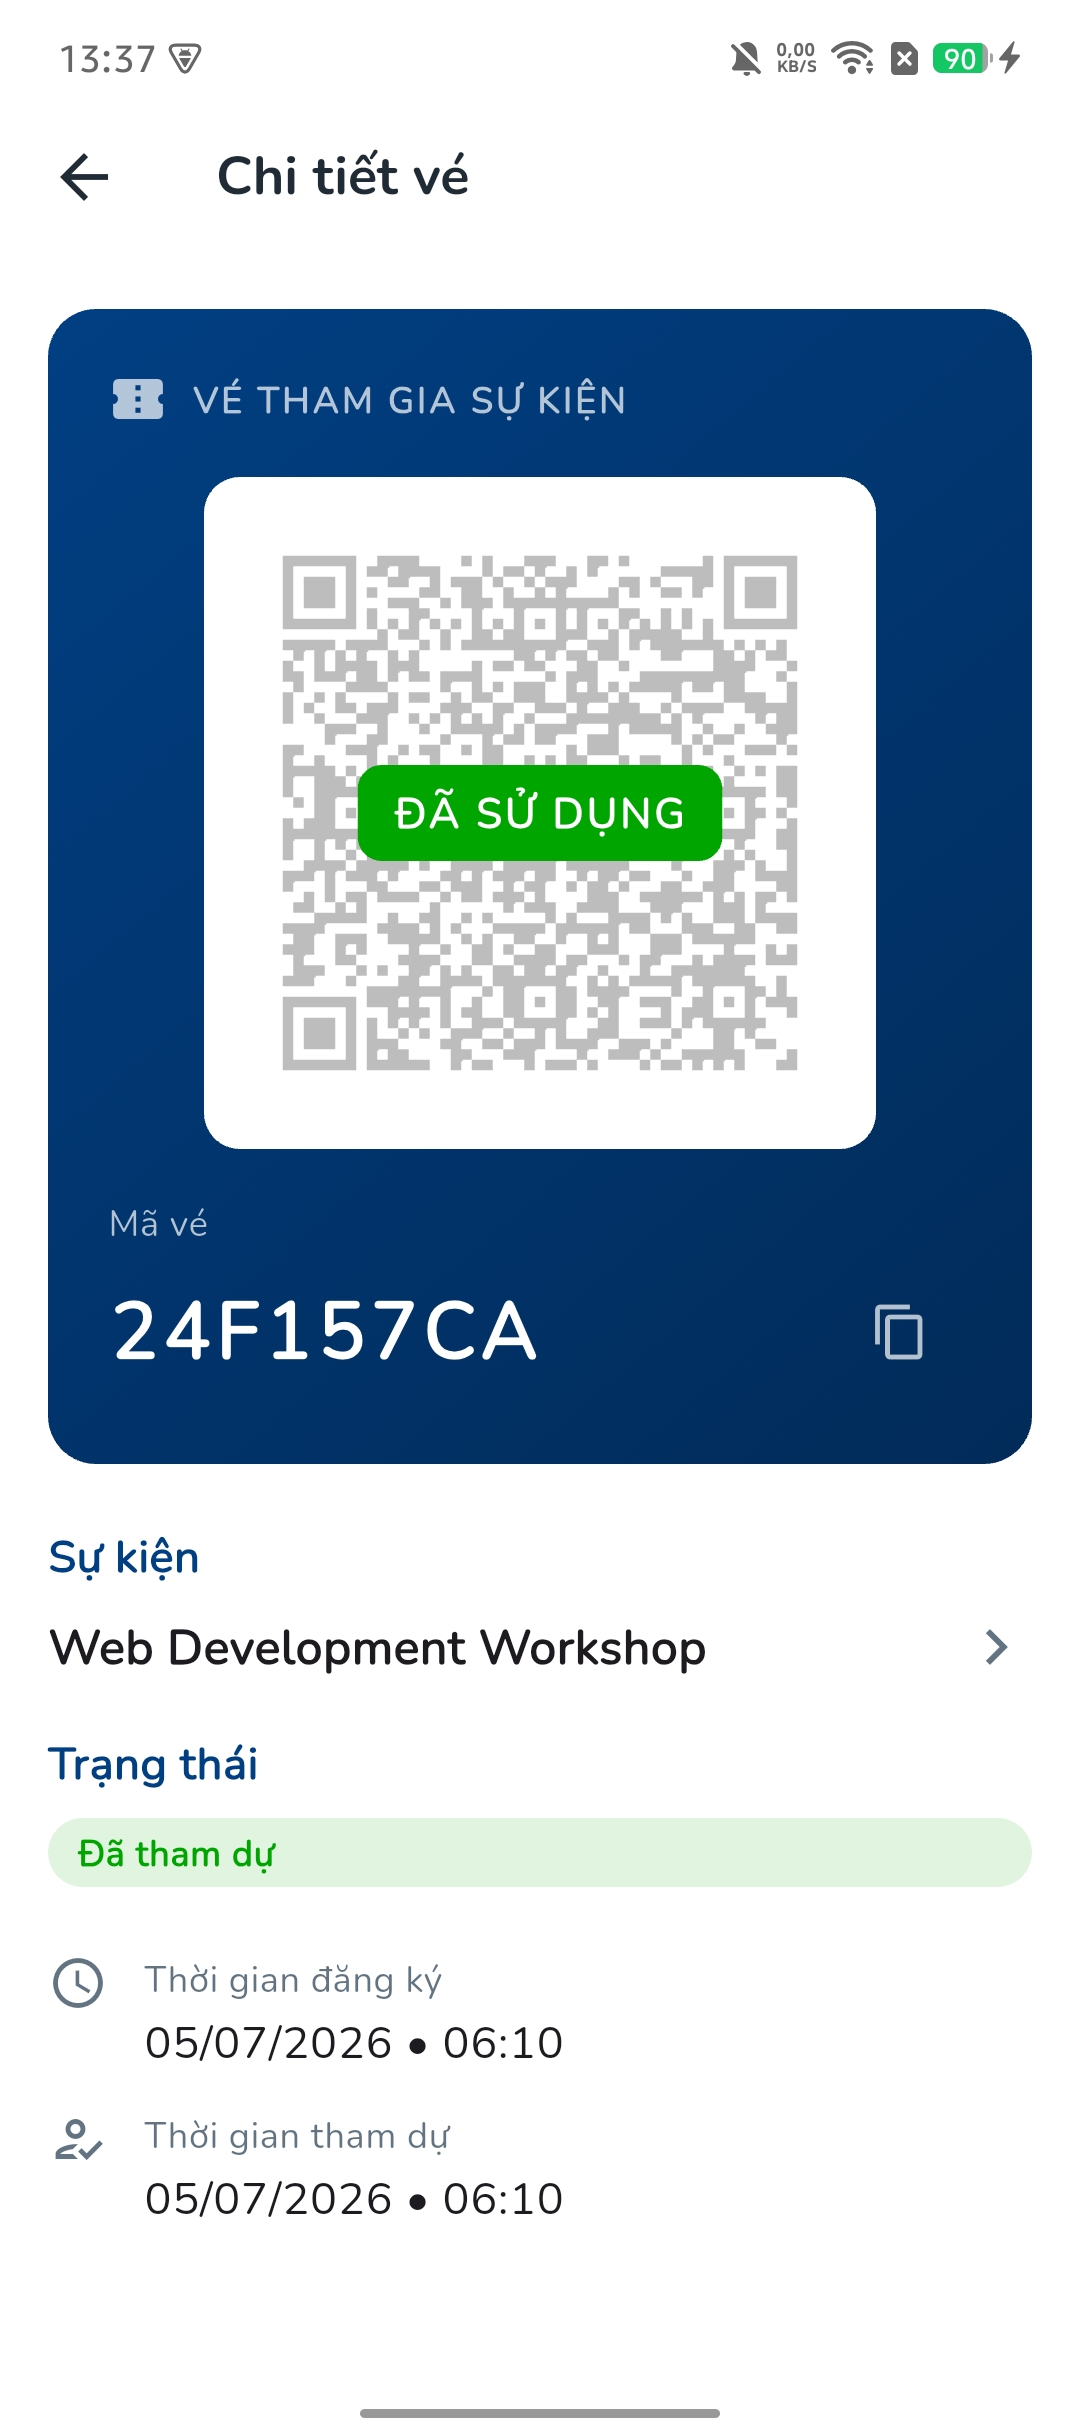
\includegraphics[width=\linewidth]{mob-05-ve-qr}\caption{Vé điện tử kèm mã QR}\end{subfigure}\hfill
\begin{subfigure}{0.315\textwidth}\centering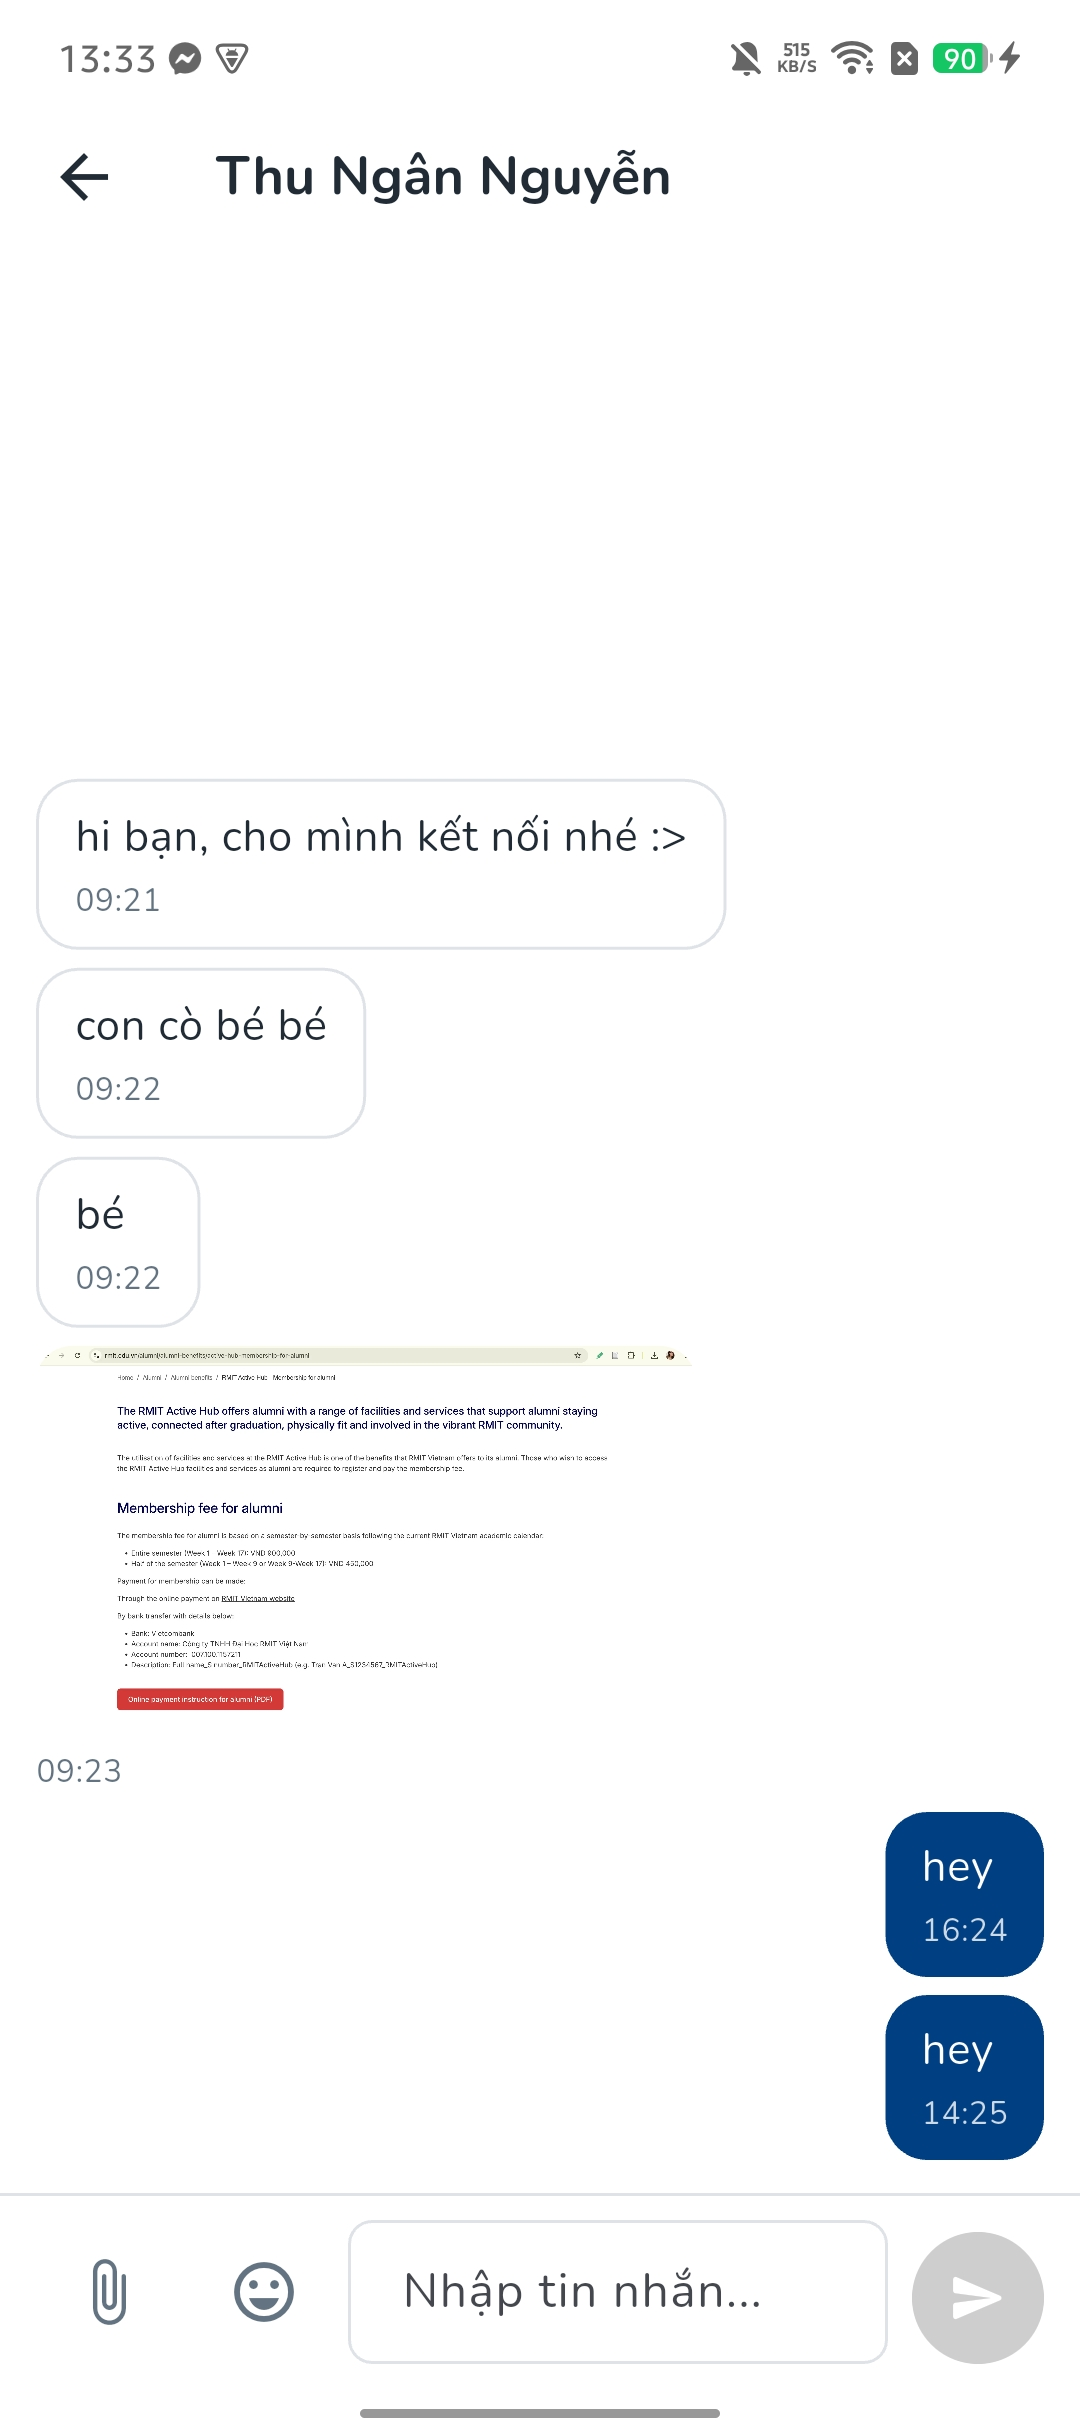
\includegraphics[width=\linewidth]{mob-06-chat}\caption{Hội thoại nhắn tin}\end{subfigure}\hfill
\begin{subfigure}{0.315\textwidth}\centering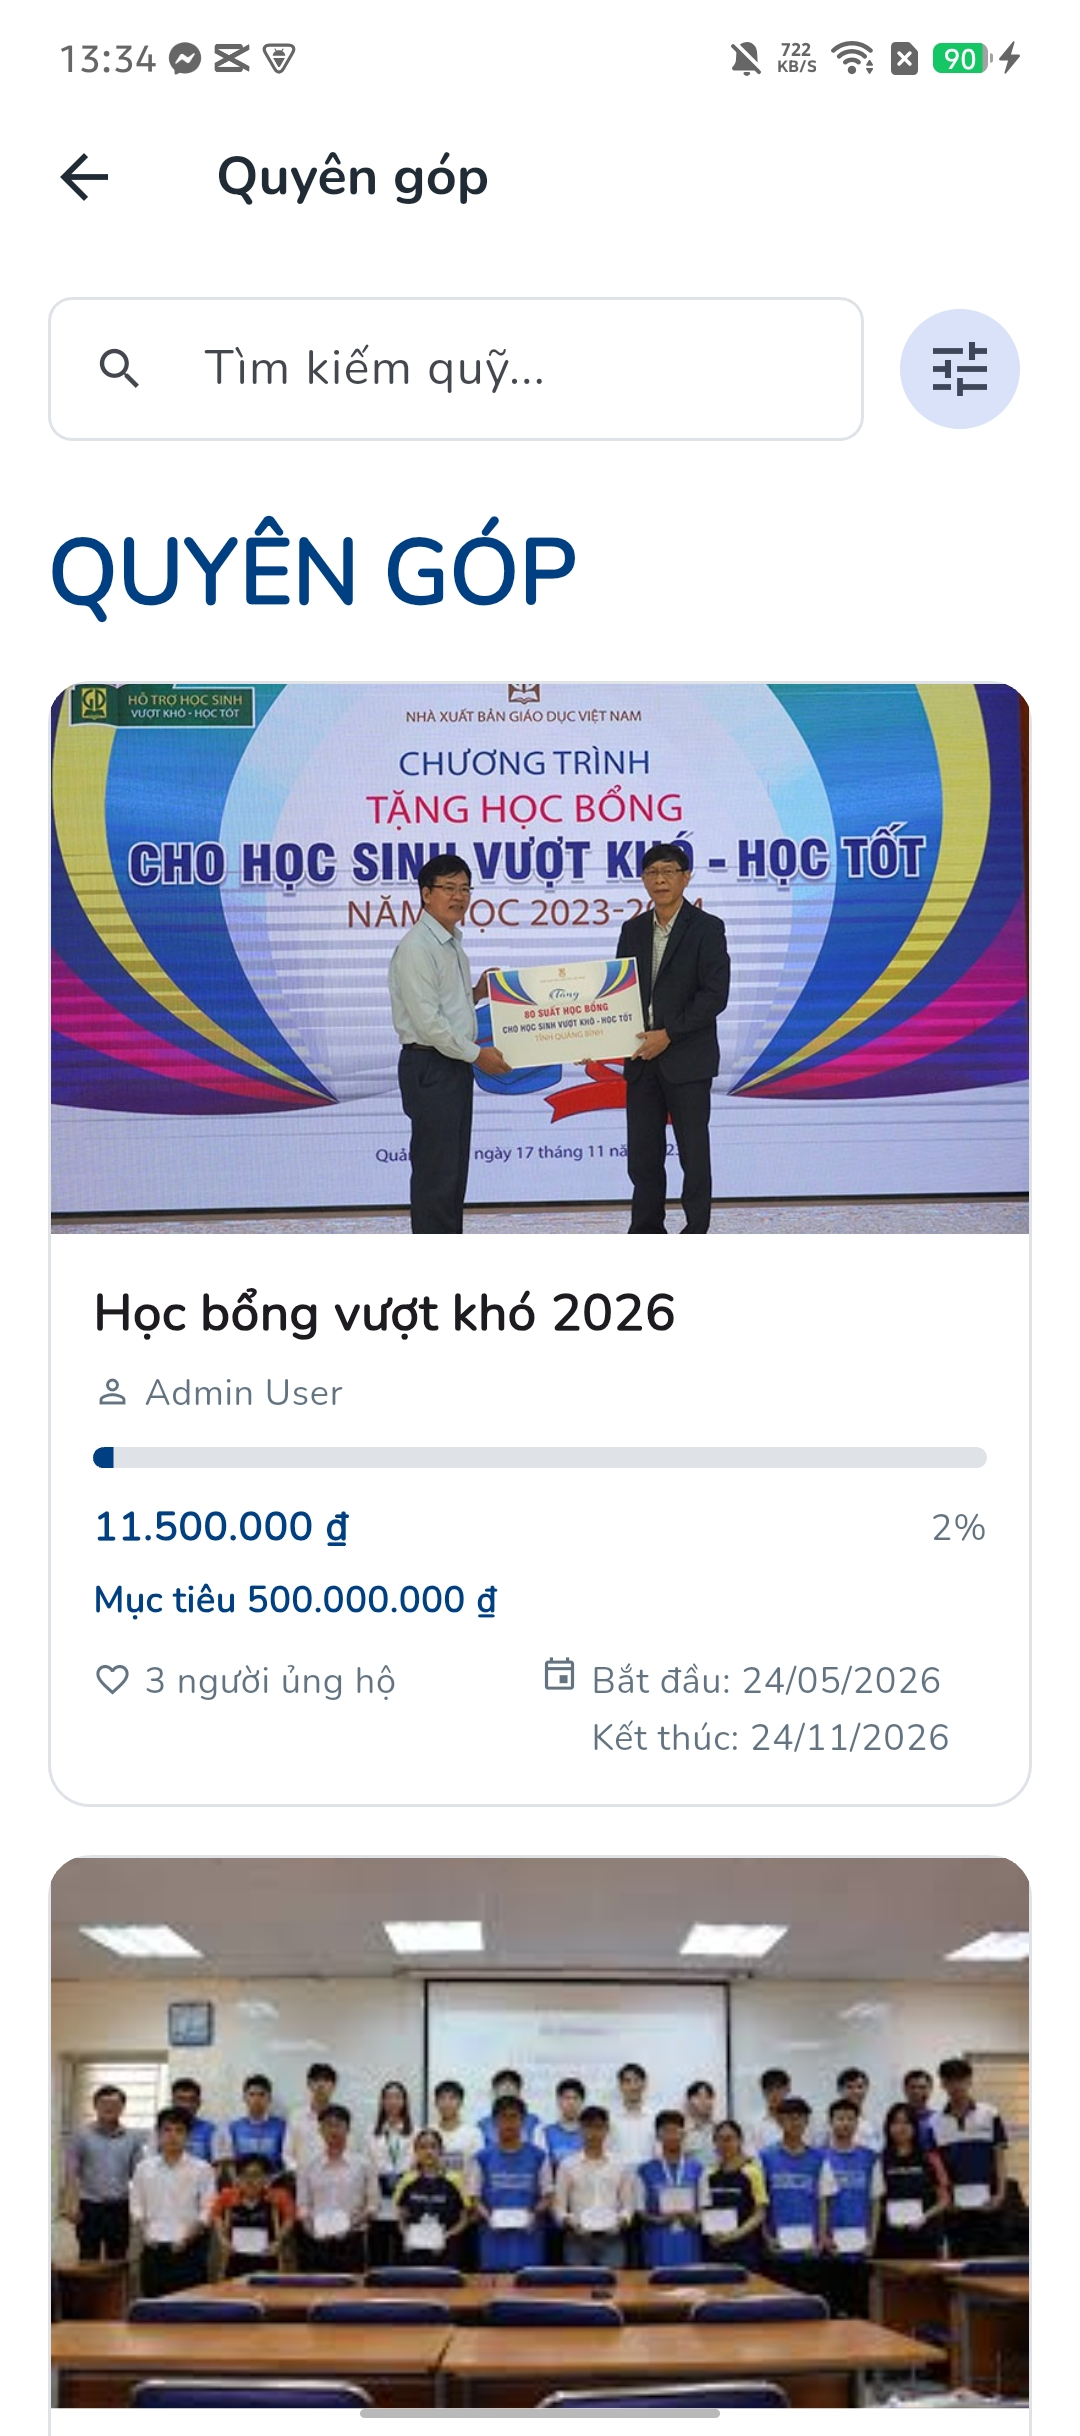
\includegraphics[width=\linewidth]{mob-08-quyen-gop}\caption{Danh sách quỹ quyên góp}\end{subfigure}
\caption{Màn hình vé điện tử, nhắn tin và quyên góp trên ứng dụng di động}
\label{fig:mobilescreens2}
\end{figure}

\subsection{Sơ đồ tuần tự các luồng tiêu biểu}

Hai luồng nghiệp vụ được chọn mô tả bằng sơ đồ tuần tự là đặt lịch cố vấn và đóng góp quỹ kèm đối soát giao dịch. Đây cũng chính là hai luồng được nêu như trọng tâm nghiệp vụ của đề tài, vì mỗi luồng đều mang một ràng buộc kỹ thuật không thể xử lý bằng thao tác ghi thông thường: một bên là tranh chấp khi nhiều người cùng đặt một khung giờ, một bên là thông báo lặp từ cổng thanh toán. Sơ đồ tuần tự làm rõ thứ tự tương tác giữa người dùng, giao diện, các tầng phía máy chủ và cơ sở dữ liệu, đồng thời chỉ ra chính xác vị trí đặt cơ chế kiểm soát.

Luồng nhắn tin thời gian thực và mạng lưới kết nối được mô tả ở mục 4.4.4 kèm sơ đồ tuần tự riêng.

\begin{figure}[H]\centering
\begin{tikzpicture}[font=\small,
 hdr/.style={draw,fill=blue!10,rounded corners=2pt,minimum height=8mm,text width=27mm,align=center,inner sep=2pt,font=\small},
 ll/.style={dashed,gray!55},
 msg/.style={-{Latex[length=2.2mm]},thick},
 ret/.style={-{Latex[length=2.2mm]},thick,dashed},
 lb/.style={above,inner sep=1.5pt,font=\small},
 slb/.style={anchor=east,align=right,font=\small,inner sep=1pt},
 frm/.style={draw=gray!65,thick},
 tab/.style={draw=gray!65,fill=gray!15,text=black,anchor=south west,font=\scriptsize\bfseries,inner sep=2pt},
 grd/.style={anchor=base west,text=black,font=\scriptsize\itshape},
 nt/.style={draw,dotted,rounded corners,align=left,font=\scriptsize,inner sep=2mm}]
\node[hdr] (h1) at (0.00,0) {Người được\\ cố vấn};
\draw[ll] (h1.south) -- (0.00,-11.71);
\node[hdr] (h2) at (3.42,0) {Giao diện\\ Web / Mobile};
\draw[ll] (h2.south) -- (3.42,-11.71);
\node[hdr] (h3) at (6.84,0) {Mentee\\ Controller};
\draw[ll] (h3.south) -- (6.84,-11.71);
\node[hdr] (h4) at (10.26,0) {Mentee\\ Service};
\draw[ll] (h4.south) -- (10.26,-11.71);
\node[hdr] (h5) at (13.68,0) {PostgreSQL};
\draw[ll] (h5.south) -- (13.68,-11.71);
\draw[msg] (0.00,-1.15) -- node[lb]{Chọn khung giờ, xác nhận đặt lịch} (3.42,-1.15);
\draw[msg] (3.42,-2.01) -- node[lb]{\texttt{POST /mentee/sessions/book}} (6.84,-2.01);
\draw[msg] (6.84,-2.87) -- node[lb]{\texttt{bookSession(request)}} (10.26,-2.87);
\draw[msg] (10.26,-3.73) -- ++(-0.85,0) -- ++(0,-0.40) -- (10.26,-4.13);
\node[slb,text width=30mm] at (9.24,-3.93) {Kiểm tra quyền tham gia};
\draw[msg] (10.26,-5.03) -- node[lb]{\texttt{findById(availabilityId)}} (13.68,-5.03);
\draw[ret] (13.68,-5.89) -- node[lb]{bản ghi khung giờ} (10.26,-5.89);
\draw[msg] (10.26,-6.75) -- ++(-0.85,0) -- ++(0,-0.40) -- (10.26,-7.15);
\node[slb,text width=30mm] at (9.24,-6.95) {Kiểm tra khung giờ hợp lệ};
\draw[msg] (10.26,-8.05) -- node[lb]{\texttt{updateStatus(id, BOOKED)}} (13.68,-8.05);
\draw[msg] (10.26,-8.91) -- node[lb]{\texttt{save(session)}: CONFIRMED} (13.68,-8.91);
\draw[ret] (10.26,-9.77) -- node[lb]{\texttt{201 Created} kèm buổi cố vấn} (3.42,-9.77);
\draw[ret] (3.42,-10.63) -- node[lb]{Hiển thị lịch hẹn đã đặt} (0.00,-10.63);
\node[frm,fit={(10.61,-9.51) (15.23,-4.47)},inner sep=0pt] (fr) {};
\node[tab] at (fr.north west) {giao dịch};
\node[nt,anchor=north west,text width=150mm] at (-1.55,-11.99) {Các bước kiểm tra gồm: tài khoản đã xác minh tổ chức và đã tham gia chương trình cố vấn; khung giờ còn ở trạng thái còn trống, thời điểm bắt đầu chưa trôi qua và người đặt không phải chính người cố vấn. Nếu một bước kiểm tra không đạt, giao dịch bị hủy bỏ: khung giờ giữ nguyên trạng thái còn trống và hệ thống trả về lỗi tương ứng. Thông báo cho người cố vấn được phát bất đồng bộ sau khi giao dịch hoàn tất. Việc kiểm tra trạng thái và thao tác ghi hiện nằm ở tầng ứng dụng bên trong giao dịch; hướng củng cố bằng cập nhật có điều kiện ở tầng cơ sở dữ liệu được nêu ở mục 3.4.3 và Chương 6.};
\end{tikzpicture}
\caption{Sơ đồ tuần tự luồng đặt lịch cố vấn}
\label{fig:seqbooking}
\end{figure}

\begin{figure}[H]\centering
\begin{tikzpicture}[font=\small,
 hdr/.style={draw,fill=blue!10,rounded corners=2pt,minimum height=8mm,text width=27mm,align=center,inner sep=2pt,font=\small},
 ll/.style={dashed,gray!55},
 msg/.style={-{Latex[length=2.2mm]},thick},
 ret/.style={-{Latex[length=2.2mm]},thick,dashed},
 lb/.style={above,inner sep=1.5pt,font=\small},
 slb/.style={anchor=east,align=right,font=\small,inner sep=1pt},
 frm/.style={draw=gray!65,thick},
 tab/.style={draw=gray!65,fill=gray!15,text=black,anchor=south west,font=\scriptsize\bfseries,inner sep=2pt},
 grd/.style={anchor=base west,text=black,font=\scriptsize\itshape},
 nt/.style={draw,dotted,rounded corners,align=left,font=\scriptsize,inner sep=2mm}]
\node[hdr] (h1) at (0.00,0) {Người\\ đóng góp};
\draw[ll] (h1.south) -- (0.00,-13.99);
\node[hdr] (h2) at (3.42,0) {Giao diện\\ Web / Mobile};
\draw[ll] (h2.south) -- (3.42,-13.99);
\node[hdr] (h3) at (6.84,0) {Backend\\ (fundraising)};
\draw[ll] (h3.south) -- (6.84,-13.99);
\node[hdr] (h4) at (10.26,0) {PostgreSQL};
\draw[ll] (h4.south) -- (10.26,-13.99);
\node[hdr] (h5) at (13.68,0) {Cổng thanh toán\\ Sepay};
\draw[ll] (h5.south) -- (13.68,-13.99);
\draw[msg] (0.00,-1.15) -- node[lb]{Chọn quỹ, nhập số tiền} (3.42,-1.15);
\draw[msg] (3.42,-2.01) -- node[lb]{\texttt{POST /funds/\{id\}/donations}} (6.84,-2.01);
\draw[msg] (6.84,-2.87) -- node[lb]{Ghi đóng góp: PENDING} (10.26,-2.87);
\draw[ret] (6.84,-3.73) -- node[lb]{Mã QR kèm nội dung \texttt{FD<id>}} (3.42,-3.73);
\draw[msg] (0.00,-4.59) -- node[lb]{Quét mã QR và chuyển khoản} (13.68,-4.59);
\draw[msg] (13.68,-5.45) -- node[lb]{webhook kèm \texttt{Apikey}} (6.84,-5.45);
\draw[msg] (6.84,-6.31) -- ++(-0.85,0) -- ++(0,-0.40) -- (6.84,-6.71);
\node[slb,text width=30mm] at (5.82,-6.51) {Xác thực \texttt{Apikey}, trích \texttt{FD<id>}};
\draw[msg] (6.84,-7.91) -- node[lb]{\texttt{findById(donationId)}} (10.26,-7.91);
\draw[ret] (10.26,-8.77) -- node[lb]{bản ghi đóng góp} (6.84,-8.77);
\node[grd] at (3.77,-9.77) {[đã ở trạng thái SUCCESS]};
\draw[msg] (6.84,-10.19) -- ++(-0.85,0) -- ++(0,-0.40) -- (6.84,-10.59);
\node[slb,text width=26mm] at (5.82,-10.39) {Bỏ qua, không cộng tiền};
\node[grd] at (3.77,-11.63) {[ngược lại]};
\draw[dashed,gray!65] (3.62,-11.27) -- (11.81,-11.27);
\draw[msg] (6.84,-12.05) -- node[lb]{Cập nhật SUCCESS, cộng quỹ} (10.26,-12.05);
\draw[ret] (6.84,-12.91) -- node[lb]{\texttt{success = true}} (13.68,-12.91);
\node[frm,fit={(3.62,-12.65) (11.81,-9.07)},inner sep=0pt] (fr) {};
\node[tab] at (fr.north west) {alt};
\node[nt,anchor=north west,text width=150mm] at (-1.55,-14.27) {Hệ thống bỏ qua thông báo có \texttt{transferType} khác \texttt{in}. Cổng thanh toán gửi lại thông báo nhiều lần khi chưa nhận được phản hồi thành công; mọi lần gửi lại đều rơi vào nhánh bỏ qua nên số tiền của quỹ không thay đổi. Trạng thái của chính bản ghi đóng góp đóng vai trò chốt chặn, nhờ đó hệ thống không cần thêm một bộ nhớ đệm riêng. Chi tiết nhánh quyết định được trình bày ở Hình \ref{fig:webhook}.};
\end{tikzpicture}
\caption{Sơ đồ tuần tự luồng đóng góp quỹ và đối soát giao dịch}
\label{fig:seqdonation}
\end{figure}



\section{Thiết kế các phân hệ chức năng}

Mục này tổng hợp thiết kế của mười hai phân hệ nghiệp vụ ở mức dữ liệu và ràng buộc. Phần chi tiết về cách hiện thực từng phân hệ được trình bày ở Chương 4.

\renewcommand{\arraystretch}{1.2}
\begin{longtable}{|>{\raggedright\arraybackslash}p{2.8cm}|>{\raggedright\arraybackslash}p{4.6cm}|>{\raggedright\arraybackslash}p{7.1cm}|}
\caption{Tổng hợp thiết kế của các phân hệ chức năng}\label{tab:subsystems}\\
\hline \textbf{Phân hệ} & \textbf{Thực thể chính} & \textbf{Ràng buộc nghiệp vụ quan trọng} \\ \hline
\endfirsthead
\hline \textbf{Phân hệ} & \textbf{Thực thể chính} & \textbf{Ràng buộc nghiệp vụ quan trọng} \\ \hline
\endhead
Xác thực & Tài khoản, token, mã một lần & Mã một lần có thời hạn; token mang định danh tổ chức \\ \hline
Người dùng & Hồ sơ, học vấn, kinh nghiệm & Sửa học vấn phải qua duyệt; xác minh mở khóa tính năng cần tin cậy \\ \hline
Tổ chức & Tổ chức, cấu hình, thành viên & Một người thuộc nhiều tổ chức; quản trị chỉ thao tác trong phạm vi mình \\ \hline
Nội dung & Bài viết, danh mục, mục đã lưu & Bài phải được duyệt trước khi xuất bản \\ \hline
Sự kiện & Sự kiện, đăng ký, vé & Mã vé sinh theo token, không trùng; điểm danh một lần cho mỗi vé \\ \hline
Nhắn tin & Nhóm hội thoại, tin nhắn, yêu cầu kết nối & Chỉ mở hội thoại riêng sau khi yêu cầu kết nối được chấp nhận \\ \hline
Diễn đàn & Chuyên mục, chủ đề, bài & Kiểm tra phạm vi tổ chức trước mọi thao tác ghi \\ \hline
Gây quỹ & Chiến dịch, khoản đóng góp & Đối soát bảo đảm mỗi giao dịch chỉ được ghi nhận một lần \\ \hline
Cố vấn & Hồ sơ, khung giờ, buổi cố vấn & Khung giờ chỉ được đặt khi còn trống; cập nhật có điều kiện \\ \hline
Khảo sát & Biểu mẫu, câu hỏi, phản hồi & Mỗi người trả lời một lần cho mỗi biểu mẫu \\ \hline
Thông báo & Thông báo, tùy chọn nhận & Đẩy theo thời gian thực; tôn trọng tùy chọn của người dùng \\ \hline
Trợ lý ảo & Tài liệu nguồn, chỉ mục vector & Chỉ trả lời trong phạm vi tài liệu đã truy hồi \\ \hline
\end{longtable}
\renewcommand{\arraystretch}{1}

% ─────────────────────── CHƯƠNG 4 ───────────────────────
\chapter{TRIỂN KHAI HỆ THỐNG}

Chương này trình bày môi trường và công nghệ triển khai kèm lý do lựa chọn, quy trình phát triển và cộng tác của nhóm, cách tổ chức mã nguồn, cách hiện thực các luồng nghiệp vụ, các biện pháp tối ưu, và hạ tầng vận hành cùng bảo mật ứng dụng.

\section{Môi trường và công nghệ triển khai}

\subsection{Backend}

Ngôn ngữ lập trình cho toàn bộ backend là Java phiên bản 17. Đây là phiên bản có hỗ trợ dài hạn, đồng thời là yêu cầu tối thiểu của Spring Boot nhánh 3. Java 17 đã ra đời đủ lâu để hệ sinh thái ổn định và ít lỗi, đồng thời cung cấp đầy đủ tính năng ngôn ngữ mà nhóm cần, nên nhóm không đặt ra nhu cầu nâng lên phiên bản mới hơn.

Framework nền tảng là Spring Boot phiên bản 3.5.9. Việc chọn nhánh 3 dựa trên ba cân nhắc. Nhánh 1 đã lỗi thời từ lâu và không hỗ trợ ngăn xếp phản ứng mà đề tài sử dụng. Nhánh 2 kết thúc hỗ trợ mã nguồn mở từ tháng 11 năm 2023, nghĩa là không còn nhận bản vá bảo mật miễn phí, không phù hợp cho một dự án mới. Nhánh 4 tại thời điểm khởi động dự án vào đầu năm 2026 mới phát hành khoảng hai tháng, hệ sinh thái thư viện bên thứ ba và tài liệu tham khảo chưa kịp theo. Với quỹ thời gian hạn chế của một đề tài tốt nghiệp, nhóm cần nguồn tài liệu phong phú và ít rủi ro gỡ lỗi, nên nhánh 3 đã tồn tại từ năm 2022 với cộng đồng lớn là lựa chọn an toàn hơn.

Spring Security cung cấp thêm một lớp bảo mật cho toàn bộ backend, kết hợp với token truy cập và token làm mới.

Spring WebFlux hiện thực mô hình lập trình phản ứng không chặn luồng để xử lý nhiều yêu cầu đồng thời. Lý do lựa chọn nằm ở đặc điểm tải của hệ thống: AlumVerse chủ yếu bị giới hạn bởi thao tác vào ra như truy vấn cơ sở dữ liệu, gọi dịch vụ ngoài và duy trì kết nối thời gian thực, chứ không có tác vụ tính toán nặng. Với dạng tải này, mô hình không chặn luồng cho phép phục vụ nhiều kết nối hơn đáng kể so với mô hình cấp một luồng cho mỗi yêu cầu.

Hệ quản trị cơ sở dữ liệu là PostgreSQL. Quyết định chọn cơ sở dữ liệu quan hệ thay vì phi quan hệ được cân nhắc trên ba đặc điểm của miền dữ liệu.

Thứ nhất, miền dữ liệu có tính toàn vẹn tham chiếu cao và quan hệ nhiều chiều. Một buổi cố vấn gắn với đúng một khung giờ của một người cố vấn và một người được cố vấn, đồng thời tham chiếu tới hồ sơ người cố vấn, tổ chức và bản ghi phản hồi. Một khoản đóng góp gắn với một chiến dịch và một người dùng, và tổng số tiền của chiến dịch phải luôn khớp với tổng các khoản đóng góp đã ghi nhận thành công. Với mô hình phi quan hệ hướng tài liệu, những ràng buộc này phải được hiện thực bằng mã ứng dụng và kiểm tra lại ở mọi điểm ghi, trong khi cơ sở dữ liệu quan hệ bảo đảm chúng bằng khóa ngoại ngay ở tầng lưu trữ.

Thứ hai, hệ thống cần giao dịch bảo đảm bốn tính chất nguyên tử, nhất quán, cô lập và bền vững trên nhiều bảng cùng lúc. Thao tác đặt lịch cố vấn phải đồng thời chuyển trạng thái khung giờ và ghi bản ghi buổi cố vấn; thao tác đối soát giao dịch phải đồng thời cập nhật trạng thái khoản đóng góp và cộng dồn vào chiến dịch. Nếu một trong hai thao tác thất bại mà thao tác kia đã ghi, dữ liệu rơi vào trạng thái sai lệch mà người dùng nhìn thấy trực tiếp. Phần lớn cơ sở dữ liệu phi quan hệ chỉ bảo đảm tính nguyên tử ở phạm vi một tài liệu, nên để đạt được cùng mức bảo đảm thì phải gộp các thực thể vốn độc lập vào chung một tài liệu, kéo theo trùng lặp dữ liệu và chi phí cập nhật lan tỏa.

Thứ ba, hầu hết truy vấn của hệ thống là truy vấn kết hợp nhiều thực thể kèm điều kiện lọc theo tổ chức, ví dụ lấy danh sách buổi cố vấn của một người kèm tên người cố vấn, chuyên môn và trạng thái phản hồi. Đây là dạng truy vấn mà phép kết bảng xử lý tự nhiên, còn mô hình phi quan hệ phải giải quyết bằng cách phi chuẩn hóa hoặc gọi nhiều lượt truy vấn rồi ghép ở tầng ứng dụng.

Ngoài ra, cấu trúc thực thể đã được xác định tương đối ổn định ngay từ đầu nhờ kế thừa phân tích của phiên bản 2024, nên hệ thống không cần tính linh hoạt về lược đồ vốn là ưu thế chính của các cơ sở dữ liệu phi quan hệ.

Trong nhóm các hệ quản trị quan hệ, nhóm chọn PostgreSQL vì đây là phần mềm mã nguồn mở, không bị ràng buộc bởi nhà cung cấp, có cộng đồng lớn và tài liệu phong phú. So với các lựa chọn cùng nhóm, PostgreSQL hỗ trợ đầy đủ hơn về ràng buộc, biểu thức bảng chung và hàm cửa sổ, đồng thời cung cấp các kiểu dữ liệu phong phú như kiểu bán cấu trúc, mảng và kiểu liệt kê. Điều này quan trọng khi hệ thống cần lưu phần dữ liệu bán cấu trúc như nội dung cấu hình hay dữ liệu kèm theo của thông báo mà không phải bổ sung thêm một hệ quản trị dữ liệu riêng.

Công cụ quản lý dự án và phụ thuộc là Maven. Backend được tổ chức thành một module Maven duy nhất, không phải dự án nhiều module, vì việc tách module đã được thực hiện ở mức package theo nghiệp vụ.

\subsection{Ứng dụng web}

Cốt lõi của kiến trúc giao diện là React phiên bản 19. Thông qua mô hình lập trình hướng thành phần, một giao diện phức tạp được chia tách thành các đơn vị độc lập, có tính đóng gói cao. Cơ chế cây DOM ảo giúp tối thiểu hóa số lần thao tác trực tiếp lên trình duyệt, giữ cho giao diện ổn định khi người dùng làm việc với các danh sách dữ liệu lớn.

Quy trình đóng gói và khởi chạy dự án được giao cho Vite phiên bản 7. Khác với cơ chế đóng gói nguyên khối của các công cụ thế hệ trước, Vite tận dụng cơ chế module gốc của trình duyệt để biên dịch mã nguồn, mang lại tốc độ phản hồi gần như tức thì khi lập trình viên thay đổi mã.

Về quản lý trạng thái, hệ thống chủ động không dùng các khuôn mẫu cồng kềnh. Zustand phiên bản 5 được dùng để xử lý trạng thái nội bộ nhờ thiết kế tối giản, trong khi mọi tác vụ giao tiếp mạng, đồng bộ và lưu đệm dữ liệu từ backend được ủy thác cho TanStack React Query phiên bản 5. Sự phân tầng này tách bạch rõ ràng giữa dữ liệu phía máy chủ và trạng thái giao diện phía client, đồng thời tránh tình trạng lấy dữ liệu dư thừa. Thư viện Axios đảm nhiệm việc gọi API.

Ở lớp giao diện, dự án sử dụng Material UI phiên bản 7 để tận dụng bộ thành phần có sẵn, giúp duy trì tính đồng nhất về thị giác trên toàn hệ thống. Thư viện này được tinh chỉnh qua hệ thống chủ đề nội bộ, kết hợp cùng Framer Motion để bổ sung hiệu ứng chuyển động. Bài toán thu thập và kiểm tra dữ liệu đầu vào được giải quyết bằng cặp thư viện React Hook Form và Zod. Kỹ thuật quản lý biểu mẫu không kiểm soát của React Hook Form giúp giảm số lần vẽ lại giao diện khi người dùng gõ phím, còn Zod đóng vai trò lớp định nghĩa cấu trúc để xác minh tính hợp lệ của dữ liệu trước khi gửi xuống tầng API.

\subsection{Ứng dụng di động}

Ứng dụng di động được phát triển bằng Flutter với ngôn ngữ Dart, cho phép xây dựng từ một mã nguồn duy nhất cho cả hai nền tảng di động phổ biến. Ứng dụng dùng Riverpod để quản lý trạng thái, go\_router để điều hướng và Dio để gọi API. Thư viện lưu đệm hình ảnh được dùng để giảm băng thông khi hiển thị danh sách có nhiều ảnh.

\subsection{Hạ tầng và công cụ vận hành}

Toàn hệ thống được đóng gói bằng Docker và điều phối bằng Docker Compose, gồm các thành phần cơ sở dữ liệu, máy chủ ứng dụng, máy chủ web và hệ thống giám sát. Nginx đóng vai trò máy chủ trung gian, chuyển tiếp yêu cầu tới backend và phục vụ nội dung tĩnh. Mã nguồn được quản lý trên GitHub và tự động hóa bằng GitHub Actions.

\renewcommand{\arraystretch}{1.2}
\begin{longtable}{|>{\raggedright\arraybackslash}p{2.9cm}|>{\raggedright\arraybackslash}p{5.0cm}|>{\raggedright\arraybackslash}p{6.6cm}|}
\caption{Công nghệ sử dụng theo từng thành phần}\label{tab:tech}\\
\hline \textbf{Thành phần} & \textbf{Công nghệ} & \textbf{Vai trò} \\ \hline
\endfirsthead
\hline \textbf{Thành phần} & \textbf{Công nghệ} & \textbf{Vai trò} \\ \hline
\endhead
Backend & Java 17, Spring Boot 3.5, Spring WebFlux, Spring Security & Xử lý nghiệp vụ bất đồng bộ, xác thực và phân quyền \\ \hline
Truy cập dữ liệu & R2DBC & Kết nối cơ sở dữ liệu không chặn luồng \\ \hline
Cơ sở dữ liệu & PostgreSQL & Lưu trữ dữ liệu quan hệ, hỗ trợ kiểu bán cấu trúc \\ \hline
Ứng dụng web & React 19, Vite 7, Material UI 7 & Giao diện hướng thành phần, đóng gói nhanh \\ \hline
Trạng thái web & Zustand 5, TanStack React Query 5 & Tách trạng thái giao diện và dữ liệu máy chủ \\ \hline
Biểu mẫu web & React Hook Form, Zod & Thu thập và kiểm tra dữ liệu đầu vào \\ \hline
Ứng dụng di động & Flutter, Riverpod, go\_router, Dio & Ứng dụng đa nền tảng dùng chung tầng API \\ \hline
Trợ lý ảo & Python, LangChain, FastAPI, FAISS & Truy hồi tài liệu và sinh câu trả lời theo dòng \\ \hline
Tác vụ AI khác & LangChain4j, mô hình ngôn ngữ & Trích xuất kỹ năng, đọc hồ sơ, kiểm duyệt, gắn thẻ \\ \hline
Đóng gói & Docker, Docker Compose & Chuẩn hóa môi trường chạy \\ \hline
Máy chủ web & Nginx & Trung gian chuyển tiếp và phục vụ nội dung tĩnh \\ \hline
Tự động hóa & GitHub Actions & Tích hợp và triển khai liên tục \\ \hline
Giám sát & Prometheus, Grafana & Thu thập và trực quan hóa chỉ số vận hành \\ \hline
\end{longtable}
\renewcommand{\arraystretch}{1}

\section{Quy trình phát triển và cộng tác}

Với cấu trúc nhóm sáu thành viên và quỹ thời gian khoảng tám tháng, dự án được quản trị theo phương pháp phát triển linh hoạt. Nhóm duy trì một danh mục tính năng làm kim chỉ nam cho việc phân bổ khối lượng công việc, theo dõi tiến độ trên bảng tính dùng chung và quản lý mã nguồn trên Git.

Ở giai đoạn khởi tạo, nhóm áp dụng chiến lược phân chia theo chiều ngang, tách biệt đội backend và đội frontend để làm việc song song thông qua các bản đặc tả API thống nhất trước. Khi bước vào giai đoạn kiểm thử, sửa lỗi và nghiệm thu, nhóm chuyển sang mô hình theo chiều dọc, mỗi thành viên chịu trách nhiệm trọn vẹn cho một tính năng từ backend đến giao diện. Cách chuyển đổi này giúp giai đoạn đầu tận dụng được chuyên môn của từng người, còn giai đoạn cuối rút ngắn vòng lặp sửa lỗi vì không phải chuyển qua lại giữa hai người cho cùng một vấn đề.

\subsection{Quy trình quản lý mã nguồn}

Nhóm áp dụng mô hình phát triển dựa trên nhánh chính, trong đó toàn bộ nhóm làm việc xoay quanh một nhánh chính duy nhất và nhánh này luôn ở trạng thái có thể xây dựng thành công và sẵn sàng triển khai.

Mỗi tính năng hoặc bản sửa lỗi được phát triển trên một nhánh riêng có vòng đời ngắn, thường từ vài giờ đến vài ngày. Nhánh ngắn hạn giúp giảm nguy cơ xung đột khi hợp nhất, vì càng để lâu thì khoảng cách giữa nhánh và nhánh chính càng lớn. Lập trình viên thường xuyên đồng bộ từ nhánh chính trong quá trình phát triển.

Mọi thay đổi đều phải đi qua một yêu cầu hợp nhất, không được đẩy trực tiếp vào nhánh chính. Yêu cầu hợp nhất đóng vai trò chốt kiểm soát chất lượng cuối cùng, bao gồm mô tả thay đổi, ảnh minh họa nếu có cập nhật giao diện và danh sách hạng mục đã hoàn thành. Yêu cầu chỉ được hợp nhất khi đã vượt qua toàn bộ quy trình kiểm tra tự động và nhận được ít nhất một phê duyệt từ thành viên khác qua quá trình đánh giá mã chéo.

Khi hợp nhất, nhóm ưu tiên chiến lược nén toàn bộ commit của nhánh thành một commit duy nhất. Cách này giữ lịch sử nhánh chính tuyến tính và sạch, mỗi commit tương ứng một tính năng hoàn chỉnh, thuận tiện khi cần truy vết hoặc hoàn tác.

\subsection{Quy ước commit và đặt tên nhánh}

Mọi thông điệp commit đều tuân thủ định dạng gồm loại thay đổi, phạm vi ảnh hưởng và mô tả ngắn. Các tiền tố phân loại được dùng thống nhất gồm thêm tính năng mới, sửa lỗi, tái cấu trúc mã mà không đổi hành vi, và cập nhật cấu hình hoặc thư viện. Cách tiếp cận này biến lịch sử Git thành một nguồn tài liệu có cấu trúc, có thể đọc được bằng công cụ tự động, làm cơ sở cho việc sinh nhật ký thay đổi về sau.

Tên nhánh cũng tuân theo cú pháp gồm loại công việc và mô tả ngắn gọn, giúp các thành viên khác nhận diện ngay phạm vi và mục đích của nhánh mà không cần đọc mã nguồn.

\subsection{Tích hợp và triển khai liên tục}

Quy trình tích hợp liên tục được cấu hình trên GitHub Actions. Khi một yêu cầu hợp nhất được tạo, hệ thống tự động xây dựng dự án, chạy toàn bộ kiểm thử đơn vị và kiểm tra quy ước mã nguồn. Chỉ khi tất cả các bước thành công thì yêu cầu mới đủ điều kiện hợp nhất.

Quy trình triển khai liên tục được kích hoạt theo thay đổi trên nhánh chính, thực hiện đóng gói ảnh chứa và cập nhật lên môi trường vận hành.

\subsection{Quy ước lập trình}

Nhóm thống nhất một bộ quy ước lập trình áp dụng cho toàn bộ backend, gồm quy tắc đặt tên cho lớp, phương thức và biến; quy ước thiết kế API theo phong cách REST với động từ và mã trạng thái nhất quán; cấu trúc phân lớp thống nhất trong mỗi module; khuôn mẫu tách biệt giữa lớp truy cập dữ liệu, lớp nghiệp vụ và lớp đối tượng truyền dữ liệu; cùng cơ chế xử lý ngoại lệ tập trung để mọi lỗi trả về giao diện đều có cùng cấu trúc.

\section{Cấu trúc tổ chức mã nguồn}

\subsection{Backend}

Mã nguồn backend được tổ chức theo nghiệp vụ với mười ba module. Module \texttt{shared} chứa hạ tầng dùng chung gồm thực thể, đối tượng truyền dữ liệu, ngoại lệ, kiểm tra dữ liệu, tác vụ định kỳ và tiện ích. Module \texttt{config} chứa cấu hình Spring, cấu hình mô hình ngôn ngữ, bảo mật và kết nối thời gian thực. Các module còn lại tương ứng từng phân hệ nghiệp vụ gồm \texttt{auth}, \texttt{user}, \texttt{organization}, \texttt{admin}, \texttt{article}, \texttt{event}, \texttt{forum}, \texttt{fundraising}, \texttt{mentorship}, \texttt{chat} và \texttt{survey}.

Trong mỗi module, mã nguồn tuân theo kiến trúc phân lớp với các thư mục controller, service, dao, entity và dto.

Về quan hệ phụ thuộc giữa các module, phần lớn module nghiệp vụ chỉ phụ thuộc vào \texttt{shared} và \texttt{user}. Module \texttt{admin} có phạm vi rộng nhất do phải điều phối hoạt động quản trị trên nhiều phân hệ.

Trong quá trình rà soát, nhóm nhận thấy tồn tại một số quan hệ phụ thuộc vòng, cụ thể là module \texttt{shared} có tham chiếu ngược tới một vài module nghiệp vụ thông qua các tác vụ định kỳ và một thực thể dùng chung. Theo nguyên tắc thiết kế, \texttt{shared} lẽ ra phải là module lá, được các module khác phụ thuộc vào nhưng không phụ thuộc ngược lại. Đây là một khoản nợ kỹ thuật đã được nhận diện và ghi nhận, hướng xử lý là chuyển các tác vụ định kỳ về đúng module sở hữu nghiệp vụ, hoặc đảo chiều phụ thuộc bằng cơ chế phát sinh sự kiện thay cho gọi trực tiếp. Việc chủ động ghi nhận điểm này phù hợp với tinh thần xử lý nợ kỹ thuật là luận điểm trung tâm của đề tài.

\begin{figure}[H]\centering
\begin{tikzpicture}[font=\footnotesize,
 m/.style={draw,rounded corners=2pt,fill=green!8,minimum height=6.5mm,minimum width=19mm,align=center},
 core/.style={m,fill=gray!15},
 ar/.style={-{Latex[length=1.8mm]},gray!70},
 bad/.style={-{Latex[length=1.8mm]},red!70,thick,dashed}]
\node[core] (sh) at (5.0,0) {shared};
\node[core] (cf) at (8.6,0) {config};
\node[m] (us) at (1.4,0) {user};
\node[m] (au) at (1.4,1.5) {auth};
\node[m] (or) at (5.0,1.8) {organization};
\node[m] (ad) at (8.6,1.8) {admin};
\node[m] (ar1) at (0,-1.8) {article};
\node[m] (ev) at (2.5,-1.8) {event};
\node[m] (fo) at (5.0,-1.8) {forum};
\node[m] (ch) at (7.5,-1.8) {chat};
\node[m] (fu) at (10.0,-1.8) {fundraising};
\node[m] (me) at (2.5,-3.2) {mentorship};
\node[m] (su) at (7.5,-3.2) {survey};
\foreach \x in {us,au,ar1,ev,fo,ch,fu,me,su,or,ad} \draw[ar] (\x) -- (sh);
\draw[bad] (sh.south west) to[bend right=25] (fo.north west);
\draw[bad] (sh.south east) to[bend left=32] (su.north east);
\draw[bad] (sh.north west) to[bend left=28] (us.north east);
\draw[bad] (cf) to[bend left=22] (ad);
\draw[ar] (ad) -- (cf);
\node[draw,dotted,rounded corners,text width=62mm,font=\scriptsize,align=left] at (2.6,-4.6)
 {\textcolor{red!70}{Nét đứt đỏ}: quan hệ phụ thuộc vòng đã nhận diện. Theo nguyên tắc, \texttt{shared} phải là module lá.};
\end{tikzpicture}
\caption{Quan hệ phụ thuộc giữa các module backend}
\label{fig:moduledeps}
\end{figure}

\subsection{Ứng dụng web}

Mã nguồn giao diện được quy hoạch theo ranh giới trách nhiệm. Dự án áp dụng mô hình phân chia dựa trên loại tài nguyên kỹ thuật thay vì nhóm theo từng tính năng. Các cấu hình nền tảng như định dạng đa ngôn ngữ, thiết lập chủ đề và hằng số tĩnh được cô lập tại các thư mục riêng, tạo ra một bộ khung minh bạch giúp lập trình viên nhanh chóng định vị tài nguyên mà không làm xáo trộn logic nghiệp vụ.

Về tổ chức thành phần giao diện, sự tách bạch giữa hiển thị và logic được đặt lên hàng đầu. Các thành phần cấp thấp có khả năng tái sử dụng cao trên nhiều màn hình được đóng gói thuần túy tại thư mục thành phần. Ngược lại, thư mục trang chứa các thành phần đóng vai trò khung chứa, không trực tiếp tinh chỉnh giao diện mà đảm nhiệm việc triệu gọi dữ liệu, lắp ráp các thành phần con và truyền dữ liệu xuống. Để tránh phình to mã nguồn ở tầng hiển thị, toàn bộ logic tính toán hoặc tương tác phức tạp được trích xuất thành các hook tùy chỉnh.

Việc điều hướng phía client được quản lý tập trung tại một nơi duy nhất, đóng vai trò bản đồ điều hướng của toàn ứng dụng. Việc gom khai báo tuyến đường về một chỗ không chỉ giúp kiểm soát luồng đi của website mà còn là tiền đề để triển khai cơ chế phân quyền truy cập trước khi giao diện được kết xuất.

\subsection{Ứng dụng di động}

Mã nguồn ứng dụng di động được tổ chức theo tính năng, mỗi tính năng chứa đầy đủ các lớp dữ liệu, lớp trạng thái và lớp giao diện của riêng nó. Tầng dịch vụ dùng chung đảm nhiệm việc gọi API, xử lý token và quản lý lưu trữ cục bộ.

\section{Triển khai các luồng nghiệp vụ}

Mục này trình bày cách hiện thực các phân hệ. Sáu phân hệ có độ phức tạp kỹ thuật cao được trình bày chi tiết, các phân hệ còn lại được trình bày ngắn gọn.

\subsection{Xác thực và phân quyền}

Module xác thực vận hành dựa trên chuẩn token, gồm token truy cập thời hạn ngắn và token làm mới thời hạn dài, mang theo định danh người dùng, vai trò và định danh tổ chức. Luồng đăng ký yêu cầu xác thực bằng mã dùng một lần gửi qua thư điện tử theo mẫu định sẵn. Luồng đăng nhập được gia cố bằng công cụ kiểm tra người dùng thật, và phiên bản web hỗ trợ thêm đăng nhập bằng tài khoản Google.

Điểm khác biệt kỹ thuật đáng chú ý nhất của môi trường phản ứng nằm ở chỗ thông tin bảo mật không được lưu theo luồng xử lý như mô hình đồng bộ, mà tồn tại trong ngữ cảnh bảo mật phản ứng gắn theo chuỗi xử lý. Nhóm đã phát triển một lớp tiện ích dùng chung để trích xuất định danh người dùng, vai trò và định danh tổ chức từ ngữ cảnh này theo cách hoàn toàn không chặn luồng.

Khi xử lý truy vấn, hệ thống bắt buộc các tài khoản cấp khoa chỉ được thao tác trên phạm vi tổ chức trích xuất từ token của chính họ. Cơ chế này loại bỏ hoàn toàn việc tin tưởng định danh tổ chức do phía giao diện gửi lên, triệt tiêu rủi ro rò rỉ dữ liệu chéo giữa các đơn vị.

Từ ràng buộc trên nảy sinh một bài toán cụ thể: nếu định danh tổ chức nằm trong token đã ký thì người dùng thuộc nhiều đơn vị chuyển sang xem đơn vị khác bằng cách nào. Hệ thống giải quyết bằng một luồng cấp lại token riêng. Khi người dùng chọn đơn vị khác, giao diện gọi điểm cuối chuyển tổ chức kèm định danh đơn vị đích, mang theo token làm mới đang lưu trong cookie. Máy chủ xác thực token làm mới, lấy định danh người dùng từ đó, tra cứu lại mức xác minh của chính người dùng đó trong phạm vi đơn vị đích, rồi sinh một token truy cập mới mang định danh đơn vị mới cùng mức xác minh tương ứng. Giao diện thay token truy cập trong bộ nhớ và gọi lại dữ liệu theo ngữ cảnh mới.

Hai chi tiết trong luồng này đáng được nêu rõ. Thứ nhất, token làm mới cố ý không bị xoay vòng khi chuyển đơn vị, vì nó chỉ mang định danh người dùng chứ không mang phạm vi tổ chức; nhờ vậy các lời gọi làm mới token đang chạy song song ở tab khác không bị vô hiệu hóa giữa chừng. Thứ hai, mức xác minh được tính lại theo từng đơn vị chứ không lấy lại giá trị cũ. Một người dùng đã xác minh ở khoa mình nhưng chỉ là khách ở khoa khác sẽ nhận token có mức xác minh bằng không khi chuyển sang khoa đó, và do đó chỉ xem được nội dung công khai. Điều này giữ đúng nguyên tắc quyền hạn luôn được suy ra từ dữ liệu phía máy chủ tại thời điểm cấp token, thay vì kế thừa từ phiên làm việc trước đó.

\subsection{Cố vấn}

Quy trình khởi tạo hồ sơ người cố vấn được thiết kế theo biểu mẫu nhiều bước có tính năng lưu nháp, cho phép cựu sinh viên điền dần thay vì phải hoàn thành trong một lần. Hệ thống gọi dịch vụ mô hình ngôn ngữ để tự động phân tích và đề xuất thẻ kỹ năng từ phần mô tả chuyên môn, giảm rào cản điền hồ sơ. Với người dùng tải lên hồ sơ năng lực, hệ thống trích xuất thông tin từ tệp để dựng sẵn các trường trong biểu mẫu.

Khi người được cố vấn thao tác đặt lịch, hệ thống áp dụng cơ chế kiểm soát trùng lịch đã trình bày ở mục 3.4.3. Giao diện gọi trước điểm cuối kiểm tra chồng lấn thời gian để cảnh báo nếu khung giờ giao với lịch hẹn đã có. Sau đó, thao tác đặt lịch được thực hiện trong một giao dịch duy nhất: hệ thống đọc bản ghi khung giờ, xác nhận khung giờ còn trống và thời điểm bắt đầu chưa trôi qua, kiểm tra hồ sơ người cố vấn đã được duyệt, rồi mới chuyển trạng thái khung giờ và ghi bản ghi buổi cố vấn. Thông báo cho người cố vấn được phát đi bất đồng bộ sau khi giao dịch hoàn tất, nên độ trễ của kênh thông báo không ảnh hưởng tới kết quả đặt lịch.

Vòng đời một buổi cố vấn đi qua các trạng thái chờ xác nhận, được duyệt, hoàn thành và thu thập phản hồi, với mọi khâu đều được bảo vệ bằng cơ chế kiểm tra vai trò và phạm vi tổ chức. Buổi cố vấn có thể gắn liên kết phòng họp trực tuyến, trong đó hệ thống kiểm soát loại liên kết hợp lệ để tránh liên kết không rõ nguồn gốc.

\subsection{Gây quỹ và đối soát giao dịch}

Quy trình gây quỹ bắt đầu khi quản trị viên thiết lập chiến dịch cùng thông tin tài khoản thụ hưởng. Ứng dụng tự động sinh mã QR có tích hợp sẵn mã định danh duy nhất cho từng khoản đóng góp của người dùng.

Khi phát sinh dòng tiền, cổng thanh toán gọi về một điểm cuối công khai của hệ thống. Hệ thống xác thực khóa API trong phần đầu của yêu cầu, trích xuất mã định danh từ nội dung chuyển khoản và định vị bản ghi đóng góp tương ứng.

Vấn đề kỹ thuật quan trọng nhất ở đây là các cổng thanh toán đều có cơ chế gửi lại thông báo nhiều lần khi chưa nhận được phản hồi thành công. Nếu xử lý ngây thơ, cùng một khoản tiền sẽ bị cộng nhiều lần vào quỹ. Để loại trừ rủi ro này, hệ thống áp dụng cơ chế bảo đảm xử lý một lần dựa trên chính trạng thái của bản ghi trong cơ sở dữ liệu: nếu bản ghi đóng góp đã ở trạng thái thành công thì thông báo lặp lại sẽ bị bỏ qua ngay. Cách làm này biến trạng thái bản ghi thành chốt chặn tự nhiên mà không cần bổ sung một hệ thống lưu trữ đệm riêng, phù hợp với định hướng tinh gọn hạ tầng của đề tài.

\begin{figure}[H]\centering
\begin{tikzpicture}[font=\footnotesize,node distance=6mm,
 b/.style={draw,rounded corners=2pt,align=center,inner sep=3pt,minimum height=7mm,fill=blue!7,text width=34mm},
 d/.style={diamond,draw,aspect=2.8,align=center,inner sep=1pt,fill=yellow!14,font=\scriptsize},
 ar/.style={-{Latex[length=2mm]},thick}]
\node[b] (qr) {Người dùng quét mã QR\\ có mã định danh riêng};
\node[b,below=of qr] (pay) {Chuyển khoản qua\\ cổng thanh toán};
\node[b,below=of pay] (hook) {Cổng gọi webhook\\ về hệ thống};
\node[b,below=of hook] (auth) {Xác thực khóa API\\ trong phần đầu yêu cầu};
\node[b,below=of auth] (find) {Trích mã định danh,\\ tìm bản ghi đóng góp};
\node[d,below=9mm of find,text width=28mm] (chk) {Bản ghi đã\\ THÀNH CÔNG?};
\node[b,below left=13mm and 5mm of chk,fill=red!8] (skip) {Bỏ qua, không cộng tiền\\ \textit{(chốt idempotent)}};
\node[b,below right=13mm and 5mm of chk,fill=green!10] (upd) {Cập nhật THÀNH CÔNG\\ và cộng vào quỹ};
\draw[ar] (qr)--(pay); \draw[ar] (pay)--(hook); \draw[ar] (hook)--(auth);
\draw[ar] (auth)--(find); \draw[ar] (find)--(chk);
\draw[ar] (chk) -| node[above left,font=\scriptsize,pos=0.25]{Có} (skip);
\draw[ar] (chk) -| node[above right,font=\scriptsize,pos=0.25]{Chưa} (upd);
\node[draw,dotted,rounded corners,below=11mm of $(skip)!0.5!(upd)$,text width=86mm,font=\scriptsize,align=left]
 {Cổng thanh toán gửi lại thông báo nhiều lần khi chưa nhận được phản hồi. Trạng thái bản ghi đóng vai trò chốt chặn, không cần bộ nhớ đệm riêng.};
\end{tikzpicture}
\caption{Luồng đóng góp quỹ và cơ chế đối soát bảo đảm xử lý một lần}
\label{fig:webhook}
\end{figure}

\subsection{Nhắn tin thời gian thực và mạng lưới kết nối}

Phân hệ nhắn tin vận hành trên nền giao thức WebSocket, sử dụng lớp giao thức con để định tuyến thông điệp theo chủ đề.

Điểm thiết kế đáng chú ý là mối quan hệ giữa mạng lưới kết nối và nhắn tin. Mạng lưới kết nối đóng vai trò điều kiện tiên quyết cho hội thoại riêng tư. Khi một người dùng muốn nhắn tin cho người chưa quen, hệ thống không tạo ngay hội thoại mà tạo một yêu cầu kết nối ở trạng thái chờ, kèm theo nội dung tin nhắn đầu tiên. Chỉ khi yêu cầu được chấp nhận, hai người dùng mới được thêm vào nhóm hội thoại, và đó là điều kiện cần để hai bên nhắn tin qua lại cũng như nhận sự kiện thời gian thực.

Thiết kế này giải quyết trực tiếp bài toán tin nhắn rác, đồng thời giữ đúng nguyên tắc đã nêu ở Chương 2 là các tính năng tương tác chỉ đóng vai trò công cụ hỗ trợ chứ không phải mục đích tự thân. Hệ thống hỗ trợ đồng thời hội thoại một đối một, hội thoại nhóm, lưu trữ lịch sử và cơ chế chặn người dùng.

\begin{figure}[H]\centering
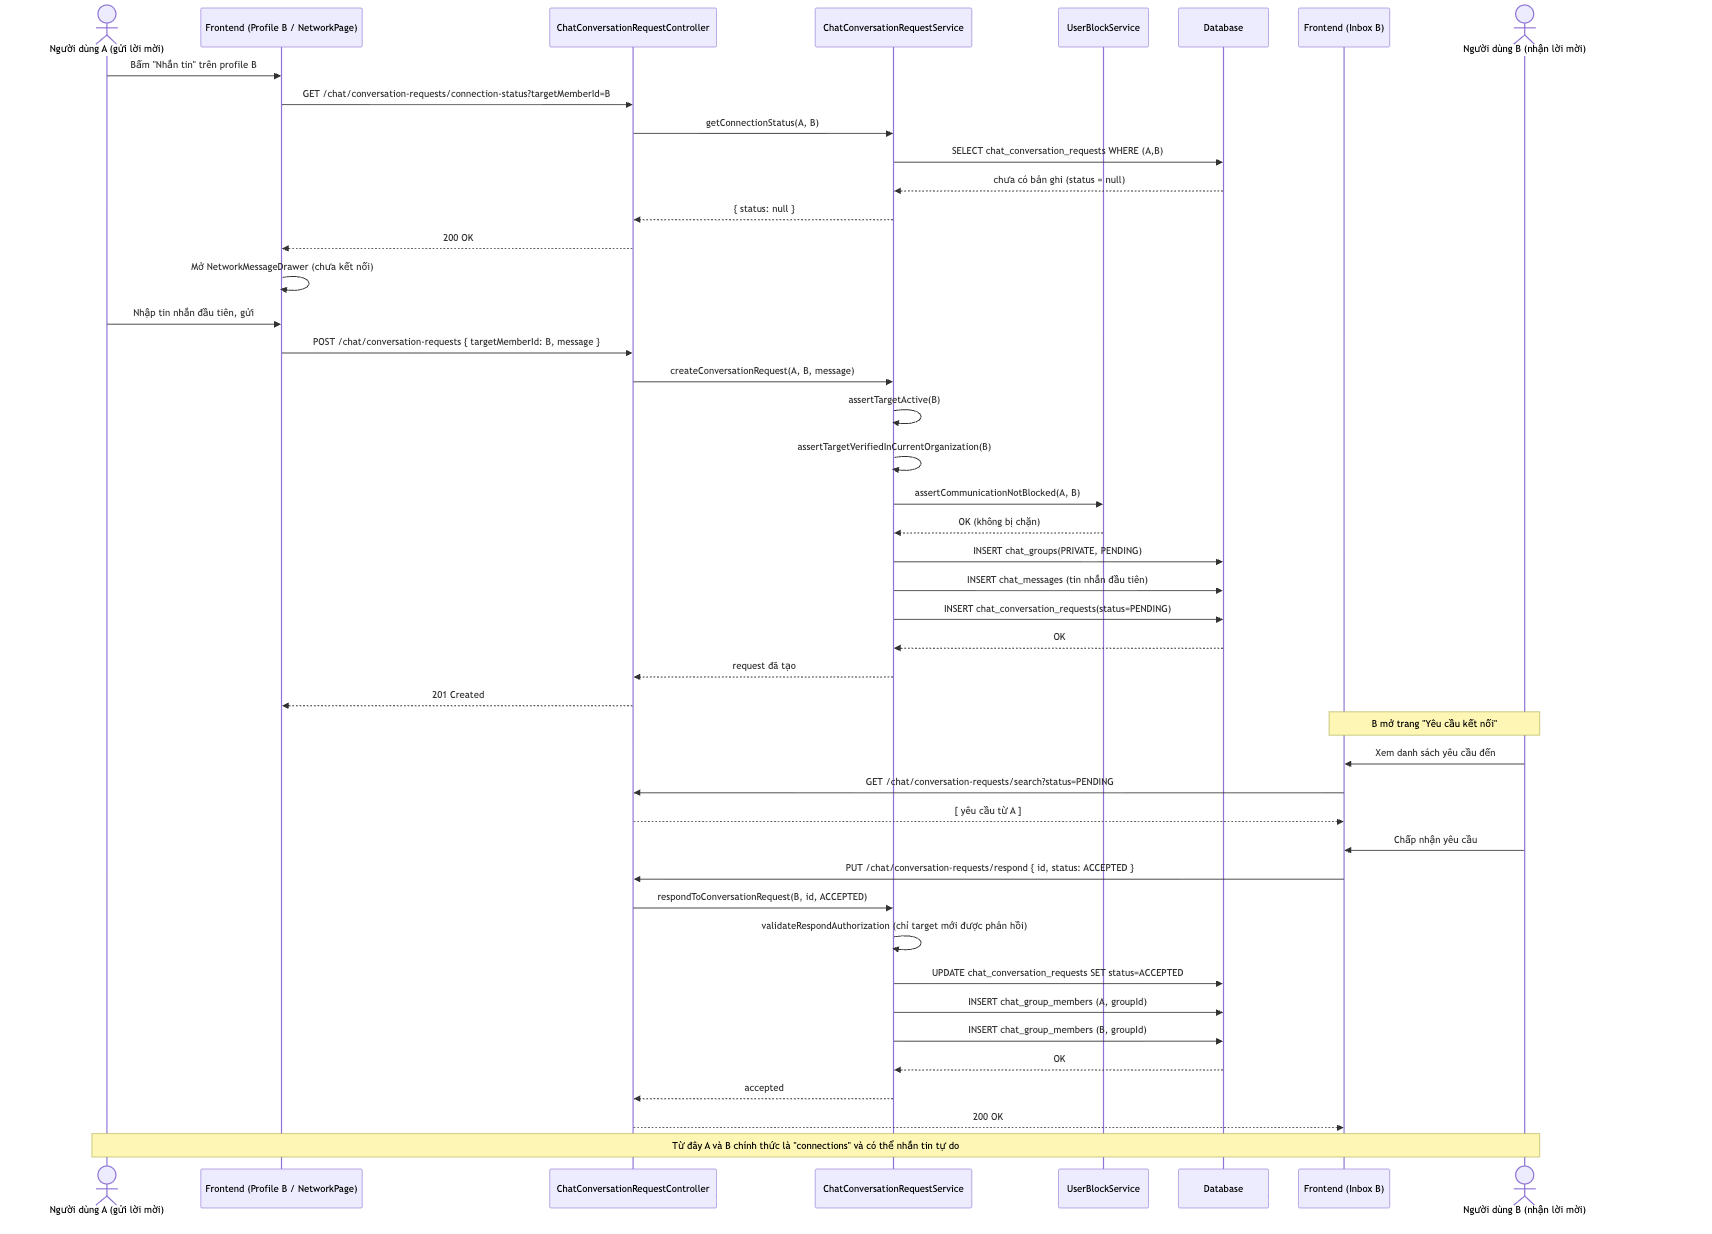
\includegraphics[width=1.0\textwidth,keepaspectratio]{sd-sequence-ketnoi}
\caption{Sơ đồ tuần tự luồng gửi và chấp nhận yêu cầu kết nối trước khi nhắn tin}
\label{fig:seqconnect}
\end{figure}

\subsection{Trợ lý ảo}

Trợ lý ảo được triển khai như một dịch vụ độc lập, tách khỏi backend chính, giao tiếp với giao diện qua một điểm cuối riêng. Dịch vụ này áp dụng kiến trúc kết hợp truy hồi và sinh đã trình bày ở mục 2.1.

Ở giai đoạn nạp dữ liệu, hệ thống đọc các tài liệu nguồn gồm nội dung giới thiệu nhà trường và tài liệu hướng dẫn sử dụng hệ thống, tách thành các đoạn văn bản có độ dài giới hạn kèm phần chồng lấn giữa các đoạn liền kề để không cắt đứt ngữ cảnh, chuyển mỗi đoạn thành vector biểu diễn ngữ nghĩa bằng một mô hình embedding đa ngữ có hỗ trợ tốt tiếng Việt, rồi lưu vào một chỉ mục vector. Hệ thống cho phép thêm và gỡ tài liệu ngay khi đang vận hành, nên tri thức của trợ lý ảo được cập nhật mà không cần huấn luyện lại mô hình.

Ở giai đoạn trả lời, câu hỏi của người dùng được chuyển thành vector theo cùng mô hình embedding, hệ thống truy hồi những đoạn có độ tương đồng cao nhất, có thể qua thêm một bước sắp xếp lại theo mức độ liên quan, rồi đưa các đoạn này vào ngữ cảnh của lời nhắc.

Lời nhắc được thiết kế theo hướng ràng buộc chặt nhằm chống bịa đặt thông tin. Mô hình được yêu cầu chỉ trả lời dựa trên ngữ cảnh đã truy hồi, luôn trả lời bằng tiếng Việt, từ chối các câu hỏi nằm ngoài phạm vi giới thiệu trường, thông tin khoa ngành và hướng dẫn sử dụng, đồng thời từ chối trả lời khi ngữ cảnh không đủ thông tin thay vì suy đoán. Mô hình cũng được yêu cầu dẫn tên tài liệu nguồn khi cần.

Câu trả lời được truyền về giao diện theo cơ chế đẩy dữ liệu một chiều, cho phép hiển thị dần từng phần thay vì chờ toàn bộ câu trả lời hoàn tất, cải thiện rõ rệt cảm nhận về tốc độ phản hồi.

\begin{figure}[H]\centering
\begin{tikzpicture}[font=\footnotesize,node distance=5mm,
 b/.style={draw,rounded corners=2pt,align=center,inner sep=3pt,minimum height=7mm,text width=24mm},
 ing/.style={b,fill=orange!10}, qry/.style={b,fill=blue!8},
 ar/.style={-{Latex[length=2mm]},thick}]
\node[ing] (doc) {Tài liệu nguồn\\ \scriptsize(giới thiệu trường, hướng dẫn)};
\node[ing,right=of doc] (split) {Tách đoạn\\ \scriptsize(1500 ký tự, chồng lấn 300)};
\node[ing,right=of split] (emb) {Mô hình embedding\\ \scriptsize đa ngữ};
\node[ing,right=of emb] (idx) {Chỉ mục vector\\ FAISS};
\begin{scope}[on background layer]
\node[draw,dashed,rounded corners,fill=orange!3,fit={(doc)(idx)},inner sep=3mm,
 label={[font=\scriptsize\bfseries]above:Giai đoạn nạp dữ liệu (thêm, gỡ tài liệu khi đang vận hành)}] {};
\end{scope}
\node[qry,below=16mm of doc] (q) {Câu hỏi\\ người dùng};
\node[qry,right=of q] (qe) {Mã hóa câu hỏi\\ \scriptsize cùng mô hình embedding};
\node[qry,right=of qe] (ret) {Truy hồi top-k\\ \scriptsize và sắp xếp lại};
\node[qry,right=of ret] (llm) {Lời nhắc ràng buộc\\ + mô hình ngôn ngữ};
\node[qry,below=9mm of llm,fill=green!10] (sse) {Trả lời theo dòng\\ về giao diện};
\begin{scope}[on background layer]
\node[draw,dashed,rounded corners,fill=blue!3,fit={(q)(llm)},inner sep=3mm,
 label={[font=\scriptsize\bfseries]below left:Giai đoạn trả lời}] {};
\end{scope}
\draw[ar] (doc)--(split); \draw[ar] (split)--(emb); \draw[ar] (emb)--(idx);
\draw[ar] (q)--(qe); \draw[ar] (qe)--(ret); \draw[ar] (ret)--(llm); \draw[ar] (llm)--(sse);
\draw[ar,dashed] (idx.south) -- node[fill=white,inner sep=1pt,font=\scriptsize,pos=0.55]{tra cứu} (ret.north);
\end{tikzpicture}
\caption{Kiến trúc trợ lý ảo theo mô hình kết hợp truy hồi và sinh}
\label{fig:ragarch}
\end{figure}

\subsection{Các tác vụ ứng dụng mô hình ngôn ngữ khác}

Ngoài trợ lý ảo, backend chính còn tích hợp mô hình ngôn ngữ cho một số tác vụ có đầu ra cấu trúc, không cần truy hồi tài liệu. Các tác vụ này gồm trích xuất thẻ kỹ năng từ mô tả chuyên môn của người cố vấn, trích xuất thông tin từ hồ sơ năng lực, nhận dạng ký tự quang học trên giấy tờ xác minh kèm bước làm sạch kết quả, kiểm duyệt nội dung do người dùng đăng, và tự động gắn thẻ chủ đề cho bài viết trên diễn đàn.

Hệ thống quản lý các nhà cung cấp và mô hình thông qua một sổ đăng ký cho phép quản trị viên lựa chọn mô hình sử dụng, kèm cơ chế dự phòng tự động chuyển sang mô hình khác khi mô hình đang dùng không phản hồi. Cơ chế này quan trọng vì các dịch vụ mô hình ngôn ngữ đều có giới hạn tần suất gọi và có thể tạm thời không sẵn sàng.

\subsection{Các phân hệ nghiệp vụ còn lại}

Phân hệ quản lý người dùng phụ trách hồ sơ cá nhân, học vấn, quá trình công tác và kỹ năng, kèm quy trình xác minh danh tính cho phép người dùng che bớt thông tin nhạy cảm trên giấy tờ. Hệ thống hỗ trợ thêm hình thức xác minh chéo, trong đó cựu sinh viên đã được xác minh có thể bảo lãnh cho người quen, giúp giảm tải cho quản trị viên.

Phân hệ quản lý tổ chức phụ trách khởi tạo đơn vị, cấu hình bộ nhận diện, bật tắt tính năng, cấp tài khoản quản trị theo phạm vi và gán đường dẫn riêng cho từng đơn vị.

Phân hệ nội dung quản lý tin tức, bài viết cựu sinh viên tiêu biểu, thành tích, tin tuyển dụng và học liệu theo một mô hình chung gồm soạn thảo, gửi duyệt, xuất bản và tìm kiếm. Người dùng có thể lưu lại nội dung quan tâm để xem sau.

Phân hệ sự kiện phụ trách vòng đời sự kiện từ khởi tạo, xuất bản, tiếp nhận đăng ký, phát hành vé điện tử có mã sinh theo token, đến điểm danh bằng mã QR trên cả web và di động, và cuối cùng là tổng hợp thống kê tham dự kèm xuất tệp báo cáo.

Phân hệ diễn đàn tổ chức nội dung theo cây chuyên mục thay vì dòng thời gian tự do, hỗ trợ tạo chủ đề, trả lời, bày tỏ cảm xúc, theo dõi chủ đề và các thao tác kiểm duyệt như khóa, ghim, ẩn bài. Tính toàn vẹn dữ liệu giữa các đơn vị luôn được kiểm tra qua định danh tổ chức trước mọi thao tác ghi.

Phân hệ khảo sát cho phép quản trị soạn biểu mẫu, phát tới nhóm người dùng mục tiêu, thu thập phản hồi và tổng hợp kết quả, phục vụ trực tiếp nghĩa vụ báo cáo tình hình việc làm của sinh viên tốt nghiệp.

Phân hệ thông báo tổng hợp thông báo trong ứng dụng theo loại và trạng thái đã đọc, kết hợp đẩy thông báo tới thiết bị di động và cập nhật giao diện tức thời qua kênh sự kiện một chiều.

\section{Tối ưu hiệu năng và trải nghiệm}

\subsection{Chiến lược lưu đệm nhiều tầng}

Hệ thống áp dụng chiến lược lưu đệm ở ba tầng khác nhau.

Ở tầng backend, dự án không sử dụng bộ nhớ đệm phân tán mà áp dụng cơ chế lưu đệm trong tiến trình. Toàn bộ việc lưu đệm được triển khai thủ công thông qua một lớp tiện ích dùng chung quản lý nhiều vùng đệm độc lập, mỗi vùng có tên và thời gian sống riêng, theo mô hình đọc trước và tính sau khi không tìm thấy. Cơ chế này được áp dụng cho nhiều nghiệp vụ khác nhau như lưu mã dùng một lần tạm thời khi đăng ký hoặc đổi mật khẩu, lưu danh sách chuyên mục và trạng thái có bài mới của diễn đàn phục vụ tác vụ định kỳ gửi thông báo, lưu thông tin tổ chức, sự kiện sắp diễn ra, thống kê quỹ và các số liệu cho trang quản trị. Thời gian sống của mỗi vùng dao động từ một phút đến một ngày tùy mức độ thay đổi của dữ liệu. Ngoài ra, hệ thống dùng bộ nhớ đệm riêng cho hai mục đích bảo mật là lưu kết quả xác minh chữ ký token để tránh xác minh lại nhiều lần, và làm bộ đếm cho cơ chế giới hạn tần suất truy cập theo địa chỉ với các điểm cuối nhạy cảm.

Ở tầng giao diện web, dự án dùng thư viện đồng bộ dữ liệu làm tầng đệm cho dữ liệu lấy từ API, cấu hình thời gian dữ liệu còn được xem là mới và tắt cơ chế tự động tải lại khi cửa sổ được kích hoạt lại. Một số nơi có tần suất thay đổi khác biệt được cấu hình riêng, và bộ đệm được chủ động làm mới sau các thao tác tạo, sửa hoặc xóa.

Ở tầng hạ tầng, máy chủ web được cấu hình lưu đệm dài hạn cho hình ảnh tĩnh, giúp giảm băng thông cho các tài nguyên ít thay đổi. Trên ứng dụng di động, việc lưu đệm chủ yếu áp dụng cho hình ảnh.

\subsection{Tối ưu truy vấn và giao diện}

Ở tầng dữ liệu, các truy vấn được viết tường minh kèm chỉ mục phù hợp, trong đó định danh tổ chức luôn nằm ở vị trí đầu của chỉ mục ghép. Việc không dùng cơ chế nạp trì hoãn buộc nhóm phải chủ động thiết kế số lần truy vấn cho mỗi nghiệp vụ, qua đó tránh được vấn đề phát sinh truy vấn ngoài kiểm soát.

Ở tầng giao diện, việc tách bạch trạng thái giao diện và dữ liệu máy chủ cùng với cơ chế lưu đệm giúp giảm đáng kể số lần gọi lại backend. Kỹ thuật quản lý biểu mẫu không kiểm soát giúp giảm số lần vẽ lại khi người dùng nhập liệu.

\subsection{Giảm độ trễ bằng truy vấn song song}

Nhiều điểm cuối của hệ thống phải tổng hợp dữ liệu từ nhiều nguồn độc lập nhau trước khi trả về. Bảng điều khiển quản trị cần đồng thời số người dùng, số bài viết chờ duyệt, số sự kiện sắp diễn ra và tiến độ các chiến dịch gây quỹ; trang chi tiết một buổi cố vấn cần đồng thời hồ sơ người cố vấn, danh sách chuyên môn và bản ghi phản hồi. Nếu thực hiện tuần tự, tổng độ trễ bằng tổng độ trễ của từng truy vấn.

Vì các truy vấn này không phụ thuộc kết quả của nhau, hệ thống áp dụng mô hình phân tán rồi gom kết quả: các truy vấn được phát đi cùng lúc và chỉ chờ tại điểm gộp, nhờ toán tử gộp nhiều luồng phản ứng của thư viện Reactor. Khi đó tổng độ trễ tiệm cận độ trễ của truy vấn chậm nhất thay vì tổng của tất cả. Đây là kỹ thuật được dùng lặp lại ở khoảng sáu mươi vị trí trong mã nguồn, tập trung ở các dịch vụ quản trị và các điểm cuối tổng hợp. Điểm đáng chú ý là kỹ thuật này chỉ phát huy tác dụng trên nền không chặn luồng: với mô hình cấp một luồng cho mỗi yêu cầu, việc chạy song song bốn truy vấn đồng nghĩa với việc chiếm bốn luồng cho một yêu cầu.

\subsection{Giới hạn tần suất và tối ưu chuyển đổi dữ liệu}

Hệ thống đặt một bộ lọc giới hạn tần suất ở lớp ngoài cùng của chuỗi xử lý, hoạt động theo thuật toán thùng token với ba hạn mức phân biệt theo tính chất điểm cuối: năm yêu cầu mỗi phút cho nhóm điểm cuối xác thực, năm yêu cầu mỗi phút cho nhóm tải tệp lên, và một trăm yêu cầu mỗi phút cho các điểm cuối còn lại. Việc tách riêng hạn mức cho nhóm xác thực nhằm chặn dò mật khẩu tự động, còn hạn mức cho nhóm tải tệp nhằm tránh một người dùng chiếm hết băng thông và dung lượng lưu trữ. Trạng thái thùng token được giữ trong bộ nhớ đệm trong tiến trình theo khóa gồm địa chỉ mạng và nhóm hạn mức, giới hạn hai mươi nghìn mục và tự thu hồi sau mười phút không truy cập, nên cơ chế này không cần thêm hạ tầng lưu trữ ngoài. Các đường dẫn phục vụ tài liệu API và điểm cuối giám sát được loại trừ khỏi bộ lọc để không cản trở việc vận hành.

Ở tầng chuyển đổi dữ liệu, hệ thống đăng ký một module tăng tốc cho bộ chuyển đổi JSON. Module này sinh mã truy cập thuộc tính ở dạng bytecode thay vì dùng cơ chế phản chiếu, giúp giảm chi phí đọc và ghi JSON. Với một hệ thống mà phần lớn thời gian xử lý nằm ở việc tuần tự hóa danh sách đối tượng trả về, khoản tiết kiệm này lặp lại trên mọi yêu cầu.

\subsection{Tối ưu trải nghiệm người dùng}

Hệ thống hỗ trợ chuyển đổi giữa giao diện sáng và tối, chuyển đổi giữa tiếng Việt và tiếng Anh, cùng cơ chế thông báo thời gian thực giúp người dùng nhận biết ngay khi có sự kiện liên quan mà không cần tải lại trang.

\section{Hạ tầng, vận hành và bảo mật ứng dụng}

Môi trường vận hành được định nghĩa bằng Docker Compose, gồm cơ sở dữ liệu, máy chủ ứng dụng, máy chủ web và hệ thống giám sát. Máy chủ web đóng vai trò trung gian chuyển tiếp yêu cầu tới backend và phục vụ nội dung tĩnh.

Hệ thống giám sát thu thập chỉ số vận hành và trực quan hóa qua bảng điều khiển, cho phép theo dõi tình trạng sức khỏe của ứng dụng theo thời gian. Chi tiết về các nhóm chỉ số được trình bày ở Chương 5.

Về bảo mật ứng dụng, hệ thống áp dụng nhiều biện pháp. Việc dùng truy vấn tham số hóa của tầng truy cập dữ liệu loại bỏ nguy cơ chèn mã vào câu truy vấn. Dữ liệu người dùng nhập được làm sạch ở phía giao diện nhằm giảm rủi ro chèn mã kịch bản. Token không lưu trạng thái phía máy chủ giúp hệ thống mở rộng dễ dàng. Công cụ kiểm tra người dùng thật được đặt ở màn hình đăng nhập và đăng ký. Cơ chế giới hạn tần suất truy cập bảo vệ các điểm cuối nhạy cảm như đăng nhập và tải tệp.

Hệ thống cũng ghi nhận lịch sử đăng nhập và đánh dấu các phiên có dấu hiệu bất thường để người dùng tự kiểm tra.

Một hạn chế còn tồn tại là việc phân quyền ở mức phương thức bằng chú thích chưa được áp dụng thống nhất; hiện việc kiểm tra quyền vẫn thực hiện trong thân phương thức nghiệp vụ. Nội dung này được ghi nhận ở phần hạn chế tại Chương 6.

% ─────────────────────── CHƯƠNG 5 ───────────────────────
\chapter{THỬ NGHIỆM VÀ ĐÁNH GIÁ}

Chương này trình bày chiến lược và môi trường kiểm thử, kết quả kiểm thử chức năng, đánh giá mức độ hoàn thành theo module, đánh giá hiệu năng, đối chiếu với hệ thống 2024, kiểm chứng cơ chế cô lập dữ liệu đa đơn vị, và thiết kế cùng giới hạn của quá trình thử nghiệm với người dùng.

\section{Chiến lược và môi trường kiểm thử}

\subsection{Các mức kiểm thử}

Nhóm áp dụng nhiều mức kiểm thử bổ trợ cho nhau.

Ở mức kiểm thử đơn vị, backend có 215 hàm kiểm thử cho tầng nghiệp vụ, chia thành 21 lớp kiểm thử, cùng một lớp kiểm tra khả năng nạp ngữ cảnh ứng dụng. Bộ kiểm thử sử dụng JUnit 5 làm khung chạy, Mockito để giả lập các phụ thuộc và một công cụ chuyên dụng để kiểm thử luồng phản ứng. Công cụ này cần thiết vì trong môi trường bất đồng bộ, kết quả của một lời gọi không trả về ngay mà phát ra theo thời gian, nên không thể kiểm tra bằng phép so sánh thông thường.

Ở mức kiểm thử tích hợp, nhóm kiểm tra sự phối hợp giữa các tầng và với cơ sở dữ liệu thật cho các luồng có nhiều thao tác ghi liên quan như đăng ký kèm kích hoạt, đặt lịch cố vấn và ghi nhận đóng góp quỹ. Cần nói rõ rằng mức này hiện được thực hiện thủ công trên môi trường dựng bằng Docker Compose chứ chưa được tự động hóa thành lớp kiểm thử chạy cùng bộ kiểm thử đơn vị. Việc bổ sung kiểm thử tích hợp tự động là một hạng mục đã được nhận diện ở Chương 6.

Ở mức kiểm thử hệ thống, nhóm thực hiện kiểm thử hộp đen theo luồng người dùng cho từng tính năng trong danh mục, trên cả web và ứng dụng di động. Ứng dụng di động được kiểm thử trên cả trình giả lập và thiết bị thật.

Ở mức kiểm thử thủ công, các tích hợp đặc biệt không thể tự động hóa dễ dàng được kiểm tra bằng tay, gồm luồng gọi lại từ cổng thanh toán, kết nối thời gian thực và luồng trả lời theo dòng của trợ lý ảo.

Frontend hiện chưa có kiểm thử tự động. Đây là một hạn chế đã được nhận diện và trình bày ở Chương 6.

\subsection{Độ phủ mã nguồn của bộ kiểm thử đơn vị}

Độ phủ mã nguồn được đo bằng JaCoCo sau khi chạy toàn bộ bộ kiểm thử đơn vị. Kết quả được trình bày ở Bảng \ref{tab:coverage}.

\renewcommand{\arraystretch}{1.25}
{\small
\begin{longtable}{|>{\raggedright\arraybackslash}p{7.0cm}|c|}
\caption{Độ phủ mã nguồn đo bằng JaCoCo}\label{tab:coverage}\\
\hline \textbf{Chỉ số} & \textbf{Giá trị} \\ \hline
\endfirsthead
\multicolumn{2}{l}{\itshape\small (tiếp theo trang trước)}\\[2pt]
\hline \textbf{Chỉ số} & \textbf{Giá trị} \\ \hline
\endhead
\hline
\endlastfoot
Độ phủ lớp (Class Coverage) & 58\% \\ \hline
Độ phủ dòng lệnh (Line Coverage) & 19\% \\ \hline
Độ phủ chỉ thị (Instruction Coverage) & 17\% \\ \hline
Độ phủ phương thức (Method Coverage) & 17\% \\ \hline
Độ phủ nhánh (Branch Coverage) & 7\% \\ \hline
\end{longtable}
}
\renewcommand{\arraystretch}{1}

Con số này cần được diễn giải đúng thay vì né tránh. Độ phủ lớp đạt 58\% cho thấy bộ kiểm thử đã chạm tới quá nửa số lớp của hệ thống, nhưng độ phủ dòng lệnh 19\% và đặc biệt độ phủ nhánh 7\% cho thấy phần lớn nhánh rẽ chưa được kiểm thử tự động. Nguyên nhân trực tiếp là bộ kiểm thử đơn vị hiện tập trung vào tầng nghiệp vụ của một số phân hệ, trong khi tầng controller, tầng truy cập dữ liệu và nhiều nhánh xử lý lỗi vẫn dựa vào kiểm thử thủ công.

Đáng chú ý là hai cơ chế kỹ thuật trọng tâm của đề tài đều chưa có kiểm thử đơn vị cho đúng nhánh quyết định. Lớp kiểm thử của dịch vụ đối soát giao dịch hiện kiểm tra các trường hợp sai khóa xác thực, sai loại giao dịch và trường hợp xử lý thành công, nhưng chưa có ca kiểm thử cho nhánh bỏ qua khi bản ghi đã ở trạng thái thành công, tức là chính nhánh bảo đảm xử lý một lần. Tương tự, luồng đặt lịch cố vấn chưa có lớp kiểm thử đơn vị riêng. Đây là khoảng trống được nhóm chủ động ghi nhận, và hướng xử lý được trình bày ở Chương 6.

\subsection{Môi trường và công cụ kiểm thử}

Môi trường kiểm thử được dựng bằng Docker Compose, tái lập đầy đủ các thành phần của môi trường vận hành gồm cơ sở dữ liệu, máy chủ ứng dụng và máy chủ web, nhằm bảo đảm kết quả kiểm thử phản ánh đúng hành vi thực tế.

Các điểm cuối được kiểm thử qua tài liệu API tương tác và qua công cụ gửi yêu cầu chuyên dụng, trong đó nhóm sử dụng biến môi trường để chuyển đổi nhanh giữa môi trường cục bộ và môi trường triển khai, đồng thời gom các điểm cuối cùng mục đích thành từng bộ sưu tập.

Việc kiểm thử tải được thực hiện bằng một công cụ kiểm thử tải hiện đại cho phép mô tả kịch bản bằng mã, thuận tiện cho việc đưa vào quy trình tự động và tái lập kết quả.

\section{Kết quả kiểm thử chức năng}

Nhóm xây dựng bộ test case chức năng bám theo luồng người dùng. Danh mục được tài liệu hóa đầy đủ gồm 15 test case, phân bố theo phân hệ như ở Bảng \ref{tab:testcases}. Đặc tả chi tiết từng test case được trình bày ở Phụ lục B.

\renewcommand{\arraystretch}{1.25}
{\small
\begin{longtable}{|c|>{\raggedright\arraybackslash}p{5.4cm}|>{\raggedright\arraybackslash}p{4.6cm}|c|}
\caption{Phân bố test case chức năng theo phân hệ}\label{tab:testcases}\\
\hline \textbf{STT} & \textbf{Phân hệ} & \textbf{Mã test case} & \textbf{Số lượng} \\ \hline
\endfirsthead
\multicolumn{4}{l}{\itshape\small (tiếp theo trang trước)}\\[2pt]
\hline \textbf{STT} & \textbf{Phân hệ} & \textbf{Mã test case} & \textbf{Số lượng} \\ \hline
\endhead
\hline \multicolumn{4}{r}{\itshape\small (còn tiếp)}\\
\endfoot
\hline
\endlastfoot
1 & Nội dung và kiểm duyệt & TC-ARTICLE-01 đến 04 & 4 \\ \hline
2 & Xác thực và tài khoản & TC-AUTH-01 đến 03 & 3 \\ \hline
3 & Sự kiện và vé điện tử & TC-EVENT-01, TC-EVENT-02 & 2 \\ \hline
4 & Giao diện đáp ứng và chủ đề & TC-UI-01, TC-UI-02 & 2 \\ \hline
5 & Gây quỹ & TC-DONATION-01 & 1 \\ \hline
6 & Nhắn tin & TC-CHAT-01 & 1 \\ \hline
7 & Phân quyền quản trị & TC-ADMIN-01 & 1 \\ \hline
8 & Ứng dụng di động & TC-MOBILE-01 & 1 \\ \hline
\multicolumn{3}{|r|}{\textbf{Tổng cộng}} & \textbf{15} \\ \hline
\end{longtable}
}
\renewcommand{\arraystretch}{1}

Phân bố test case tập trung ở nhóm nội dung, xác thực và sự kiện, là các luồng có nhiều bước và nhiều trạng thái trung gian nhất khi thao tác trên giao diện. Cần nêu rõ một khoảng trống: danh mục này chưa có test case được tài liệu hóa cho phân hệ cố vấn, dù đây là nhóm tính năng trọng tâm về mặt giá trị của đề tài. Việc kiểm tra phân hệ cố vấn hiện vẫn được thực hiện theo luồng người dùng nhưng chưa được ghi lại thành đặc tả có mã số, và đây là hạng mục cần bổ sung trước khi hệ thống được vận hành chính thức.

Toàn bộ 15 test case đều cho kết quả đạt. Dưới đây là bốn test case tiêu biểu được trình bày đầy đủ nhằm minh họa cách nhóm đặc tả và ghi nhận kết quả.

\renewcommand{\arraystretch}{1.25}
{\small
\begin{longtable}{|>{\raggedright\arraybackslash}p{2.3cm}|>{\raggedright\arraybackslash}p{3.0cm}|>{\raggedright\arraybackslash}p{4.2cm}|>{\raggedright\arraybackslash}p{4.4cm}|}
\caption{Một số test case chức năng tiêu biểu}\label{tab:sampletc}\\
\hline \textbf{Mã} & \textbf{Tiền điều kiện} & \textbf{Các bước thực hiện} & \textbf{Kết quả mong đợi} \\ \hline
\endfirsthead
\multicolumn{4}{l}{\itshape\small (tiếp theo trang trước)}\\[2pt]
\hline \textbf{Mã} & \textbf{Tiền điều kiện} & \textbf{Các bước thực hiện} & \textbf{Kết quả mong đợi} \\ \hline
\endhead
\hline \multicolumn{4}{r}{\itshape\small (còn tiếp)}\\
\endfoot
\hline
\endlastfoot
TC-AUTH-02 & Tài khoản đã kích hoạt & Đăng nhập với mật khẩu sai & Hiển thị lỗi xác thực, không tạo phiên và không cấp token \\ \hline
TC-ARTICLE-04 & Người dùng chưa đủ mức xác minh & Truy cập tuyến đăng bài & Bị chuyển sang trang không đủ quyền hoặc bị khóa thao tác \\ \hline
TC-EVENT-02 & Tài khoản giáo vụ có quyền điểm danh & Quét mã QR của một vé hợp lệ & Vé được điểm danh, trạng thái vé cập nhật đúng và không điểm danh được lần hai \\ \hline
TC-ADMIN-01 & Người dùng thường đã đăng nhập & Truy cập tuyến quản trị & Không truy cập được trang quản trị, hệ thống chặn ở cả tầng giao diện và tầng điểm cuối \\ \hline
\end{longtable}
}
\renewcommand{\arraystretch}{1}

Bốn test case trên cho thấy cách nhóm đặc tả điều kiện đầu vào, các bước thao tác và tiêu chí chấp nhận, trong đó TC-ARTICLE-04 và TC-ADMIN-01 kiểm chứng trực tiếp nguyên tắc chặn phân quyền ở cả hai tầng đã trình bày ở mục 3.2.2. Ngược lại, hai cơ chế kỹ thuật trọng tâm là kiểm soát trùng lịch khi đặt lịch cố vấn và bảo đảm xử lý một lần khi đối soát giao dịch hiện chưa có test case chức năng được tài liệu hóa, cũng chưa có kiểm thử đơn vị cho đúng nhánh quyết định như đã nêu ở mục 5.1.3. Việc bổ sung hai ca kiểm thử này là hạng mục ưu tiên và được trình bày ở Chương 6.

\section{Đánh giá mức độ hoàn thành}

\subsection{Mức độ hoàn thành theo module}

Danh mục tính năng sau rà soát gồm 86 tính năng thuộc 15 module. Tính đến thời điểm viết báo cáo, 80 tính năng đã hoàn thiện và 6 tính năng đang trong quá trình hoàn thiện.

Về phương pháp đánh giá, báo cáo không sử dụng tỉ lệ phần trăm hoàn thành cho từng tính năng, vì con số dạng này khó có căn cứ khách quan và dễ gây tranh cãi khi bảo vệ. Thay vào đó, mỗi tính năng được ghi nhận ở dạng phân loại trạng thái, và tỉ lệ hoàn thành của hệ thống được tính bằng số tính năng đã hoàn thiện chia cho tổng số tính năng thuộc phạm vi. Một tính năng được xem là hoàn thiện khi đã vận hành được trên đúng những nền tảng đã đặc tả cho tính năng đó, chứ không bị đánh giá thấp vì thiếu một nền tảng vốn không nằm trong phạm vi của nó. Theo cách tính này, hệ thống đạt tỉ lệ hoàn thành 93\%.

Sáu tính năng còn đang hoàn thiện gồm đính kèm phương tiện trong hội thoại, thông báo đẩy trên thiết bị di động, giao diện đa ngôn ngữ, trợ lý ảo hỏi đáp, quản trị kho tri thức của trợ lý ảo, và gợi ý quyết định duyệt bằng mô hình ngôn ngữ. Phần còn lại vì vậy tập trung ở nhóm tính năng ứng dụng trí tuệ nhân tạo và hoàn thiện trải nghiệm, không thuộc nhóm nghiệp vụ cốt lõi.

\renewcommand{\arraystretch}{1.2}
\begin{longtable}{|c|>{\raggedright\arraybackslash}p{6.6cm}|c|c|c|}
\caption{Mức độ hoàn thành theo module}\label{tab:completion}\\
\hline \textbf{STT} & \textbf{Module} & \textbf{Số tính năng} & \textbf{Hoàn thành} & \textbf{Đang làm} \\ \hline
\endfirsthead
\hline \textbf{STT} & \textbf{Module} & \textbf{Số tính năng} & \textbf{Hoàn thành} & \textbf{Đang làm} \\ \hline
\endhead
1 & Xác thực và phân quyền & 12 & 12 & 0 \\ \hline
2 & Hồ sơ người dùng & 3 & 3 & 0 \\ \hline
3 & Nội dung: tin tức, việc làm, học liệu, vinh danh & 8 & 8 & 0 \\ \hline
4 & Sự kiện & 7 & 7 & 0 \\ \hline
5 & Nhắn tin và mạng lưới kết nối & 8 & 7 & 1 \\ \hline
6 & Diễn đàn & 7 & 7 & 0 \\ \hline
7 & Thông báo & 3 & 2 & 1 \\ \hline
8 & Giao diện và trang công khai & 4 & 3 & 1 \\ \hline
9 & Tổ chức và đa đơn vị & 8 & 8 & 0 \\ \hline
10 & Cố vấn & 10 & 10 & 0 \\ \hline
11 & Gây quỹ & 5 & 5 & 0 \\ \hline
12 & Khảo sát & 2 & 2 & 0 \\ \hline
13 & Trợ lý ảo và ứng dụng AI & 4 & 1 & 3 \\ \hline
14 & Nền tảng dùng chung & 3 & 3 & 0 \\ \hline
15 & Ứng dụng di động & 2 & 2 & 0 \\ \hline
\multicolumn{2}{|r|}{\textbf{Tổng cộng}} & \textbf{86} & \textbf{80} & \textbf{6} \\ \hline
\end{longtable}
\renewcommand{\arraystretch}{1}

Nhìn chung, phần lớn module đạt mức hoàn thiện cao ở backend và web. Module trợ lý ảo có mức hoàn thiện thấp nhất ở phía backend do phần tích hợp giữa dịch vụ trợ lý ảo và hệ thống chính vẫn đang hoàn thiện. Các nền tảng di động có mức hoàn thiện thấp hơn web ở một số module do nhóm ưu tiên các luồng nghiệp vụ thường dùng khi di chuyển.

Cần lưu ý rằng các con số hoàn thành được hiểu theo phạm vi tính năng đã đặc tả, không phải mức độ phủ của kiểm thử tự động.

\subsection{Đối chiếu với mục tiêu và yêu cầu đã đặt ra}

Đối chiếu với năm mục tiêu nêu ở Chương 1, đề tài đạt được kết quả như sau.

Mục tiêu khảo sát nhu cầu và phân tích hiện trạng đã hoàn thành, với 90 phản hồi khảo sát và một bản phân tích chi tiết hệ thống 2024 làm căn cứ cho toàn bộ các quyết định thiết kế về sau.

Mục tiêu nghiên cứu và lựa chọn kiến trúc đã hoàn thành, thể hiện qua việc chuyển đổi thành công sang kiến trúc Modular Monolith kết hợp Layered trên nền phản ứng, kèm hỗ trợ đa đơn vị.

Mục tiêu phân tích, thiết kế và triển khai theo nhóm nghiệp vụ đã hoàn thành phần lớn, với 80 trên 86 tính năng hoàn thiện và toàn bộ 15 module đều có phần đã vận hành được.

Mục tiêu phát triển đồng thời web và di động dùng chung một tầng API đã hoàn thành, tuy mức độ phủ tính năng trên di động còn thấp hơn web.

Mục tiêu kiểm chứng hiệu quả của kiến trúc mới đã hoàn thành một phần. Cơ chế cô lập dữ liệu đã được kiểm chứng, nhưng số liệu đo hiệu năng dưới tải cần được bổ sung để hoàn tất mục tiêu này.

Đối chiếu với các yêu cầu phi chức năng nêu ở mục 3.1, hệ thống đáp ứng yêu cầu về mô hình xử lý bất đồng bộ, hỗ trợ đa đơn vị, và các cơ chế bảo mật cơ bản. Yêu cầu về khả năng bảo trì được đáp ứng ở tầng nghiệp vụ nhưng chưa trọn vẹn ở tầng giao diện do chưa có kiểm thử tự động.

Phần dưới đây đối chiếu trực tiếp từng nhu cầu đã khảo sát ở Chương 2 với phân hệ đã hiện thực, nhằm trả lời câu hỏi các module mới có thực sự chạm đúng vấn đề hay không.

Nhu cầu được xếp hạng cao nhất trong khảo sát là cơ hội nghề nghiệp, đạt 4,38 trên thang 5. Nhu cầu này được đáp ứng bằng ba phân hệ bổ trợ nhau chứ không phải một tính năng đơn lẻ: cổng việc làm cho phép cựu sinh viên và doanh nghiệp đăng tin trực tiếp tới đúng nhóm sinh viên của khoa, diễn đàn nghề nghiệp giữ lại các trao đổi về quy trình phỏng vấn và định hướng dưới dạng nội dung tra cứu được thay vì trôi mất như trên mạng xã hội, và chương trình cố vấn biến quan hệ nghề nghiệp từ trao đổi ngẫu nhiên thành buổi làm việc có lịch và có phản hồi. Đây chính là điểm khác biệt so với phiên bản 2024, vốn không có nhóm bảng dữ liệu nào cho việc làm và cố vấn có cấu trúc.

Nhu cầu tìm người cố vấn đạt 4,27 và là nhu cầu có khoảng cách lớn nhất giữa mong muốn và thực tế, vì trước đây việc kết nối phụ thuộc hoàn toàn vào quan hệ cá nhân. Phân hệ cố vấn giải quyết bằng cách chuẩn hóa toàn bộ vòng đời: cựu sinh viên khai báo hồ sơ chuyên môn và khung giờ rảnh, hệ thống gợi ý theo kỹ năng, người được cố vấn đặt lịch trong khung giờ còn trống, và mỗi buổi đều có trạng thái cùng phản hồi sau buổi. Nhờ vậy, việc cố vấn không còn phụ thuộc vào việc hai bên có quen nhau từ trước.

Nhu cầu về quỹ và học bổng đạt 3,98, thấp hơn nhóm nghề nghiệp nhưng lại là nhu cầu của phía nhà trường nhiều hơn phía người dùng. Phân hệ gây quỹ đáp ứng bằng chiến dịch có mục tiêu, tiến độ công khai và đặc biệt là cơ chế đối soát tự động, giúp bộ phận vận hành không phải rà soát sao kê thủ công. Đây là điểm mà một nền tảng thuần mạng xã hội không thể cung cấp.

Ở phía quản trị, nhu cầu lớn nhất là giảm chi phí vận hành khi mỗi khoa phải tự duy trì một hệ thống riêng. Kiến trúc đa đơn vị đáp ứng trực tiếp nhu cầu này: một lần triển khai phục vụ nhiều khoa, mỗi khoa giữ được bộ nhận diện và quyền tự quyết về nhóm tính năng bật tắt, trong khi dữ liệu vẫn tách biệt theo ba lớp bảo vệ đã kiểm chứng ở mục 5.5.

Hai nhu cầu chưa được đáp ứng trọn vẹn cần được nêu thẳng. Thứ nhất, trợ lý ảo thông tin đạt 3,84 trong khảo sát nhưng hiện mới trả lời trong phạm vi tài liệu đã nạp, chưa bao phủ các câu hỏi về dữ liệu cá nhân của người dùng như lịch cố vấn hay vé sự kiện của chính họ. Thứ hai, nhóm tính năng đa ngôn ngữ và thông báo đẩy trên di động vẫn nằm trong số sáu tính năng đang hoàn thiện, nên trải nghiệm trên di động chưa đồng đều với trải nghiệm trên web.

\section{Đánh giá hiệu năng và tính ổn định}

\subsection{Môi trường và công cụ đo}

Hệ thống được trang bị sẵn cơ chế đo lường ở mức ứng dụng, tự động ghi nhận thời gian xử lý của mọi yêu cầu và tính các phân vị thay vì chỉ lấy giá trị trung bình. Đây là điểm quan trọng về phương pháp: giá trị trung bình che giấu các yêu cầu chậm bất thường, trong khi phân vị thứ 95 và thứ 99 phản ánh đúng trải nghiệm của nhóm người dùng chịu độ trễ cao nhất.

Dữ liệu đo được thu thập vào hệ thống giám sát và trực quan hóa trên bảng điều khiển quản trị, cho phép lọc theo khoảng thời gian tùy chọn.

Việc tạo tải được thực hiện bằng công cụ kiểm thử tải mô tả kịch bản bằng mã. Ngoài ra, trong giai đoạn phát triển, nhóm dùng thêm công cụ giám sát máy ảo Java để quan sát mức tiêu thụ bộ nhớ và số luồng của tiến trình backend.

\subsection{Các nhóm chỉ số giám sát}

Hệ thống theo dõi bốn nhóm chỉ số.

Nhóm chỉ số về lưu lượng và độ trễ gồm tốc độ yêu cầu, tỉ lệ lỗi, độ trễ trung bình và các phân vị, cùng thống kê chi tiết cho các điểm cuối chịu tải cao nhất.

Nhóm chỉ số về hệ thống và máy ảo Java gồm mức sử dụng bộ xử lý, mức tiêu thụ bộ nhớ, hiệu suất thu gom rác, trạng thái nhóm kết nối cơ sở dữ liệu, số luồng và số mô tả tệp đang mở. Nhóm chỉ số này quan trọng vì trạng thái bão hòa của nhóm kết nối thường là dấu hiệu sớm nhất của nghẽn hệ thống.

Nhóm chỉ số về các tác vụ tốn tài nguyên gồm thời gian gửi thư điện tử, thời gian nhận dạng ký tự quang học, thời gian tải tệp và dung lượng lưu trữ.

Nhóm chỉ số nghiệp vụ và thời gian thực gồm tần suất đăng nhập thành công và thất bại, số yêu cầu bị chặn bởi cơ chế giới hạn tần suất, số phiên kết nối thời gian thực đang hoạt động và tần suất đẩy sự kiện.

\subsection{Kết quả giám sát ở tải vận hành thực tế}

Trước khi trình bày kết quả kiểm thử tải, mục này báo cáo số liệu giám sát thu được từ một phiên vận hành thực tế của hệ thống trên môi trường triển khai. Phiên kéo dài 2 giờ 36 phút, ghi nhận 1.753 yêu cầu với độ trễ trung bình toàn phiên là 26,78 ms. Bảng \ref{tab:monitoring} trích mười mốc đo liên tiếp cách nhau 30 giây ở cuối phiên, là giai đoạn hệ thống chịu tải cao nhất trong phiên. Hai cột tỉ lệ lỗi HTTP và số ngoại lệ ứng dụng không được đưa vào bảng vì đều bằng không ở toàn bộ mười mốc đo.

\renewcommand{\arraystretch}{1.15}
{\small
\begin{longtable}{|>{\centering\arraybackslash}p{1.9cm}|>{\centering\arraybackslash}p{1.2cm}|>{\centering\arraybackslash}p{1.5cm}|>{\centering\arraybackslash}p{1.5cm}|>{\centering\arraybackslash}p{1.5cm}|>{\centering\arraybackslash}p{1.8cm}|>{\centering\arraybackslash}p{1.5cm}|>{\centering\arraybackslash}p{1.6cm}|}
\caption{Số liệu giám sát theo mốc thời gian ở cuối phiên vận hành}\label{tab:monitoring}\\
\hline \textbf{Thời điểm} & \textbf{req/s} & \textbf{TB} & \textbf{p50} & \textbf{p99} & \textbf{CPU hệ} & \textbf{CPU JVM} & \textbf{Heap} \\
 & & \textbf{(ms)} & \textbf{(ms)} & \textbf{(ms)} & \textbf{thống (\%)} & \textbf{(\%)} & \textbf{(MB)} \\ \hline
\endfirsthead
\multicolumn{8}{l}{\itshape\small (tiếp theo trang trước)}\\[2pt]
\hline \textbf{Thời điểm} & \textbf{req/s} & \textbf{TB} & \textbf{p50} & \textbf{p99} & \textbf{CPU hệ} & \textbf{CPU JVM} & \textbf{Heap} \\
 & & \textbf{(ms)} & \textbf{(ms)} & \textbf{(ms)} & \textbf{thống (\%)} & \textbf{(\%)} & \textbf{(MB)} \\ \hline
\endhead
\hline
\endlastfoot
15:45:30 & 0,44 & 29,94 & 21,97 & 195,80 & 7,11 & 1,15 & 161,28 \\ \hline
15:46:00 & 0,55 & 31,50 & 21,94 & 255,55 & 16,17 & 0,19 & 154,46 \\ \hline
15:46:30 & 0,55 & 31,50 & 21,94 & 255,55 & 15,46 & 0,19 & 178,46 \\ \hline
15:47:00 & 0,42 & 31,17 & 23,77 & 197,15 & 13,39 & 0,15 & 203,46 \\ \hline
15:47:30 & 0,40 & 31,29 & 23,53 & 198,49 & 9,54 & 0,20 & 228,46 \\ \hline
15:48:00 & 0,12 & 42,18 & 22,37 & 260,92 & 7,12 & 0,13 & 253,46 \\ \hline
15:48:30 & 0,12 & 42,18 & 22,37 & 260,92 & 4,97 & 0,17 & 278,46 \\ \hline
15:49:00 & 0,12 & 42,18 & 22,37 & 260,92 & 10,75 & 0,15 & 302,46 \\ \hline
15:49:30 & 0,12 & 42,18 & 22,37 & 260,92 & 11,46 & 0,20 & 328,46 \\ \hline
15:50:00 & 0,12 & 42,18 & 22,37 & 260,92 & 10,77 & 0,15 & 144,87 \\ \hline
\end{longtable}
}
\renewcommand{\arraystretch}{1}

\begin{figure}[H]\centering
\begin{tikzpicture}
\begin{axis}[width=0.95\textwidth,height=6.2cm,
 xtick={0,1,2,3,4,5,6,7,8,9},
 xticklabels={15:45:30,15:46:00,15:46:30,15:47:00,15:47:30,15:48:00,15:48:30,15:49:00,15:49:30,15:50:00},
 x tick label style={rotate=45,anchor=east,font=\scriptsize},
 ylabel={Độ trễ (ms)},ylabel style={font=\small},
 yticklabel style={font=\scriptsize},
 ymin=0,ymax=300,grid=major,grid style={dashed,gray!30},
 legend style={font=\scriptsize,at={(0.5,-0.42)},anchor=north,legend columns=3,draw=none}]
\addplot[thick,blue!70,mark=*,mark size=1.3pt] coordinates {(0,21.97)
(1,21.94)
(2,21.94)
(3,23.77)
(4,23.53)
(5,22.37)
(6,22.37)
(7,22.37)
(8,22.37)
(9,22.37)};
\addlegendentry{p50}
\addplot[thick,green!55!black,mark=square*,mark size=1.3pt] coordinates {(0,29.94)
(1,31.50)
(2,31.50)
(3,31.17)
(4,31.29)
(5,42.18)
(6,42.18)
(7,42.18)
(8,42.18)
(9,42.18)};
\addlegendentry{trung bình}
\addplot[thick,orange!85!black,mark=triangle*,mark size=1.6pt] coordinates {(0,195.80)
(1,255.55)
(2,255.55)
(3,197.15)
(4,198.49)
(5,260.92)
(6,260.92)
(7,260.92)
(8,260.92)
(9,260.92)};
\addlegendentry{p99}
\end{axis}
\end{tikzpicture}
\caption{Độ trễ trung bình, phân vị 50 và phân vị 99 theo thời gian}
\label{fig:latency}
\end{figure}

\begin{figure}[H]\centering
\begin{tikzpicture}
\begin{axis}[width=0.95\textwidth,height=5.4cm,
 xtick={0,1,2,3,4,5,6,7,8,9},
 xticklabels={15:45:30,15:46:00,15:46:30,15:47:00,15:47:30,15:48:00,15:48:30,15:49:00,15:49:30,15:50:00},
 x tick label style={rotate=45,anchor=east,font=\scriptsize},
 ylabel={Bộ nhớ Heap (MB)},ylabel style={font=\small},
 yticklabel style={font=\scriptsize},
 ymin=100,ymax=360,grid=major,grid style={dashed,gray!30}]
\addplot[thick,violet!75,mark=*,mark size=1.3pt] coordinates {(0,161.28)
(1,154.46)
(2,178.46)
(3,203.46)
(4,228.46)
(5,253.46)
(6,278.46)
(7,302.46)
(8,328.46)
(9,144.87)};
\end{axis}
\end{tikzpicture}
\caption{Diễn biến bộ nhớ Heap của máy ảo Java trong cùng khoảng thời gian}
\label{fig:heap}
\end{figure}

Ba nhận xét rút ra từ số liệu này.

Thứ nhất, độ trễ phân vị 50 giữ ổn định quanh 22 ms trong suốt giai đoạn đo, gần như không dao động khi tốc độ yêu cầu thay đổi từ 0,55 xuống 0,12 yêu cầu mỗi giây. Khoảng cách giữa phân vị 50 và phân vị 99 là đáng kể, từ 22 ms lên khoảng 260 ms. Khoảng cách này đúng như dự đoán về mặt phương pháp đã nêu ở mục 5.4.1: giá trị trung bình 42 ms che giấu nhóm yêu cầu chậm nhất, và chỉ có phân vị cao mới phản ánh trải nghiệm của nhóm người dùng chịu độ trễ lớn nhất. Các yêu cầu ở phân vị 99 chủ yếu là những điểm cuối tổng hợp nhiều nguồn dữ liệu và những lần gọi đầu tiên khi bộ nhớ đệm còn rỗng.

Thứ hai, bộ nhớ Heap tăng đều từ 154 MB lên 328 MB rồi rơi về 145 MB ở mốc cuối. Đây là dạng răng cưa đặc trưng của một chu kỳ thu gom rác diễn ra bình thường, không phải dấu hiệu rò rỉ bộ nhớ. Thời gian tạm dừng do thu gom rác trong toàn bộ giai đoạn đo nằm trong khoảng 0,20 đến 0,37 ms, tức là không đủ lớn để ảnh hưởng tới độ trễ quan sát được. Mức sử dụng bộ xử lý của tiến trình máy ảo Java dao động quanh 0,2 phần trăm, cho thấy hệ thống hoàn toàn không bị giới hạn bởi năng lực tính toán ở mức tải này.

Thứ ba, trong toàn bộ giai đoạn đo, số lỗi HTTP và số ngoại lệ ứng dụng đều bằng không. Xét trên cả phiên, hệ thống ghi nhận 283 phản hồi thuộc nhóm lỗi trên tổng số 1.753 yêu cầu. Con số này cần được đọc đúng bản chất: biểu đồ phân bố mã trạng thái cho thấy toàn bộ các phản hồi này thuộc nhóm 403 và 404, phát sinh từ chính các kịch bản kiểm thử phân quyền và kiểm thử truy cập tài nguyên không tồn tại, tức là hệ thống trả về đúng mã lỗi mà kịch bản mong đợi. Không có phản hồi nào thuộc nhóm 5xx trong toàn phiên, nghĩa là không có lỗi phía máy chủ.

Cần nêu rõ phạm vi của phép đo này. Đây là số liệu giám sát trong điều kiện sử dụng thực tế với tốc độ yêu cầu cao nhất chỉ đạt 0,56 yêu cầu mỗi giây, nên nó chứng minh được tính ổn định, tính đúng đắn của cơ chế đo lường và trạng thái lành mạnh của bộ nhớ, nhưng hoàn toàn không phải là kiểm thử tải và không dùng để kết luận về giới hạn chịu tải của hệ thống.

\subsection{Kết quả kiểm thử tải}

Khác với số liệu giám sát ở mục trên, kiểm thử tải chủ động tạo tải vượt mức sử dụng thông thường nhằm xác định ngưỡng chịu đựng của hệ thống. Kịch bản mô phỏng số người dùng đồng thời tăng dần, đo thời gian phản hồi ở các phân vị, số kết nối thời gian thực duy trì đồng thời và độ trễ của luồng trả lời theo dòng. Tại thời điểm hoàn thành báo cáo, nhóm chưa thực hiện được đợt đo này, nên bảng và biểu đồ dưới đây được giữ ở dạng khung chờ số liệu.

\phtabl{Bảng kết quả kiểm thử tải, gồm các cột: Mức tải, Số yêu cầu mỗi giây, Độ trễ phân vị 50, Độ trễ phân vị 95, Tỉ lệ lỗi.}{Kết quả kiểm thử tải theo các mức người dùng đồng thời}{tab:loadtest}

\phfigl{5.5cm}{Biểu đồ đường thể hiện thời gian phản hồi ở phân vị 50 và phân vị 95 theo số người dùng đồng thời.}{Thời gian phản hồi theo số người dùng đồng thời}{fig:loadchart}

\subsection{Đánh giá hiệu năng theo điểm cuối tiêu biểu}

Bên cạnh số liệu tổng hợp, nhóm đo riêng một số điểm cuối đại diện cho các dạng tải khác nhau, gồm đăng nhập là điểm cuối có chi phí tính toán băm mật khẩu, tải thông tin tổ chức là điểm cuối đọc nhiều và có thể hưởng lợi từ lưu đệm, tải lịch sử hội thoại là điểm cuối đọc lượng dữ liệu lớn có phân trang, và tải danh sách bài viết là điểm cuối có nhiều phép kết bảng.

\phtabl{Bảng đo hiệu năng theo điểm cuối tiêu biểu, gồm các cột: Điểm cuối, Đặc điểm tải, Độ trễ trung bình, Độ trễ phân vị 95.}{Hiệu năng của một số điểm cuối tiêu biểu}{tab:apiperf}

\subsection{So sánh trước và sau khi áp dụng các biện pháp tối ưu}

Đây là phép đo có giá trị chứng minh cao nhất cho luận điểm tái thiết kế của đề tài, vì nó cho thấy chính các quyết định tối ưu của nhóm tạo ra khác biệt đo được, độc lập với việc so sánh với hệ thống 2024.

Phép đo được thực hiện trên cùng một bản dựng và cùng một kịch bản tải, chỉ thay đổi cấu hình của từng biện pháp tối ưu. Cụ thể, nhóm đo lần lượt trong các điều kiện tắt và bật cơ chế lưu đệm trong tiến trình, không có và có chỉ mục trên các cột lọc chính, và thay đổi kích thước nhóm kết nối cơ sở dữ liệu.

\phtabl{Bảng so sánh hiệu năng trước và sau khi áp dụng từng biện pháp tối ưu, gồm các cột: Biện pháp, Thời gian phản hồi trước, Thời gian phản hồi sau, Thông lượng trước, Thông lượng sau, Mức sử dụng bộ xử lý, Mức sử dụng bộ nhớ.}{So sánh hiệu năng trước và sau khi áp dụng các biện pháp tối ưu}{tab:beforeafter}

Cần nêu rõ một giới hạn về phương pháp. Nhóm có thể đo được tác động của việc lưu đệm, đánh chỉ mục và điều chỉnh nhóm kết nối vì các biện pháp này có thể bật tắt trên cùng một bản dựng. Ngược lại, nhóm không thể đưa ra phép so sánh trực tiếp giữa mô hình phản ứng và mô hình đồng bộ, vì hệ thống không có một bản hiện thực đồng bộ song song để đối chứng. Với luận điểm về mô hình phản ứng, báo cáo chỉ trình bày bằng chứng gián tiếp là số kết nối đồng thời duy trì được và số luồng tiêu tốn ở mức tải cao, kèm lập luận đối chiếu với đặc điểm của mô hình cấp một luồng cho mỗi yêu cầu.

\section{Đối chiếu với hệ thống AlumVerse 2024}

Phiên bản 2026 được đối chiếu với bản 2024 trên hai phương diện kiến trúc và nghiệp vụ, dựa trên Bảng \ref{tab:compare2024} đã trình bày ở Chương 2.

Về kiến trúc, mô hình chín dịch vụ nhỏ được thay bằng một ứng dụng nguyên khối chia module, giúp loại bỏ hoàn toàn chi phí vận hành hệ phân tán gồm đăng ký dịch vụ, cổng định tuyến và giám sát nhiều tiến trình. Mô hình xử lý chuyển từ đồng bộ sang bất đồng bộ, và hệ thống chuyển từ phục vụ một đơn vị sang phục vụ nhiều đơn vị trên cùng một lần triển khai.

Về nghiệp vụ, tính năng tư vấn dạng bài đăng của bản 2024 được thay bằng chương trình cố vấn có cấu trúc với đầy đủ vòng đời từ hồ sơ, ghép cặp, đặt lịch đến đánh giá. Hệ thống bổ sung các nhóm tính năng hoàn toàn mới gồm gây quỹ có đối soát, cổng việc làm và học liệu, khảo sát và trợ lý ảo. Tính năng nhắn tin được mở rộng từ chỉ hỗ trợ một đối một sang hỗ trợ cả hội thoại nhóm.

Về chất lượng, bản 2024 chưa kịp triển khai kiểm thử tự động, trong khi bản 2026 có 215 hàm kiểm thử cho tầng nghiệp vụ cùng quy trình tích hợp liên tục.

Cần nhắc lại giới hạn đã nêu ở Chương 2: nhóm không tiếp nhận mã nguồn của phiên bản 2024 nên không thể dựng lại hệ thống cũ để đo trong cùng điều kiện. Mọi số liệu về bản 2024 đều được trích dẫn từ báo cáo của khóa trước. Vì vậy, phép so sánh ở mục này mang tính đối chiếu định tính về kiến trúc và phạm vi nghiệp vụ, không phải một phép so sánh hiệu năng có kiểm soát.

\section{Kiểm chứng cơ chế cô lập dữ liệu đa đơn vị}

Do cô lập dữ liệu là yêu cầu bảo mật quan trọng nhất của mô hình đa đơn vị, nhóm xây dựng một bộ kịch bản kiểm chứng riêng.

Bộ kịch bản gồm các trường hợp: người dùng thuộc đơn vị A đăng nhập và truy vấn danh sách tin tức, sự kiện, chủ đề diễn đàn và danh sách người cố vấn; tài khoản quản trị của đơn vị A cố gắng truy cập trang cấu hình của đơn vị B; tài khoản quản trị của đơn vị A gửi yêu cầu sửa dữ liệu kèm định danh tổ chức của đơn vị B trong phần thân yêu cầu; và người dùng thuộc nhiều đơn vị chuyển đổi qua lại giữa các đơn vị.

\renewcommand{\arraystretch}{1.2}
\begin{longtable}{|>{\raggedright\arraybackslash}p{1.6cm}|>{\raggedright\arraybackslash}p{5.6cm}|>{\raggedright\arraybackslash}p{4.4cm}|>{\raggedright\arraybackslash}p{2.6cm}|}
\caption{Kịch bản và kết quả kiểm chứng cô lập dữ liệu}\label{tab:isolation}\\
\hline \textbf{Mã} & \textbf{Kịch bản} & \textbf{Kết quả mong đợi} & \textbf{Kết quả} \\ \hline
\endfirsthead
\hline \textbf{Mã} & \textbf{Kịch bản} & \textbf{Kết quả mong đợi} & \textbf{Kết quả} \\ \hline
\endhead
KC-01 & Người dùng thuộc đơn vị A truy vấn tin tức, sự kiện, chủ đề diễn đàn & Chỉ trả về dữ liệu của đơn vị A & Đạt \\ \hline
KC-02 & Quản trị đơn vị A mở trang cấu hình của đơn vị B & Bị từ chối truy cập & Đạt \\ \hline
KC-03 & Quản trị đơn vị A gửi yêu cầu sửa dữ liệu kèm định danh của đơn vị B trong thân yêu cầu & Bỏ qua giá trị gửi lên, áp phạm vi từ token & Đạt \\ \hline
KC-04 & Người dùng thuộc nhiều đơn vị chuyển đổi qua lại & Dữ liệu hiển thị lọc lại theo đơn vị mới & Đạt \\ \hline
KC-05 & Khách vãng lai xem nội dung công khai của nhiều đơn vị & Xem được, đúng thiết kế tham quan chéo & Đạt \\ \hline
\end{longtable}
\renewcommand{\arraystretch}{1}

Kết quả cho thấy dữ liệu giữa các đơn vị được tách biệt đúng phạm vi. Đáng chú ý nhất là kịch bản gửi kèm định danh tổ chức giả mạo trong thân yêu cầu: hệ thống bỏ qua giá trị này và vẫn áp dụng phạm vi lấy từ token đã ký, đúng như thiết kế đã trình bày ở mục 3.2.

\section{Thử nghiệm với người dùng: thiết kế, phạm vi và giới hạn đánh giá}

Để đánh giá giá trị thực tế của hệ thống, nhóm thiết kế một đợt thử nghiệm với người dùng theo kịch bản, tập trung vào các luồng không phụ thuộc vào một sự kiện có thật đang diễn ra.

Kịch bản thử nghiệm gồm đăng ký tài khoản và kích hoạt, duyệt và tham gia thảo luận trên diễn đàn, tìm kiếm và đặt lịch với một người cố vấn, tra cứu tin tuyển dụng và học liệu, và thực hiện một khoản đóng góp ở chế độ thử. Dữ liệu thu thập gồm các chỉ số định lượng cơ bản như số tài khoản đăng ký thành công, số lịch hẹn cố vấn được tạo, mức độ sử dụng diễn đàn, cùng phản hồi định tính về mức độ dễ hiểu của giao diện và những điểm gây nhầm lẫn.

\phtabl{Bảng kết quả thử nghiệm theo kịch bản với nhóm người dùng, gồm các cột: Kịch bản, Số người thực hiện, Tỉ lệ hoàn thành, Ghi nhận định tính.}{Kết quả thử nghiệm theo kịch bản với nhóm người dùng}{tab:usertest}

Cần trình bày rõ ba giới hạn của quá trình đánh giá này, bởi đây là những giới hạn xuất phát từ đặc thù sản phẩm chứ không phải thiếu sót về thiết kế.

Thứ nhất, hệ thống chưa được phát hành rộng rãi cho toàn bộ người dùng thật, nên các chỉ số thu được phản ánh hành vi trong một đợt thử nghiệm có kiểm soát, không phải số liệu vận hành ở quy mô toàn trường.

Thứ hai, nhóm người tham gia thử nghiệm không bao gồm vai trò quản trị. Các luồng quản trị như kiểm duyệt nội dung, duyệt hồ sơ cố vấn hay vận hành chiến dịch gây quỹ vì vậy chưa được nghiệm thu từ góc nhìn của người dùng cuối thực thụ, mà mới chỉ được kiểm thử bởi chính nhóm phát triển.

Thứ ba, một số phân hệ về bản chất cần gắn với hoạt động thực tế mới đánh giá được trọn vẹn. Điển hình là phân hệ sự kiện: luồng phát hành vé và điểm danh chỉ bộc lộ hết vấn đề khi vận hành trong một sự kiện có thật với số lượng người tham dự đủ lớn, điều nằm ngoài khả năng tổ chức của nhóm trong khuôn khổ đề tài.

Những giới hạn này được ghi nhận một cách minh bạch và là căn cứ để đề xuất hướng phát triển ở chương tiếp theo.

% ─────────────────────── CHƯƠNG 6 ───────────────────────
\chapter{KẾT LUẬN}

\section{Kết quả đạt được}

Đề tài đã hoàn thành việc tái thiết kế và mở rộng hệ thống kết nối sinh viên và cựu sinh viên của Trường Đại học Khoa học Tự nhiên theo hai hướng song song đã đặt ra từ đầu.

Về mặt kỹ thuật, nhóm đã xây dựng lại toàn bộ hệ thống từ kiến trúc Microservices với chín dịch vụ sang kiến trúc Modular Monolith kết hợp Layered với mười ba module nghiệp vụ, vận hành trên nền tảng phản ứng không chặn luồng. Hệ thống được mở rộng thành nền tảng đa đơn vị, cho phép nhiều khoa dùng chung một lần triển khai với dữ liệu được cô lập bằng ba lớp bảo vệ chồng nhau.

Về mặt nghiệp vụ, hệ thống hiện thực 86 tính năng thuộc 15 module trên 45 controller với 364 điểm cuối, trong đó 80 tính năng đã hoàn thiện. Trọng tâm sản phẩm được dịch chuyển từ mô hình mạng xã hội sang các nhóm tính năng tạo giá trị thực gồm chương trình cố vấn có cấu trúc, cổng việc làm và học liệu, gây quỹ có đối soát tự động, diễn đàn nghề nghiệp, khảo sát phục vụ thống kê việc làm và trợ lý ảo.

Về mặt chất lượng, hệ thống có 215 hàm kiểm thử đơn vị cho tầng nghiệp vụ, 15 test case chức năng được tài liệu hóa, quy trình tích hợp và triển khai liên tục, cùng hệ thống giám sát vận hành. Cơ chế cô lập dữ liệu đa đơn vị đã được kiểm chứng qua bộ kịch bản riêng.

Sản phẩm được phát triển đồng bộ trên cả nền tảng web và di động, dùng chung một tầng API.

\section{Đóng góp của đề tài}

Đóng góp về mặt kỹ thuật của đề tài nằm ở việc chứng minh rằng lựa chọn kiến trúc phải tương xứng với quy mô bài toán. Việc chuyển từ kiến trúc phân tán về kiến trúc nguyên khối chia module, đi ngược lại xu hướng phổ biến, đã giúp loại bỏ toàn bộ chi phí vận hành của hệ phân tán mà vẫn giữ được sự tách bạch trách nhiệm giữa các phần nghiệp vụ. Bên cạnh đó, nhóm đã giải quyết một số bài toán kỹ thuật có độ khó thực tế, gồm quản lý ngữ cảnh bảo mật trong môi trường bất đồng bộ, bảo đảm xử lý một lần khi đối soát giao dịch thanh toán, chống tranh chấp khi nhiều người cùng đặt một khung giờ cố vấn, và cô lập dữ liệu giữa nhiều đơn vị trên cùng một lược đồ.

Đóng góp về mặt nghiệp vụ nằm ở việc chuyển đổi tư duy sản phẩm. Thay vì đo thành công bằng lượng tương tác như một mạng xã hội, hệ thống được thiết kế để mỗi lần truy cập đều mang lại một giá trị cụ thể cho người dùng. Đây là hướng tiếp cận phù hợp với đặc điểm của nhóm người dùng cựu sinh viên vốn ít truy cập thường xuyên, và là điểm khác biệt căn bản so với phiên bản trước.

Đóng góp về mặt ứng dụng nằm ở mô hình đa đơn vị. Khung tính năng của hệ thống có khả năng tái sử dụng cho nhiều khoa và có thể mở rộng cho các đơn vị đào tạo khác mà không phải xây dựng lại từ đầu.

\section{Hạn chế}

Bên cạnh những kết quả đạt được, hệ thống còn một số hạn chế cần được nêu rõ.

Về khả năng mở rộng theo chiều ngang, phân hệ nhắn tin hiện chỉ hoạt động đúng khi backend chạy trên một tiến trình duy nhất. Nguyên nhân là hệ thống không sử dụng bộ nhớ đệm phân tán để chia sẻ phiên kết nối thời gian thực giữa các tiến trình, xuất phát từ ràng buộc tối giản hạ tầng đặt ra ban đầu. Khi nhân bản backend thành nhiều tiến trình, một tiến trình sẽ không biết về phiên kết nối đang được giữ ở tiến trình khác.

Về cơ chế lưu đệm, hệ thống chỉ dùng bộ nhớ đệm trong tiến trình nên bộ đệm không được chia sẻ khi mở rộng theo chiều ngang. Đây là hệ quả trực tiếp của cùng một ràng buộc hạ tầng nêu trên.

Về kiểm thử, hệ thống chưa có kiểm thử tự động cho tầng giao diện, chưa có kiểm thử tích hợp tự động và chưa có kiểm thử đầu cuối tự động. Toàn bộ việc kiểm tra ở các mức này vẫn thực hiện thủ công. Độ phủ mã nguồn của bộ kiểm thử đơn vị còn thấp, đặc biệt độ phủ nhánh chỉ đạt 7\% như đã trình bày ở mục 5.1.3, và hai nhánh quyết định quan trọng nhất của hệ thống là nhánh bỏ qua khi đối soát giao dịch lặp và nhánh từ chối khi khung giờ cố vấn đã được đặt đều chưa có ca kiểm thử riêng.

Về vận hành, hệ thống đã có giám sát chỉ số nhưng chưa có hệ thống thu thập nhật ký tập trung, gây khó khăn khi cần truy vết một sự cố trải dài qua nhiều thành phần.

Về bảo mật, việc phân quyền ở mức phương thức chưa được chuẩn hóa bằng chú thích mà vẫn kiểm tra trong thân phương thức nghiệp vụ, làm tăng nguy cơ bỏ sót khi bổ sung điểm cuối mới.

Về cấu trúc mã nguồn, tồn tại một số quan hệ phụ thuộc vòng giữa module hạ tầng dùng chung và một vài module nghiệp vụ, phát sinh từ việc đặt các tác vụ định kỳ trong module dùng chung.

Về quản lý lược đồ cơ sở dữ liệu, hệ thống chưa tích hợp công cụ tự động hóa migration, việc áp dụng các tập lệnh vẫn thực hiện thủ công.

Về kiểm soát tranh chấp khi đặt lịch cố vấn, việc xác nhận khung giờ còn trống hiện được thực hiện ở tầng ứng dụng bên trong một giao dịch, chứ chưa được ràng buộc ở tầng cơ sở dữ liệu. Thiết kế này đủ dùng ở mức tải thực tế nhưng chưa loại trừ được triệt để tình huống hai yêu cầu xen kẽ nhau, như đã phân tích ở mục 3.4.3.

Về phạm vi đánh giá, hệ thống chưa vận hành ở quy mô toàn trường và đợt thử nghiệm với người dùng còn giới hạn như đã phân tích ở mục 5.7.

\section{Hướng phát triển}

Các hướng phát triển được đề xuất bám sát từng hạn chế đã nêu.

Để giải quyết hạn chế về mở rộng theo chiều ngang, hệ thống cần bổ sung một bộ nhớ đệm phân tán hoặc một hàng đợi thông điệp, cho phép chia sẻ phiên kết nối thời gian thực và bộ đệm giữa nhiều tiến trình backend. Khi đó hệ thống có thể triển khai trên nền tảng điều phối vùng chứa hoặc hạ tầng đám mây để mở rộng theo nhu cầu.

Để giải quyết hạn chế về kiểm thử, việc cần làm trước tiên và tốn ít công nhất là bổ sung hai ca kiểm thử đơn vị cho đúng hai nhánh quyết định đang bỏ trống: một ca dựng sẵn bản ghi đóng góp ở trạng thái thành công rồi gọi lại webhook để khẳng định số tiền của quỹ không đổi, và một ca dựng khung giờ đã ở trạng thái đã đặt rồi gọi thao tác đặt lịch để khẳng định yêu cầu bị từ chối. Hai ca này biến hai luận điểm kỹ thuật trọng tâm của đề tài từ mô tả thành bằng chứng chạy được. Tiếp theo, nhóm đề xuất bổ sung kiểm thử tích hợp tự động cho tầng truy cập dữ liệu, kiểm thử tự động cho tầng giao diện và bộ kiểm thử đầu cuối cho các luồng nghiệp vụ quan trọng, tích hợp vào quy trình tích hợp liên tục nhằm nâng độ phủ nhánh lên mức có ý nghĩa.

Để giải quyết hạn chế về vận hành, hệ thống cần một giải pháp thu thập nhật ký tập trung, kết hợp với hệ thống giám sát chỉ số hiện có để tạo thành bộ công cụ quan sát hoàn chỉnh.

Để giải quyết hạn chế về bảo mật, việc phân quyền cần được chuẩn hóa bằng chú thích ở mức phương thức, giúp quy tắc phân quyền hiển thị ngay tại chữ ký phương thức và giảm nguy cơ bỏ sót.

Để giải quyết các quan hệ phụ thuộc vòng, nhóm đề xuất chuyển các tác vụ định kỳ về đúng module sở hữu nghiệp vụ, hoặc đảo chiều phụ thuộc bằng cơ chế phát sinh sự kiện thay cho gọi trực tiếp.

Để giải quyết hạn chế về quản lý lược đồ, hệ thống cần tích hợp một công cụ tự động hóa migration nhằm bảo đảm mọi môi trường đều ở cùng một phiên bản lược đồ.

Để loại trừ triệt để tranh chấp khi đặt lịch cố vấn, thao tác chuyển trạng thái khung giờ cần được viết lại thành cập nhật có điều kiện, tức là chỉ chuyển sang trạng thái đã đặt khi khung giờ vẫn đang ở trạng thái còn trống, và căn cứ vào số bản ghi bị ảnh hưởng để quyết định chấp nhận hay từ chối yêu cầu. Một ràng buộc duy nhất trên khung giờ trong bảng buổi cố vấn cũng cho hiệu quả tương đương. Cả hai cách đều đặt quyết định cuối cùng ở tầng cơ sở dữ liệu và chỉ cần thay đổi rất nhỏ trong mã nguồn.

Ngoài ra, một số hướng mở rộng về nghiệp vụ cũng được đề xuất, gồm hoàn thiện phân hệ trợ lý ảo, mở rộng ứng dụng mô hình ngôn ngữ cho việc gợi ý nội dung và gợi ý ghép cặp cố vấn, xây dựng bảng phân tích dữ liệu phục vụ ra quyết định cho nhà trường, và tổ chức một đợt vận hành thử ở quy mô một khoa gắn với một sự kiện thực tế nhằm nghiệm thu trọn vẹn các luồng còn lại.

% ═══════════════════════════════════════════════════════════
%  TÀI LIỆU THAM KHẢO
% ═══════════════════════════════════════════════════════════
\begin{thebibliography}{99}
\addcontentsline{toc}{chapter}{TÀI LIỆU THAM KHẢO}

\bibitem{obeng} D. Obeng-Ofori and H. O. Kwarteng, ``Enhancing the Role of Alumni in the Growth of Higher Education Institutions,'' \textit{International Journal of Multidisciplinary Studies and Innovative Research}, vol. 4, pp. 40--48, 2021.

\bibitem{unisel} UniSel Alumni, ``Role of Alumni in University Development,'' 2015. [Trực tuyến]. Địa chỉ: \url{https://uniselalumni.wixsite.com/uniselalumniconnect}. [Truy cập: 22-01-2026].

\bibitem{alumverse} Nhóm phát triển AlumVerse 2024, ``AlumVerse: Hệ thống kết nối sinh viên và cựu sinh viên,'' Báo cáo đồ án tốt nghiệp, Trường Đại học Khoa học Tự nhiên, ĐHQG-HCM, 2024.

\bibitem{moet} Bộ Giáo dục và Đào tạo, \textit{Công văn số 3943/BGDĐT-GDĐH ngày 31/8/2018 về khảo sát, công khai và báo cáo tình hình việc làm của sinh viên tốt nghiệp}, 2018.

\bibitem{nabi} G. Nabi, A. Walmsley, M. Mir, and S. Osman, ``The impact of mentoring in higher education on student career development: a systematic review and research agenda,'' \textit{Studies in Higher Education}, vol. 50, no. 4, pp. 739--755, 2024.

\bibitem{adplist} ADPList, ``The world's largest mentorship platform.'' [Trực tuyến]. Địa chỉ: \url{https://adplist.org}. [Truy cập: 20-01-2026].

\bibitem{mentori} Mentori Vietnam, ``Nền tảng kết nối cố vấn và người được cố vấn.'' [Trực tuyến]. Địa chỉ: \url{https://mentori.vn}. [Truy cập: 20-01-2026].

\bibitem{cunningham} W. Cunningham, ``The WyCash Portfolio Management System,'' in \textit{Addendum to the Proceedings of OOPSLA '92}, Vancouver, Canada, 1992.

\bibitem{fowlerref} M. Fowler, \textit{Refactoring: Improving the Design of Existing Code}, 2nd ed. Boston, MA: Addison-Wesley Professional, 2018.

\bibitem{microservices} J. Lewis and M. Fowler, ``Microservices: a definition of this new architectural term,'' 2014. [Trực tuyến]. Địa chỉ: \url{https://martinfowler.com/articles/microservices.html}. [Truy cập: 20-01-2026].

\bibitem{poeaa} M. Fowler, \textit{Patterns of Enterprise Application Architecture}. Boston, MA: Addison-Wesley, 2002.

\bibitem{clean} R. C. Martin, \textit{Clean Architecture: A Craftsman's Guide to Software Structure and Design}. Upper Saddle River, NJ: Prentice Hall, 2017.

\bibitem{reactive} J. Bonér, D. Farley, R. Kuhn, and M. Thompson, ``The Reactive Manifesto,'' v2.0, 2014. [Trực tuyến]. Địa chỉ: \url{https://www.reactivemanifesto.org/}. [Truy cập: 12-03-2026].

\bibitem{multitenant} F. Chong, G. Carraro, and R. Wolter, ``Multi-Tenant Data Architecture,'' Microsoft Corporation, 2006. [Trực tuyến]. Địa chỉ: \url{https://learn.microsoft.com/en-us/archive/blogs/gianpaolo/multi-tenant-data-architecture-whitepaper}. [Truy cập: 05-07-2026].

\bibitem{rmit} RMIT University Vietnam, ``RMIT Active Hub: Alumni membership benefits.'' [Trực tuyến]. Địa chỉ: \url{https://www.rmit.edu.vn}. [Truy cập: 22-01-2026].

\bibitem{fithcmus} Khoa Công nghệ Thông tin, Trường Đại học Khoa học Tự nhiên, ĐHQG-HCM, ``Hoạt động cựu sinh viên.'' [Trực tuyến]. Địa chỉ: \url{https://www.fit.hcmus.edu.vn}. [Truy cập: 22-01-2026].

\bibitem{skillgap} [Cần bổ sung nguồn chính thức] Khảo sát về khoảng trống kỹ năng của sinh viên tốt nghiệp trên mẫu 3.000 sinh viên, 2024.

\bibitem{rag} P. Lewis, E. Perez, A. Piktus, F. Petroni, V. Karpukhin, N. Goyal, H. Küttler, M. Lewis, W. Yih, T. Rocktäschel, S. Riedel, and D. Kiela, ``Retrieval-Augmented Generation for Knowledge-Intensive NLP Tasks,'' in \textit{Advances in Neural Information Processing Systems (NeurIPS)}, 2020.

\end{thebibliography}
\appendix
\chapter{DANH MỤC TÍNH NĂNG HỆ THỐNG}
\addcontentsline{toc}{chapter}{PHỤ LỤC A: DANH MỤC TÍNH NĂNG HỆ THỐNG}

Phụ lục này trình bày danh mục đầy đủ 86 tính năng thuộc phạm vi của hệ thống AlumVerse 2026, là kết quả của quá trình rà soát và hợp nhất từ danh sách theo dõi ban đầu. Quá trình rà soát đã loại bỏ những mục vốn chỉ là ràng buộc kiểm tra dữ liệu hoặc chi tiết hiện thực, gộp các mục nhỏ vào tính năng cha, và đưa một số mục ngoài phạm vi phiên bản này sang phần hướng phát triển, nhằm bảo đảm mỗi dòng trong danh mục tương ứng với một năng lực mà người dùng cảm nhận được.

Trạng thái của mỗi tính năng được ghi nhận ở dạng phân loại thay vì tỉ lệ phần trăm, và được xác định theo đúng nền tảng mục tiêu đã đặc tả cho tính năng đó. Các module được sắp xếp theo thứ tự: tám module kế thừa từ phiên bản 2024 trình bày trước và được tô nền, tiếp theo là bảy module mới bổ sung ở phiên bản 2026.

\begin{landscape}
\renewcommand{\arraystretch}{1.25}
\begin{longtable}{|c|>{\raggedright\arraybackslash}p{3.1cm}|c|>{\raggedright\arraybackslash}p{4.6cm}|>{\raggedright\arraybackslash}p{8.4cm}|>{\raggedright\arraybackslash}p{2.4cm}|}
\caption{Danh mục đầy đủ các tính năng của hệ thống AlumVerse 2026}\label{tab:appendixA}\\
\hline
\textbf{STT} & \textbf{Module} & \textbf{Mã} & \textbf{Tên tính năng} & \textbf{Mô tả} & \textbf{Trạng thái} \\ \hline
\endfirsthead
\multicolumn{6}{r}{\itshape\small Bảng A.1 (tiếp theo)}\\[2pt]
\hline
\textbf{STT} & \textbf{Module} & \textbf{Mã} & \textbf{Tên tính năng} & \textbf{Mô tả} & \textbf{Trạng thái} \\ \hline
\endhead
\hline \multicolumn{6}{r}{\itshape\small (còn tiếp)}\\
\endfoot
\hline
\endlastfoot
\cellcolor{oldrow}1 & \cellcolor{oldrow} & \cellcolor{oldrow}AUTH-01 & \cellcolor{oldrow}Đăng ký tài khoản & \cellcolor{oldrow}Cho phép sinh viên và cựu sinh viên tạo tài khoản, là cửa vào duy nhất của hệ thống. & \cellcolor{oldrow}Hoàn thành \\
\cline{1-1}\cline{3-6}
\cellcolor{oldrow}2 & \cellcolor{oldrow} & \cellcolor{oldrow}AUTH-02 & \cellcolor{oldrow}Đăng nhập và quản lý phiên & \cellcolor{oldrow}Xác thực bằng access token và refresh token, hỗ trợ đăng xuất và thu hồi phiên, giữ phiên an toàn mà không lưu trạng thái trên máy chủ. & \cellcolor{oldrow}Hoàn thành \\
\cline{1-1}\cline{3-6}
\cellcolor{oldrow}3 & \cellcolor{oldrow} & \cellcolor{oldrow}AUTH-03 & \cellcolor{oldrow}Kích hoạt tài khoản bằng OTP & \cellcolor{oldrow}Gửi mã dùng một lần qua email để xác nhận địa chỉ có thật, ngăn tài khoản rác. & \cellcolor{oldrow}Hoàn thành \\
\cline{1-1}\cline{3-6}
\cellcolor{oldrow}4 & \cellcolor{oldrow} & \cellcolor{oldrow}AUTH-04 & \cellcolor{oldrow}Quên và đặt lại mật khẩu & \cellcolor{oldrow}Khôi phục quyền truy cập qua email, kèm buộc đổi mật khẩu ở lần đăng nhập đầu với tài khoản do quản trị cấp. & \cellcolor{oldrow}Hoàn thành \\
\cline{1-1}\cline{3-6}
\cellcolor{oldrow}5 & \cellcolor{oldrow} & \cellcolor{oldrow}AUTH-05 & \cellcolor{oldrow}Phân quyền theo vai trò & \cellcolor{oldrow}Gán tập vai trò cố định gồm sinh viên, cựu sinh viên, quản trị khoa và quản trị trường, chặn mọi truy cập ngoài phạm vi. & \cellcolor{oldrow}Hoàn thành \\
\cline{1-1}\cline{3-6}
\cellcolor{oldrow}6 & \multirow{-6}{2.4cm}{\cellcolor{oldrow}\textbf{Xác thực, phân quyền}} & \cellcolor{oldrow}AUTH-06 & \cellcolor{oldrow}Chống bot khi đăng nhập & \cellcolor{oldrow}Bảo vệ màn hình đăng nhập và đăng ký khỏi dò mật khẩu tự động. & \cellcolor{oldrow}Hoàn thành \\
\hline
\cellcolor{oldrow}7 & \cellcolor{oldrow} & \cellcolor{oldrow}AUTH-07 & \cellcolor{oldrow}Ngữ cảnh đa đơn vị & \cellcolor{oldrow}Gắn định danh tổ chức vào token và ép mọi truy vấn lọc theo tổ chức, bảo đảm dữ liệu giữa các khoa không lẫn nhau. & \cellcolor{oldrow}Hoàn thành \\
\cline{1-1}\cline{3-6}
\cellcolor{oldrow}8 & \cellcolor{oldrow} & \cellcolor{oldrow}AUTH-08 & \cellcolor{oldrow}Xác minh cựu sinh viên & \cellcolor{oldrow}Người dùng nộp minh chứng, quản trị duyệt để nâng trạng thái xác minh, làm cơ sở mở khóa các tính năng cần độ tin cậy. & \cellcolor{oldrow}Hoàn thành \\
\cline{1-1}\cline{3-6}
\cellcolor{oldrow}9 & \cellcolor{oldrow} & \cellcolor{oldrow}AUTH-09 & \cellcolor{oldrow}Xác minh chéo bởi cựu sinh viên & \cellcolor{oldrow}Cựu sinh viên đã xác minh bảo lãnh người quen, giảm tải cho quản trị và tăng tốc quá trình xác minh. & \cellcolor{oldrow}Hoàn thành \\
\cline{1-1}\cline{3-6}
\cellcolor{oldrow}10 & \cellcolor{oldrow} & \cellcolor{oldrow}AUTH-10 & \cellcolor{oldrow}Đổi email có xác thực hai đầu & \cellcolor{oldrow}Xác nhận bằng OTP ở cả email cũ và email mới, tránh nguy cơ chiếm tài khoản. & \cellcolor{oldrow}Hoàn thành \\
\cline{1-1}\cline{3-6}
\cellcolor{oldrow}11 & \cellcolor{oldrow} & \cellcolor{oldrow}AUTH-11 & \cellcolor{oldrow}Yêu cầu cập nhật thông tin học vấn & \cellcolor{oldrow}Người dùng gửi yêu cầu đổi khoa hoặc khóa, quản trị duyệt, giữ dữ liệu học vấn đáng tin cậy. & \cellcolor{oldrow}Hoàn thành \\
\cline{1-1}\cline{3-6}
\cellcolor{oldrow}12 & \multirow{-6}{2.4cm}{\cellcolor{oldrow}\textbf{Xác thực, phân quyền\\\textit{(tiếp)}}} & \cellcolor{oldrow}AUTH-12 & \cellcolor{oldrow}Nhật ký đăng nhập và cảnh báo bất thường & \cellcolor{oldrow}Ghi lịch sử đăng nhập và đánh dấu phiên đáng ngờ để người dùng tự kiểm tra. & \cellcolor{oldrow}Hoàn thành \\
\hline
\cellcolor{oldrow}13 & \cellcolor{oldrow} & \cellcolor{oldrow}USER-01 & \cellcolor{oldrow}Hồ sơ cá nhân và nghề nghiệp & \cellcolor{oldrow}Quản lý học vấn, quá trình công tác, kỹ năng và liên kết mạng xã hội; là dữ liệu nền cho kết nối và cố vấn. & \cellcolor{oldrow}Hoàn thành \\
\cline{1-1}\cline{3-6}
\cellcolor{oldrow}14 & \cellcolor{oldrow} & \cellcolor{oldrow}USER-02 & \cellcolor{oldrow}Trang hồ sơ công khai & \cellcolor{oldrow}Xem hồ sơ người khác theo phạm vi quyền riêng tư, phục vụ tìm kiếm và kết nối. & \cellcolor{oldrow}Hoàn thành \\
\cline{1-1}\cline{3-6}
\cellcolor{oldrow}15 & \multirow{-3}{2.4cm}{\cellcolor{oldrow}\textbf{Hồ sơ người dùng}} & \cellcolor{oldrow}USER-03 & \cellcolor{oldrow}Thiết lập cá nhân và tùy chọn thông báo & \cellcolor{oldrow}Tùy chỉnh ngôn ngữ, giao diện và loại thông báo muốn nhận. & \cellcolor{oldrow}Hoàn thành \\
\hline
\cellcolor{oldrow}16 & \cellcolor{oldrow} & \cellcolor{oldrow}NEWS-01 & \cellcolor{oldrow}Tin tức & \cellcolor{oldrow}Đăng, duyệt và tìm kiếm tin của trường và khoa, thay cho kênh thông báo rời rạc trên mạng xã hội. & \cellcolor{oldrow}Hoàn thành \\
\cline{1-1}\cline{3-6}
\cellcolor{oldrow}17 & \cellcolor{oldrow} & \cellcolor{oldrow}ALUM-01 & \cellcolor{oldrow}Bài viết cựu sinh viên tiêu biểu & \cellcolor{oldrow}Giới thiệu chân dung và câu chuyện nghề nghiệp, tạo hình mẫu truyền cảm hứng cho sinh viên. & \cellcolor{oldrow}Hoàn thành \\
\cline{1-1}\cline{3-6}
\cellcolor{oldrow}18 & \cellcolor{oldrow} & \cellcolor{oldrow}ACHV-01 & \cellcolor{oldrow}Vinh danh thành tích & \cellcolor{oldrow}Ghi nhận và duyệt thành tích của cựu sinh viên, phục vụ truyền thông và gắn kết cộng đồng. & \cellcolor{oldrow}Hoàn thành \\
\cline{1-1}\cline{3-6}
\cellcolor{oldrow}19 & \cellcolor{oldrow} & \cellcolor{oldrow}JOB-01 & \cellcolor{oldrow}Cổng việc làm & \cellcolor{oldrow}Đăng và tìm tin tuyển dụng do cựu sinh viên hoặc doanh nghiệp giới thiệu, tạo giá trị nghề nghiệp trực tiếp. & \cellcolor{oldrow}Hoàn thành \\
\cline{1-1}\cline{3-6}
\cellcolor{oldrow}20 & \cellcolor{oldrow} & \cellcolor{oldrow}LEARN-01 & \cellcolor{oldrow}Kho học liệu & \cellcolor{oldrow}Chia sẻ khóa học, tài liệu và thông tin học sau đại học, phục vụ nhu cầu học tập suốt đời. & \cellcolor{oldrow}Hoàn thành \\
\cline{1-1}\cline{3-6}
\cellcolor{oldrow}21 & \multirow{-6}{2.4cm}{\cellcolor{oldrow}\textbf{Nội dung và việc làm}} & \cellcolor{oldrow}SAVE-01 & \cellcolor{oldrow}Lưu nội dung & \cellcolor{oldrow}Đánh dấu tin tức, việc làm và học liệu để xem lại sau. & \cellcolor{oldrow}Hoàn thành \\
\hline
\cellcolor{oldrow}22 & \cellcolor{oldrow} & \cellcolor{oldrow}ART-01 & \cellcolor{oldrow}Gửi bài và kiểm duyệt & \cellcolor{oldrow}Người dùng gửi bài, quản trị duyệt trước khi xuất bản, kiểm soát chất lượng nội dung. & \cellcolor{oldrow}Hoàn thành \\
\cline{1-1}\cline{3-6}
\cellcolor{oldrow}23 & \multirow{-2}{2.4cm}{\cellcolor{oldrow}\textbf{Nội dung và việc làm\\\textit{(tiếp)}}} & \cellcolor{oldrow}DEV-01 & \cellcolor{oldrow}Chuyên trang phát triển sự nghiệp & \cellcolor{oldrow}Gom việc làm, học liệu và cố vấn vào một điểm vào duy nhất cho người dùng. & \cellcolor{oldrow}Hoàn thành \\
\hline
\cellcolor{oldrow}24 & \cellcolor{oldrow} & \cellcolor{oldrow}EVT-01 & \cellcolor{oldrow}Quản lý sự kiện & \cellcolor{oldrow}Tạo, sửa, xuất bản và gỡ sự kiện của trường và khoa. & \cellcolor{oldrow}Hoàn thành \\
\cline{1-1}\cline{3-6}
\cellcolor{oldrow}25 & \cellcolor{oldrow} & \cellcolor{oldrow}EVT-02 & \cellcolor{oldrow}Quan tâm và đăng ký tham dự & \cellcolor{oldrow}Người dùng bày tỏ quan tâm hoặc đăng ký tham dự, giúp ban tổ chức ước lượng quy mô. & \cellcolor{oldrow}Hoàn thành \\
\cline{1-1}\cline{3-6}
\cellcolor{oldrow}26 & \cellcolor{oldrow} & \cellcolor{oldrow}EVT-03 & \cellcolor{oldrow}Vé điện tử & \cellcolor{oldrow}Cấp mã vé sinh theo token kèm QR, chống làm giả và chống trùng vé. & \cellcolor{oldrow}Hoàn thành \\
\cline{1-1}\cline{3-6}
\cellcolor{oldrow}27 & \cellcolor{oldrow} & \cellcolor{oldrow}EVT-04 & \cellcolor{oldrow}Điểm danh bằng QR & \cellcolor{oldrow}Quét mã tại cửa trên cả web và di động, thay cho điểm danh thủ công. & \cellcolor{oldrow}Hoàn thành \\
\cline{1-1}\cline{3-6}
\cellcolor{oldrow}28 & \cellcolor{oldrow} & \cellcolor{oldrow}EVT-05 & \cellcolor{oldrow}Vé của tôi & \cellcolor{oldrow}Người dùng tra cứu các vé đã đăng ký. & \cellcolor{oldrow}Hoàn thành \\
\cline{1-1}\cline{3-6}
\cellcolor{oldrow}29 & \multirow{-6}{2.4cm}{\cellcolor{oldrow}\textbf{Sự kiện}} & \cellcolor{oldrow}EVT-06 & \cellcolor{oldrow}Thống kê và xuất báo cáo tham dự & \cellcolor{oldrow}Tổng hợp số liệu tham dự theo khoa và xuất tệp Excel phục vụ báo cáo. & \cellcolor{oldrow}Hoàn thành \\
\hline
\cellcolor{oldrow}30 & \multirow{-1}{2.4cm}{\cellcolor{oldrow}\textbf{Sự kiện\\\textit{(tiếp)}}} & \cellcolor{oldrow}EVT-07 & \cellcolor{oldrow}Thư mời và gửi email & \cellcolor{oldrow}Gửi thư mời tới nhóm người dùng mục tiêu của sự kiện. & \cellcolor{oldrow}Hoàn thành \\
\hline
\cellcolor{oldrow}31 & \cellcolor{oldrow} & \cellcolor{oldrow}CHAT-01 & \cellcolor{oldrow}Nhắn tin cá nhân & \cellcolor{oldrow}Hội thoại riêng giữa hai người dùng đã kết nối. & \cellcolor{oldrow}Hoàn thành \\
\cline{1-1}\cline{3-6}
\cellcolor{oldrow}32 & \cellcolor{oldrow} & \cellcolor{oldrow}CHAT-02 & \cellcolor{oldrow}Nhắn tin nhóm & \cellcolor{oldrow}Hội thoại nhiều người, bổ sung so với phiên bản 2024 vốn chỉ hỗ trợ 1-1. & \cellcolor{oldrow}Hoàn thành \\
\cline{1-1}\cline{3-6}
\cellcolor{oldrow}33 & \cellcolor{oldrow} & \cellcolor{oldrow}CHAT-03 & \cellcolor{oldrow}Truyền tin thời gian thực & \cellcolor{oldrow}Đẩy tin nhắn và trạng thái tức thời qua WebSocket, không cần tải lại trang. & \cellcolor{oldrow}Hoàn thành \\
\cline{1-1}\cline{3-6}
\cellcolor{oldrow}34 & \cellcolor{oldrow} & \cellcolor{oldrow}CHAT-04 & \cellcolor{oldrow}Yêu cầu kết nối trước khi nhắn tin & \cellcolor{oldrow}Bắt buộc được chấp nhận mới mở hội thoại và yêu cầu đã xác minh, nhằm chống tin nhắn rác. & \cellcolor{oldrow}Hoàn thành \\
\cline{1-1}\cline{3-6}
\cellcolor{oldrow}35 & \cellcolor{oldrow} & \cellcolor{oldrow}CHAT-05 & \cellcolor{oldrow}Danh sách hội thoại gần đây & \cellcolor{oldrow}Xem nhanh các cuộc trò chuyện mới nhất. & \cellcolor{oldrow}Hoàn thành \\
\cline{1-1}\cline{3-6}
\cellcolor{oldrow}36 & \multirow{-6}{2.4cm}{\cellcolor{oldrow}\textbf{Nhắn tin và kết nối}} & \cellcolor{oldrow}CHAT-06 & \cellcolor{oldrow}Chặn và bỏ chặn & \cellcolor{oldrow}Người dùng tự bảo vệ khỏi quấy rối. & \cellcolor{oldrow}Hoàn thành \\
\hline
\cellcolor{oldrow}37 & \cellcolor{oldrow} & \cellcolor{oldrow}CHAT-07 & \cellcolor{oldrow}Đính kèm ảnh và video & \cellcolor{oldrow}Gửi tệp phương tiện trong hội thoại. & \cellcolor{oldrow}Đang hoàn thiện \\
\cline{1-1}\cline{3-6}
\cellcolor{oldrow}38 & \multirow{-2}{2.4cm}{\cellcolor{oldrow}\textbf{Nhắn tin và kết nối\\\textit{(tiếp)}}} & \cellcolor{oldrow}NET-01 & \cellcolor{oldrow}Mạng lưới kết nối và tìm kiếm thành viên & \cellcolor{oldrow}Quản lý danh sách kết nối và tìm cựu sinh viên theo khoa, khóa, kỹ năng. & \cellcolor{oldrow}Hoàn thành \\
\hline
\cellcolor{oldrow}39 & \cellcolor{oldrow} & \cellcolor{oldrow}FRM-01 & \cellcolor{oldrow}Quản lý chuyên mục & \cellcolor{oldrow}Tổ chức diễn đàn theo cây chuyên mục nghề nghiệp và học tập, thay dòng thời gian tự do. & \cellcolor{oldrow}Hoàn thành \\
\cline{1-1}\cline{3-6}
\cellcolor{oldrow}40 & \cellcolor{oldrow} & \cellcolor{oldrow}FRM-02 & \cellcolor{oldrow}Chủ đề và bài thảo luận & \cellcolor{oldrow}Tạo chủ đề, trả lời và bày tỏ cảm xúc với bài viết. & \cellcolor{oldrow}Hoàn thành \\
\cline{1-1}\cline{3-6}
\cellcolor{oldrow}41 & \cellcolor{oldrow} & \cellcolor{oldrow}FRM-03 & \cellcolor{oldrow}Tìm kiếm chủ đề & \cellcolor{oldrow}Tra cứu nội dung đã thảo luận theo từ khóa và chuyên mục. & \cellcolor{oldrow}Hoàn thành \\
\cline{1-1}\cline{3-6}
\cellcolor{oldrow}42 & \cellcolor{oldrow} & \cellcolor{oldrow}FRM-04 & \cellcolor{oldrow}Kiểm duyệt và điều hành & \cellcolor{oldrow}Khóa, ghim, ẩn bài và cấm người vi phạm trong phạm vi khoa. & \cellcolor{oldrow}Hoàn thành \\
\cline{1-1}\cline{3-6}
\cellcolor{oldrow}43 & \cellcolor{oldrow} & \cellcolor{oldrow}FRM-05 & \cellcolor{oldrow}Diễn đàn nghề nghiệp cựu sinh viên & \cellcolor{oldrow}Không gian hỏi đáp định hướng nghề nghiệp giữa sinh viên và cựu sinh viên. & \cellcolor{oldrow}Hoàn thành \\
\cline{1-1}\cline{3-6}
\cellcolor{oldrow}44 & \multirow{-6}{2.4cm}{\cellcolor{oldrow}\textbf{Diễn đàn}} & \cellcolor{oldrow}FRM-06 & \cellcolor{oldrow}Theo dõi chủ đề & \cellcolor{oldrow}Nhận thông báo khi chủ đề quan tâm có phản hồi mới. & \cellcolor{oldrow}Hoàn thành \\
\hline
\cellcolor{oldrow}45 & \multirow{-1}{2.4cm}{\cellcolor{oldrow}\textbf{Diễn đàn\\\textit{(tiếp)}}} & \cellcolor{oldrow}FRM-07 & \cellcolor{oldrow}Kiểm duyệt tự động bằng AI & \cellcolor{oldrow}Tự động gắn thẻ chủ đề và phát hiện nội dung có dấu hiệu vi phạm. & \cellcolor{oldrow}Hoàn thành \\
\hline
\cellcolor{oldrow}46 & \cellcolor{oldrow} & \cellcolor{oldrow}NTF-01 & \cellcolor{oldrow}Trung tâm thông báo & \cellcolor{oldrow}Tổng hợp thông báo trong ứng dụng theo loại và trạng thái đã đọc. & \cellcolor{oldrow}Hoàn thành \\
\cline{1-1}\cline{3-6}
\cellcolor{oldrow}47 & \cellcolor{oldrow} & \cellcolor{oldrow}NTF-02 & \cellcolor{oldrow}Thông báo đẩy và cập nhật thời gian thực & \cellcolor{oldrow}Đẩy thông báo tới thiết bị di động và cập nhật giao diện tức thời. & \cellcolor{oldrow}Đang hoàn thiện \\
\cline{1-1}\cline{3-6}
\cellcolor{oldrow}48 & \multirow{-3}{2.4cm}{\cellcolor{oldrow}\textbf{Thông báo}} & \cellcolor{oldrow}NTF-03 & \cellcolor{oldrow}Quản lý mẫu email & \cellcolor{oldrow}Quản trị soạn và quản lý các mẫu email hệ thống gửi đi. & \cellcolor{oldrow}Hoàn thành \\
\hline
\cellcolor{oldrow}49 & \cellcolor{oldrow} & \cellcolor{oldrow}UI-01 & \cellcolor{oldrow}Trang chủ và trang giới thiệu & \cellcolor{oldrow}Điểm vào công khai giới thiệu trường, khoa và các hoạt động cựu sinh viên. & \cellcolor{oldrow}Hoàn thành \\
\cline{1-1}\cline{3-6}
\cellcolor{oldrow}50 & \cellcolor{oldrow} & \cellcolor{oldrow}UI-02 & \cellcolor{oldrow}Biểu mẫu liên hệ và góp ý & \cellcolor{oldrow}Kênh tiếp nhận phản hồi và góp ý gửi tới nhà trường. & \cellcolor{oldrow}Hoàn thành \\
\cline{1-1}\cline{3-6}
\cellcolor{oldrow}51 & \cellcolor{oldrow} & \cellcolor{oldrow}UI-03 & \cellcolor{oldrow}Bảng điều khiển quản trị & \cellcolor{oldrow}Không gian làm việc tập trung cho quản trị khoa và quản trị trường. & \cellcolor{oldrow}Hoàn thành \\
\cline{1-1}\cline{3-6}
\cellcolor{oldrow}52 & \multirow{-4}{2.4cm}{\cellcolor{oldrow}\textbf{Giao diện công khai}} & \cellcolor{oldrow}UI-04 & \cellcolor{oldrow}Đa ngôn ngữ & \cellcolor{oldrow}Chuyển đổi giao diện giữa tiếng Việt và tiếng Anh. & \cellcolor{oldrow}Đang hoàn thiện \\
\hline
53 &  & ORG-01 & Khởi tạo trang khoa & Tạo cổng kết nối riêng cho từng khoa trên cùng một hệ thống, thay vì mỗi khoa một ứng dụng. & Hoàn thành \\
\cline{1-1}\cline{3-6}
54 &  & ORG-02 & Đăng ký và duyệt tổ chức & Quy trình đưa một đơn vị mới vào vận hành trong hệ thống. & Hoàn thành \\
\cline{1-1}\cline{3-6}
55 &  & ORG-03 & Tùy biến thương hiệu và giao diện & Cấu hình logo, màu sắc và hình ảnh theo bản sắc riêng của từng khoa. & Hoàn thành \\
\cline{1-1}\cline{3-6}
56 &  & ORG-04 & Bật tắt tính năng theo đơn vị & Mỗi khoa chọn nhóm tính năng phù hợp nhu cầu, không phải dùng trọn bộ. & Hoàn thành \\
\cline{1-1}\cline{3-6}
57 &  & ORG-05 & Tài khoản và phân quyền quản trị đơn vị & Cấp quyền quản trị giới hạn trong phạm vi một khoa. & Hoàn thành \\
\cline{1-1}\cline{3-6}
58 & \multirow{-6}{2.4cm}{\textbf{Tổ chức và đa đơn vị}} & ORG-06 & Cấu hình đường dẫn và phát hành & Gán đường dẫn riêng cho từng đơn vị và đưa trang vào hoạt động. & Hoàn thành \\
\hline
59 &  & ORG-07 & Giới thiệu chương trình và ngành đào tạo & Trang nội dung riêng giới thiệu ngành và chương trình của từng khoa. & Hoàn thành \\
\cline{1-1}\cline{3-6}
60 & \multirow{-2}{2.4cm}{\textbf{Tổ chức và đa đơn vị\\\textit{(tiếp)}}} & ORG-08 & Chuyển đổi giữa các đơn vị & Cho phép người dùng tham quan cổng của khoa khác trong cùng hệ thống. & Hoàn thành \\
\hline
61 &  & MEN-01 & Đăng ký và duyệt hồ sơ người cố vấn & Cựu sinh viên nộp hồ sơ nhiều bước có lưu nháp, quản trị duyệt trước khi công khai. & Hoàn thành \\
\cline{1-1}\cline{3-6}
62 &  & MEN-02 & Đăng ký người được cố vấn & Sinh viên tạo hồ sơ nêu nhu cầu định hướng và lĩnh vực quan tâm. & Hoàn thành \\
\cline{1-1}\cline{3-6}
63 &  & MEN-03 & Tìm kiếm và ghép cặp & Lọc theo ngành, kỹ năng và kinh nghiệm để chọn người cố vấn phù hợp. & Hoàn thành \\
\cline{1-1}\cline{3-6}
64 &  & MEN-04 & Khai báo lịch rảnh và đặt lịch & Người cố vấn mở khung giờ, người được cố vấn đặt chỗ; hệ thống kiểm soát trùng lịch khi nhiều người đặt cùng lúc. & Hoàn thành \\
\cline{1-1}\cline{3-6}
65 &  & MEN-05 & Vòng đời buổi cố vấn & Theo dõi trạng thái từ chờ duyệt, đã duyệt, hoàn thành đến hủy. & Hoàn thành \\
\cline{1-1}\cline{3-6}
66 & \multirow{-6}{2.4cm}{\textbf{Cố vấn}} & MEN-06 & Liên kết phòng họp trực tuyến & Gắn liên kết họp cho buổi cố vấn và kiểm soát loại liên kết hợp lệ. & Hoàn thành \\
\hline
67 &  & MEN-07 & Đánh giá và phản hồi sau buổi & Thu thập cảm nhận hai chiều làm cơ sở xếp hạng và cải thiện chất lượng. & Hoàn thành \\
\cline{1-1}\cline{3-6}
68 &  & MEN-08 & Báo cáo sự cố buổi cố vấn & Kênh phản ánh vi phạm hoặc sự cố để quản trị xử lý. & Hoàn thành \\
\cline{1-1}\cline{3-6}
69 &  & MEN-09 & Gợi ý thẻ kỹ năng bằng AI & Tự động bóc tách kỹ năng từ mô tả chuyên môn, giảm công sức điền hồ sơ cho người cố vấn. & Hoàn thành \\
\cline{1-1}\cline{3-6}
70 & \multirow{-4}{2.4cm}{\textbf{Cố vấn\\\textit{(tiếp)}}} & MEN-10 & Tự động điền hồ sơ từ CV & Trích xuất thông tin từ tệp CV để dựng sẵn hồ sơ người cố vấn. & Hoàn thành \\
\hline
71 &  & FND-01 & Quản lý quỹ và chiến dịch & Tạo và điều hành các chiến dịch gây quỹ của trường và khoa. & Hoàn thành \\
\cline{1-1}\cline{3-6}
72 &  & FND-02 & Đóng góp và đối soát tự động & Sinh mã QR riêng cho từng khoản đóng góp, nhận webhook từ cổng thanh toán và đối soát theo cơ chế idempotent để không cộng trùng tiền. & Hoàn thành \\
\cline{1-1}\cline{3-6}
73 &  & FND-03 & Thông tin tài khoản thụ hưởng & Khai báo và quản lý tài khoản nhận tiền của từng quỹ. & Hoàn thành \\
\cline{1-1}\cline{3-6}
74 &  & FND-04 & Bảng điều khiển quỹ cho quản trị & Theo dõi tiến độ, lịch sử đóng góp và thống kê của từng chiến dịch. & Hoàn thành \\
\cline{1-1}\cline{3-6}
75 & \multirow{-5}{2.4cm}{\textbf{Gây quỹ}} & FND-06 & Người liên hệ của quỹ & Gắn đầu mối liên hệ để người đóng góp trao đổi khi cần. & Hoàn thành \\
\hline
76 &  & SVY-01 & Tạo và phát khảo sát & Quản trị soạn biểu mẫu khảo sát và phát tới nhóm người dùng mục tiêu. & Hoàn thành \\
\cline{1-1}\cline{3-6}
77 & \multirow{-2}{2.4cm}{\textbf{Khảo sát}} & SVY-02 & Thu thập và tổng hợp kết quả & Ghi nhận phản hồi và tổng hợp thống kê, phục vụ nghĩa vụ báo cáo tình hình việc làm của sinh viên tốt nghiệp. & Hoàn thành \\
\hline
78 &  & BOT-01 & Trợ lý ảo hỏi đáp & Trả lời câu hỏi về trường, khoa và cách sử dụng hệ thống dựa trên kho tài liệu nội bộ, trả lời theo dòng. & Đang hoàn thiện \\
\cline{1-1}\cline{3-6}
79 &  & BOT-02 & Quản trị kho tri thức & Nạp, cập nhật và gỡ tài liệu nguồn cho trợ lý ảo mà không cần huấn luyện lại mô hình. & Đang hoàn thiện \\
\cline{1-1}\cline{3-6}
80 &  & AI-01 & Quản lý nhà cung cấp và mô hình AI & Đăng ký, lựa chọn và chuyển đổi mô hình, kèm cơ chế dự phòng khi một mô hình không sẵn sàng. & Hoàn thành \\
\cline{1-1}\cline{3-6}
81 & \multirow{-4}{2.4cm}{\textbf{Trợ lý ảo và AI}} & AI-02 & Gợi ý quyết định duyệt bằng AI & Đề xuất duyệt, từ chối hoặc yêu cầu bổ sung cho quản trị khi xử lý hồ sơ. & Đang hoàn thiện \\
\hline
82 &  & SYS-01 & Tải lên và phục vụ tệp, hình ảnh & Hạ tầng lưu trữ và phân phối tệp dùng chung cho toàn hệ thống. & Hoàn thành \\
\cline{1-1}\cline{3-6}
83 &  & SYS-02 & Kênh sự kiện thời gian thực & Đẩy sự kiện tới giao diện quản trị theo cơ chế luồng một chiều. & Hoàn thành \\
\cline{1-1}\cline{3-6}
84 & \multirow{-3}{2.4cm}{\textbf{Nền tảng dùng chung}} & SYS-03 & Giám sát hệ thống & Thu thập và trực quan hóa chỉ số vận hành phục vụ theo dõi sức khỏe hệ thống. & Hoàn thành \\
\hline
85 &  & MOB-01 & Chọn và ghi nhớ đơn vị trên di động & Người dùng chọn khoa khi mở ứng dụng và hệ thống ghi nhớ lựa chọn. & Hoàn thành \\
\cline{1-1}\cline{3-6}
86 & \multirow{-2}{2.4cm}{\textbf{Ứng dụng di động}} & MOB-02 & Quản trị và điểm danh sự kiện trên di động & Cho phép giáo vụ điểm danh và quản lý sự kiện ngay tại hiện trường. & Hoàn thành \\
\hline
\end{longtable}
\end{landscape}
\renewcommand{\arraystretch}{1}


\chapter{DANH MỤC TEST CASE CHỨC NĂNG}
\addcontentsline{toc}{chapter}{PHỤ LỤC B: DANH MỤC TEST CASE CHỨC NĂNG}

Phụ lục này trình bày đặc tả đầy đủ của 15 test case chức năng đã được tài liệu hóa và thực thi, tương ứng với phân bố đã tổng hợp ở Bảng \ref{tab:testcases}. Mỗi test case được mô tả theo bốn thành phần gồm tiền điều kiện, các bước thực hiện, kết quả mong đợi và kết quả thực tế ghi nhận được.

Các test case này được thực hiện theo phương pháp hộp đen, thao tác trên giao diện web hoặc ứng dụng di động ở môi trường dựng bằng Docker Compose, và đối chiếu kết quả cả ở giao diện lẫn ở dữ liệu trong cơ sở dữ liệu. Những phân hệ chưa xuất hiện trong danh mục này, đáng chú ý nhất là phân hệ cố vấn, hiện vẫn được kiểm tra theo luồng người dùng nhưng chưa được ghi lại thành đặc tả có mã số; đây là hạn chế đã nêu ở mục 5.2 và Chương 6.

\renewcommand{\arraystretch}{1.25}
{\small
\begin{longtable}{|>{\raggedright\arraybackslash}p{2.3cm}|>{\raggedright\arraybackslash}p{2.1cm}|>{\raggedright\arraybackslash}p{2.6cm}|>{\raggedright\arraybackslash}p{3.4cm}|>{\raggedright\arraybackslash}p{3.6cm}|c|}
\caption{Đặc tả chi tiết các test case chức năng}\label{tab:appendixB}\\
\hline \textbf{Mã TC} & \textbf{Chức năng} & \textbf{Tiền điều kiện} & \textbf{Các bước thực hiện} & \textbf{Kết quả mong đợi} & \textbf{KQ} \\ \hline
\endfirsthead
\multicolumn{6}{l}{\itshape\small Bảng B.1 (tiếp theo)}\\[2pt]
\hline \textbf{Mã TC} & \textbf{Chức năng} & \textbf{Tiền điều kiện} & \textbf{Các bước thực hiện} & \textbf{Kết quả mong đợi} & \textbf{KQ} \\ \hline
\endhead
\hline \multicolumn{6}{r}{\itshape\small (còn tiếp)}\\
\endfoot
\hline
\endlastfoot
TC-AUTH-01 & Đăng nhập & Tài khoản active tồn tại & Nhập email/mật khẩu đúng và chọn tổ chức & Đăng nhập thành công, chuyển vào hệ thống, token hợp lệ & Pass \\ \hline
TC-AUTH-02 & Đăng nhập sai & Tài khoản active tồn tại & Nhập sai mật khẩu & Hiển thị lỗi, không tạo session & Pass \\ \hline
TC-AUTH-03 & Đăng ký & Email chưa tồn tại & Nhập thông tin, nhận OTP, xác thực OTP & Tài khoản được tạo và active sau xác thực & Pass \\ \hline
TC-ARTICLE-01 & Xem bài viết & Có bài News public & Guest mở danh sách News và chi tiết bài & Hiển thị đúng bài thuộc organization hiện tại & Pass \\ \hline
TC-ARTICLE-02 & Gửi bài contributor & User đã xác minh & User gửi bài Alumni/Achievement/Job/Learning & Bài được lưu ở trạng thái chờ duyệt hoặc chưa public & Pass \\ \hline
TC-ARTICLE-03 & Duyệt bài & Admin/staff có quyền & Admin mở submissions và duyệt bài & Bài chuyển sang public, người đăng nhận thông báo & Pass \\ \hline
TC-ARTICLE-04 & Phân quyền đăng bài & User chưa đủ xác minh & Truy cập route đăng bài & Bị chuyển sang unauthorized hoặc bị khóa thao tác & Pass \\ \hline
TC-EVENT-01 & Đăng ký sự kiện & User đã đăng nhập & Mở sự kiện, trả lời câu hỏi, đăng ký & Hệ thống tạo vé và cập nhật số người tham gia & Pass \\ \hline
TC-EVENT-02 & Check-in QR & Staff/admin có quyền & Quét QR vé hợp lệ & Vé được check-in, trạng thái cập nhật đúng & Pass \\ \hline
TC-DONATION-01 & Quyên góp & Có quỹ đang mở & Mở quỹ, nhập số tiền, lấy QR/thông tin thanh toán & Hiển thị đúng thông tin đóng góp & Pass \\ \hline
TC-CHAT-01 & Chat & Hai user có hội thoại & Gửi tin nhắn từ một tài khoản, kiểm tra tài khoản còn lại & Tin nhắn đến realtime hoặc sau khi refresh/reconnect & Pass \\ \hline
TC-ADMIN-01 & Phân quyền admin & User thường đăng nhập & Truy cập admin route & Không truy cập được trang quản trị & Pass \\ \hline
TC-UI-01 & Responsive & Có website staging/local & Kiểm tra desktop/tablet/mobile & Header, grid, form, dialog không chồng lấn & Pass \\ \hline
TC-UI-02 & Dark mode & Admin đã cấu hình màu & Bật dark mode và xem các trang chính & Text đủ tương phản, nội dung WYSIWYG không bị nền trắng/chữ đen lỗi & Pass \\ \hline
TC-MOBILE-01 & Mobile article & App đã đăng nhập & Mở News list và Article detail & Article render được ảnh, tiêu đề, HTML body & Pass \\ \hline
\end{longtable}
}
\renewcommand{\arraystretch}{1}

\end{document}
